\documentclass[12pt, oneside, a4paper]{report}

% Supprimer la première page blanche
\usepackage{atbegshi}
\AtBeginShipoutNext{\AtBeginShipoutDiscard}

\usepackage{amsmath}

% ===== MARGES =====
\usepackage[a4paper, left=2.5cm, right=2.5cm, top=2.5cm, bottom=2.5cm]{geometry}

% ===== POLICE TIMES NEW ROMAN =====
\usepackage{mathptmx}

% ===== ENCODAGE =====
\usepackage[utf8]{inputenc}
\usepackage[T1]{fontenc}
\usepackage[french]{babel}

% ===== OPTIMISATION =====
\usepackage[final]{microtype}
\hyphenpenalty=10000
\exhyphenpenalty=10000
\emergencystretch=3em

% ===== TEXTE =====
\setlength{\parskip}{6pt}
\setlength{\parindent}{0pt}
\raggedbottom

% ===== ESPACE AVANT TITRES =====
\usepackage{needspace}

% ===== PAGES VIDES SANS EN-TÊTE =====
\usepackage{emptypage}

% ===== COULEURS =====
\usepackage[table]{xcolor}

% ===== IMAGES =====
\usepackage{graphicx}
\usepackage{rotating}
\graphicspath{{images/}}

% ===== ESPACEMENT =====
\usepackage{setspace}
\onehalfspacing

% ===== TABLEAUX =====
\usepackage{tabularx}
\usepackage{multirow}
\usepackage{array}
\usepackage{longtable}

% ===== PAYSAGE =====
\usepackage{pdflscape}
\usepackage{afterpage}

% ===== LISTES =====
\usepackage{enumitem}

% ===== FLOAT =====
\usepackage{float}

% ===== CAPTION =====
\usepackage{caption}
\captionsetup[table]{
  position=below,
  labelsep=endash,
  textfont=sc,
  labelfont=sc,
  justification=centering
}

% ===== TIKZ =====
\usepackage{tikz}
\usetikzlibrary{shapes.geometric}

% ===== TCOLORBOX =====
\usepackage{tcolorbox}
\tcbuselibrary{breakable, skins}

\newtcolorbox{fichecu}[2][]{
  breakable,
  enhanced,
  colback=white,
  colframe=blue!70!black,
  colbacktitle=blue!70!black,
  coltitle=white,
  fonttitle=\bfseries\large,
  title={#2},
  attach boxed title to top left={yshift=-2mm, xshift=4mm},
  boxed title style={
    colback=blue!70!black,
    colframe=blue!70!black,
    sharp corners
  },
  sharp corners,
  top=8pt,
  left=8pt,
  right=8pt,
  bottom=8pt,
  #1
}

\newcommand{\champcu}[2]{%
  \textbf{#1 :} #2\par\smallskip
}

\newcommand{\colorswatch}[1]{%
  \tikz\draw[fill=#1, draw=none] (0,0) rectangle (0.5cm,0.5cm);%
}

% ===== TABLE DES MATIÈRES =====
\usepackage{tocloft}
\renewcommand{\contentsname}{\centering\Huge\bfseries Table des matières}
\setlength{\cftbeforetoctitleskip}{-1em}
\setlength{\cftaftertoctitleskip}{2em}

% ===== LISTE DES FIGURES =====
\renewcommand{\listfigurename}{\centering\Huge\bfseries Liste des figures}

% ===== LISTE DES TABLEAUX =====
\renewcommand{\listtablename}{\centering\Huge\bfseries Liste des tableaux}

% ===== TITRES =====
\usepackage{titlesec}

\titleformat{\chapter}[display]
  {\normalfont\fontsize{16}{20}\bfseries}{}{0pt}{}
\titlespacing*{\chapter}{0pt}{0pt}{10pt}

\titleformat{\section}
  {\normalfont\fontsize{14}{18}\bfseries\color{blue!70!black}}
  {\thesection}{1em}{}
\titlespacing*{\section}{0pt}{1.5ex plus .2ex}{1ex}

\titleformat{\subsection}
  {\normalfont\fontsize{12}{16}\bfseries\color{blue!70!black}}
  {\thesubsection}{1em}{}
\titlespacing*{\subsection}{0pt}{1ex plus .2ex}{0.5ex}

% ===== HYPERLINKS =====
\usepackage[
    colorlinks=true,
    linkcolor=blue!70!black,
    urlcolor=blue!70!black,
    citecolor=blue!70!black,
    pdfencoding=auto,
    unicode=true
]{hyperref}

% ===== URL =====
\usepackage{url}

% ===== HEADER / FOOTER =====
\usepackage{fancyhdr}
\pagestyle{fancy}
\fancyhf{}
\setlength{\headheight}{14.5pt}
\addtolength{\topmargin}{-0.5pt}
\renewcommand{\headrulewidth}{0.5pt}
\renewcommand{\footrulewidth}{0.5pt}
\fancyhead[L]{\small\leftmark}
\fancyfoot[R]{\thepage}

% Style "plain" : première page de chaque liste/TDM -> numéro centré
\fancypagestyle{plain}{%
  \fancyhf{}%
  \renewcommand{\headrulewidth}{0pt}%
  \renewcommand{\footrulewidth}{0.5pt}%
  \fancyfoot[C]{\thepage}%
}

% ===== PAGE DE CHAPITRE =====
\newcommand{\mychapter}[1]{%
  \clearpage
  \refstepcounter{chapter}
  \addcontentsline{toc}{chapter}{%
    \protect\numberline{\thechapter}\texorpdfstring{#1}{#1}%
  }
  \chaptermark{#1}
  \thispagestyle{empty}
  \vspace*{\fill}
  \begin{center}
    \begin{tikzpicture}
      \node[
        draw=blue!70!black,
        line width=2pt,
        inner sep=6pt,
        rounded corners=3pt
      ] {
        \begin{tikzpicture}
          \node[
            draw=blue!70!black,
            line width=1pt,
            inner sep=22pt,
            text width=12cm,
            align=center,
            rounded corners=2pt
          ] {
            {\fontsize{16}{20}\bfseries\color{blue!70!black}
              \texorpdfstring{\MakeUppercase{\chaptertitlename}}{\chaptertitlename}
              \ \thechapter}\\[20pt]
            {\fontsize{28}{34}\selectfont\bfseries\color{black} #1}
          };
        \end{tikzpicture}
      };
    \end{tikzpicture}
  \end{center}
  \vspace*{\fill}
  \clearpage
  \pagestyle{fancy}
}

% ===== DOCUMENT =====
\begin{document}

% --- Page de garde sans numérotation ---
\pagenumbering{gobble}
\thispagestyle{empty}
\begin{minipage}[t][\textheight][s]{\linewidth}
\begin{tikzpicture}[remember picture, overlay]
  \path (current page.north west) ++(8pt,-8pt)   coordinate (pgNW);
  \path (current page.south east) ++(-8pt,8pt)   coordinate (pgSE);
  \draw[black, line width=2pt]   (pgNW) rectangle (pgSE);
  \path (current page.north west) ++(14pt,-14pt) coordinate (pgNWi);
  \path (current page.south east) ++(-14pt,14pt) coordinate (pgSEi);
  \draw[black, line width=1.5pt] (pgNWi) rectangle (pgSEi);
\end{tikzpicture}%
\begin{center}

% ── Logos + Texte université ──────────────────────────────────────────
\begin{minipage}[c]{0.22\textwidth}
    \centering
    
\includegraphics[width=3cm]{download.jpg}
\end{minipage}
\hfill
\begin{minipage}[c]{0.50\textwidth}
    \centering
    {\normalsize République Tunisienne\\[2pt]
    Ministère de l'Enseignement Supérieur\\
    et de la Recherche Scientifique\\[2pt]
    Université de Sousse\\[2pt]
    \textbf{Institut Supérieur de Gestion de Sousse}}
\end{minipage}
\hfill
\begin{minipage}[c]{0.22\textwidth}
    \centering
    
\includegraphics[width=3cm]{images/soussse.jpg}
\end{minipage}

\vfill
\noindent\rule{\linewidth}{0.8pt}
\vspace{0.2cm}

{\Large \textbf{RAPPORT DE PROJET DE FIN D'ÉTUDES}}

\vspace{0.2cm}
\noindent\rule{\linewidth}{0.4pt}
\vspace{0.2cm}

{\normalsize \textit{Présenté en vue de l'obtention du}}\\[0.15cm]
{\large \textbf{Diplôme National en Informatique de Gestion\\[4pt]
Spécialité : Business Intelligence}}

\vfill

\begin{tcolorbox}[
    colback=white, colframe=black,
    boxrule=1.2pt, arc=5pt,
    width=0.88\textwidth, halign=center,
    left=10pt, right=10pt, top=8pt, bottom=8pt
]
    {\Large \textbf{Conception et Réalisation d'un Système\\[4pt]
    de Gestion et de Suivi des Ventes \\[4pt]
    avec Tableau de Bord Analytique et Prévisionne}}
\end{tcolorbox}

\vfill

{\normalsize \textit{Organisme d'accueil}}\\[0.2cm]

\includegraphics[width=7.5cm]{logoteknovat.png}

\vfill
\noindent\rule{\linewidth}{0.4pt}
\vspace{0.2cm}

\begin{minipage}[t]{0.42\textwidth}
    \raggedright
    \textbf{Réalisé par :}\\[0.15cm]
    \textit{Ranim Maalel \& Safa Rebaei}
\end{minipage}
\hfill
\begin{minipage}[t]{0.55\textwidth}
    \raggedright
    \mbox{\textbf{Encadrant entreprise :} \textit{M. Amine Zaghdoudi}}\\[0.15cm]
    \mbox{\textbf{Encadrant académique :} \textit{Mme. Olfa Mraihi}}
\end{minipage}

\vfill
\noindent\rule{\linewidth}{0.4pt}
\vspace{0.2cm}

\begin{tcolorbox}[
    colback=white, colframe=black,
    boxrule=1pt, arc=4pt,
    width=0.55\textwidth, halign=center
]
    \textbf{Année Universitaire 2025/2026}
\end{tcolorbox}

\end{center}
\end{minipage}
\clearpage

\chapter*{\centering Remerciements}
\addcontentsline{toc}{chapter}{Remerciements}

\begin{center}
\begin{tcolorbox}[
  enhanced,
  breakable,
  colback=white,
  colframe=teal!70!black,
  boxrule=1.2pt,
  arc=4pt,
  left=1.5cm, right=1.5cm, top=1cm, bottom=1cm,
  width=0.85\textwidth
]

Au terme de ce travail, nous tenons à exprimer notre reconnaissance à toutes
les personnes qui, de près ou de loin, ont contribué à sa réalisation.

\vspace{10pt}

Nos remerciements les plus sincères s'adressent en premier lieu à notre
encadrante académique, \textbf{Mme Olfa Mraihi}, à qui nous sommes
infiniment reconnaissants pour la confiance qu'elle nous a accordée,
la bienveillance avec laquelle elle nous a guidés et la rigueur dont
elle a fait preuve tout au long de cet accompagnement. Sa disponibilité,
ses remarques éclairées et son exigence constante ont été pour nous une
source de motivation et ont largement contribué à la qualité de ce projet.

\vspace{10pt}

Nous exprimons également notre profonde gratitude à notre encadrant
en entreprise, \textbf{M. Amine Zaghdoudi}, pour son accueil chaleureux,
ses conseils avisés et son implication permanente dans le suivi de notre
travail. Son expertise, sa pédagogie et la confiance qu'il nous a
témoignée ont joué un rôle déterminant dans la réussite de ce projet.

\vspace{10pt}

Nous saisissons également cette occasion pour remercier l'ensemble de
l'équipe de \textbf{Teknovat Solutions} pour l'accueil qui nous a été
réservé, l'environnement de travail professionnel et bienveillant mis
à notre disposition, ainsi que pour toutes les facilités accordées
tout au long de notre période de stage. Cette expérience au sein de
leur structure a été particulièrement formatrice et enrichissante,
tant sur le plan technique qu'humain.

\vspace{10pt}

Nos remerciements vont enfin à l'ensemble de nos \textbf{enseignants}
pour la qualité de l'enseignement dispensé tout au long de notre parcours.
Leur engagement, leur passion et leur souci de nous transmettre un savoir
solide nous ont fourni les bases nécessaires pour mener à bien ce travail
et aborder sereinement notre vie professionnelle.

\end{tcolorbox}
\end{center}

\clearpage

\thispagestyle{plain}
\addcontentsline{toc}{chapter}{Dédicace}
\begin{center}
{\normalfont\fontsize{16}{20}\bfseries Dédicace}
\end{center}
\vspace{10pt}

\begin{center}
\begin{tcolorbox}[
  enhanced,
  breakable,
  colback=white,
  colframe=teal!70!black,
  boxrule=1.2pt,
  arc=4pt,
  left=1.5cm, right=1.5cm, top=1cm, bottom=1cm,
  width=0.85\textwidth
]

\begin{center}
\textit{À ma sœur,}
\end{center}

\vspace{6pt}

Pour ta présence indéfectible à mes côtés, ta douceur et ton soutien constant
dans les moments les plus difficiles. Tu as toujours su trouver les mots justes
pour m'encourager et me redonner confiance. Ta bienveillance et ton amour ont
été pour moi un appui précieux tout au long de ce parcours.

\vspace{12pt}

\begin{center}
\textit{À ma binôme et Meilleur amie, Ranim Maalel,}
\end{center}

\vspace{6pt}

Travailler à tes côtés tout au long de ce projet a été une expérience aussi
enrichissante qu'épanouissante. Ta rigueur, ta patience dans les moments
difficiles et ton engagement ont considérablement élevé la qualité de notre
travail commun. Ce projet est le fruit d'une collaboration sincère, fondée
sur la confiance et le respect mutuel.

\vspace{24pt}

\begin{flushright}
\textbf{— Safa Rebaei}
\end{flushright}

\end{tcolorbox}
\end{center}

\clearpage

% ===== PAGES PRÉLIMINAIRES : numérotation romaine minuscule =====
\pagenumbering{roman}
\setcounter{page}{1}

% ===== TABLE DES MATIÈRES =====
{\hypersetup{linkcolor=black}
\tableofcontents}

\newpage

% ===== LISTE DES FIGURES =====
{\hypersetup{linkcolor=black}
\listoffigures}

\newpage

% ===== LISTE DES TABLEAUX =====
{\hypersetup{linkcolor=black}
\listoftables}

\newpage

% ===== CORPS DU DOCUMENT : numérotation arabe à partir de 1 =====
\pagenumbering{arabic}
\setcounter{page}{1}

% ===== INTRODUCTION GÉNÉRALE =====
\chapter*{}
\addcontentsline{toc}{chapter}{Introduction Générale}
\markboth{Introduction Générale}{Introduction Générale}

\begin{center}
{\fontsize{20}{24}\selectfont\bfseries\color{black} Introduction Générale}
\end{center}

\vspace{12pt}

Dans un environnement économique marqué par une concurrence accrue et des mutations 
technologiques profondes, la maîtrise des opérations commerciales s'impose comme un levier 
stratégique incontournable. Les dépôts de vente de boissons en sont une illustration concrète : 
assurer un suivi rigoureux de l'activité commerciale et piloter efficacement les performances 
au quotidien nécessite des outils pensés pour leur réalité métier. Or, à mesure que les volumes 
de données s'accumulent, savoir les exploiter à des fins décisionnelles cesse d'être un luxe 
pour devenir un avantage concurrentiel déterminant, car la performance ne repose pas uniquement 
sur la qualité des produits, mais sur la faculté de l'entreprise à transformer ses données en 
décisions éclairées.

Les approches traditionnelles de gestion commerciale, souvent fondées sur des outils numériques 
non intégrés, des tableaux de bord génériques et des fonctionnalités inadaptées aux besoins 
spécifiques de chaque activité, génèrent des inefficacités considérables. Les responsables 
peinent à obtenir une vision globale et en temps réel de leur activité commerciale. Les 
encaissements sont difficiles à suivre, les tendances de vente restent inexploitées, et 
l'absence de mécanismes de prévision contraint les décideurs à s'appuyer sur des estimations 
empiriques plutôt que sur des données structurées. Ces lacunes freinent la réactivité 
opérationnelle et limitent considérablement la qualité du pilotage commercial.

Pour répondre à ces défis, notre projet vise à concevoir et développer un système complet de 
gestion et de suivi des ventes, réalisé au sein de Teknovat Solutions, une start-up tunisienne 
spécialisée dans le développement de solutions logicielles sur mesure, pour le compte d'un 
dépôt de boissons (eaux, jus, boissons gazeuses) dont la clientèle est principalement composée 
de cafés et de restaurants. La solution proposée intègre sept modules fonctionnels couvrant la 
gestion des agents, des produits, des clients, des ventes, des factures, des règlements et des 
notifications, dont l'envoi de factures par WhatsApp. Elle est enrichie par des tableaux de 
bord interactifs dédiés respectivement au chiffre d'affaires, à la facturation et aux règlements, 
avec des indicateurs clés de performance calculés automatiquement, ainsi qu'un module de 
prévision des ventes basé sur la régression linéaire afin d'anticiper les évolutions futures 
de l'activité.

Le développement de notre système suit le cadre du Processus Unifié (UP), une méthodologie 
structurée et itérative garantissant une progression rigoureuse depuis la collecte des besoins 
jusqu'à la mise en œuvre finale. Cette approche s'appuie sur le langage de modélisation UML 
pour la conception du système, combinée à la méthode GIMSI pour la construction de tableaux 
de bord décisionnels alignés sur les objectifs stratégiques de l'entreprise.

Ce rapport de projet de fin d'études est organisé en quatre chapitres :

\begin{itemize}
    \item \textbf{Chapitre 1 --- Contexte général :} présente l'organisme d'accueil 
    Teknovat Solutions, analyse le système existant et ses limites, et expose les objectifs 
    du projet, la solution proposée ainsi que la méthodologie adoptée.

    \item \textbf{Chapitre 2 --- Expression des besoins :} identifie les acteurs du système 
    et leurs interactions, détaille les besoins fonctionnels, non fonctionnels et décisionnels, 
    et présente la spécification complète des cas d'utilisation.

    \item \textbf{Chapitre 3 --- Conception :} décrit l'architecture logique du système, la 
    conception détaillée de chaque cas d'utilisation, le schéma de base de données, ainsi que 
    la conception des tableaux de bord et du module de prévision.

    \item \textbf{Chapitre 4 --- Implémentation :} présente l'environnement logiciel, les 
    technologies utilisées et les interfaces finales du système, illustrant la concrétisation 
    de la solution développée.
\end{itemize}

\mychapter{Contexte Géneral}

%------------------------------------------
\section{Introduction}
%------------------------------------------

Ce chapitre offre une perspective globale du projet. Il commence par la présentation
de l'organisme d'accueil Teknovat Solutions, qui comprend son historique, ses secteurs
d'activité et son organisation structurelle. Il présente ensuite le cadre du projet,
l'analyse du système existant et de ses limites, ainsi que les objectifs et la solution
proposée. Finalement, les méthodes utilisées sont décrites à savoir le Processus Unifié
pour le développement logiciel et la gestion de projet. La méthode GIMSI pour créer
des tableaux de bord, ainsi que la planification du projet à l'aide d'un diagramme
de Gantt est présentée.

%------------------------------------------
\section{Présentation de l'organisme d'accueil}
%------------------------------------------

Teknovat Solutions est une start-up tunisienne spécialisée dans la conception et la
réalisation de solutions logicielles. Elle se consacre à concevoir des réalisations
sophistiquées et adaptées aux exigences spécifiques de chaque client, en s'appuyant
sur le travail sérieux, flexible et collaboratif de son équipe.

\begin{figure}[H]
    \centering
    
\includegraphics[width=6cm]{logoteknovat.png}
    \caption{Logo Teknovat}
    \label{fig:logo-teknovat}
\end{figure}

%------------------------------------------
\subsection{Historique}
%------------------------------------------

Teknovat Solutions est une start-up tunisienne, fondée en 2020 par Amine Zaghdoudi
et son équipe à Sousse. Elle est spécialisée dans le développement de solutions cloud
innovantes pour des entreprises plus intelligentes.

%------------------------------------------
\subsection{Secteurs d'activité}
%------------------------------------------

Teknovat Solutions est spécialisée dans plusieurs domaines interconnectés de
l'innovation technologique :

\begin{itemize}[leftmargin=*, noitemsep]
    \item \textbf{Développement Web :}o	Conception et développement de solutions digitales pour la 
   Création de sites web dynamiques et interactifs et Soutient les processus métiers grâce à des applications web personnalisées
   applications web personnalisées qui soutiennent les processus métiers.

    \item \textbf{Intelligence Artificielle (IA) :} Intégration de fonctionnalités intelligentes dans les applications et les systèmeso	Intégration de fonctionnalités intelligentes dans les applications et les systèmes
    analyse des données,
    l'automatisation de la prise de décision, le traitement du langage naturel,
    la vision par ordinateur et la reconnaissance vocale.

    \item \textbf{Solutions Cloud :} Conception et mise en œuvre de systèmes basés
    sur le cloud qui améliorent l'accessibilité des données et la disponibilité des
    applications, avec un espace cloud sécurisé en plus d'une gestion de l'infrastructure
    fiable.

    \item \textbf{Marketing et Publicité :} Services de marketing électronique
    qui améliorent la visibilité de la marque via le marketing par
    e-mail et d'autres modes de promotion des produits.
\end{itemize}

\subsection{Domaines d'expertise}
%------------------------------------------
Teknovat Solutions intervient dans plusieurs domaines clés tels que :
la Conception d'applications sur mesure, ERP, gestion RH, finance, achats, ventes et production.
%------------------------------------------
\subsection{Organigramme}
%------------------------------------------
L'équipe de Teknovat Solutions est composée de profils complémentaires et expérimentés :

Le directeur de la technologie ou directeur technique est un poste de cadre dans une entreprise 
ou une autre entité dont le travail est axé sur les questions scientifiques et techniques au sein 
de l'entreprise. Le CTO est un poste clé au sein d'une entreprise, particulièrement dans les 
secteurs technologiques. Ses principales responsabilités incluent :
\begin{itemize}
    \item \textbf{Gestion technique :} Supervise les équipes techniques et définit les orientations 
    technologiques de l'entreprise.
    \item \textbf{Développement :} Responsable du développement et de l'implémentation des 
    solutions technologiques.
    \item \textbf{Stratégie :} Élabore la stratégie technologique pour garantir la performance 
    des systèmes informatiques.
\end{itemize}

Le CTO est responsable de l'architecture technique, des choix technologiques et de la qualité 
du code. Chez Teknovat Solutions, il définit la stratégie technologique et coordonne les équipes 
de développement et d'opérations pour garantir la sécurité, la performance et la scalabilité 
des solutions.

\bigskip

\textbf{CPO (Chief Product Officer) :} Le Chief Product Officer (CPO) est le responsable ultime 
de la stratégie et de l'exécution produit au sein d'une entreprise. Ce rôle est souvent défini 
comme le chef d'orchestre qui harmonise vision business et réalité technique. À la tête du 
département de product management, ce profil clé supervise l'ensemble du cycle de vie des 
produits, de leur conceptualisation jusqu'à l'analyse de leurs performances post-lancement. 
Voici ce qu'il faut retenir de ce poste :
\begin{itemize}
    \item \textbf{Un rôle stratégique :} Le CPO, positionné au niveau C-level, développe une 
    vision produit claire alignée avec les objectifs business.
    \item \textbf{Les missions clés :} Élaboration de la roadmap, gestion du cycle de vie des 
    produits et coordination interdépartementale.
    \item \textbf{Les compétences requises :} Expertise technique en méthodologies agiles, 
    leadership inspirant et capacité d'analyse stratégique.
\end{itemize}

Le CPO est chargé de la vision produit et de l'alignement entre les besoins business et les 
solutions techniques. Il supervise le cycle de vie des produits (idéation, conception, 
développement, lancement) et collabore avec les équipes techniques, marketing et commerciales.

\bigskip

\textbf{DevOps :} Le DevOps combine deux dimensions : le Dev (Développement), qui concerne 
la création et l'évolution des applications, et le Ops (Operations), qui gère les serveurs, 
la sécurité et la stabilité des environnements. Chez Teknovat Solutions, il assure l'intégration 
et le déploiement continus, l'automatisation et la surveillance des systèmes. Outils utilisés : 
Docker pour les conteneurs, Jenkins et GitHub Actions pour les pipelines CI/CD, et des serveurs 
cloud comme AWS et Azure.

\bigskip
Cette organisation (CTO, CPO et DevOps) permet à Teknovat Solutions d'être agile, réactive et 
innovante, tout en maintenant un haut niveau d'exigence technique. Durant mon stage d'initiation, 
j'ai pu observer comment ces rôles et outils s'articulent pour transformer des idées en solutions 
digitales concrètes et performantes.

\newpage
%------------------------------------------
\section{Contexte du projet}
%------------------------------------------

\subsection{Cadre du projet}

Notre projet s'inscrit dans le cadre pédagogique d'un projet de fin d'études en vue
de l'obtention du diplôme en Informatique de Gestion à l'Institut Supérieur de
Gestion de Sousse. Il consiste en la conception et la réalisation d'un systéme de gestion et de suivi des ventes pour un dépôt de boissons, intégrant des
fonctionnalités de Business Intelligence ainsi que l'implémentation d'un module
de prévision des ventes. Cette solution est destinée à un acteur du secteur de
la distribution, visant à optimiser la gestion des activités commerciales, à
assurer un suivi efficace des ventes et à faciliter la prise de décision stratégique.

\subsection{Définition du projet}

Notre projet vise à concevoir et mettre en œuvre un systéme de gestion et
de suivi des ventes pour un dépôt de boissons. Ce systéme intègre des
fonctionnalités d'analyse et de reporting permettant de structurer et de visualiser
les données de vente à travers des tableaux de bord interactifs, des indicateurs
clés de performance (KPI) et des représentations graphiques. Le système comprend
également un module de prévision des ventes permettant d'analyser les tendances
historiques et d'estimer la demande future en produits (eaux, boissons gazeuses,jus).
Il permet par ailleurs la centralisation des données, notamment les informations
relatives aux clients (cafés, restaurants), aux produits, aux ventes
et aux paiements, au sein d'un environnement organisé et cohérent.

%------------------------------------------
\section{Étude de l'existant}
%------------------------------------------

\subsection{Description de l'existant}

Notre systéme s'inscrit dans le cadre d'une solution destinée à un dépôt
spécialisé dans la commercialisation de boissons (eau,boisson gazeuze ,jus) qui fait face à des obstacles
dans la gestion actuelle de ses ventes.

\begin{itemize}[leftmargin=*, noitemsep]
    \item \textbf{Organisation actuelle de la gestion des ventes :}
    Actuellement, les opérations de vente au sein de ce dépôt reposent sur un ERP
    (Odoo) à travers deux modules principaux :
    \begin{itemize}[noitemsep]
        \item \textbf{Module Vente :} Ce module permet de gérer les produits,
        d'enregistrer les informations des clients ainsi que leurs interactions,
        et assure le suivi des détails de paiement.
        \item \textbf{Module Facturation :} Ce module permet de générer
        automatiquement les factures depuis lesVentes confirmées, avec la
        possibilité de les imprimer.
    \end{itemize}

    \item \textbf{Système de reporting actuel :}
    Concernant l’évaluation des performances de vente, Odoo offre certains tableaux de bord au sein de ces deux modules, qui permettent de suivre l’activité commerciale de dépôt notamment une vue générale sur les ventes, les factures et les paiements.
    Cependant, ces indicateurs restent génériques et ne reflètent pas les besoins spécifiques d’un Dépôt , Ce qui limite l’utilité dans la prise de décision.


    \item \textbf{Absence de module de prévision :}
    Il n'existe aucun moyen d'analyse prédictive, ni de système d'estimation du
    chiffre d'affaires futur, ni d'outil automatique de prévision des tendances
    commerciales. Les décisions stratégiques reposent donc sur l'expérience ou
    sur des analyses manuelles des résultats passés.
\end{itemize}

\subsection{Critique de l'existant}

L'analyse de la situation actuelle met en évidence plusieurs limites qui impactent
négativement l'efficacité du pilotage commercial au sein de l'entreprise :

\begin{itemize}[leftmargin=*, noitemsep]
    \item \textbf{Complexité fonctionnelle excessive :}
    Odoo offre un grand nombre de fonctionnalités dont la majorité sont inutiles
    pour un dépôt, ce qui rend le système inutilement complexe et difficile à
    utiliser au quotidien.

    \item \textbf{Tableaux de bord non adaptés :}
    Les indicateurs proposés sont génériques et ne reflètent pas les besoins
    spécifiques du dépôt. Il manque notamment plusieurs détails essentiels tels que les  KPI concernant l'encaissement,
    les clients, les produits ainsi que d'autres détails de vente et de facturation,
    ce qui limite considérablement le suivi et la prise de décision.

    \item \textbf{Manque de prévision structurée des ventes :}
    Aucun mécanisme automatique ne permet d'anticiper les évolutions futures
    du chiffre d'affaires.

    \item \textbf{Coût élevé :}
    La licence Odoo est très élevée pour un rapport de taille modeste ce qui conséquent une charge financière récurrente
    et difficilement justifiable, en plus la majorité des fonctionnalités payants ne sont pas exploitées.
\end{itemize}

%------------------------------------------
\section{Objectifs du projet et solution proposée}
%------------------------------------------

\subsection{Objectifs du projet}

Notre projet a pour objectif de développer un systéme  de gestion et de suivi
des ventes avec des fonctionnalités de Business Intelligence (BI) et un module de
prévision. Les principaux objectifs sont :

\begin{itemize}[leftmargin=*, noitemsep]
    \item Concevoir une interface simple et claire contenant uniquement les
    fonctionnalités nécessaires.
    \item Mettre en place un mécanisme de prévision pour anticiper l'évolution en future.
    \item Aider à la prise de décision concernant les ventes actuelles et futures.
    \item Assurer un suivi pertinent des clients, des produits, des factures et
    des ventes.
\end{itemize}

\subsection{Solution proposée}

Pour atteindre ces objectifs, la solution mise en œuvre propose :

\begin{itemize}[leftmargin=*, noitemsep]
    \item \textbf{Modules CRUD :}
    Développement de formulaires et d'interfaces pour ajouter, modifier, supprimer
    et consulter les clients, produits et ventes.

    \item \textbf{Calcul automatisé des KPI :}
    Mise en place des requêtes et de scripts pour générer le chiffre d'affaires,
    le panier moyen et les ventes par produit et par client.

    \item \textbf{Tableaux de bord interactifs :}
    Graphiques et filtres dynamiques pour faciliter l'analyse visuelle des ventes.

    \item \textbf{Prévision des ventes :}
    Implémentation d'un algorithme de régression linéaire pour estimer les
    tendances futures des ventes.

    \item \textbf{Interface web intuitive :}
    Création d'une interface claire et ergonomique pour un usage facile
    par les utilisateurs.
\end{itemize}

%------------------------------------------
\section{Choix méthodologique pour le projet}
%------------------------------------------

\subsection{Méthode de gestion et de développement : Processus Unifié}

Le Processus Unifié (UP -- Unified Process) est une méthode générique de
développement de logiciels orientée objet, élaborée par Ivar Jacobson, Grady Booch
et James Rumbaugh, les créateurs du langage UML \cite{uml}.
Il constitue un cadre méthodologique qui structure l'ensemble des activités
nécessaires à la conception, à la réalisation et à la mise en œuvre d'un système
logiciel, depuis l'expression des besoins jusqu'à la livraison du produit final.

\textbf{Principales caractéristiques du Processus Unifié :}

\begin{itemize}[leftmargin=*, noitemsep]
    \item \textbf{Piloté par les cas d'utilisation :} Le développement est orienté
    par rapport aux besoins des utilisateurs.

    \item \textbf{Itératif et incrémental :} : Le développement itératif et incrémental consiste à découper le projet logiciel en plusieurs
    mini projets appelés itérations.
    Chaque itération permet d’améliorer progressivement le système et de corriger les erreurs rapidement

    \item \textbf{Centré sur l'architecture :} Une architecture globale du système
    est définie dès le début du projet, progressivement affinée au fil des itérations.
    en fonction de la maturité des cas d’utilisation
    \item \textbf{Orienté risques :} Les risques du projet sont identifiés dès le
    départ et suivis tout au long du développement afin de les maîtriser.
\end{itemize}

\textbf{Principales activités dans un Processus Unifié :}

\begin{itemize}[leftmargin=*, noitemsep]
    \item \textbf{Expression des besoins :}
    Compréhension et identification des besoins fonctionnels et non fonctionnels
    offerts par le système à ses utilisateurs. Le principal artefact est le modèle
    de cas d'utilisation.

    \item \textbf{Conception :}
    Réalisation du modèle de conception en définissant l'architecture du système,
    en termes de classes de conception et d'interactions entre objets, en tenant
    compte des contraintes techniques afin de préparer l'implémentation.
    Elle permet aussi de produire le module de déploiement.

    \item \textbf{Implémentation :}
     Consiste à développer l’application en réalisant les  composants, les logiciels qui implémentent les classes définies 
     lors de la conception ce qui permet d’obtenir le modèle d’implémentation.

    \item \textbf{Test :}
    Vérification des résultats de l'implémentation en testant le bon fonctionnement
    du système ce qui permet de réaliser le modèle de test.
\end{itemize}

\begin{figure}[H]
    \centering
    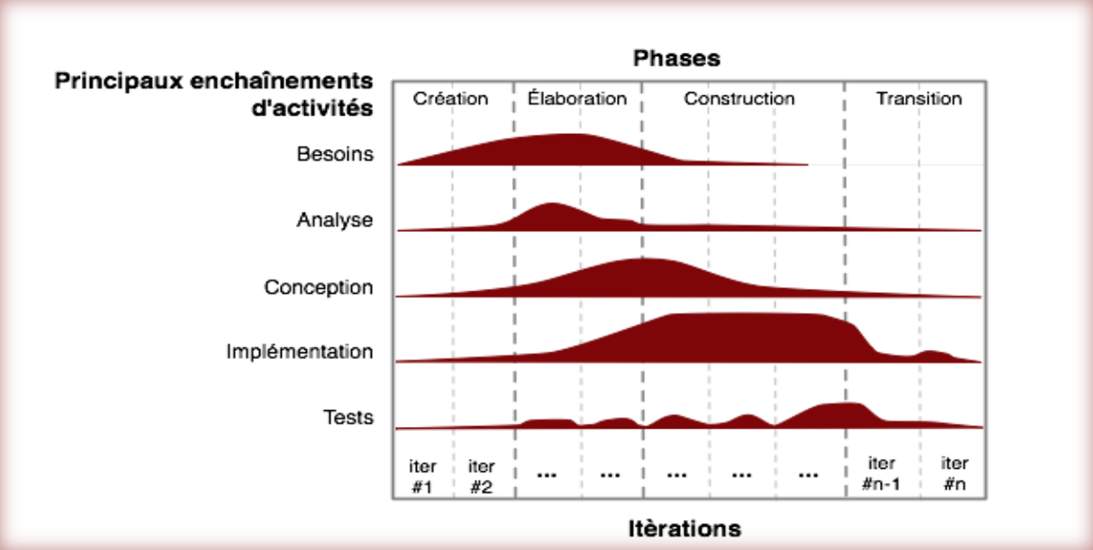
\includegraphics[width=0.8\textwidth]{processus-unifie.png}
    \caption{Cycle de vie du Processus Unifié}
    \label{fig:processus-unifie}
\end{figure}

\subsection{Langage de modélisation unifié (UML)}

UML est le langage de modélisation de la technologie objet, standard adopté par les grands acteurs du marché
Il permet de concevoir des modèles orientés objet tout en
restant indépendant de tout langage de programmation. Grâce à ses nombreux diagrammes,
UML permet de visualiser le fonctionnement des différents composants d'un système et
de détailler les spécifications techniques, facilitant ainsi la résolution des problèmes
d'intégration entre les différents modules du système \cite{guibert_uml}.

Dans ce projet, les diagrammes UML suivants sont utilisés :

\begin{itemize}[leftmargin=*, noitemsep]
    \item \textbf{Diagramme de cas d'utilisation :}
    Décrit les fonctionnalités du système du point de vue de l'utilisateur (acteur). Il
    représente les relations entre un acteur et ses besoins fonctionnels offerts
    par le système visant à produire un résultat observable et utile pour cet acteur \cite{audibert_usecase}.

    \item \textbf{Diagramme de classes :}
    Représente la structure statique du système en décrivant les différentes classes, leurs attributs, leurs opérations ainsi que les relations qui les relient, telles que l’association, la généralisation spécialisation,
     l’agrégation et la composition.
     Il constitue ainsi une vue logique de l’architecture du système
 \cite{audibert_classes}.

    \item \textbf{Diagramme de séquence :}
    Représente la séquence de messages entre les objets au cours d'une interaction.
    Il comprend un groupe d'objets, représentés par des lignes de vie, et les messages que ces objets échangent lors de l’interaction
 \cite{ibm_sequence}.

    \item \textbf{Diagramme de déploiement :}
    Présente les nœuds matériels sur lesquels le système sera réparti.
    Les nœuds peuvent êtres des ordinateurs, des détecteurs et des imprimantes, ainsi que d'autres périphériques qui prennent en charge l'environnement d'exécution d'un système
 \cite{ibm_deploiement}.

    \item \textbf{Diagramme de composants :}
   Il décrit le système modélisé sous forme de composants logiciels et met en évidence les relations de dépendance entre ces composants
   permettant ainsi de représenter l’architecture logicielle du système
 \cite{wiki_composants}.
\end{itemize}

\subsection{La méthode GIMSI}

GIMSI est une méthode coopérative de conception de systèmes d'aide à la décision,
et plus précisément d'assistance au pilotage par tableaux de bord. Structurée en
10 étapes successives, notre projet n'en nécessite que 8. Elle s'inscrit dans un
mode de management moderne, fondé sur de solides principes de gouvernance et de
développement durable. La méthode privilégie la coopération et le partage des
connaissances \cite{gimsi}.

\begin{table}[H]
\centering
\begin{tabularx}{\textwidth}{|>{\raggedright\arraybackslash}p{3cm}|>{\raggedright\arraybackslash}X|}
\hline
\textbf{Phase} & \textbf{Étapes et description} \\
\hline

\textbf{1 -- Identification} &
\textbf{Étape 1 : Environnement de l'entreprise} : Analyse de l'environnement
économique et de la stratégie de l'entreprise. \newline
\textbf{Étape 2 : Identification de l'entreprise} : Analyse des structures de
l'entreprise pour identifier les processus, activités et acteurs concernés. \\
\hline

\textbf{2 -- Conception} &
\textbf{Étape 3 : Définition des objectifs} : Sélection des objectifs tactiques en fonction de la stratégie générale. \newline
\textbf{Étape 4 : Construction du tableau de bord} : Définition du tableau de
bord de chaque équipe. \newline
\textbf{Étape 5 : Choix des indicateurs} : Choix des indicateurs en fonction
des objectifs choisis, du contexte et des acteurs concernés. \newline
\textbf{Étape 6 : Collecte des informations} : Identification des informations
nécessaires à la construction des indicateurs. \newline
\textbf{Étape 7 : Le système de tableau de bord} : Construction du système de
tableau de bord et contrôle de la cohérence globale. \\
\hline

\textbf{3 -- Mise en œuvre} &
\textbf{Étape 8 : Intégration et déploiement} : Implantation des progiciels
et déploiement au sein de l'entreprise. \\
\hline

\end{tabularx}
\caption{Les phases et les étapes de la méthode GIMSI}
\end{table}

%------------------------------------------
\section{Planification du projet : diagramme de Gantt}
%------------------------------------------

Notre projet est structuré en plusieurs activités principales bien définies, planifiées
selon des dates de début et de fin, afin de suivre l'avancement du projet de manière
visuelle.

\begin{figure}[H]
    \centering
    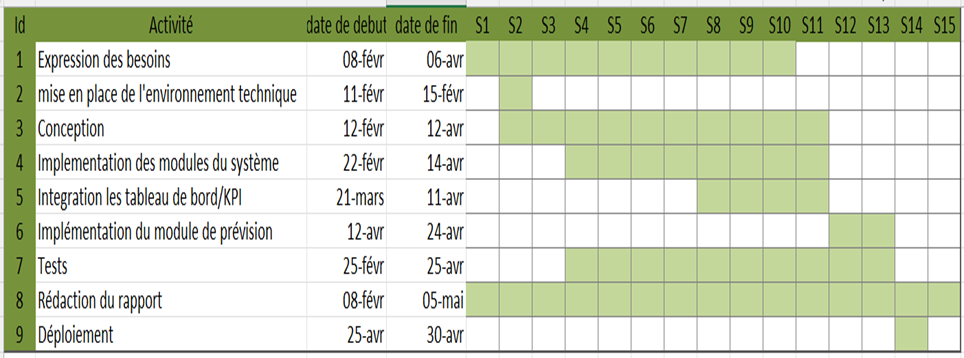
\includegraphics[width=\textwidth]{gantt.png}
    \caption{Diagramme de Gantt}
    \label{fig:gantt}
\end{figure}

%------------------------------------------
\section{Conclusion}
%------------------------------------------

Ce chapitre a présenté le contexte général du projet ainsi que l'analyse de l'existant,
mettant en évidence les limites du système actuel et la nécessité d'une solution
performante. Les objectifs du projet ont été définis, visant le développement d'une
application web de gestion des ventes intégrant des fonctionnalités de Business
Intelligence et un module de prévision. Le choix du Processus Unifié, de la
modélisation UML et de la méthode GIMSI a permis d'adopter une démarche structurée
et cohérente. Le chapitre suivant sera consacré à l'identification et à la
spécification détaillée des besoins.
\mychapter{Expression des besoins}

\section{Introduction}
Dans ce chapitre se concentre sur l'expression et l'analyse des besoins de notre système.
Dans un premier temps, nous identifions les divers acteurs qui interagissent avec le systéme
puis les besoins fonctionnels, non fonctionnels et les besoins décisionnels qui sont répertoriés dans notre système.
Enfin, nous élaborons ces besoins par des  spécifications détaillées des cas d'utilisation, présentée par un diagramme  de cas d'utilisation raffiné
\section{Identifications des acteurs}

Un acteur est une abstraction d'un rôle joué par les utilisateurs du système pouvant être une personne ou un autre système qui interagissent directement avec le système à modéliser.

Notre système est utilisé par deux acteurs :CEO (l'administrateur) et l'agent commercial.

\subsection*{CEO(Admin)}

C'est le propriétaire du dépôt de boissons, il détient le niveau d'accès le plus élevé du système.

Il bénéficie d'un accès global lui permettant de gérer l'ensemble des opérations.

Il est responsable de la gestion des comptes utilisateurs.

Il assure également le suivi des données stratégiques de l'entreprise (produits « boissons », clients, ventes, facturation et paiements) afin de prendre des décisions pertinentes et éclairées.

\subsection*{Agent commercial}

L'agent commercial est responsable de la gestion opérationnelle des activités de vente au quotidien.

Il assure le bon déroulement du processus de vente, la bonne gestion des clients et des boissons, générer des factures ainsi que la validation des paiements.

Il s'occupe également de la consultation et de l'impression des factures et de l'envoi via whatsapp

\section{Identification des besoins}

\subsection{Identification des besoins fonctionnels}
\begin{itemize}


\item \textbf{Se connecter :} Permet à l'agent commercial et CEO d'accéder au système en saisissant ses identifiants (email et mot de passe) afin d'accéder aux fonctionnalités autorisées.

\item \textbf{Gérer Produit :} Permet à l'agent commercial et au CEO d'ajouter, modifier, consulter, archiver et supprimer uniquement les boissons qui ne sont pas encore associées à une vente

\item \textbf{Gérer client:} Permet à l'agent commercial et au CEO d'ajouter, modifier, archiver, consulter les informations relatives aux clients et les supprimer uniquement s'ils ne sont pas encore associés à une vente.

\item \textbf{Traiter vente :} Permet à l'agent commercial et au CEO d'enregistrer les nouvelles ventes, de suivre leur état, de consulter l'historique des ventes et d'effectuer l'archivage d'une vente.

\item \textbf{Gérer Facture :} permet à l'agent commercial et au CEO de créer, consulter, archiver, enregistrer un règlement ainsi que de suivre les détails de paiement (mode, type, montant payé, date de paiement et date d'échéance) avec la possibilité de l'imprimer ou de l'envoyer via WhatsApp.

\item \textbf{Gérer Agent commercial :} Permet au CEO d'ajouter et de supprimer les agents commerciaux qui utilisent le système 

\item \textbf{Gérer Notification :} Permet au CEO et à l'agent commercial d'être informés en temps réel des événements critiques du système (tels que la rupture de stock d'un produit, la date d'échéance d'un règlement arrivant aujourd'hui etc.) 

Ils ont la possibilité de les marquer comme lues ou de les supprimer s'ils n'en ont plus besoin.

\item \textbf{Consulter les tableaux de bord :} Permet au CEO de visualiser les indicateurs clés de performance (KPI) et les statistiques des ventes sous forme de graphiques.

\item \textbf{Consulter les prévisions des ventes :} Permet au CEO de visualiser les prévisions des ventes futures, basées sur les données historiques des ventes, afin d'aider à la prise de décision stratégique.

\end{itemize}
\newpage


\begin{figure}[H]
  \centering
  \makebox[\textwidth][c]{%
    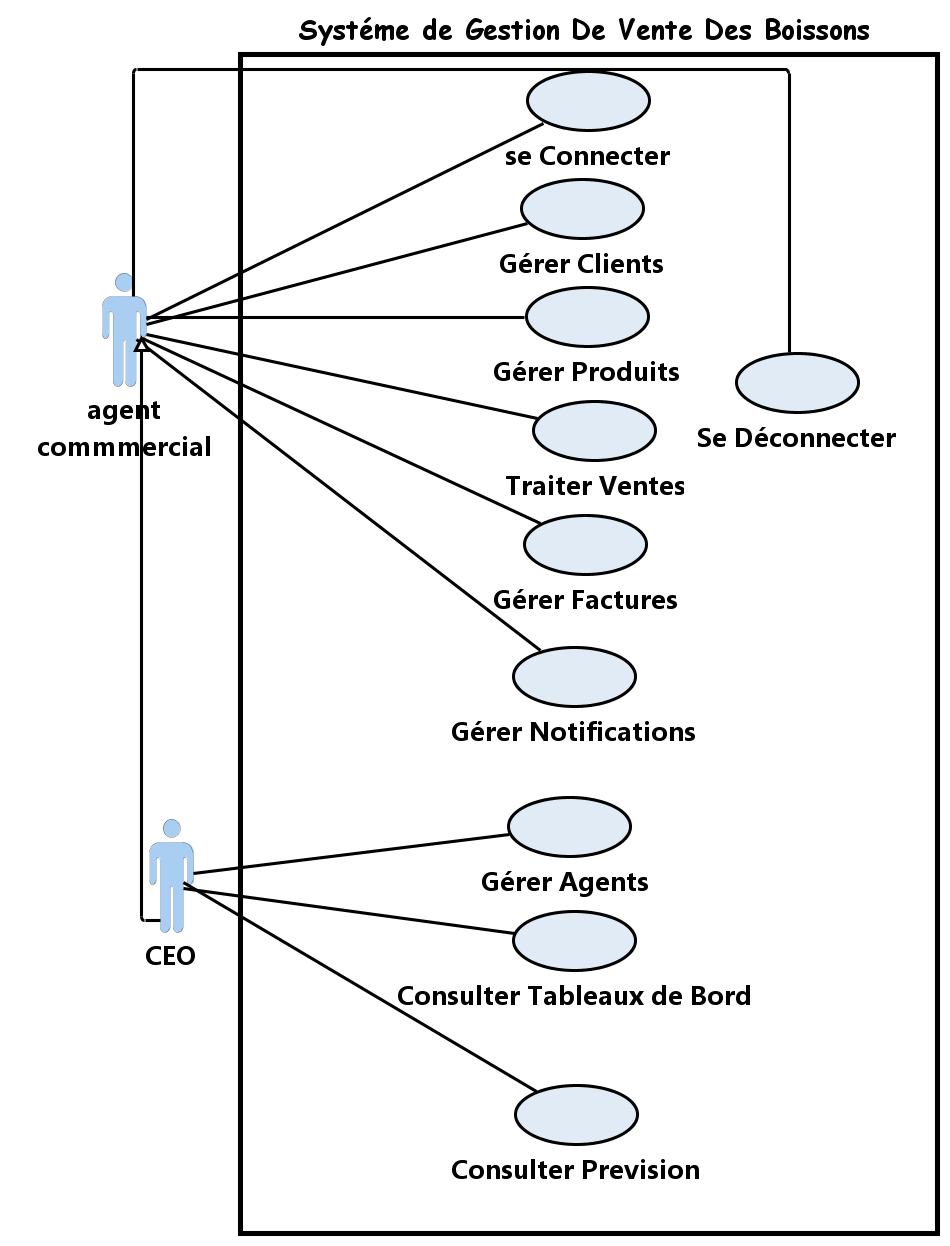
\includegraphics[width=1.2\textwidth, height=0.93\textheight]{images/MCU_DiagrammeCasUtilisationGlobal.png}%
  }
  \caption{Diagramme de cas d'utilisation globale}
  \label{fig:usecaseglobal}
\end{figure}

\newpage


\section{Identification des besoins non fonctionnels}

\begin{itemize}

\item \textbf{Sécurité :} le système protège les données des utilisateurs ainsi que les informations privilégiées (telles que les informations liées aux clients, aux ventes et aux factures).

\item \textbf{Fiabilité :} le système est capable de fonctionner d'une manière efficace, sans erreur.

\item \textbf{Ergonomie :} notre système est clair, avec une interface simple, compréhensible et intuitive. Il est également facile à utiliser.

\item \textbf{Maintenabilité :} le système est capable d'être modifié ou amélioré même après son implémentation, sans perturber l'exécution des fonctionnalités existantes.

\end{itemize}



\section{Identification des besoins décisionnels}

\subsection*{Les besoins décisionnels du CEO (Admin)}

\begin{itemize}

\item \textbf{Le suivi global des opérations du système}

Le système permet d'assurer le suivi global des opérations en mettant à disposition des données complètes et détaillées, notamment les informations relatives aux ventes, aux produits, aux factures, aux clients, aux paiements ainsi qu'aux utilisateurs du système. Cette vision globale permet au CEO de suivre et de contrôler l'ensemble des opérations afin d'assurer une gestion efficace du système.

\item \textbf{Gestion des risques}

Le système permet au CEO de détecter les anomalies liées aux transactions et au stock, notamment les ventes non réglées, les paiements au comptant ou partiels, ainsi que les anomalies concernant les produits finis en stock, afin d'assurer une prise de décision efficace et de garantir la fiabilité des opérations de ventes.

\item \textbf{Les décisions stratégiques}

Le système met à disposition du CEO des tableaux de bord stratégiques offrant une vision claire et synthétique de la situation de l'entreprise. Ces outils permettent d'identifier les produits les plus performants, les clients les plus actifs et les clients fidèles, de suivre le volume des ventes par période, le chiffre d'affaires ainsi que la répartition des paiements (au comptant ou à crédit).

Le système offre également des tableaux de prévision des ventes, permettant d'anticiper l'évolution future de l'activité à partir des données historiques.

\end{itemize}
\newpage

\section{Affectation des priorités aux cas d'utilisation}

Afin de faciliter la planification et le développement du système, nous avons attribué un niveau de priorité à chaque cas d'utilisation selon son importance dans le fonctionnement global de l'application.

Les fonctionnalités essentielles au démarrage et au bon déroulement des opérations quotidiennes ont été classées avec une priorité élevée, tandis que les fonctionnalités d'analyse, de prévision et de confort d'utilisation ont été placées à des niveaux de priorité inférieurs.

Le tableau suivant présente l'ensemble des cas d'utilisation ainsi que leur niveau de priorité.

\begin{table}[H]
\centering

\renewcommand{\arraystretch}{1.2}



\begin{tabular}{|p{9cm}|c|}
\hline
\rowcolor{purple!25}
\textbf{Cas d'utilisation} & \textbf{Priorité} \\
\hline
Se connecter & 1 \\
\hline
Gérer Produit & 1 \\
\hline
Gérer Clients & 1 \\
\hline
Gérer Agents & 1 \\
\hline
Traiter Ventes & 2 \\
\hline
Gérer Factures & 2 \\
\hline
Consulter les Tableaux de Bord & 3 \\
\hline
Consulter Prévisions & 4 \\
\hline
Gérer Notifications & 5 \\
\hline
Se Déconnecter & 5 \\
\hline
\end{tabular}

\caption{Priorité des cas d'utilisation}

\end{table}

\newpage
\section{Spécification et raffinement des cas d'utilisation}

\subsection{Spécification du cas d'utilisation Se Connecter}

\begin{table}[H]
\begin{tabularx}{\textwidth}{|l|X|}
\hline
\textbf{Titre CU :} & Se Connecter \\
\hline
\textbf{Acteur(s) :} & Agent commercial, CEO \\
\hline
\textbf{Description brève :} & Ce cas d'utilisation permet aux acteurs de se connecter afin d'accéder à leurs espaces de travail \\
\hline
\textbf{Postcondition(s)} & L'utilisateur est connecté avec succès \\
\hline
\textbf{Scénario de base :} &
\begin{enumerate}[leftmargin=1.5em, topsep=2pt, itemsep=1pt]
  \item L'utilisateur accède à la page de connexion
  \item Le système permet à l'utilisateur d'entrer son email et mot de passe
  \item L'utilisateur confirme son identification
  \item Le système vérifie la validité des information remplies
  \item Le système confirme que l'utilisateur existe et que le mot de passe correcte
  \item Le système ouvre l'espace de travail correspondant à chaque utilisateur
\end{enumerate} \\
\hline
\textbf{Autre(s) scénario(s)} &
\textbf{4.a. information obligatoires manquantes ou invalide}
\begin{enumerate}[leftmargin=1.5em, topsep=2pt, itemsep=1pt]
  \item Le système informe l'agent qu'il y a des informations obligatoires manquants
  \item Le système retourne à l'étape 2 du scénario de base
\end{enumerate}
\textbf{4.b. e-mail ou un mot de passe non reconnu}
\begin{enumerate}[leftmargin=1.5em, topsep=2pt, itemsep=1pt]
  \item Le système informe l'utilisateur que son email ou son mot de passe sont incorrecte
  \item Le système retourne à l'étape 2 de scénario de base
\end{enumerate} \\
\hline
\end{tabularx}
\caption{Spécification du CU : Se Connecter}
\label{tab:cu-connecter}
\end{table}

\newpage
\subsection{Spécification du cas d'utilisation Se Déconnecter}

\begin{table}[H]
\begin{tabularx}{\textwidth}{|l|X|}
\hline
\textbf{Titre CU :} & se Déconnecter \\
\hline
\textbf{Acteur(s) :} & Agent commercial, CEO \\
\hline
\textbf{Description brève :} & Ce cas d'utilisation permet aux acteurs de se déconnecter de leur espace de travail \\
\hline
\textbf{Pré-condition(s)} & L'utilisateur est connecté \\
\hline
\textbf{Post-condition(s)} & L'utilisateur est déconnecté du système et redirigé vers la page de connexion \\
\hline
\textbf{Scénario de base :} &
\begin{enumerate}[leftmargin=1.5em, topsep=2pt, itemsep=1pt]
  \item L'utilisateur demande de se déconnecter
  \item Le système affiche la fenêtre de déconnexion
  \item Le système demande l'utilisateur de confirmer l'opération de déconnexion
  \item L'utilisateur confirme la déconnexion
  \item Le système redirige l'utilisateur vers la page de connexion
\end{enumerate} \\
\hline
\textbf{Autre(s) scénario(s)} &
\textbf{4a. L'utilisateur demande d'annuler la déconnexion}
\begin{enumerate}[leftmargin=1.5em, topsep=2pt, itemsep=1pt]
  \item Le système informe l'utilisateur que l'opération est annulée
  \item Le système reste dans l'espace de travail
  \item Le CU Se termine
\end{enumerate} \\
\hline
\end{tabularx}
\caption{Spécification du CU : Se Déconnecter}
\label{tab:cu-deconnecter}
\end{table}

\newpage
\section{Spécification de cas d'utilisation Gérer Agents}

\subsection{Spécification du cas d'utilisation Ajouter Agents}

\begin{table}[H]
\begin{tabularx}{\textwidth}{|l|X|}
\hline
\textbf{Titre CU :} & Ajouter Agents \\
\hline
\textbf{Acteur(s) :} & CEO \\
\hline
\textbf{Description brève :} & Ce cas d'utilisation permet au CEO d'ajouter un nouvel agent dans le système en renseignant son adresse email et son mot de passe. \\
\hline
\textbf{Pré-condition(s)} & Le CEO est connecté \\
\hline
\textbf{Post-condition(s)} & Le nouvel agent est enregistré \\
\hline
\textbf{Scénario de base :} &
\begin{enumerate}[leftmargin=1.5em, topsep=2pt, itemsep=1pt]
  \item Le CEO demande la gestion des agents
  \item Le CEO demande l'ajout d'un nouvel agent
  \item Le système affiche le formulaire d'ajout
  \item Le CEO fournit les informations liées à l'agent
  \item Le CEO demande d'enregistrer les détails de l'agent
  \item Le système vérifie si toutes les informations obligatoires sont remplies et sont valides
  \item Le système vérifie si l'email existe déjà
  \item Le système enregistre le nouvel agent
  \item Le système informe le CEO que l'agent est ajouté avec succès
  \item Le système affiche l'agent dans la liste
\end{enumerate} \\
\hline
\textbf{Autre(s) scénario(s)} &
\textbf{6.a informations obligatoires manquantes}
\begin{enumerate}[leftmargin=1.5em, topsep=2pt, itemsep=1pt]
  \item Le système détecte qu'il Ya des détails obligatoires manquantes
  \item Le système informe l'agent de remplir les informations manquantes
  \item Le système retourne à l'étape 4 du scénario de base
\end{enumerate}
\textbf{7.a Email déjà enregistré dans le système}
\begin{enumerate}[leftmargin=1.5em, topsep=2pt, itemsep=1pt]
  \item Le système informe le CEO que cet email existe déjà.
  \item Le CU se Termine.
\end{enumerate} \\
\hline
\end{tabularx}
\caption{Spécification du CU : Ajouter Agent}
\label{tab:cu-ajouter-agent}
\end{table}

\newpage
\subsection{Spécification du cas d'utilisation supprimer Agent}

\begin{table}[H]
\begin{tabularx}{\textwidth}{|l|X|}
\hline
\textbf{Titre CU :} & supprimer utilisateur \\
\hline
\textbf{Acteur(s) :} & CEO \\
\hline
\textbf{Description brève :} & Ce cas d'utilisation permet au CEO de supprimer un agent existant \\
\hline
\textbf{Pré-condition(s)} & Le CEO est connecté et au moins un agent existe dans le système \\
\hline
\textbf{Post-condition(s)} & L'agent est supprimé définitivement du système et ne peut plus se connecter \\
\hline
\textbf{Scénario de base :} &
\begin{enumerate}[leftmargin=1.5em, topsep=2pt, itemsep=1pt]
  \item Le CEO demande la page Agents
  \item le systéme cherche tous les agents existants
  \item Système affiche la liste des agents.
  \item Le CEO sélectionne l'agent à supprimer.
  \item Le CEO demande de supprimer l'agent sélectionner
  \item Le système demande une confirmation de suppression.
  \item Le CEO confirme la suppression.
  \item Le système supprime définitivement l'agent
  \item Le système informe le CEO que l'agent est supprimé avec succès.
\end{enumerate} \\
\hline
\textbf{Autre(s) scénario(s)} &
\textbf{6.a. suppression annuler}
\begin{enumerate}[leftmargin=1.5em, topsep=2pt, itemsep=1pt]
  \item Le CEO demande d'annuler la suppression de l'agent
  \item Le système informe le CEO que la suppression a été annuler
  \item Le CU se termine
\end{enumerate} \\
\hline
\end{tabularx}
\caption{Spécification du CU : Supprimer Agent}
\label{tab:cu-supprimer-agent}
\end{table}

\clearpage

\section{Spécification de cas d'utilisation Gérer produit}

\subsection{Spécification de cas d'utilisation Ajouter Produit}

\begingroup
\small
\renewcommand{\arraystretch}{0.92}
\begin{longtable}{|p{3.4cm}|p{11.2cm}|}
\hline
\textbf{Titre CU :} & Ajouter Produit \\
\hline
\textbf{Acteur(s) :} & Agent commercial \\
\hline
\textbf{Description brève :} & Ce cas d'utilisation permet à l'Agent commercial d'ajouter un nouveau produit (boisson gazeuse, jus, eau) en renseignant ses informations telles que le nom du produit, la catégorie, le prix unitaire, le prix d'achat et la quantité en stock. \\
\hline
\textbf{Pré-condition(s)} & L'Agent commercial est connecté \\
\hline
\textbf{Postcondition(s)} & Le produit est enregistré avec le statut disponible à la vente ou faible \\
\hline
\textbf{Scénario de base :} &
\begin{enumerate}[leftmargin=1.5em, topsep=2pt, itemsep=1pt]
  \item L'Agent commercial demande la gestion des produits
  \item L'Agent commercial demande Ajouter produit
  \item Le système permet à l'agent commercial d'entrer les détails d'un nouveau produit
  \item L'Agent commercial fournit les informations requises
  \item L'Agent commercial demande d'enregistrer tous les détails du produit
  \item Le système vérifie si toutes les informations obligatoires sont remplies et sont valides
  \item Le système vérifie si le produit existe déjà
  \item Le système affecte un état au produit en fonction de la valeur de stock introduite par l’agent
  \item Le système enregistre le produit à l'état disponible
  \item Le système informe l'agent que le produit est ajouté avec succès
\end{enumerate} \\
\hline
\textbf{Autre(s) scénario(s)} &
\textbf{6.a informations obligatoires non remplis et non valide :}
\begin{enumerate}[leftmargin=1.5em, topsep=2pt, itemsep=1pt]
  \item Le système informe l'agent de remplir les informations manquantes
  \item Le système retourne à l'étape 4 du scénario de base
\end{enumerate}
\textbf{6.b quantite de stock = 0 :}
\begin{enumerate}[leftmargin=1.5em, topsep=2pt, itemsep=1pt]
  \item Le système informe l'agent que le stock doit être supérieur à 0
  \item Le système retourne à l'étape 4 du scénario de base
\end{enumerate}
\textbf{7.a Produit déjà enregistrer dans le système :}
\begin{enumerate}[leftmargin=1.5em, topsep=2pt, itemsep=1pt]
  \item Le système informe l'agent que le produit existe déjà
  \item Le CU se termine sans ajout d'un nouveau produit
\end{enumerate}
\textbf{9.a quantite de stock <= 5 :}
\begin{enumerate}[leftmargin=1.5em, topsep=2pt, itemsep=1pt]
  \item Le système enregistre le produit à l'état faible
\end{enumerate} \\
\hline
\caption{Spécification du CU : Ajouter Produit}
\label{tab:cu-ajouter-produit}
\end{longtable}
\endgroup

\newpage
\subsection{Spécification de cas d'utilisation supprimer produit}

\begin{table}[H]
\begin{tabularx}{\textwidth}{|l|X|}
\hline
\textbf{Titre CU :} & Supprimer produit \\
\hline
\textbf{Acteur(s) :} & Agent commercial \\
\hline
\textbf{Description brève :} & Ce cas d'utilisation permet à l'Agent commercial de supprimer un produit du système (boisson gazeuse / eau/jus). Le système vérifie si le produit est associé à des ventes déjà enregistrées, dans ce cas la suppression est refusée sinon le produit est définitivement supprimé du système \\
\hline
\textbf{Pré-condition(s)} & L'agent commercial est connecté et au moins un produit existe dans le système \\
\hline
\textbf{Post-condition(s)} & Le produit est supprimé \\
\hline
\textbf{Scénario de base :} &
\begin{enumerate}[leftmargin=1.5em, topsep=2pt, itemsep=1pt]
  \item L'Agent commercial demande la gestion des produits.
  \item <<include>> consulter produit
  \item L'Agent commercial demande de supprimer un produit
  \item Le système vérifie si le produit est associé à une vente existante
  \item Le système affiche un message pour confirmer la suppression
  \item L'Agent commercial confirme la suppression de produit
  \item Le système supprime le produit sélectionné
  \item Le système informe l'agent que le produit a été supprimé avec succès
\end{enumerate} \\
\hline
\textbf{Autre(s) scénario(s)} &
\textbf{4.a produit est associé à une vente}
\begin{enumerate}[leftmargin=1.5em, topsep=2pt, itemsep=1pt]
  \item Le système détecte que ce produit est associé à une vente
  \item Le système informe l'agent que cette suppression est impossible
  \item $\langle\langle$Extend$\rangle\rangle$ archiver Produit
  \item Le CU se termine
\end{enumerate}
\textbf{6.a Annulation de confirmation de suppression}
\begin{enumerate}[leftmargin=1.5em, topsep=2pt, itemsep=1pt]
  \item L'Agent commercial annule la suppression
  \item Le système affiche un message indiquant que l'opération de suppression a été annulé
  \item Le CU se termine
\end{enumerate} \\
\hline
\end{tabularx}
\caption{Spécification du CU : Supprimer Produit}
\label{tab:cu-supprimer-produit}
\end{table}

\newpage
\subsection{Spécification de cas d'utilisation Consulter produit}

\begin{table}[H]
\begin{tabularx}{\textwidth}{|l|X|}
\hline
\textbf{Titre CU :} & Consulter produit \\
\hline
\textbf{Acteur(s) :} & Agent commercial \\
\hline
\textbf{Description brève :} & Ce cas d'utilisation permet à l'Agent commercial d'effectuer une recherche ou un filtrage sur les produits (eau et boissons gazeuses, jus) enregistrés dans le système \\
\hline
\textbf{Pré-condition(s)} & L'agent commercial est connecté et au moins un produit existe dans le système \\
\hline
\textbf{Post-condition(s)} & Les détails du produit sont affichés à l'écran. \\
\hline
\textbf{Scénario de base :} &
\begin{enumerate}[leftmargin=1.5em, topsep=2pt, itemsep=1pt]
  \item L'Agent commercial demande la gestion des produits
  \item Le système recherche les produits enregistrés
  \item Le système affiche la liste des produits enregistres
  \item L'agent commerciale peut s'il désire, filtrer les produits par état (disponible, stock faible, repture et archivé)
  \item Si le filtre est choisi le system affiche le produits correspondants au filtre
  \item L'agent commerciale peut s'il désire, chercher le produit dans la barre de recherche
  \item Le systéme affiche les produits correspondants
  \item L'agent commerciale peut également consulter les détails d'un produit souhaité
  \item Le système affiche les détails du produit tels que : le nom, le prix unitaire, le stock et le statut.
\end{enumerate} \\
\hline
\textbf{Autre(s) scénario(s)} &
\textbf{5.a. Liste filtrage Vide}
\begin{enumerate}[leftmargin=1.5em, topsep=2pt, itemsep=1pt]
  \item Le système informe l'agent commercial qu'aucun produit ne correspond aux critères de filtrage appliqués
\end{enumerate}
\textbf{7.a. le produit recherché n'existe pas}
\begin{enumerate}[leftmargin=1.5em, topsep=2pt, itemsep=1pt]
  \item Le système affiche un message indiquant que le produit recherché n'existe pas dans le système
  \item le CU se termine
\end{enumerate} \\
\hline
\end{tabularx}
\caption{Spécification du CU : Consulter Produit}
\label{tab:cu-consulter-produit}
\end{table}

\newpage
\subsection{Spécification de cas d’utilisation modifier produit}

\begin{table}[H]
\footnotesize
\renewcommand{\arraystretch}{0.88}
\begin{tabularx}{\textwidth}{|p{3.4cm}|X|}
\hline
\textbf{Titre CU :} & Modifier produit \\
\hline
\textbf{Acteur(s) :} & Agent commercial \\
\hline
\textbf{Description brève :} & Ce cas d’utilisation permet à l’Agent commercial de modifier les informations d’un produit existant dans le système (nom, catégorie, stock, prix unitaire, statut). \\
\hline
\textbf{Pré-condition(s)} & L’agent commercial est connecté et au moins un produit enregistré dans le système \\
\hline
\textbf{Post-condition(s)} & Les modifications effectuées au produit sont enregistrées. \\
\hline
\textbf{Scénario de base :} &
\begin{enumerate}[leftmargin=1.5em, topsep=1pt, itemsep=0pt]
  \item L’Agent commercial demande la gestion des Produits
  \item <<Include>> consulter produit
  \item L’Agent commercial demande de modifier un produit
  \item Le système affiche les informations actuelles du produit
  \item L’Agent commercial modifie les informations souhaitées (nom, catégorie, prix unitaire, stock)
  \item L’Agent commercial enregistre les modifications
  \item Le système vérifie si toutes les informations obligatoires sont remplies
  \item Le système vérifie que le nom n’est pas déjà utilisé
  \item Le système affecte un état au produit en fonction de la valeur de stock introduite par l’agent
  \item Le système enregistre la modification du produit à l’état disponible
  \item Le système informe l’agent que le produit a été modifié avec succès
\end{enumerate} \\
\hline
\textbf{Autre(s) scénario(s)} &
\textbf{7.a Informations obligatoires manquantes :}
\begin{enumerate}[leftmargin=1.5em, topsep=1pt, itemsep=0pt]
  \item Le système détecte qu’il y a des détails obligatoires manquants
  \item Le système informe l’agent de remplir les informations manquantes
  \item Le système retourne à l’étape 5 du scénario de base
\end{enumerate}
\textbf{7.b Quantité de stock = 0 :}
\begin{enumerate}[leftmargin=1.5em, topsep=1pt, itemsep=0pt]
  \item Le système informe l’agent que le stock doit être supérieur à 0
  \item Le système retourne à l’étape 5 du scénario de base
\end{enumerate}
\textbf{8.a Nom déjà utilisé :}
\begin{enumerate}[leftmargin=1.5em, topsep=1pt, itemsep=0pt]
  \item Le système détecte que le nom saisi est déjà utilisé
  \item Le système informe l’agent que le produit existe déjà
  \item Le système retourne à l’étape 5 du scénario de base
\end{enumerate}
\textbf{10.a Quantité de stock $\leq$ 5 :}
\begin{enumerate}[leftmargin=1.5em, topsep=1pt, itemsep=0pt]
  \item Le système enregistre le produit à l’état faible
\end{enumerate} \\
\hline
\end{tabularx}
\caption{Spécification du CU : Modifier Produit}
\label{tab:cu-modifier-produit}
\end{table}

\newpage
\subsection{Spécification de cas d'utilisation Archiver Produit}

\begin{table}[H]
\begin{tabularx}{\textwidth}{|l|X|}
\hline
\textbf{Titre :} & Archiver Produit \\
\hline
\textbf{Acteur :} & Agent commercial \\
\hline
\textbf{Description brève :} & Ce cas d'utilisation permet à l'Agent commercial d'archiver un produit existant dans le système. L'archivage désactive le produit sans le supprimer définitivement, afin qu'il ne soit plus disponible à la vente ni visible dans la liste active des produits. \\
\hline
\textbf{Précondition :} & L'Agent commercial est connecté et au moins un Produit est enregistré dans le système \\
\hline
\textbf{Post condition :} & Le produit est archivé et n'apparaît plus dans la liste active des produits. \\
\hline
\textbf{Scenario de base :} &
\begin{enumerate}[leftmargin=1.5em, topsep=2pt, itemsep=1pt]
  \item L'agent commerciale demande la gestion des produits
  \item <<include>>Consulter produit
  \item L'agent commercial demande d'archiver un produit
  \item Le système demande la confirmation de l'opération d'archivage.
  \item L'agent commercial confirme l'archivage
  \item Le système affecte un état au produit archivé
  \item Le système archive le produit.
  \item Le système informe l'agent que le produit a été archivé avec succès.
\end{enumerate} \\
\hline
\textbf{Autre(s) scénario(s) :} &
\textbf{5.a. L'agent annule l'archivage :}
\begin{enumerate}[leftmargin=1.5em, topsep=2pt, itemsep=1pt]
  \item L'agent commercial demande d'annuler l'opération
  \item Le système annule l'archivage
  \item Le CU se termine
\end{enumerate} \\
\hline
\end{tabularx}
\caption{Spécification du CU : Archiver Produit}
\label{tab:cu-archiver-produit}
\end{table}

\newpage
\section{Spécification de cas d'utilisation Gérer clients}

\subsection{Spécification d'Ajouter Client}

\begin{longtable}{|>{\bfseries}p{3.5cm}|p{\dimexpr\textwidth-3.5cm-4\tabcolsep-2\arrayrulewidth}|}
\hline
Titre : & ajouter Client \\
\hline
Acteur : & Agent commercial \\
\hline
Description brève : & Ce cas d'utilisation permet à l'Agent commercial d'ajouter un nouveau client au système. Il choisi le type de client et introduit les informations nécessaires (prénom, nom, téléphone, e-mail, adresse et ville s'il s'agit d'une personne et il introduit nom de societe, mail, telephone, adresse, ville et matricule fisacl s'il s'agit d'une entreprise). L'ajout est possible uniquement si le client n'est pas déjà enregistré dans le système. \\
\hline
Précondition : & L'agent commercial est connecté \\
\hline
Post-condition : & Client enregistre avec succès et devient disponible pour être associé à une vente \\
\hline
Scénario de base : &
\begin{enumerate}[leftmargin=1.5em, topsep=2pt, itemsep=1pt]
  \item L'Agent commercial demande la gestion des clients
  \item L'Agent commercial demande Ajouter client
  \item Le système permet à l'agent commercial d'entrer les détails d'un nouveau client
  \item L'Agent commercial fournit les informations requises
  \item L'Agent commercial demande d'enregistre tous les details du clients
  \item Le système vérifie si toutes les informations obligatoires sont remplies et sont valides
  \item Le système vérifie si le client existe déjà
  \item Le système enregistre le client 
  \item Le système informe l'agent que le client est ajouté avec succès
\end{enumerate} \\
\hline
Autre(s) scénario(s) : &
\textbf{6.a information obligatoire non remplie :}
\begin{enumerate}[leftmargin=1.5em, topsep=2pt, itemsep=1pt]
  \item Le système détecte qu'il y a des détails obligatoires manquants
  \item Le système informe l'agent de remplir les informations manquantes
  \item Le système retourne à l'étape 4 du scénario de base
\end{enumerate}
\textbf{6.b Numéro de téléphone invalide (moins de 8 chiffres) :}
\begin{enumerate}[leftmargin=1.5em, topsep=2pt, itemsep=1pt]
  \item Le système détecte que le numéro de téléphone contient moins de 8 chiffres.
  \item Le système affiche un message indiquant que le numéro de téléphone doit contenir 8 chiffres.
  \item Le système retourne à l'étape 4 du scénario de base
\end{enumerate}
\textbf{7.a email, matricule fiscal ou numero de téléphone déjà enregistré dans le système :}
\begin{enumerate}[leftmargin=1.5em, topsep=2pt, itemsep=1pt]
  \item Le système détecte que l'email, matricule fiscal ou le numéro est déjà utilisé
  \item Le système informe l'agent que le client existe déjà
  \item Le système retourne à l'étape 4 du scénario de base
\end{enumerate} \\
\hline
\caption{Spécification du CU : Ajouter Client}
\label{tab:cu-ajouter-client}
\end{longtable}

\newpage
\subsection{Spécification de cas d'utilisation Supprimer Client}

\begin{longtable}{|>{\bfseries\raggedright\arraybackslash}p{3.5cm}|p{\dimexpr\textwidth-3.5cm-4\tabcolsep-2\arrayrulewidth}|}
\hline
Titre : & Supprimer client \\
\hline
Acteur : & Agent commercial \\
\hline
Description brève : & Ce cas d'utilisation permet à l'agent commercial de supprimer un client du système. Le système vérifie si le client est associé à des ventes déjà enregistrées ; dans ce cas, la suppression est refusée. Sinon, le client est définitivement supprimé du système et ne peut plus être utilisé dans une vente \\
\hline
Précondition : & L'agent commercial est connecté et au moins un client existe dans le système \\
\hline
Post-condition : & Le client est définitivement supprimé du système \\
\hline
Scénario de base : &
\begin{enumerate}[leftmargin=1.5em, topsep=2pt, itemsep=1pt]
  \item L'Agent commercial demande la gestion des Clients.
  \item <<Include>> consulter Clients
  \item L'Agent commercial demande de supprimer client
  \item Le système vérifie si le client est associé à des ventes existantes
  \item Le système affiche un message pour confirmer la suppression
  \item L'Agent commercial confirme la suppression de client
  \item Le système supprime le client sélectionné
  \item Le système informe l'agent que le client a été supprimé avec succès
\end{enumerate} \\
\hline
Autre(s) scénario(s) : &
\textbf{4.a Le client est associé à une vente}
\begin{enumerate}[leftmargin=1.5em, topsep=2pt, itemsep=1pt]
  \item Le système détecte que ce client est associé à une vente
  \item Le système informe l'agent que la suppression d'un client ayant effectué une vente est impossible
  \item <<Extend>> archiver Client
  \item Le CU se termine
\end{enumerate}
\textbf{6.a Annulation de confirmation de suppression}
\begin{enumerate}[leftmargin=1.5em, topsep=2pt, itemsep=1pt]
  \item L'Agent commercial annule la suppression
  \item Le système annule l'opération
  \item Le CU se termine
\end{enumerate} \\
\hline
\caption{Spécification du CU : Supprimer Client}
\label{tab:cu-supprimer-client}
\end{longtable}

\needspace{6\baselineskip}
\subsection{Spécification de cas d'utilisation Consulter Client}

\begin{longtable}{|>{\bfseries\raggedright\arraybackslash}p{3.5cm}|p{\dimexpr\textwidth-3.5cm-4\tabcolsep-2\arrayrulewidth}|}
\hline
Titre : & Consulter client \\
\hline
Acteur : & Agent commercial \\
\hline
Description brève : & Ce cas d'utilisation permet à l'Agent commercial d'effectuer une recherche ou un filtrage sur les clients afin d'accéder aux informations détaillées d'un client enregistré dans le système y compris ses ventes \\
\hline
Précondition : & L'agent commercial est connecté et au moins un client est enregistré dans le système \\
\hline
Post-condition : & Les détails du client sont affichés \\
\hline
Scénario de base : &
\begin{enumerate}[leftmargin=1.5em, topsep=2pt, itemsep=1pt]
  \item L'Agent commercial demande la gestion des Clients
  \item Le système recherche les clients enregistres dans le systéme
  \item Le système affiche la liste des clients enregistres
  \item L'agent commercial peut s'il désire, filtrer les clients par statut ou types (personne, entreprise, archivé)
  \item Si le filtre est choisi le systém affiche les client correspondants au filtre
  \item L'agent commercial peut s'il désire, chercher les clients dans la barre de recherche
  \item Le systéme affiche les clients correspondants
  \item L'agent commerciale peut egalement consulter les détails d'un client souhaité
  \item Le système affiche les détails du client tels que : nom, prenon, email, téléphone, date de création, type, ville, adresse ou nom de societe, email, téléphone, date de création, type, ville, adresse, matricule fiscal et ses ventes
\end{enumerate} \\
\hline
Autre(s) scénario(s) : &
\textbf{5.a. liste filtrage vide}
\begin{enumerate}[leftmargin=1.5em, topsep=2pt, itemsep=1pt]
  \item Le système affiche un message indiquant qu'aucun client ne correspond aux critères de filtrage appliqués
  \item Le CU se termine
\end{enumerate}
\textbf{7.a. le client recherché n'existe pas}
\begin{enumerate}[leftmargin=1.5em, topsep=2pt, itemsep=1pt]
  \item Le système affiche un message indiquant que le client recherché n'existe pas dans le système
  \item Le CU se termine
\end{enumerate} \\
\hline
\caption{Spécification du CU : Consulter Client}
\label{tab:cu-consulter-client}
\end{longtable}

\subsection{Spécification de cas d'utilisation Modifier Client}

\begin{table}[H]
\footnotesize
\renewcommand{\arraystretch}{0.88}
\begin{tabularx}{\textwidth}{|p{3.4cm}|X|}
\hline
\textbf{Titre :} & Modifier Client \\
\hline
\textbf{Acteur :} & Agent commercial \\
\hline
\textbf{Description brève :} & Ce cas d'utilisation permet à l'Agent commercial de modifier les informations d'un client qui existe dans le système (telles que : prénom, nom, téléphone, e-mail, adresse et ville pour une personne physique ou nom de société, téléphone, email, adresse, ville, matricule fiscal pour entreprise). \\
\hline
\textbf{Pré-condition :} & L'agent commercial est connecté et au moins un client est enregistré \\
\hline
\textbf{Post condition :} & Les modifications effectuées au client sont enregistrées avec succès. \\
\hline
\textbf{Scenario de base :} &
\begin{enumerate}[leftmargin=1.5em, topsep=1pt, itemsep=0pt]
  \item L'Agent commercial demande la gestion des clients.
  \item <<Include>> consulter clients.
  \item L'Agent commercial demande de modifier le client.
  \item Le système affiche les informations actuelles du client.
  \item L'Agent commercial modifie les informations souhaitées (nom, prénom, email, telephone, matricule-fiscale, ville, adresse).
  \item Le système enregistre les modifications.
  \item Le système vérifie si toutes les informations obligatoires sont remplies et valides.
  \item Le système vérifie que les nouvelles informations ne sont pas déjà utilisées.
  \item Le système enregistre la modification du client.
  \item Le système informe l'agent que le client a été modifié avec succès.
\end{enumerate} \\
\hline
\textbf{Autre(s) scenario(s) :} &
\textbf{7.a Informations obligatoires manquantes :}
\begin{enumerate}[leftmargin=1.5em, topsep=1pt, itemsep=0pt]
  \item Le système détecte qu'il y a des détails obligatoires manquants.
  \item Le système informe l'agent de remplir les informations manquantes.
  \item Le système retourne à l'étape 4 du scénario de base.
\end{enumerate}
\textbf{8.a Informations client déjà utilisées :}
\begin{enumerate}[leftmargin=1.5em, topsep=1pt, itemsep=0pt]
  \item Le système détecte que l'email ou le numéro est déjà utilisé.
  \item Le système informe l'agent que le client existe déjà.
  \item Le système retourne à l'étape 4 du scénario de base.
\end{enumerate} \\
\hline
\end{tabularx}
\caption{Spécification du CU : Modifier Client}
\label{tab:cu-modifier-client}
\end{table}
\subsection{Spécification de cas d'utilisation Archiver Client}

\begin{longtable}{|>{\bfseries\raggedright\arraybackslash}p{3.5cm}|p{\dimexpr\textwidth-3.5cm-4\tabcolsep-2\arrayrulewidth}|}
\hline
Titre : & Archiver client \\
\hline
Acteur : & Agent commercial \\
\hline
Description brève : & Ce cas d'utilisation permet à l'Agent commercial d'archiver un client enregistré dans le système, afin de le désactiver sans le supprimer définitivement du système. \\
\hline
Précondition : & L'Agent commercial est connecté et au moins un client est enregistré dans le système \\
\hline
Post-condition : & Le client est archivé et n'apparaît plus dans la liste des clients \\
\hline
Scénario de base : &
\begin{enumerate}[leftmargin=1.5em, topsep=2pt, itemsep=1pt]
  \item L'Agent commercial demande la gestion des Clients
  \item <<Include>> consulter Clients
  \item L'agent commercial demande d'archiver client
  \item Le système affiche un message pour confirmer l'archivage.
  \item L'agent commercial confirme l'archivage de client.
  \item Le système affecte un état au client archivé
  \item Le système archive le client.
  \item Le système informe l'agent que le client a été archivé avec succès
 
\end{enumerate} \\
\hline
Autre(s) scénario(s) : &
\textbf{5.a. L'agent annule l'archivage :}
\begin{enumerate}[leftmargin=1.5em, topsep=2pt, itemsep=1pt]
  \item L'agent commercial annule la confirmation.
  \item Le system annule l'opération
  \item Le CU se termine.
\end{enumerate} \\
\hline
\caption{Spécification du CU : Archiver Client}
\label{tab:cu-archiver-client}
\end{longtable}

\newpage
\needspace{6\baselineskip}
\section{Spécification de cas d'utilisation : traiter Ventes}

\subsection{Spécification de cas d'utilisation Enregistrer vente}

\begin{longtable}{|>{\bfseries\raggedright\arraybackslash}p{3.5cm}|p{\dimexpr\textwidth-3.5cm-4\tabcolsep-2\arrayrulewidth}|}
\hline
Titre : & Enregistrer vente \\
\hline
Acteur : & Agent commercial \\
\hline
Description brève : & Ce cas d'utilisation permet à l'agent commercial d'enregistrer une nouvelle vente en sélectionnant un client, un produit, une quantité et une date de vente. \\
\hline
Précondition : & L'agent commercial est connecté et au moins un client et un produit existent dans le système \\
\hline
Post-condition : & La vente est enregistrée avec succès et le stock des produits est mis à jour \\
\hline
Scénario de base : &
\begin{enumerate}[leftmargin=1.5em, topsep=2pt, itemsep=1pt]
  \item L'agent commercial demande la gestion des Ventes
  \item L'agent commercial demande Ajouter Vente
  \item Le système permet à l'agent commercial de choisir les informations nécessaires d'une nouvelle vente.
  \item L'agent commercial sélectionne un client, un ou plusieurs produit(s), fournit la quantité de chaque produit et la date de vente
  \item Le système vérifie si les quantités choisies sont disponibles dans le stock des produits concernés
  \item Le système calcule automatiquement le total de chaque  ligne de vente à partir du prix unitaire des produits et des quantités vendues
  \item le systéme desactiver la selectionne de ce produit dans cette vente
  \item L'agent commercial demande d'enregistrer l'ajoute de la nouvelle vente
  \item Le système vérifie si toutes les informations obligatoires sont remplies et sont valides
  \item Le système enregistre la vente avec un statut non payée par défaut
  \item Le système informe l'agent que la vente est enregistrée avec succès
  \item le systeme met a jour le stock des produits
  \item le systeme envoi une notification informe l'agent que le produit en repture ou faible
\end{enumerate} \\
\hline
Autre(s) scénario(s) : &
\textbf{5.a Quantité supérieure au stock disponible}
\begin{enumerate}[leftmargin=1.5em, topsep=2pt, itemsep=1pt]
  \item Le système informe l'agent que la quantité demandée dépasse le stock disponible du produit concerné
  \item Le système revient à l'étape 4 du scenario de base
\end{enumerate}
\textbf{9.a. informations de ventes obligatoires manquantes}
\begin{enumerate}[leftmargin=1.5em, topsep=2pt, itemsep=1pt]
  \item Le système détecte qu'il ya des champs obligatoires manquants
  \item Le système informe l'agent de remplir les informations manquants
  \item Le système retourne à l'étape 4 du scénario de base
\end{enumerate} \\
\hline
\caption{Spécification du CU : Enregistrer Vente}
\label{tab:cu-enregistrer-vente}
\end{longtable}

\newpage
\needspace{6\baselineskip}
\subsection{Spécification de cas d'utilisation Consulter Vente}

\begin{longtable}{|>{\bfseries\raggedright\arraybackslash}p{3.5cm}|p{\dimexpr\textwidth-3.5cm-4\tabcolsep-2\arrayrulewidth}|}
\hline
Titre : & Consulter Vente \\
\hline
Acteur : & Agent commercial \\
\hline
Description brève : & Ce cas d'utilisation permet à L'Agent commercial d'effectuer une recherche ou un filtrage sur les ventes afin d'accéder aux informations détaillées d'une vente enregistrée dans le système y compris sa facture si elle existe \\
\hline
Précondition : & L'agent commercial est connecté et au moins une vente enregistrée dans le système \\
\hline
Post-condition : & Les Details de la vente affiché à l'écran \\
\hline
Scénario de base : &
\begin{enumerate}[leftmargin=1.5em, topsep=2pt, itemsep=1pt]
  \item L'Agent commercial demande la gestion des ventes
  \item Le système recherche les ventes enregistrées dans le système
  \item Le système affiche la liste des ventes enregistrées
  \item L'agent commercial peut s'il désire, filtrer les ventes par statut (payée, non payée, partiellement payée, archivée)
  \item Si le filtre est choisi le systém affiche les ventes correspondants au filtre
  \item L'agent commercial peut s'il désire, chercher la vente dans la barre de recherche
  \item Le systéme affiche les ventes correspondants
  \item L'agent commercial peut s'il désire, consulter détails de vente souhaitées
  \item Le système affiche les détails de la vente tels que : client, produits, quantités, total, date de création, statut, sa facture et détails de facture
  \item <<Extend>>Imprimer facture
  \item <<Extend>> envoyer via WhatsApp
\end{enumerate} \\
\hline
Autre(s) scénario(s) : &
\textbf{5.a. liste filtrage vide}
\begin{enumerate}[leftmargin=1.5em, topsep=2pt, itemsep=1pt]
  \item Le système affiche un message indiquant qu'aucune vente ne correspond aux critères de filtrage appliqués
  \item Le CU se termine
\end{enumerate}
\textbf{7.a. la vente recherchée n'existe pas}
\begin{enumerate}[leftmargin=1.5em, topsep=2pt, itemsep=1pt]
  \item Le système affiche un message indiquant que la vente recherchée n'existe pas dans le système
  \item le CU se termine
\end{enumerate} \\
\hline
\caption{Spécification du CU : Consulter Vente}
\label{tab:cu-consulter-vente}
\end{longtable}

\newpage
\needspace{6\baselineskip}
\subsection{Spécification de cas d'utilisation Archiver Vente}

\begin{longtable}{|>{\bfseries\raggedright\arraybackslash}p{3.5cm}|p{\dimexpr\textwidth-3.5cm-4\tabcolsep-2\arrayrulewidth}|}
\hline
Titre : & Archiver Vente \\
\hline
Acteur : & Agent commercial \\
\hline
Description brève : & Ce cas d'utilisation permet à l'Agent commercial d'archiver une vente totalement payée dans le système, afin de la désactiver sans le supprimer définitivement du système .l'archivage d'une vente payée entraîne automatiquement l'archivage de sa facture\\
\hline
Précondition : & L'agent commercial est connecté et au moins une vente enregistrée dans le système \\
\hline
Post-condition : & La vente est archivée et n'apparaît plus dans la liste des ventes affiché \\
\hline
Scénario de base : &
\begin{enumerate}[leftmargin=1.5em, topsep=2pt, itemsep=1pt]
  \item L'agent commercial demande la gestion des ventes
  \item <<include>> Consulter ventes
  \item L'agent commercial demande d'archiver la vente
  \item Le système vérifie que la vente est totalement payée
  \item Le système informe l'agent que l'archivage de la vente entraine par defaut l'archivage automatique de la facture associée et demande la confirmation de cette opération
  \item L'agent commercial confirme l'action
  \item Le système affecte un état à la vente archivée
  \item Le systéme archive la facture associée à la vente
  \item Le système archive la vente
  \item Le système affiche un message indiquant que la vente et sa facture ont été archivées avec succès
\end{enumerate} \\
\hline
Autre(s) scénario(s) : &
\textbf{4.a. la vente est non payée ou partiellement payée.}
\begin{enumerate}[leftmargin=1.5em, topsep=2pt, itemsep=1pt]
  \item Le système informe l'agent que l'archivage d'une vente qui n'est pas encore totalement payée est impossible.
  \item Le CU se termine
\end{enumerate}
\textbf{6.a. L'agent annule l'archivage :}
\begin{enumerate}[leftmargin=1.5em, topsep=2pt, itemsep=1pt]
  \item L'agent commercial annule l'archivage.
  \item Le système annule l'opération.
  \item Le CU se termine
\end{enumerate} \\
\hline
\caption{Spécification du CU : Archiver Vente}
\label{tab:cu-archiver-vente}
\end{longtable}

\newpage
\section{Spécification de cas d'utilisation : Gérer Factures}

\subsection{Spécification de cas d'utilisation Créer Facture via facture}

\begin{longtable}{|>{\bfseries\raggedright\arraybackslash}p{3.5cm}|p{\dimexpr\textwidth-3.5cm-4\tabcolsep-2\arrayrulewidth}|}
\hline
Titre : & Créer Facture via facture \\
\hline
Acteur : & Agent commercial \\
\hline
Description brève : & Ce cas d'utilisation permet à l'agent commercial d'ajouter une facture associée à une Vente existante. \\
\hline
Pré condition : & Au moins une vente existe dans le système \\
\hline
Post-condition : & Facture ajouté dans la liste des factures \\
\hline
Scénario de base : &
\begin{enumerate}[leftmargin=1.5em, topsep=2pt, itemsep=1pt]
  \item L'agent commercial demande la gestion des factures
  \item L'agent commerciale demande Ajouter facture
  \item Le système cherche les ventes sans facture
  \item Le système permet à l'agent commercial de choisir une vente
  \item L'agent commercial choisi une vente et renseigne la date d'échéance
  \item L'Agent commercial demande d'enregistrer la facture de cette vente
  \item Le système vérifie si toutes les informations obligatoires sont remplies et sont valides
  \item Le système Créer la facture avec un statut non payée par défaut
  \item Le système informe l'agent que la facture ajoutée avec succès
\end{enumerate} \\
\hline
Autre(s) scénario(s) : &
\textbf{4.a Le système ne trouve aucune vente sans facture :}
\begin{enumerate}[leftmargin=1.5em, topsep=2pt, itemsep=1pt]
  \item Le système affiche une liste vide.
  \item Le CU se termine
\end{enumerate}
\textbf{7.a informations obligatoires manquantes :}
\begin{enumerate}[leftmargin=1.5em, topsep=2pt, itemsep=1pt]
  \item Le système détecte qu'il y a des informations obligatoires manquants
  \item Le système informe l'agent de remplir les informations manquantes
  \item Le système retourne à l'étape 4 du scénario de base
\end{enumerate}
\textbf{7.b Date d'échéance invalide :}
\begin{enumerate}[leftmargin=1.5em, topsep=2pt, itemsep=1pt]
  \item Le système informe l'agent que la date d'échéance ne doit pas être inférieure à la date de création
  \item Le système retourne à l'étape 4 du scénario de base
\end{enumerate} \\
\hline
\caption{Spécification du CU : Créer Facture via Facture}
\label{tab:cu-creer-facture-facture}
\end{longtable}

\newpage
\subsection{Spécification de cas d'utilisation Créer Facture via Vente}

\begin{longtable}{|>{\bfseries\raggedright\arraybackslash}p{3.5cm}|p{\dimexpr\textwidth-3.5cm-4\tabcolsep-2\arrayrulewidth}|}
\hline
Titre : & Créer Facture via vente \\
\hline
Acteur : & Agent commercial \\
\hline
Description brève : & Ce cas d'utilisation permet à l'agent commercial de valider la création d'une facture associée à une Vente existante. \\
\hline
Pré condition : & Au moins une vente existe dans le système \\
\hline
Post-condition : & Facture ajouté dans la liste des factures \\
\hline
Scénario de base : &
\begin{enumerate}[leftmargin=1.5em, topsep=2pt, itemsep=1pt]
  \item L'agent commercial demande la gestion des ventes
  \item <<include>>consulter Vente
  \item Le système vérifie que la vente sélectionnée n'est pas encore associée à une facture.
  \item L'agent commercial demande de créer une facture pour cette vente
  \item Le système permet à l'agent commercial de renseigne la date d'echéance
  \item L'Agent commercial demande d'enregistrer la facture de cette vente
  \item Le système vérifie si toutes les informations obligatoires sont remplies et sont valides
  \item Le système Créer la facture avec un statut non payée par défaut
  \item Le système informe l'agent que la facture ajoutée avec succès
\end{enumerate} \\
\hline
Autre(s) scénario(s) : &
\textbf{3.a Une facture a déjà été créée pour cette vente :}
\begin{enumerate}[leftmargin=1.5em, topsep=2pt, itemsep=1pt]
  \item Le système désactive l'option de creation de facture
  \item Le CU se termine
\end{enumerate}
\textbf{7.a informations obligatoires manquantes :}
\begin{enumerate}[leftmargin=1.5em, topsep=2pt, itemsep=1pt]
  \item Le système détecte qu'il ya des informations obligatoires manquants
  \item Le système informe l'agent de remplir les informations manquants
  \item Le système retourne à l'étape 4 du scénario de base
\end{enumerate}
\textbf{7.b Date d'échéance invalide :}
\begin{enumerate}[leftmargin=1.5em, topsep=2pt, itemsep=1pt]
  \item Le système informe l'agent que la date d'échéance ne doit pas être inférieure à la date de création
  \item Le système retourne à l'étape 4 du scénario de base
\end{enumerate} \\
\hline
\caption{Spécification du CU : Créer Facture via Vente}
\label{tab:cu-creer-facture-vente}
\end{longtable}

\newpage
\subsection{Spécification de cas d'utilisation Enregistrer Règlement}

\begin{longtable}{|>{\bfseries\raggedright\arraybackslash}p{3.5cm}|p{\dimexpr\textwidth-3.5cm-4\tabcolsep-2\arrayrulewidth}|}
\hline
Titre : & Enregistrer Règlement \\
\hline
Acteur : & Agent commercial \\
\hline
Description brève : & Ce cas d'utilisation permet à l'agent commercial d'enregistrer un règlement associé à une facture. Il consiste à saisir les informations du paiement (montant, date et mode de paiement). \\
\hline
Pré condition : & L'agent commercial est connecté et au moins une facture est créée dans le systéme \\
\hline
Post-condition : & Le montant restant de la facture est mis à jour, le règlement est ajouté dans l'historique, et le statut de la facture ainsi que celui de la vente associée sont mis à jour (payée ou partiellement-payée). \\
\hline
Scénario de base : &
\begin{enumerate}[leftmargin=1.5em, topsep=2pt, itemsep=1pt]
  \item L'Agent commercial demande la gestion des Factures.
  \item <<Include>> consulter Factures
  \item Le système vérifie que la facture sélectionnée n'est pas totalement payée
  \item L'agent commercial demande d'Enregistrer règlement
  \item Le système permet à l'agent commercial d'entrer les informations de ce paiement (montant a payée, date, mode de paiement)
  \item L'agent commercial fournit les informations requises
  \item L'Agent commercial confirme l'enregistrement de ce paiement
  \item Le système vérifie si toutes les informations obligatoires sont remplies et valides
  \item Le système vérifie que le montant saisi n'excède pas au reste à paye de la facture
  \item Le système enregistrer le règlement
  \item Le système met à jour le statut de facture en fonction de la valeur de nouveau reste
  \item Le système met à jour le statut de vente
  \item Le système met à jour le montant restant
  \item le systéme informe l'agent du statut de le facture
\end{enumerate} \\
\hline
Autre(s) scénario(s) : &
\textbf{3.a la facture selectionnée est déjà soldée :}
\begin{enumerate}[leftmargin=1.5em, topsep=2pt, itemsep=1pt]
  \item Le système désactive l'option d'enregistrement du réglement
  \item Le CU se termine
\end{enumerate}
\textbf{8.a champs obligatoires non remplis :}
\begin{enumerate}[leftmargin=1.5em, topsep=2pt, itemsep=1pt]
  \item Le système informe l'agent de remplir les informations manquantes
  \item Le système retourne à l'étape 5 du scénario de base
\end{enumerate}
\textbf{8.b date de règlement $<$ date de facture :}
\begin{enumerate}[leftmargin=1.5em, topsep=2pt, itemsep=1pt]
  \item Le système informe l'agent commercial que la date de règlement doit être supérieure ou égale à la date de facture.
  \item Le système retourne à l'étape 5 du scénario de base
\end{enumerate}
\textbf{9 .a montant saisi $>$ reste :}
\begin{enumerate}[leftmargin=1.5em, topsep=2pt, itemsep=1pt]
  \item Le système informe l'agent commercial que le montant ne doit pas dépasser le reste
  \item Le système retourne à l'étape 5 du scénario de base
\end{enumerate} \\
\hline
\caption{Spécification du CU : Enregistrer Règlement}
\label{tab:cu-enregistrer-reglement}
\end{longtable}

\newpage
\needspace{6\baselineskip}
\subsection{Spécification de cas d'utilisation imprimer facture}

\begin{longtable}{|>{\bfseries\raggedright\arraybackslash}p{3.5cm}|p{\dimexpr\textwidth-3.5cm-4\tabcolsep-2\arrayrulewidth}|}
\hline
Titre : & imprimer Facture \\
\hline
Acteur : & Agent commercial \\
\hline
Description brève : & Ce cas d'utilisation permet à l'agent commercial d'imprimer une facture au format papier \\
\hline
Pré condition : &
\begin{itemize}[leftmargin=1.5em, topsep=0pt, itemsep=0pt, parsep=0pt]
  \item L'agent commercial est connecté
  \item Au moins une facture existe dans le système
\end{itemize} \\
\hline
Post-condition : & Facture imprimée \\
\hline
Scénario de base : &
\begin{enumerate}[leftmargin=1.5em, topsep=2pt, itemsep=1pt]
  \item L'Agent commercial demande la gestion des Factures.
  \item <<include>> consulter Factures
  \item L'agent commercial demande d'imprimer la facture
  \item Le système génère la facture en format PDF
  \item Le système ouvre la boîte de dialogue Impression
\end{enumerate} \\
\hline
\caption{Spécification du CU : Imprimer Facture}
\label{tab:cu-imprimer-facture}
\end{longtable}

\newpage
\needspace{6\baselineskip}
\subsection{Spécification de cas d'utilisation Envoyer facture via WhatsApp}

\begin{longtable}{|>{\bfseries\raggedright\arraybackslash}p{3.5cm}|p{\dimexpr\textwidth-3.5cm-4\tabcolsep-2\arrayrulewidth}|}
\hline
Titre : & envoyer facture via WhatsApp \\
\hline
Acteur : & Agent commercial(principal)
,whatsapp(secondaire) \\
\hline
Description brève : & Ce cas d'utilisation permet à l'agent commercial d'envoyer directement au client une facture via WhatsApp \\
\hline
Pré condition : &
\begin{itemize}[leftmargin=1.5em, topsep=0pt, itemsep=0pt, parsep=0pt]
  \item L'agent commercial est connecté
  \item Au moins une facture existe dans le système
\end{itemize} \\
\hline
Post-condition : & Facture est envoyée via WhatsApp. \\
\hline
Scénario de base : &
\begin{enumerate}[leftmargin=1.5em, topsep=2pt, itemsep=1pt]
  \item L'Agent commercial demande la gestion des Factures
  \item <<include>> consulter Factures
  \item L'agent commercial demande d'Envoyer facture via WhatsApp
  \item Le système ouvre WhatsApp avec lien de facture
  \item L'agent commercial confirme l'envoi
\end{enumerate} \\
\hline
\caption{Spécification du CU : Envoyer Facture via WhatsApp}
\label{tab:cu-envoyer-whatsapp}
\end{longtable}

\subsection{Spécification de cas d'utilisation : Consulter Facture}

\begin{table}[H]
\footnotesize
\renewcommand{\arraystretch}{0.88}
\begin{tabularx}{\textwidth}{|p{3.4cm}|X|}
\hline
\textbf{Titre :} & Consulter Facture \\
\hline
\textbf{Acteur :} & Agent commercial \\
\hline
\textbf{Description brève :} & Ce cas d'utilisation permet à l'Agent commercial d'effectuer une recherche ou un filtrage sur les factures afin d'accéder aux informations détails d'une facture enregistrée dans le système. \\
\hline
\textbf{Précondition :} & L'agent commercial est connecté et au moins une facture enregistrée. \\
\hline
\textbf{Post condition :} & Details de facture est affiché à l'écran. \\
\hline
\textbf{Scenario de base :} &
\begin{enumerate}[leftmargin=1.5em, topsep=1pt, itemsep=0pt]
  \item L'Agent commercial demande la gestion des Factures.
  \item Le système recherche les factures enregistrées dans le système.
  \item Le système affiche la liste des Factures enregistrées.
  \item L'agent commercial peut, s'il le désire, filtrer les factures par statut (payée, non payée, partiellement payée, archivé).
  \item Si le filtre est choisi, le système affiche les factures correspondantes au filtre.
  \item L'agent commercial peut, s'il le désire, chercher les factures dans la barre de recherche.
  \item Le système affiche les factures correspondantes.
  \item L'agent commercial peut également consulter les détails d'une facture souhaitée.
  \item Le système affiche les détails de facture tels que : réf facture, numéro de vente, nom client, montant, montant payé, type, mode, date facture,date d'échéance, date de paiement, statut et reste.
  \item <<Extend>> Imprimer facture.
  \item <<Extend>>Envoyer via WhatsApp.
\end{enumerate} \\
\hline
\textbf{Autre(s) scénario(s) :} &
\textbf{4.a. liste filtrage vide :}
\begin{enumerate}[leftmargin=1.5em, topsep=1pt, itemsep=0pt]
  \item Le système affiche un message indiquant qu'aucune facture ne correspond aux critères de filtrage appliqués.
  \item Le CU se termine.
\end{enumerate}
\textbf{7.a. la facture recherchée n'existe pas :}
\begin{enumerate}[leftmargin=1.5em, topsep=1pt, itemsep=0pt]
  \item Le système affiche un message indiquant que la facture recherchée n'existe pas dans le système.
  \item Le CU se termine.
\end{enumerate} \\
\hline
\end{tabularx}
\caption{Spécification du CU : Consulter Facture}
\label{tab:cu-consulter-facture}
\end{table}
\subsection{Spécification de cas d'utilisation Archiver Facture}

\begin{longtable}{|>{\bfseries\raggedright\arraybackslash}p{3.5cm}|p{\dimexpr\textwidth-3.5cm-4\tabcolsep-2\arrayrulewidth}|}
\hline
Titre : & Archiver facture \\
\hline
Acteur : & Agent commercial \\
\hline
Description brève : & Ce cas d'utilisation permet à l'Agent commercial d'archiver une facture (vente payée) dans le système, afin de le désactiver sans le supprimer définitivement du système. \\
\hline
Précondition : & L'agent commercial est connecté et au moins une vente est enregistrée dans le système \\
\hline
Post-condition : & La facture est archivée et n'apparaît plus dans la liste des factures affiché \\
\hline
Scénario de base : &
\begin{enumerate}[leftmargin=1.5em, topsep=2pt, itemsep=1pt]
  \item L'Agent commercial demande la gestion des Factures
  \item <<include>> consulter factures
  \item L'agent commercial demande d'archiver une facture
  \item Le système vérifie que la facture est payée
  \item Le système affiche un message pour confirmer l'archivage de facture
  \item L'agent commercial confirme l'archivage de facture
  \item Le système affecte un état à la facture archivée
  \item Le système archive la facture.
  \item Le système informe l'agent que le facture a été archivé avec succès.

\end{enumerate} \\
\hline
Autre(s) scénario(s) : &
\textbf{4.a. la facture est non payée ou partiellement payée :}
\begin{enumerate}[leftmargin=1.5em, topsep=2pt, itemsep=1pt]
  \item Le système détecte que cette facture est non payée ou partiellement payée
  \item Le système informe l'agent que l'archivage d'une facture n'est pas encore payé est impossible.
  \item Le CU se termine
\end{enumerate}
\textbf{6.a. L'agent annule l'archivage :}
\begin{enumerate}[leftmargin=1.5em, topsep=2pt, itemsep=1pt]
  \item L'agent commercial annule l'archivage.
  \item Le système annule l'opération.
  \item Le CU se termine
\end{enumerate} \\
\hline
\caption{Spécification du CU : Archiver Facture}
\label{tab:cu-archiver-facture}
\end{longtable}

\newpage
\needspace{10\baselineskip}
\section{Spécification de cas d'utilisation : Gérer Notifications}

\subsection{Spécification de cas d'utilisation Consulter Notifications}

\begin{longtable}{|>{\bfseries\raggedright\arraybackslash}p{3.5cm}|p{\dimexpr\textwidth-3.5cm-4\tabcolsep-2\arrayrulewidth}|}
\hline
Titre : & Consulter Notifications \\
\hline
Acteur : & Agent commercial \\
\hline
Description brève : & Ce cas d'utilisation permet à l'agent commercial de rester informé des événements importants tels que les échéances du jour, les échéances passées, ainsi que les situations de stock faible ou de rupture de stock. \\
\hline
Précondition : & L'agent commercial est connecté et au moins une notification existe dans le système \\
\hline
Post-condition : & L'agent commercial est informé des nouvelles notifications \\
\hline
Scénario de base : &
\begin{enumerate}[leftmargin=1.5em, topsep=2pt, itemsep=1pt]
  \item L'Agent commercial demande la gestion des notifications
  \item Le système recherche les notifications enregistrées dans le système
  \item Le système affiche la liste des notifications enregistrées
  \item L'agent commercial peut, s'il le désire, filtrer les notifications par statut (toutes, non lues, lues)
  \item Si le filtre est choisi, le système affiche les notifications correspondant au filtre
\end{enumerate} \\
\hline
Autre(s) scénario(s) : &
\textbf{4.a. Liste filtrage vide :}
\begin{enumerate}[leftmargin=1.5em, topsep=2pt, itemsep=1pt]
  \item Le système affiche un message indiquant qu'aucune notification ne correspond aux critères de filtrage appliqués
  \item Le CU se termine
\end{enumerate} \\
\hline
\caption{Spécification du CU : Consulter Notifications}
\label{tab:cu-consulter-notifications}
\end{longtable}

\newpage
\needspace{6\baselineskip}
\subsection{Spécification de cas d'utilisation Marquer Notifications Comme Lue}

\begin{longtable}{|>{\bfseries\raggedright\arraybackslash}p{3.5cm}|p{\dimexpr\textwidth-3.5cm-4\tabcolsep-2\arrayrulewidth}|}
\hline
Titre : & marquer notifications comme lues \\
\hline
Acteur : & Agent commercial \\
\hline
Description brève : & Ce cas d'utilisation permet à l'agent commercial de marquer certaines notifications comme lues afin d'organisé celles déjà consultées \\
\hline
Précondition : & L'agent commercial est connecté et au moins une notification non lue existe dans le système \\
\hline
Post-condition : & Le nombre de notifications diminue et le statut de notification est mis à jour en « lu » \\
\hline
Scénario de base : &
\begin{enumerate}[leftmargin=1.5em, topsep=2pt, itemsep=1pt]
  \item L'Agent commercial demande de consulter notification
  \item <<Include>> Consulter Notifications
  \item L'agent commercial demande de marquer notification comme lue
  \item Le systéme met à jour le statut en « lu »
  \item Le systéme met à jour le compteur de notifications
\end{enumerate} \\
\hline
Autre(s) scénario(s) : &
\textbf{3.a marquer toutes les notifications comme lues :}
\begin{enumerate}[leftmargin=1.5em, topsep=2pt, itemsep=1pt]
  \item L'agent commercial demande de marquer tous comme lues
  \item Le système met à jour le statut de toutes les notifications comme « lu »
\end{enumerate} \\
\hline
\caption{Spécification du CU : Marquer Notifications Comme Lues}
\label{tab:cu-marquer-notif}
\end{longtable}

\newpage
\subsection{Spécification de cas d'utilisation Supprimer Notification}

\begin{longtable}{|>{\bfseries\raggedright\arraybackslash}p{3.5cm}|p{\dimexpr\textwidth-3.5cm-4\tabcolsep-2\arrayrulewidth}|}
\hline
Titre : & Supprimer notification \\
\hline
Acteur : & Agent commercial \\
\hline
Description brève : & Ce cas d'utilisation permet à l'agent commercial de supprimer notifications dont ils n'ont plus besoin définitivement du système. \\
\hline
Précondition : & L'agent commercial est connecté et au moins une notification existe dans le système \\
\hline
Post-condition : & Notifications supprimées avec succès \\
\hline
Scénario de base : &
\begin{enumerate}[leftmargin=1.5em, topsep=2pt, itemsep=1pt]
  \item L'Agent commercial demande de consulter notification
  \item <<Include>> Consulter Notifications
  \item L'agent commercial demande de supprimer notification
  \item Le système supprime notifications
  \item Le système met à jour le compteur de notifications
\end{enumerate} \\
\hline
\caption{Spécification du CU : Supprimer Notification}
\label{tab:cu-supprimer-notif}
\end{longtable}

\newpage
\needspace{10\baselineskip}
\section{Spécification de cas d'utilisation : Consulter Tableaux De Bord}

\subsection{Spécification de cas d'utilisation Consulter Tableaux De Bord}

\begin{longtable}{|>{\bfseries\raggedright\arraybackslash}p{3.5cm}|p{\dimexpr\textwidth-3.5cm-4\tabcolsep-2\arrayrulewidth}|}
\hline
Titre : & Consulter Tableaux De Bord \\
\hline
Acteur : & CEO \\
\hline
Description brève : & Ce cas d'utilisation permet au CEO de consulter les indicateurs clés de performance (KPI) ainsi que les analyses visuelles relatives aux ventes, produits.clients,factures et aux reglements\\
\hline
Précondition : & Le CEO est connecté \\
\hline
Post-condition : & Les indicateurs clés de performance et les graphiques du tableau de bord sont affichés \\
\hline
Scénario de base : &
\begin{enumerate}[leftmargin=1.5em, topsep=2pt, itemsep=1pt]
  \item Le CEO demande d'accéder au tableau de bord
  \item Le système calcule les KPI à partir des données relatives aux ventes, aux clients, aux produits, aux factures et aux règlements.
  \item Le système affiche les indicateurs selon les graphiques appropriés :
  \begin{itemize}[leftmargin=1.5em, topsep=2pt, itemsep=1pt]
    \item \textbf{Vente :} Le chiffre d'affaires total, le chiffre d'affaires mensuel, taux de croissance, marge brute, taux de marge, le panier moyen, l'évolution du chiffre d'affaires mois par mois, l'évolution du chiffre d'affaires semaine par semaine
    \item \textbf{Produit :} Top 5 Boisson par chiffre d'affaires, répartition de CA par boisson et par catégorie
    \item \textbf{Clients :} Top 5 clients par chiffre d'affaires, répartition de CA par client et par type de client, top 5 clients fidèles selon nombre de vente
    \item \textbf{Facturation :} Répartition des factures par statut de paiement, répartition des factures par type de règlement, répartition des factures par mode de règlement, total encaissé, total attendu
    \item \textbf{Anomalies :} Détection des journées avec chiffre d'affaires anormal (date, ca du jour, nombre de ventes, z-score, type d'anomalies et écart moyenne)
  \end{itemize}
  \item Le CEO peut naviguer entre les différentes sections du tableau de bord
\end{enumerate} \\
\hline
Autre(s) scénario(s) : &
\textbf{3.a. Aucune donnée disponible :}
\begin{enumerate}[leftmargin=1.5em, topsep=2pt, itemsep=1pt]
  \item Le système informe l'agent qu'aucune donnée n'est disponible
  \item Le CU se termine
\end{enumerate} \\
\hline
\caption{Spécification du CU : Consulter Tableaux de Bord}
\label{tab:cu-tableaux-bord}
\end{longtable}

\newpage
\section{Spécification de cas d'utilisation : Consulter Prévisions}

\subsection{Spécification de cas d'utilisation Consulter Prévisions}

\begin{longtable}{|>{\bfseries\raggedright\arraybackslash}p{3.5cm}|p{\dimexpr\textwidth-3.5cm-4\tabcolsep-2\arrayrulewidth}|}
\hline
Titre : & Consulter Prévisions \\
\hline
Acteur : & CEO \\
\hline
Description brève : & Ce cas d'utilisation permet au CEO de consulter les analyses automatiques sur les ventes, les clients, les produits, et le CA \\
\hline
Précondition : & Le CEO est connecté \\
\hline
Post-condition : & Les prévisions sont affichées pour la période choisie \\
\hline
Scénario de base : &
\begin{enumerate}[leftmargin=1.5em, topsep=2pt, itemsep=1pt]
  \item Le CEO demande d'accéder au Prévisions
  \item Le système affiche les prévisions tels que :
  \begin{itemize}[leftmargin=1.5em, topsep=2pt, itemsep=1pt]
    \item \textbf{Prévision de Chiffre d'affaires :} Estimation du chiffre d'affaires pour les 3 prochains mois
    \item \textbf{Clients mauvais payeurs :} Identification des clients ayant un comportement de paiement anormal
    \item \textbf{Prévision des ventes par produit :} Estimation les ventes de chaque produit pour le mois suivant
    \item \textbf{Clients à risque de perte :} Identifications les clients qui risquent de ne plus acheter
    \item \textbf{Commentaire Automatique :} Génération automatique d'un résumé les résultats de la période
    \item \textbf{Prévision des Anomalies :} Identification les périodes inhabituelles ou à risque récurrent
  \end{itemize}
\end{enumerate} \\
\hline
Autre(s) scénario(s) : &
\textbf{2.a. Aucune donnée disponible :}
\begin{enumerate}[leftmargin=1.5em, topsep=2pt, itemsep=1pt]
  \item Le système informe l'agent qu'aucune donnée n'est disponible
  \item Le CU se termine
\end{enumerate} \\
\hline
\caption{Spécification du CU : Consulter Prévisions}
\label{tab:cu-consulter-previsions}
\end{longtable}

\newpage

\begin{figure}[H]
  \centering
  \makebox[\textwidth][c]{%
    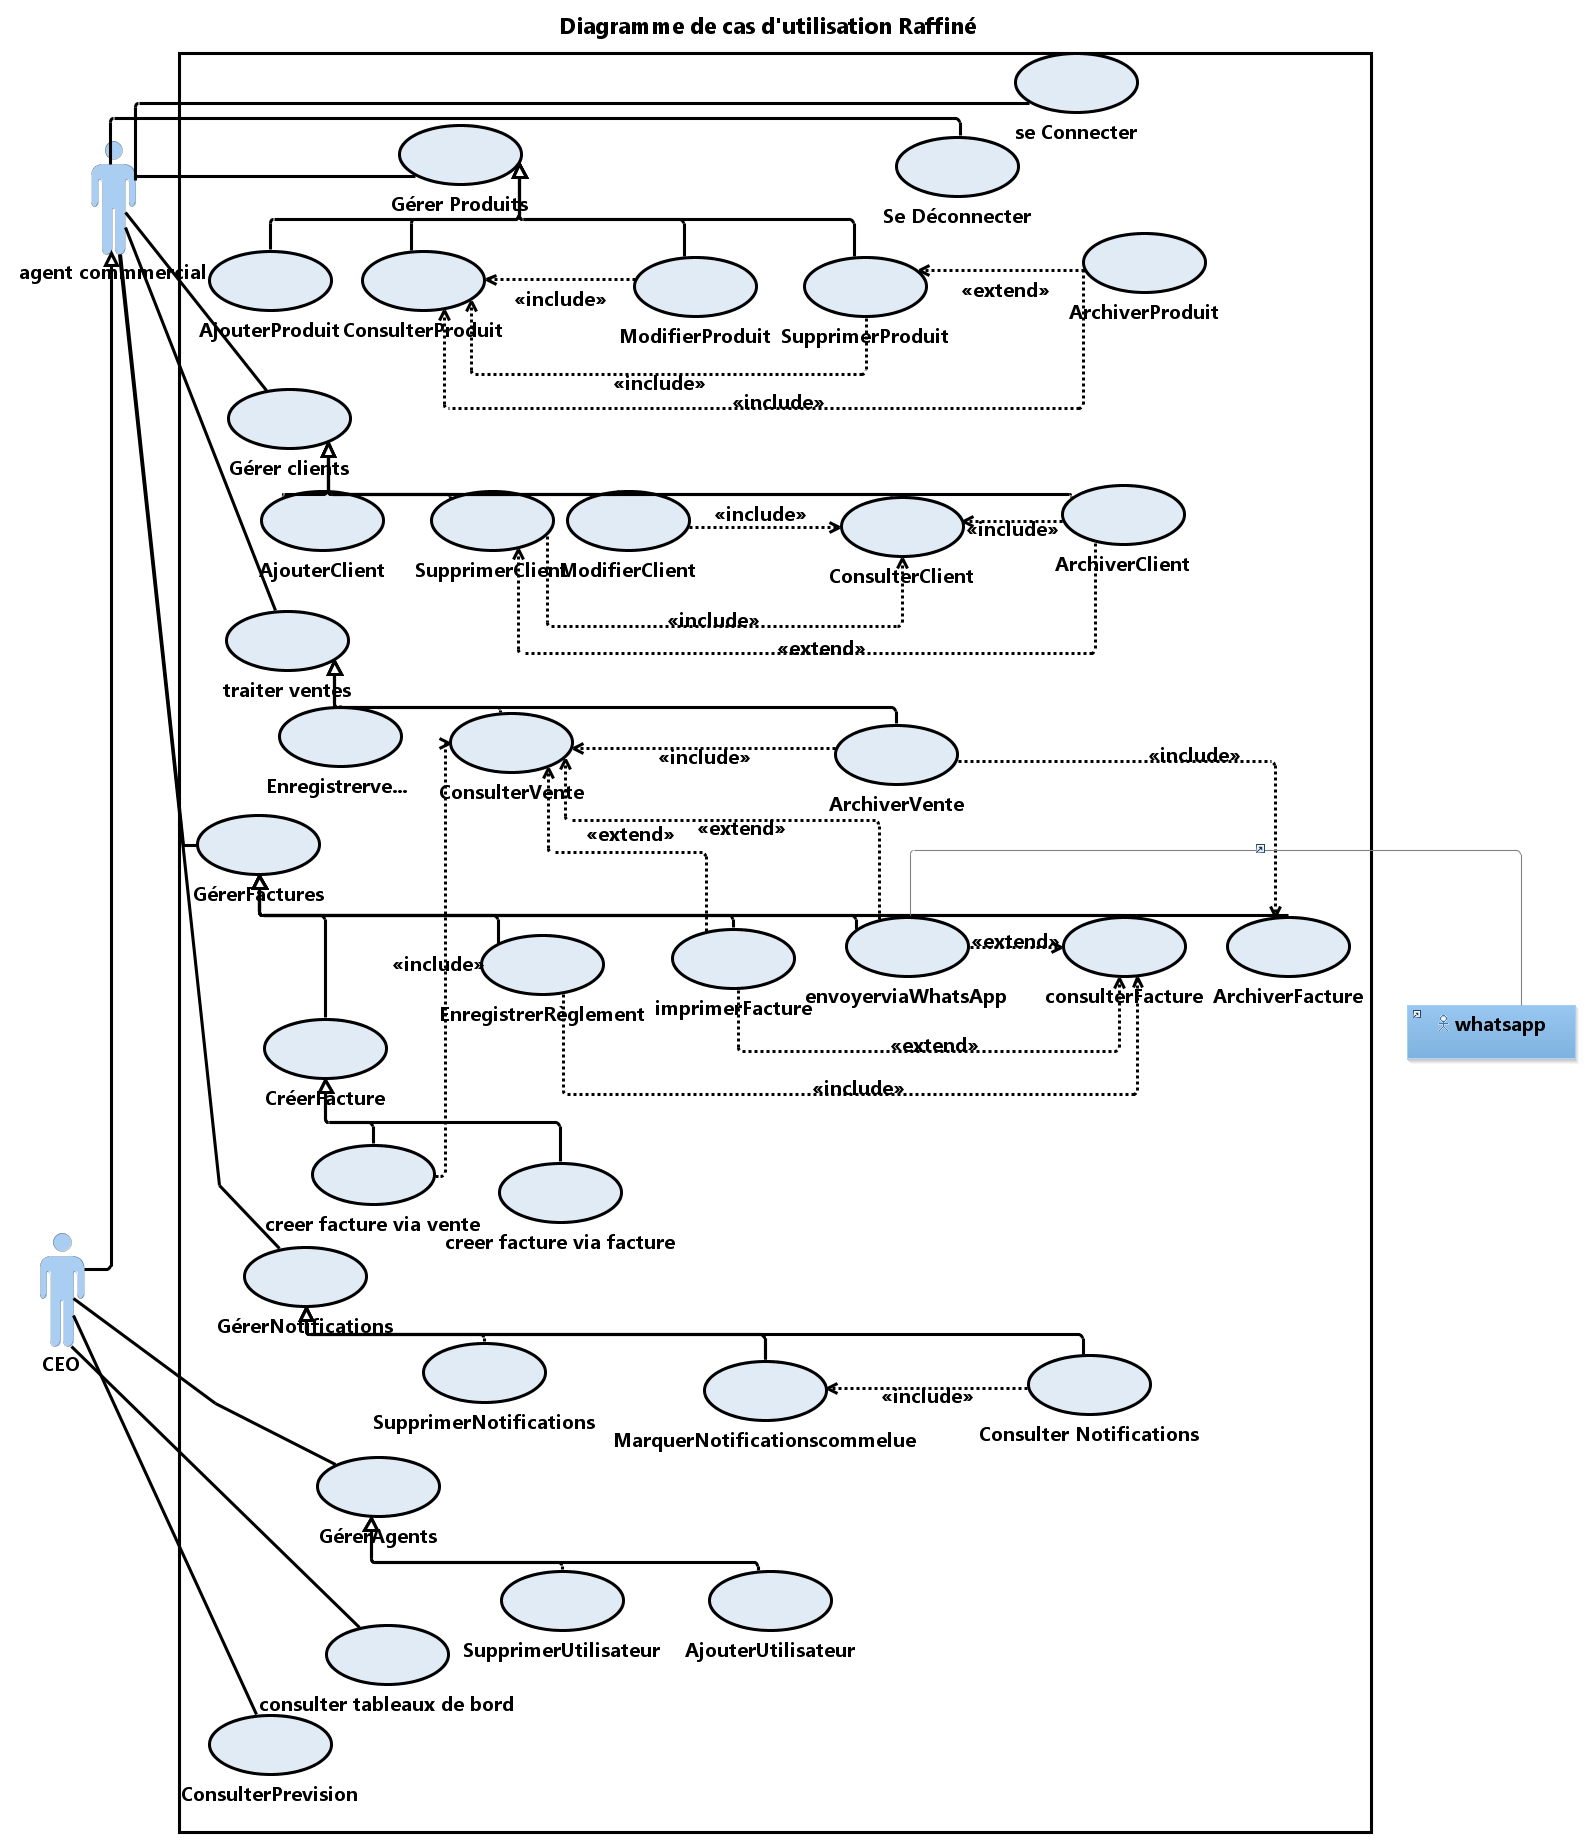
\includegraphics[width=1.3\textwidth, height=0.92\textheight, keepaspectratio]{images/MCU_DiagrammeCasUtilisationRaffiné.png}%
}
  \caption{Diagramme de cas d'utilisation raffiné}
  \label{fig:diagrammeUtilisationRaffine}
\end{figure}

\section*{Conclusion}
À la fin de ce chapitre, nous avons établi une vision claire et ordonnée  sur l'expression des besoins du système.
L'identification des acteurs, les besoins fonctionnels,non fonctionnels et décisionnels a mis en evidence la spécification 
des cas d'utilisation Grâce à leur utilisation, ils ont ensuite été en mesure de modéliser de manière précise les interactions entre les
acteur et le systéme 
Ces éléments sont la base sur laquelle la phase de conception  est présentée dans le chapitre qui suit.

\mychapter{Conception}

\section{Introduction}

Ce chapitre est consacré à la conception de notre systéme . 
Nous commençons par présenter l'architecture logique adoptée. Nous exposons 
ensuite les diagrammes de séquence illustrant les principaux flux d'interactions 
entre les acteurs et le système. Nous présentons par la suite le diagramme de 
classes des entités de notre systéme ,la Conception des Indicateurs Clés de Performances et le  schéma de la base de données, 
afin d'assurer une compréhension claire de la structure des données.

\section{Architecture Logique Adoptée}

Notre application repose sur une architecture \textbf{API RESTful inspirée du patron MVC}. 
Cette architecture permet de séparer clairement les différentes responsabilités du système 
afin de faciliter la maintenance, la sécurité et l’évolution de l’application. 
Elle assure également une communication efficace entre le frontend React et le backend FastAPI.

\subsection{Vue (View)}

La vue représente la partie visible par l’utilisateur. Elle est développée avec React sous 
forme d’une application monopage (SPA). Elle permet la gestion des clients, des produits, 
des ventes et des facturations à travers des interfaces interactives et responsives.

Les composants React communiquent avec le backend via des appels HTTP REST afin de récupérer 
et d’envoyer les données nécessaires. La vue assure également l’affichage du tableau de bord, 
des statistiques, des prévisions ainsi que la génération des documents PDF.

\subsection{Modèle (Model)}

Le modèle représente les différentes entités métier du système telles que :
\textit{Client, Produit, Vente, LigneVente, Facturation, Règlement, Notification et Utilisateur}.

Il assure la gestion et la persistance des données dans la base SQLite grâce à SQLAlchemy. 
Le modèle définit également les relations entre les entités ainsi que les contraintes de 
chaque champ afin de garantir l’intégrité des données.

\subsection{Contrôleur (Controller)}

Le contrôleur constitue la partie centrale du traitement des opérations métier. 
Il est composé principalement des routes et des services.

\begin{itemize}
    \item Les \textbf{routes} reçoivent les requêtes provenant du frontend, appliquent 
    l’authentification JWT ainsi que le contrôle d’accès par rôle, puis transmettent 
    les traitements aux services concernés.

    \item Les \textbf{services} regroupent toute la logique métier du système : 
    vérification du stock, gestion des ventes, calcul des montants, génération des 
    références, création des notifications automatiques et préparation des données 
    envoyées au frontend.
\end{itemize}

\begin{figure}[H]
    \centering
    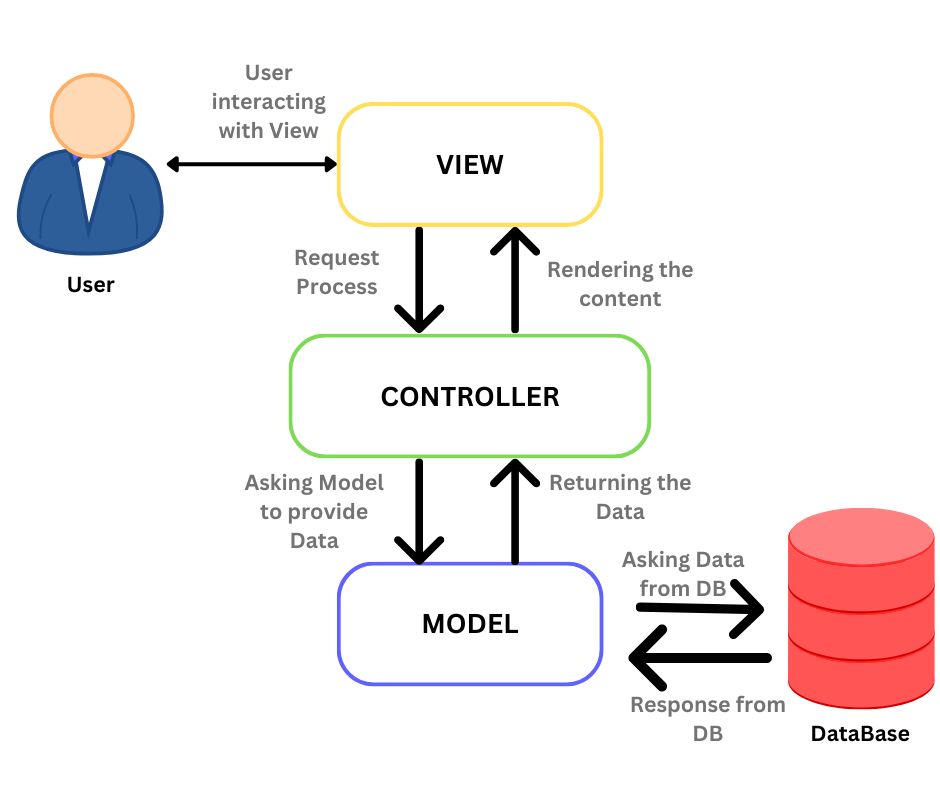
\includegraphics[width=0.9\textwidth]{images/1_eqghG-tH1flMjAOFcsOjIQ.png}
    \caption{Architecture MVC adoptée dans le système}
    \label{fig:mvc_architecture}
\end{figure}

\newpage
\section{Conception du Cas D'utilisation Se Connecter}

\needspace{0.88\textheight}
\subsection{Traçabilité MCU/MC pour le Cas D'utilisation Se Connecter}

\begin{figure}[H]
  \centering
  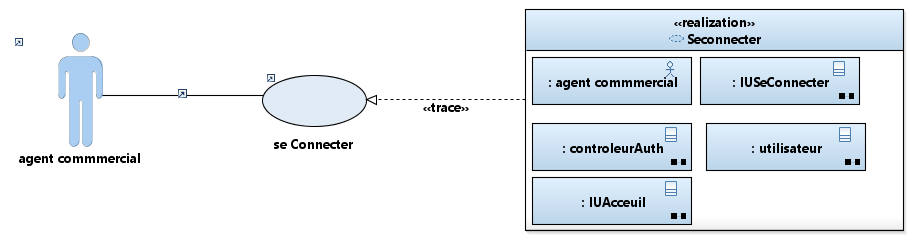
\includegraphics[width=1\textwidth]{images/MC1_DiagrammeFormatConnecter.png}
  \caption{Traçabilité MCU/MC pour le cas d'utilisation Se Connecter}
\end{figure}

Cette traçabilité montre la réalisation du cas d'utilisation à travers les différents objets collaborant dans l'architecture du système.

Les classes impliquées dans ce diagramme sont les suivantes :

\begin{itemize}[leftmargin=2em, topsep=4pt, itemsep=4pt]
  \item \textbf{Agent Commercial :} l'utilisateur qui initie le processus de connexion
  \item \textbf{IUSeConnecter :} l'interface qui permet la saisie des identifiants de connexion
  \item \textbf{IUAccueil :} l'interface principale affichée à l'utilisateur après une connexion réussie
  \item \textbf{ControleurAuth :} l'intermédiaire entre l'interface de connexion et l'entité utilisateur
  \item \textbf{Utilisateur :} l'entité du système qui contient les données relatives aux utilisateurs et les traitements à appliquer
\end{itemize}



\needspace{0.88\textheight}
\subsection{Diagramme de Séquence du Cas D'utilisation Se Connecter}

\begin{figure}[H]
  \centering
  \makebox[\textwidth][c]{%
    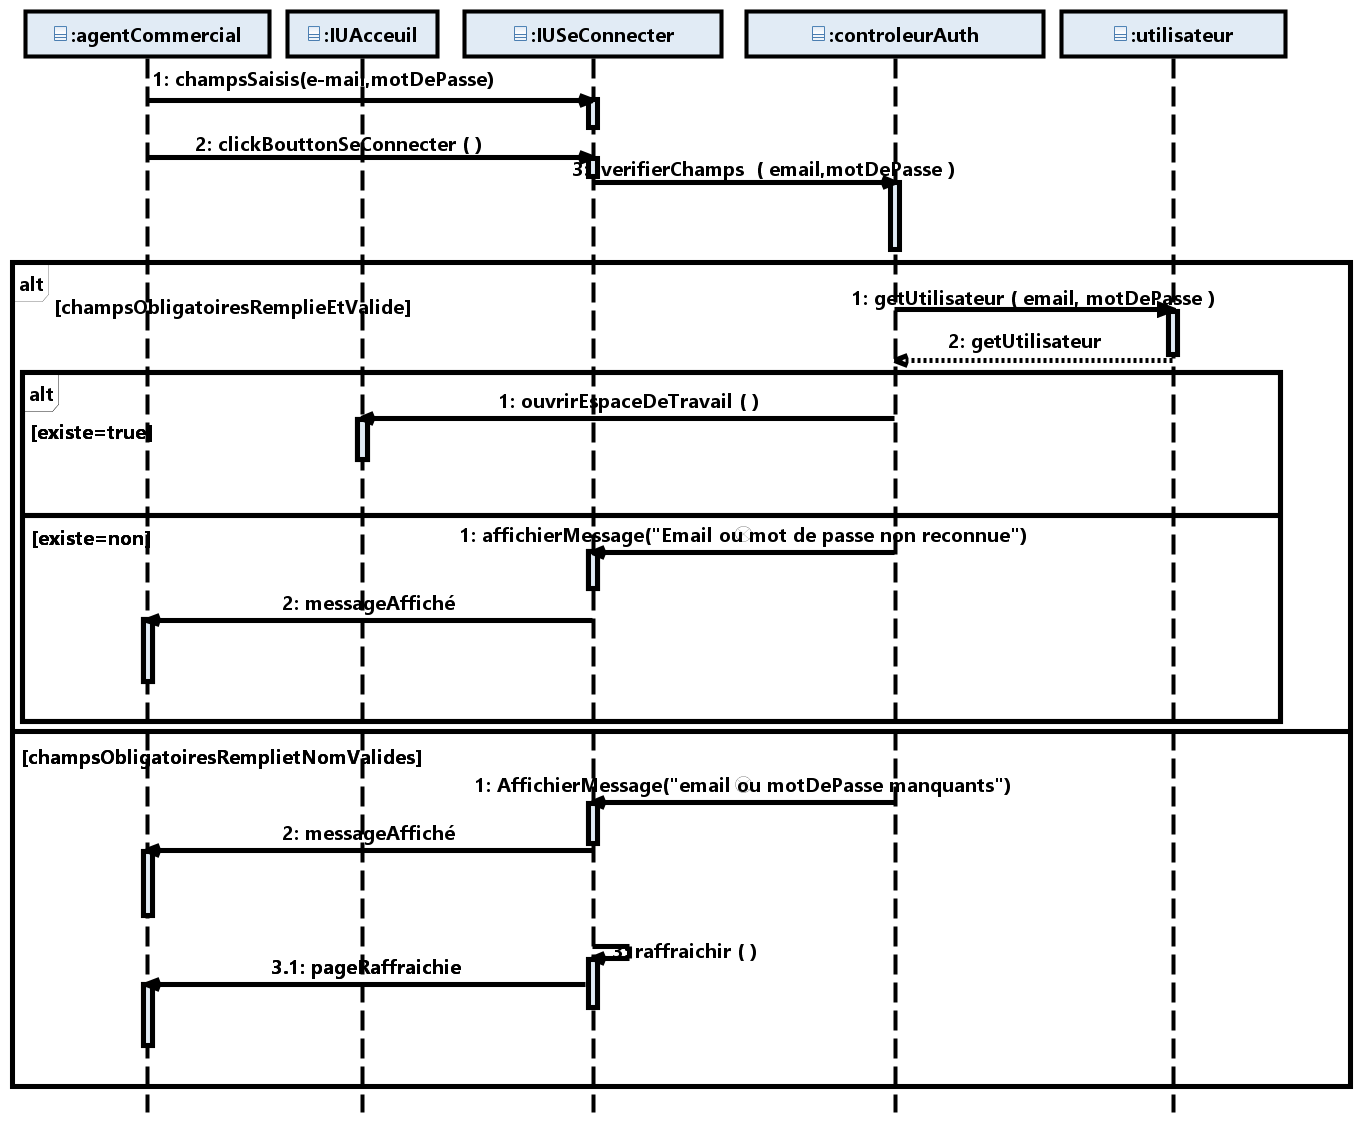
\includegraphics[width=1.15\textwidth, height=0.78\textheight]{images/MC_DiagrammeSéquenceSeConnecter_1.png}%
  }
  \caption{Diagramme de séquence pour le cas d'utilisation Se Connecter}
  \label{fig:seqConnecter}
\end{figure}
À noter que le CEO utilise également ce cas d'utilisation en suivant le même processus que l'agent commercial.
\needspace{0.88\textheight}
\subsection{Diagramme de Classe du Cas D'utilisation Se Connecter}

\begin{figure}[H]
  \centering
  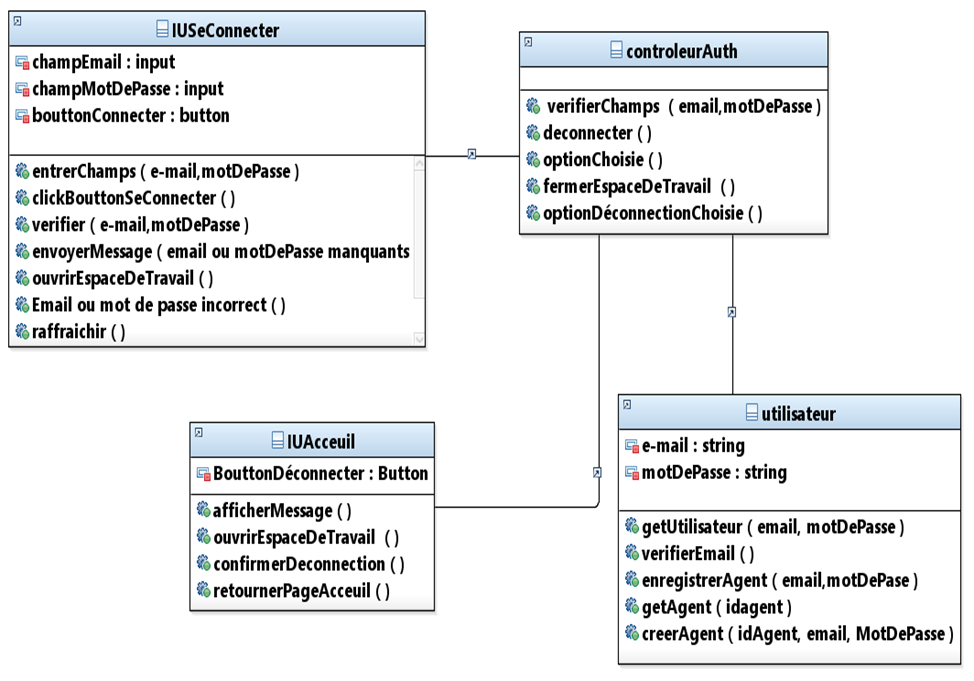
\includegraphics[width=0.75\textwidth, height=0.50\textheight, keepaspectratio]{images/classeConnecter.png}
  \caption{Diagramme de classe pour le cas d'utilisation Se Connecter}
  \label{fig:classeConnecter}
\end{figure}

\newpage

\section{Conception du Cas D'utilisation Se Déconnecter}

\needspace{0.88\textheight}
\subsection{Traçabilité MCU/MC pour le Cas D'utilisation Se Déconnecter}

\begin{figure}[H]
  \centering
  \makebox[\textwidth][c]{%
    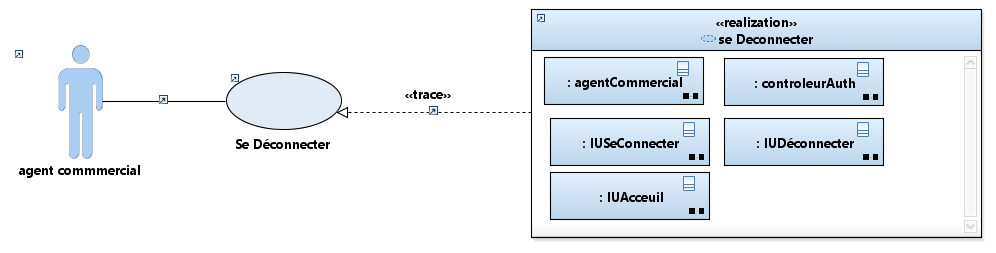
\includegraphics[width=1.1\textwidth, height=0.25\textheight]{images/MC1_tracabiltéMCUMCseDéconnecter.png}%
  }
  \caption{Traçabilité MCU/MC pour le cas d'utilisation Se Déconnecter}
\end{figure}

Cette traçabilité montre quels sont les objets instance de classe participant a la réalisation du cas d'utilisation Se Déconnecter

L'acteur et Les classes impliquées dans cette réalisation sont les suivants :

\begin{itemize}[leftmargin=2em, topsep=4pt, itemsep=4pt]
  \item \textbf{Agent Commercial :} l'utilisateur qui initie le processus de déconnexion
  \item \textbf{IUDeconnecter :} l'interface qui permet à l'utilisateur de confirmer sa déconnexion
  \item \textbf{IUSeConnecter :} l'interface vers laquelle l'utilisateur est redirigé après la déconnexion
  \item \textbf{IUAccueil :} l'interface depuis laquelle l'utilisateur déclenche la déconnexion
  \item \textbf{ControleurAuth :} responsable du traitement et de la validation de la déconnexion
\end{itemize}

À noter que le CEO utilise également ce cas d'utilisation en suivant le même processus que l'agent commercial.

\needspace{0.88\textheight}
\subsection{Diagramme de Séquence du Cas D'utilisation Se Déconnecter}

\begin{figure}[H]
  \centering
  \makebox[\textwidth][c]{%
    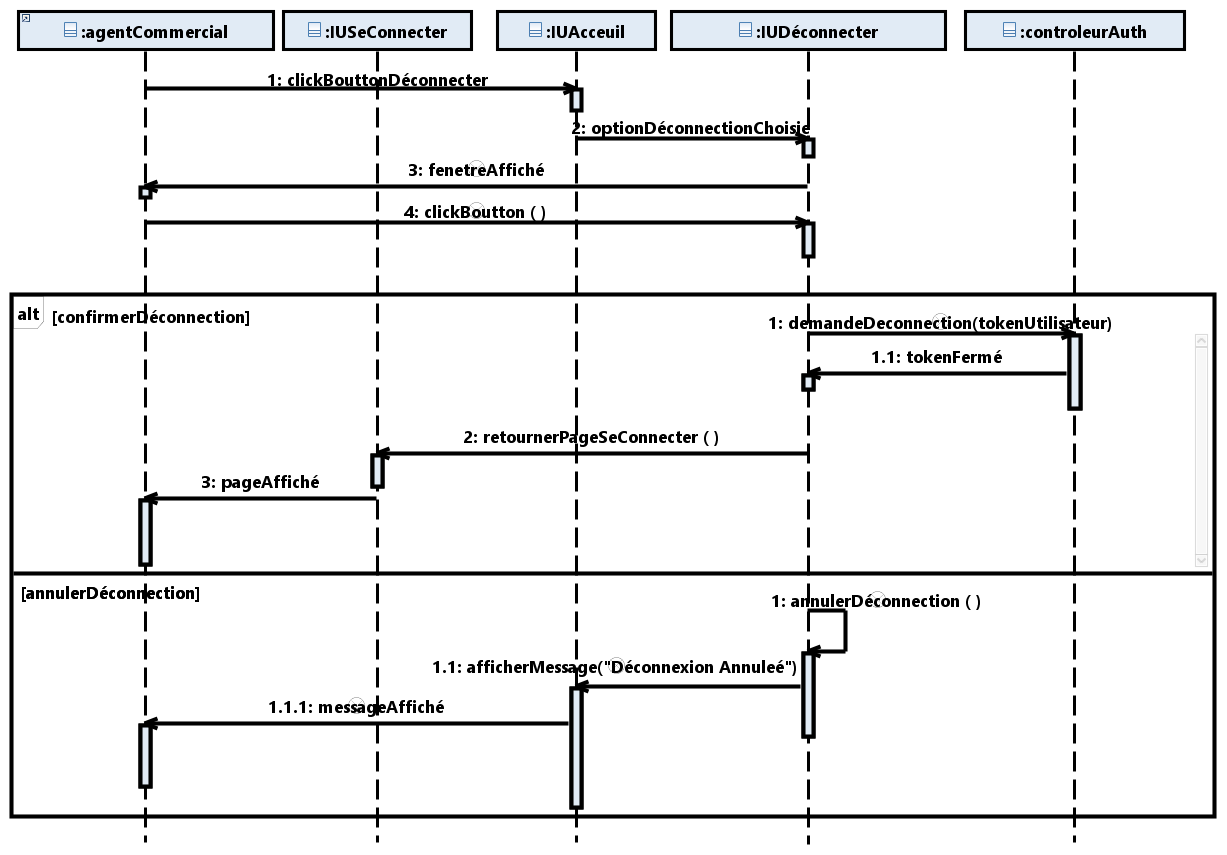
\includegraphics[width=1.15\textwidth, height=0.78\textheight]{images/MC_DiagrammeSéquenceSeDéconnecter.png}%
  }
  \caption{Diagramme de séquence pour le cas d'utilisation Se Déconnecter}
  \label{fig:seqDeconnecter}
\end{figure}

\needspace{0.88\textheight}
\subsection{Diagramme de Classe du Cas D'utilisation Se Déconnecter}

\begin{figure}[H]
  \centering
  \makebox[\textwidth][c]{%
    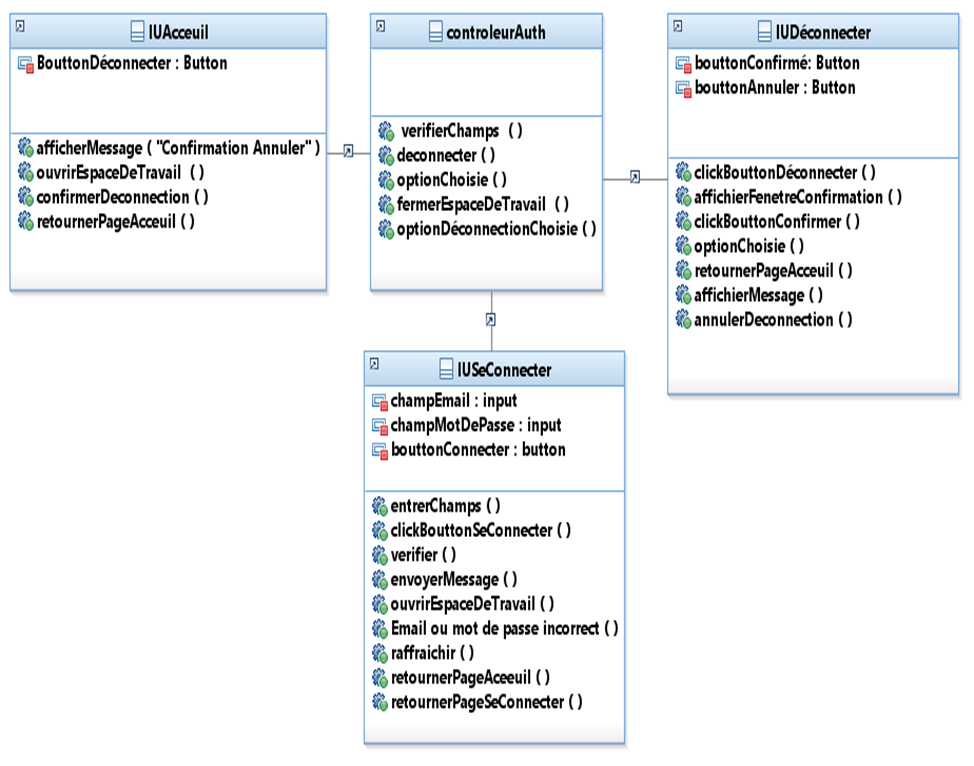
\includegraphics[width=1.05\textwidth, height=0.55\textheight]{images/classedeconnecter.png}%
  }
  \caption{Diagramme de classe pour le cas d'utilisation Se Déconnecter}
  \label{fig:classeDeconnecter}
\end{figure}
\newpage

\section{Conception des Cas D'utilisation Gérer Agents}

\needspace{0.88\textheight}
\subsection{Traçabilité MCU/MC pour le Cas D'utilisation Gérer Agents}

\begin{figure}[H]
  \centering
  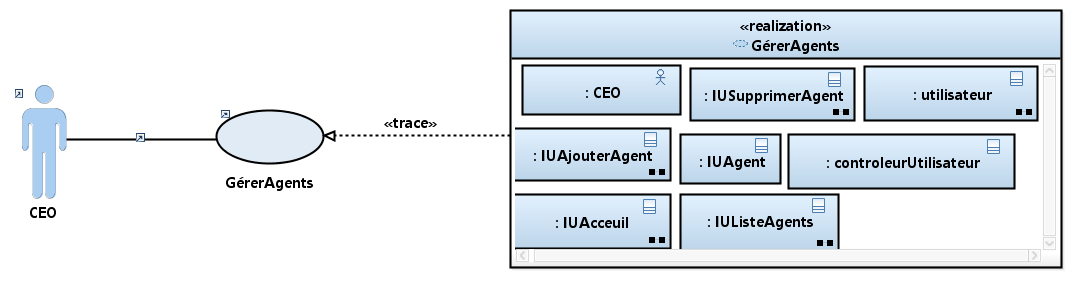
\includegraphics[width=\textwidth]{images/MC1_tracabilitéMCUMCGérerUtilisateurs_1.png}
  \caption{Traçabilité MCU/MC pour le cas d'utilisation Gérer Agents}
\end{figure}

Cette traçabilité montre quels sont les objets instance participant à la réalisation de la classe du cas d'utilisation gérer Agents.
L'acteur et Les classes impliquées dans cette réalisation sont les suivants :

\begin{itemize}[leftmargin=2em, topsep=4pt, itemsep=4pt]
  \item \textbf{CEO :} l'acteur qui initie les opérations de gestion des utilisateurs
  \item \textbf{IUAccueil :} l'interface principale depuis laquelle le CEO accède à la page de gestion des agents
  \item \textbf{IUAgent :} l'interface principales pour gérer les agents
  \item \textbf{IUAjouterAgent :} l'interface qui permet au CEO d'ajouter un nouvel utilisateur en définissant son email, mot de passe et rôle
  \item \textbf{IUSupprimerAgent :} l'interface qui permet au CEO de confirmer la suppression d'un agent du système
  \item \textbf{IUListeAgent :} l'interface qui affiche la liste des utilisateurs du système et permet au CEO de supprimer un agent
  \item \textbf{ControleurUtilisateur :} permet de gérer les flux de contrôle entre l'interface et l'entité
  \item \textbf{Utilisateur :} l'entité du système qui contient les données relative aux agents et les traitements métiers associés
\end{itemize}

\needspace{0.88\textheight}
\subsection{Diagramme de Séquence du Cas D'utilisation Ajouter Agent}

\begin{figure}[H]
  \centering
  \makebox[\textwidth][c]{%
    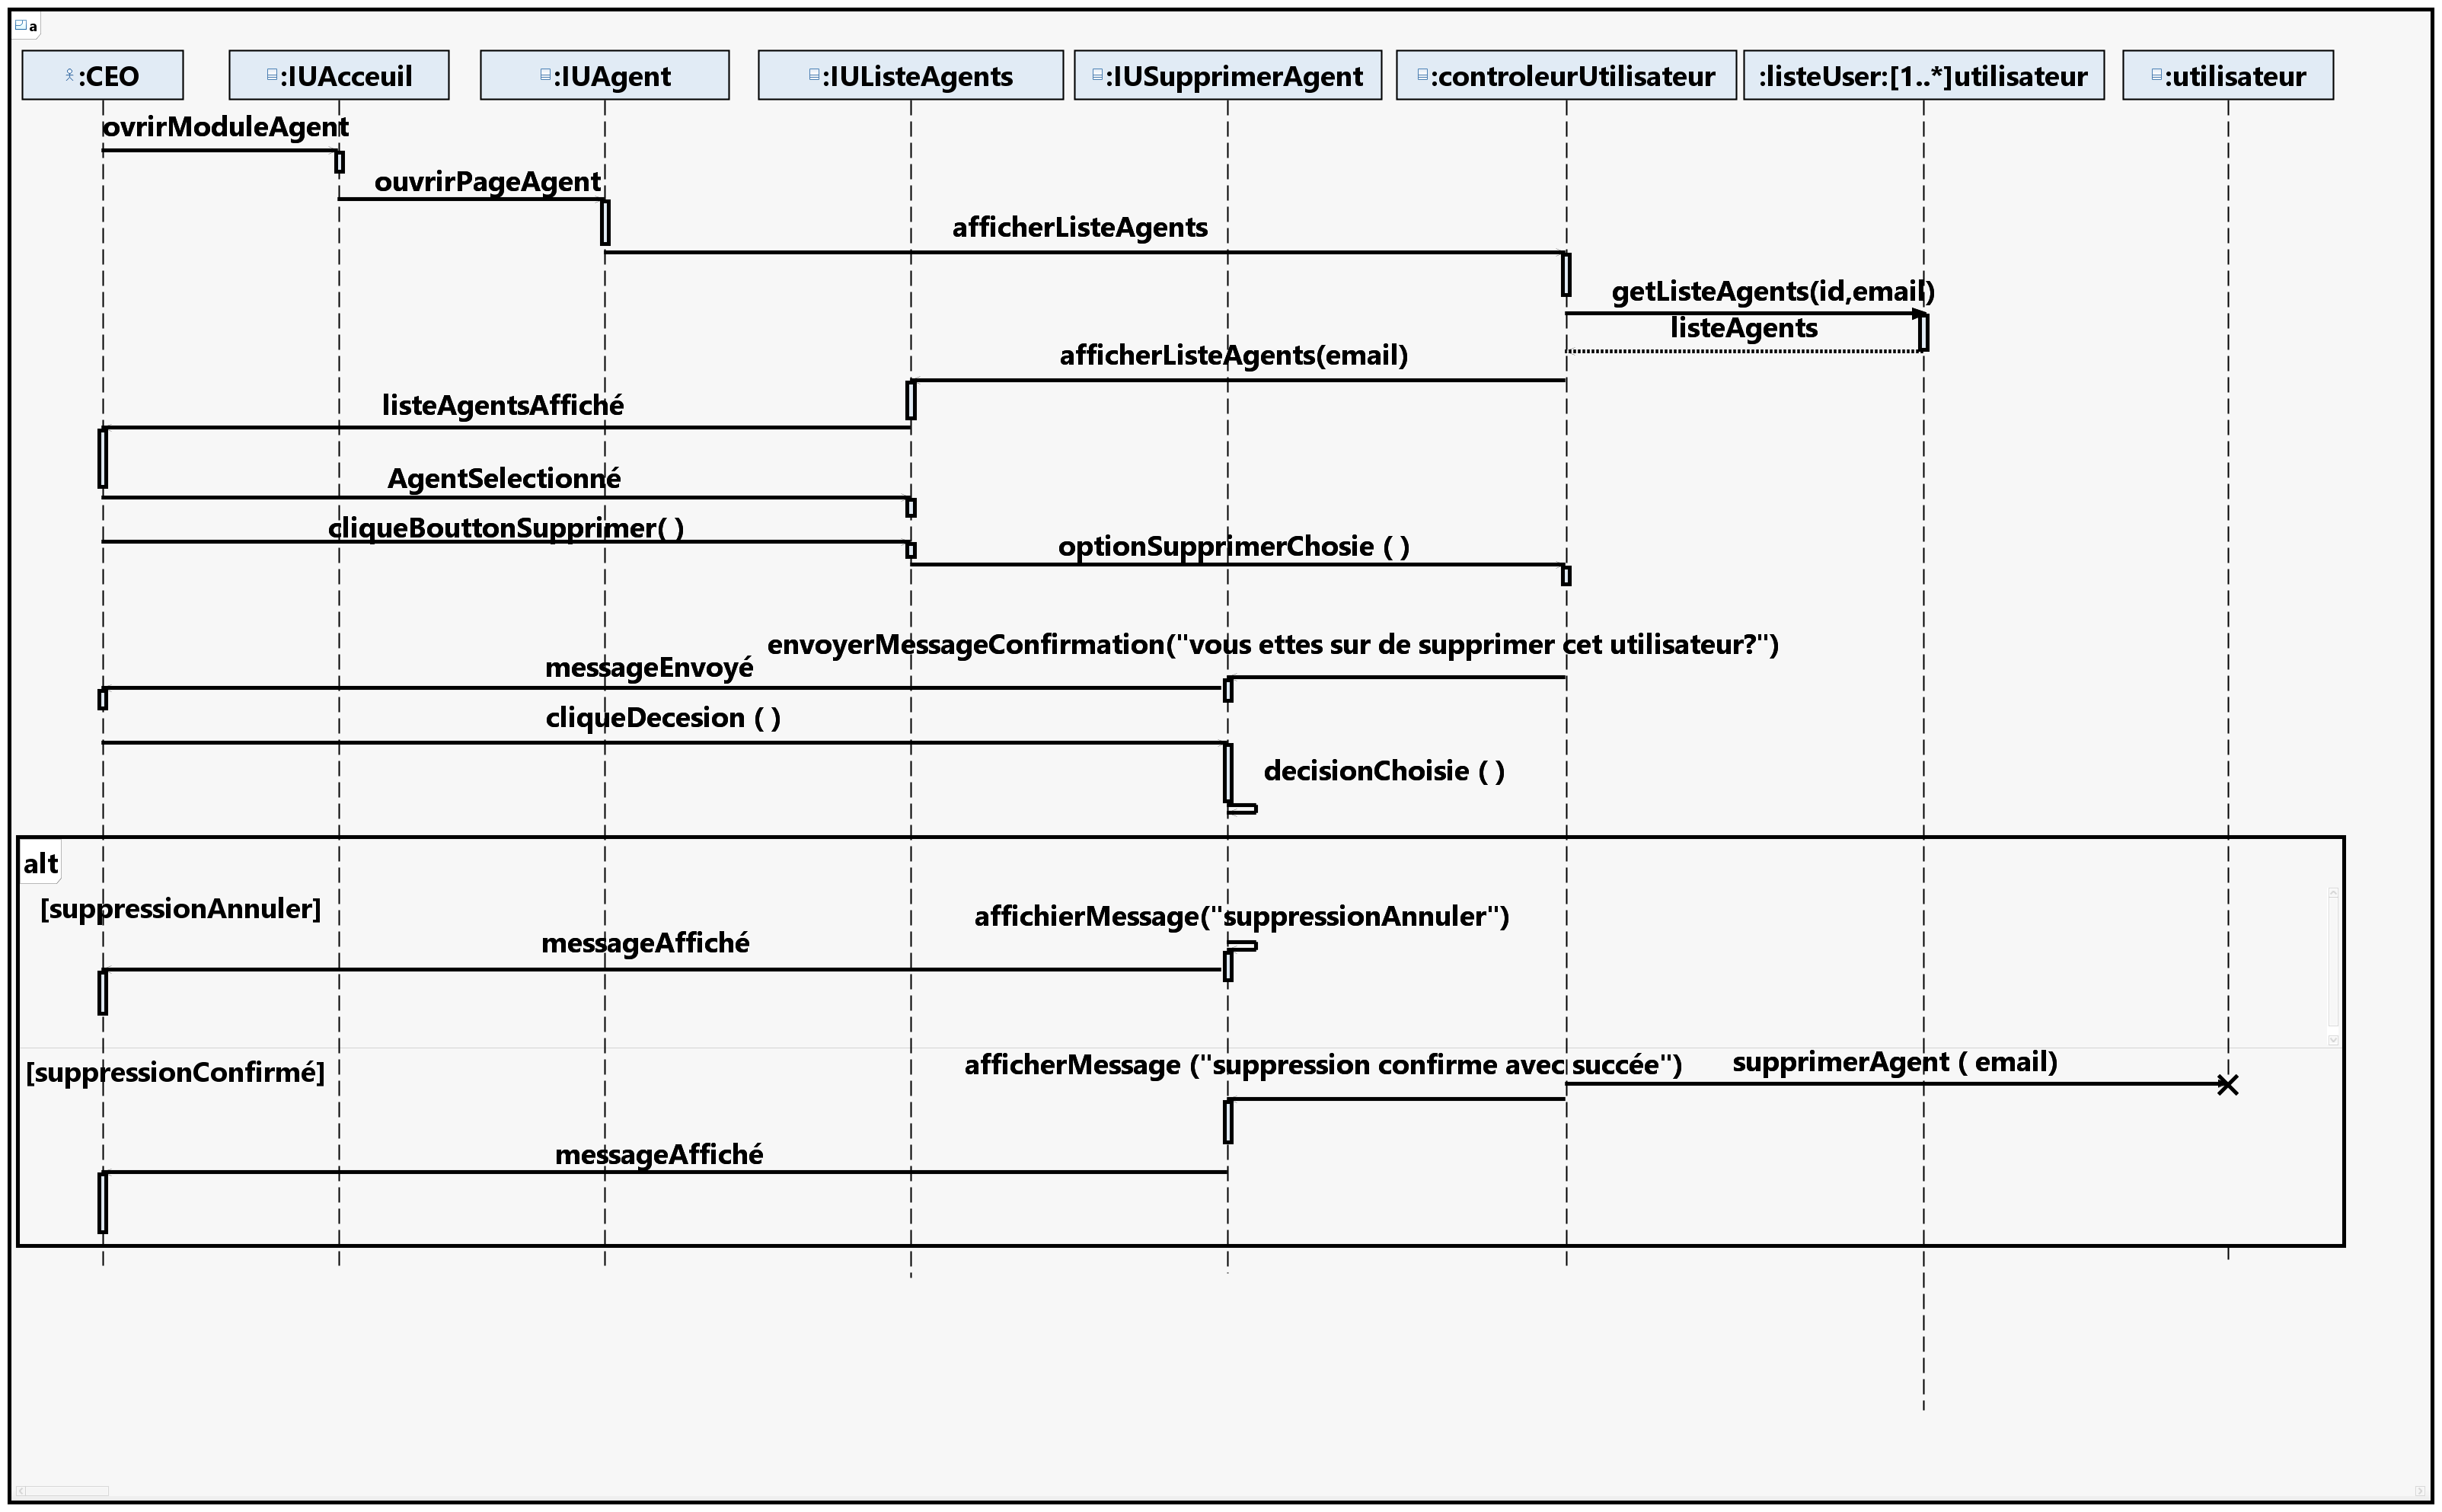
\includegraphics[width=1.15\textwidth, height=0.78\textheight]{images/MC1_DiagrammeSéquenceSupprimerUtilisateur_1.png}%
  }
  \caption{Diagramme de séquence pour le cas d'utilisation Ajouter Agent}
  \label{fig:seqAjouterAgent}
\end{figure}

\needspace{0.88\textheight}
\subsection{Diagramme de Séquence du Cas D'utilisation Supprimer Agent}

\begin{figure}[H]
  \centering
  \makebox[\textwidth][c]{%
    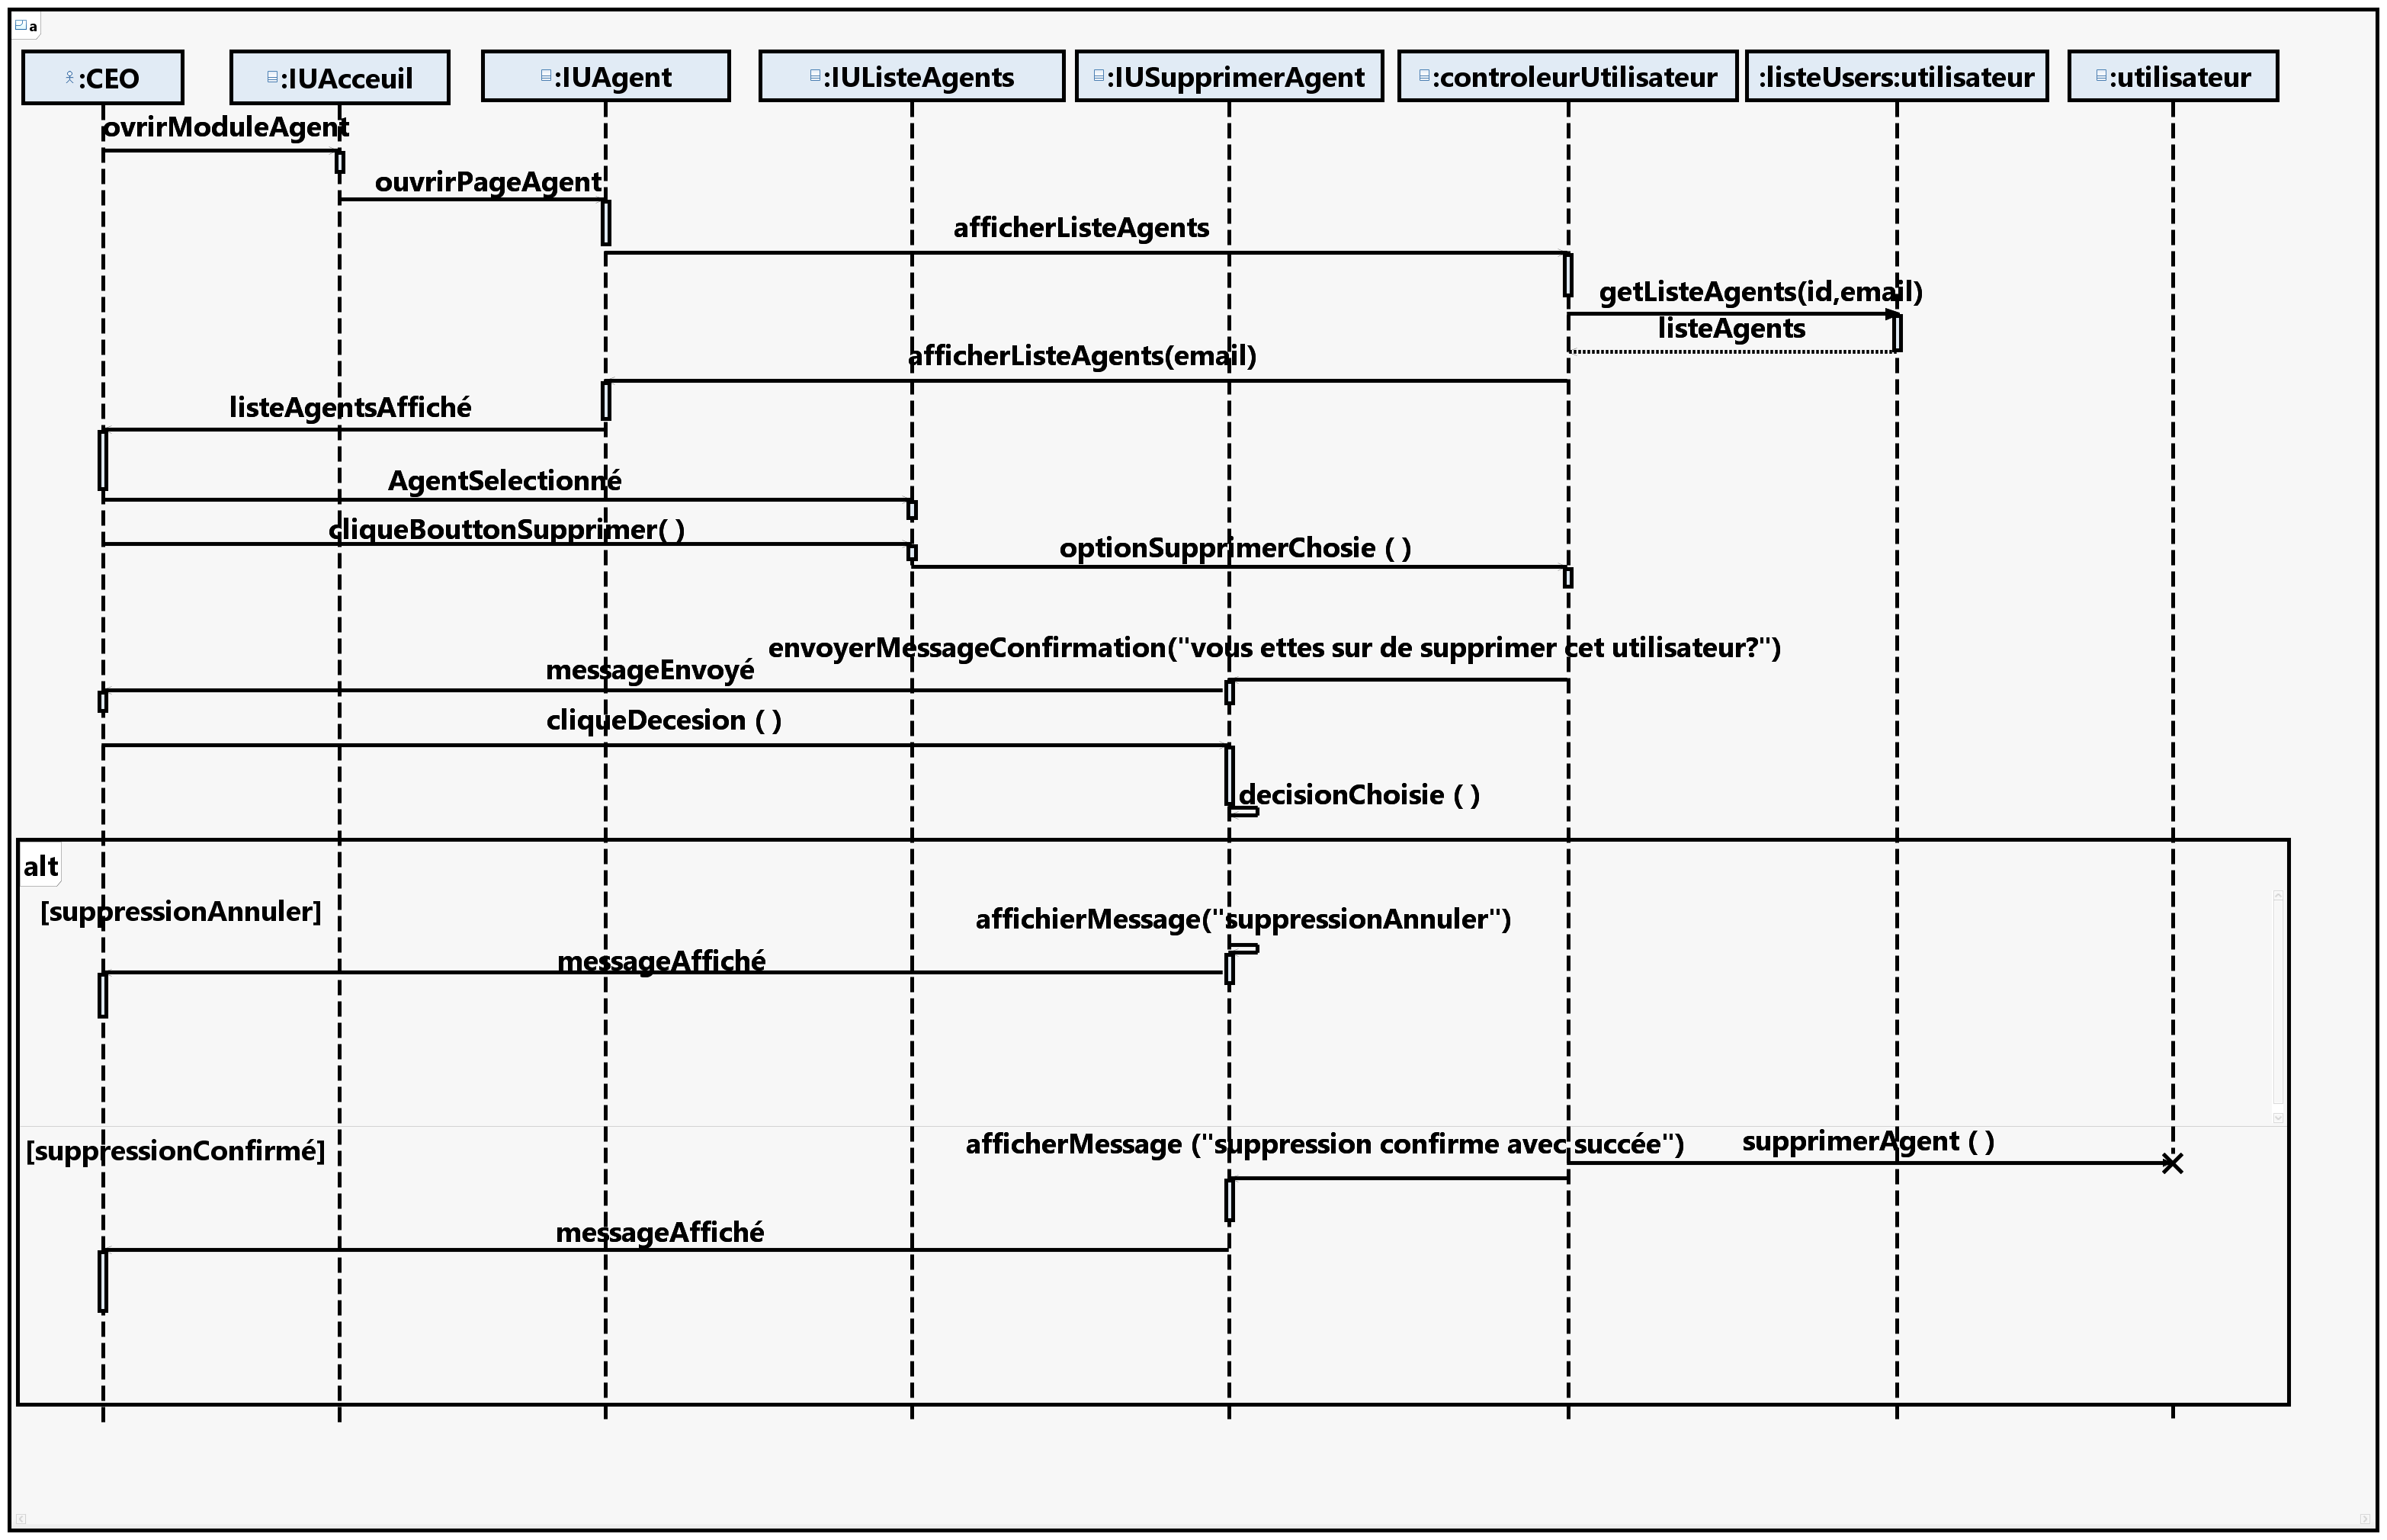
\includegraphics[width=1.15\textwidth, height=0.78\textheight]{images/MC1_DiagrammeSéquenceSupprimerUtilisateur.png}%
  }
  \caption{Diagramme de séquence pour le cas d'utilisation Supprimer Agent}
  \label{fig:seqSupprimerAgent}
\end{figure}
Il est à noter que le CEO peut également effectuer les mêmes opérations de gestion des Agents
\needspace{0.88\textheight}
\subsection{Diagramme de Classe du Cas D'utilisation Gérer Agents}

\begin{figure}[H]
  \centering
  \makebox[\textwidth][c]{%
    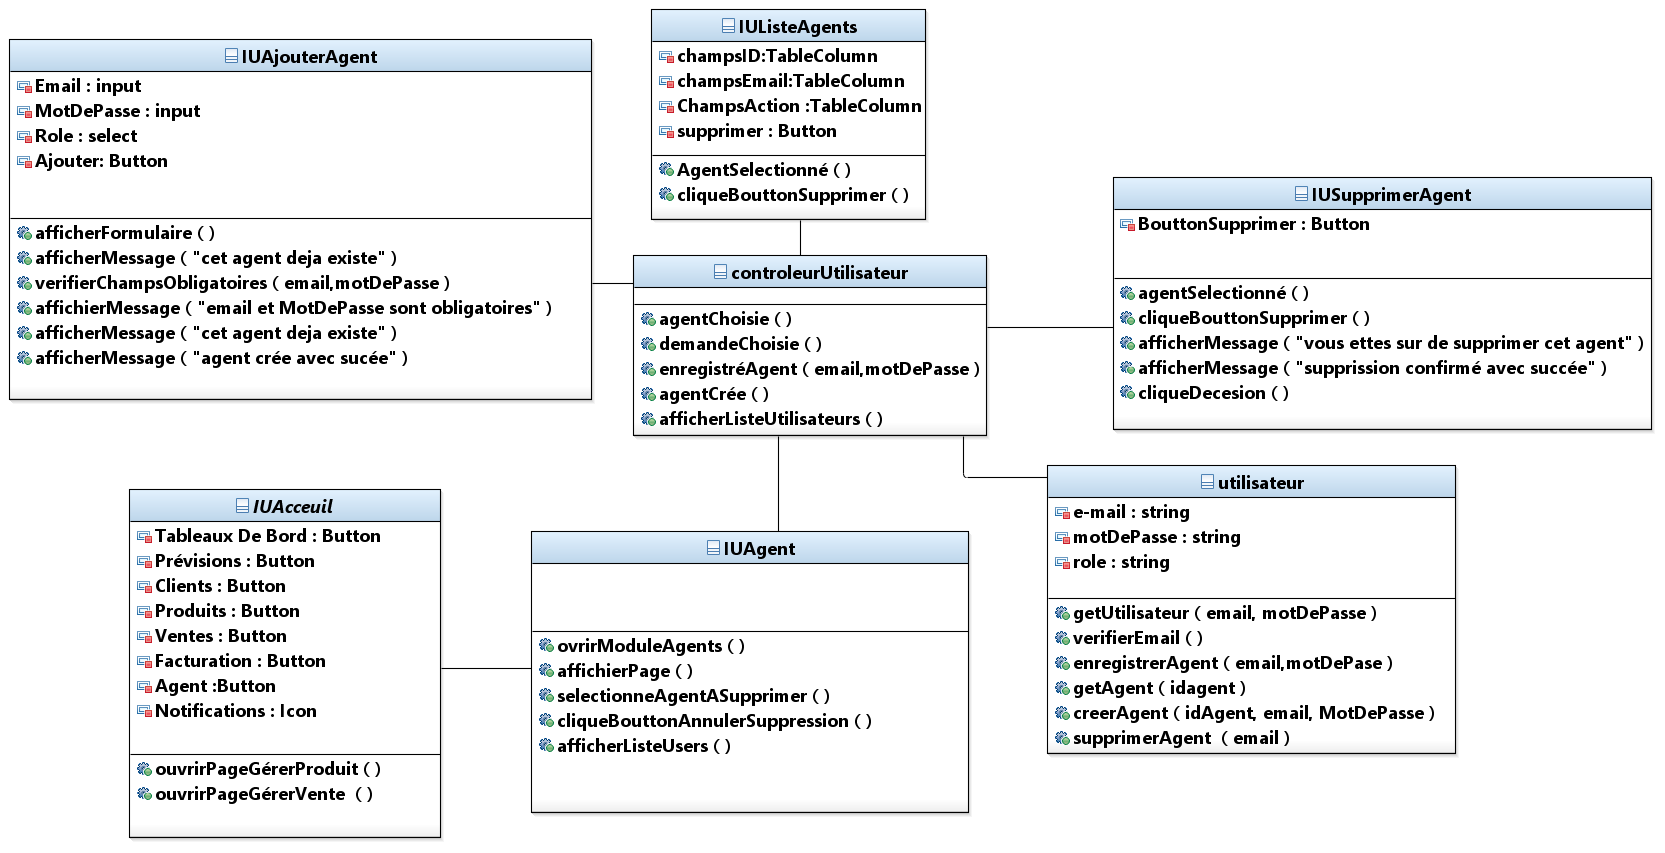
\includegraphics[width=0.95\textwidth, height=0.78\textheight]{images/MC1_DiagrammeClasseGérerUtilisateurs_1.png}%
  }
  \caption{Diagramme de classe pour le cas d'utilisation Gérer Agents}
  \label{fig:classeAgents}
\end{figure}
\newpage

\section{Conception des Cas D'utilisation Gérer Produits}
\needspace{0.88\textheight}
\subsection{Traçabilité MCU/MC pour le Cas D'utilisation Gérer Produits}

\begin{figure}[H]
  \centering
  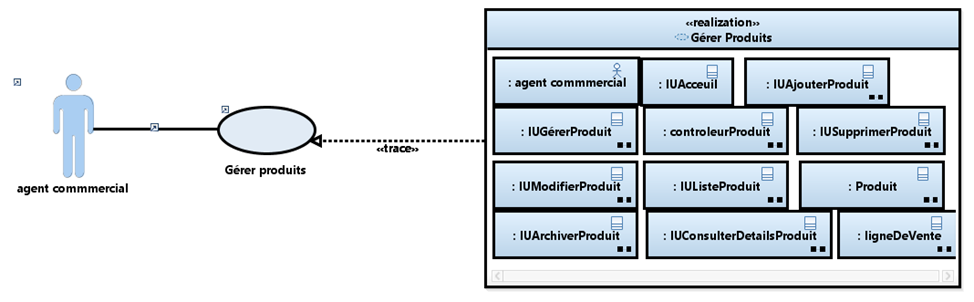
\includegraphics[width=\textwidth]{images/mcumcpoduit.png}
  \caption{Traçabilité MCU/MC pour le cas d'utilisation Gérer Produits}
\end{figure}

Cette traçabilité montre quels sont les objets instances  de classe participant à la réalisation du cas d'utilisation Gérer Produits.

L'acteur et Les classes impliquées dans ce diagramme sont les suivantes :

\begin{itemize}[leftmargin=2em, topsep=4pt, itemsep=4pt]
  \item \textbf{Agent Commercial :} l'acteur qui initie les opérations de gestion des produits
  \item \textbf{IUGérerProduit :} l'interface principale qui affiche les options de gestion des produits avec les options de recherche et de filtrage
  \item \textbf{IUAccueil :} l'interface principale depuis laquelle l'agent accède à la page de gestion des produits
  \item \textbf{IUAjouterProduit :} l'interface qui permet à l'agent commercial d'ajouter un nouveau produit en définissant son nom, catégorie, prix unitaire et stock
  \item \textbf{IUModifierProduit :} l'interface qui permet à l'agent commercial de modifier les informations d'un produit existant
  \item \textbf{IUSupprimerProduit :} l'interface qui permet à l'agent commercial de confirmer la suppression d'un produit du système
  \item \textbf{IUArchiverProduit :} l'interface qui permet à l'agent commercial de confirmer l'archivage d'un produit
  \item \textbf{IUConsulterDetailsProduit :} l'interface qui permet à l'agent commercial de visualiser les détails d'un produit sélectionné
  \newpage
  \item \textbf{IUListeProduit :} l'interface qui affiche la liste des produits
  \item \textbf{ControleurProduit :} permet de gérer les flux de contrôle entre l'interface utilisateur et l'entité produit
  \item \textbf{Produit :} la classe du système qui contient les données  relatives aux produits et les traitements métier associés
  \item \textbf{LigneDeVente :} la classe du système qui contient les données et les traitements métier relatives aux produits liés à une vente
\end{itemize}


\needspace{0.88\textheight}
\subsection{Diagramme de Séquence du Cas D'utilisation Ajouter Produit}

\begin{figure}[H]
  \centering
  \makebox[\textwidth][c]{%
    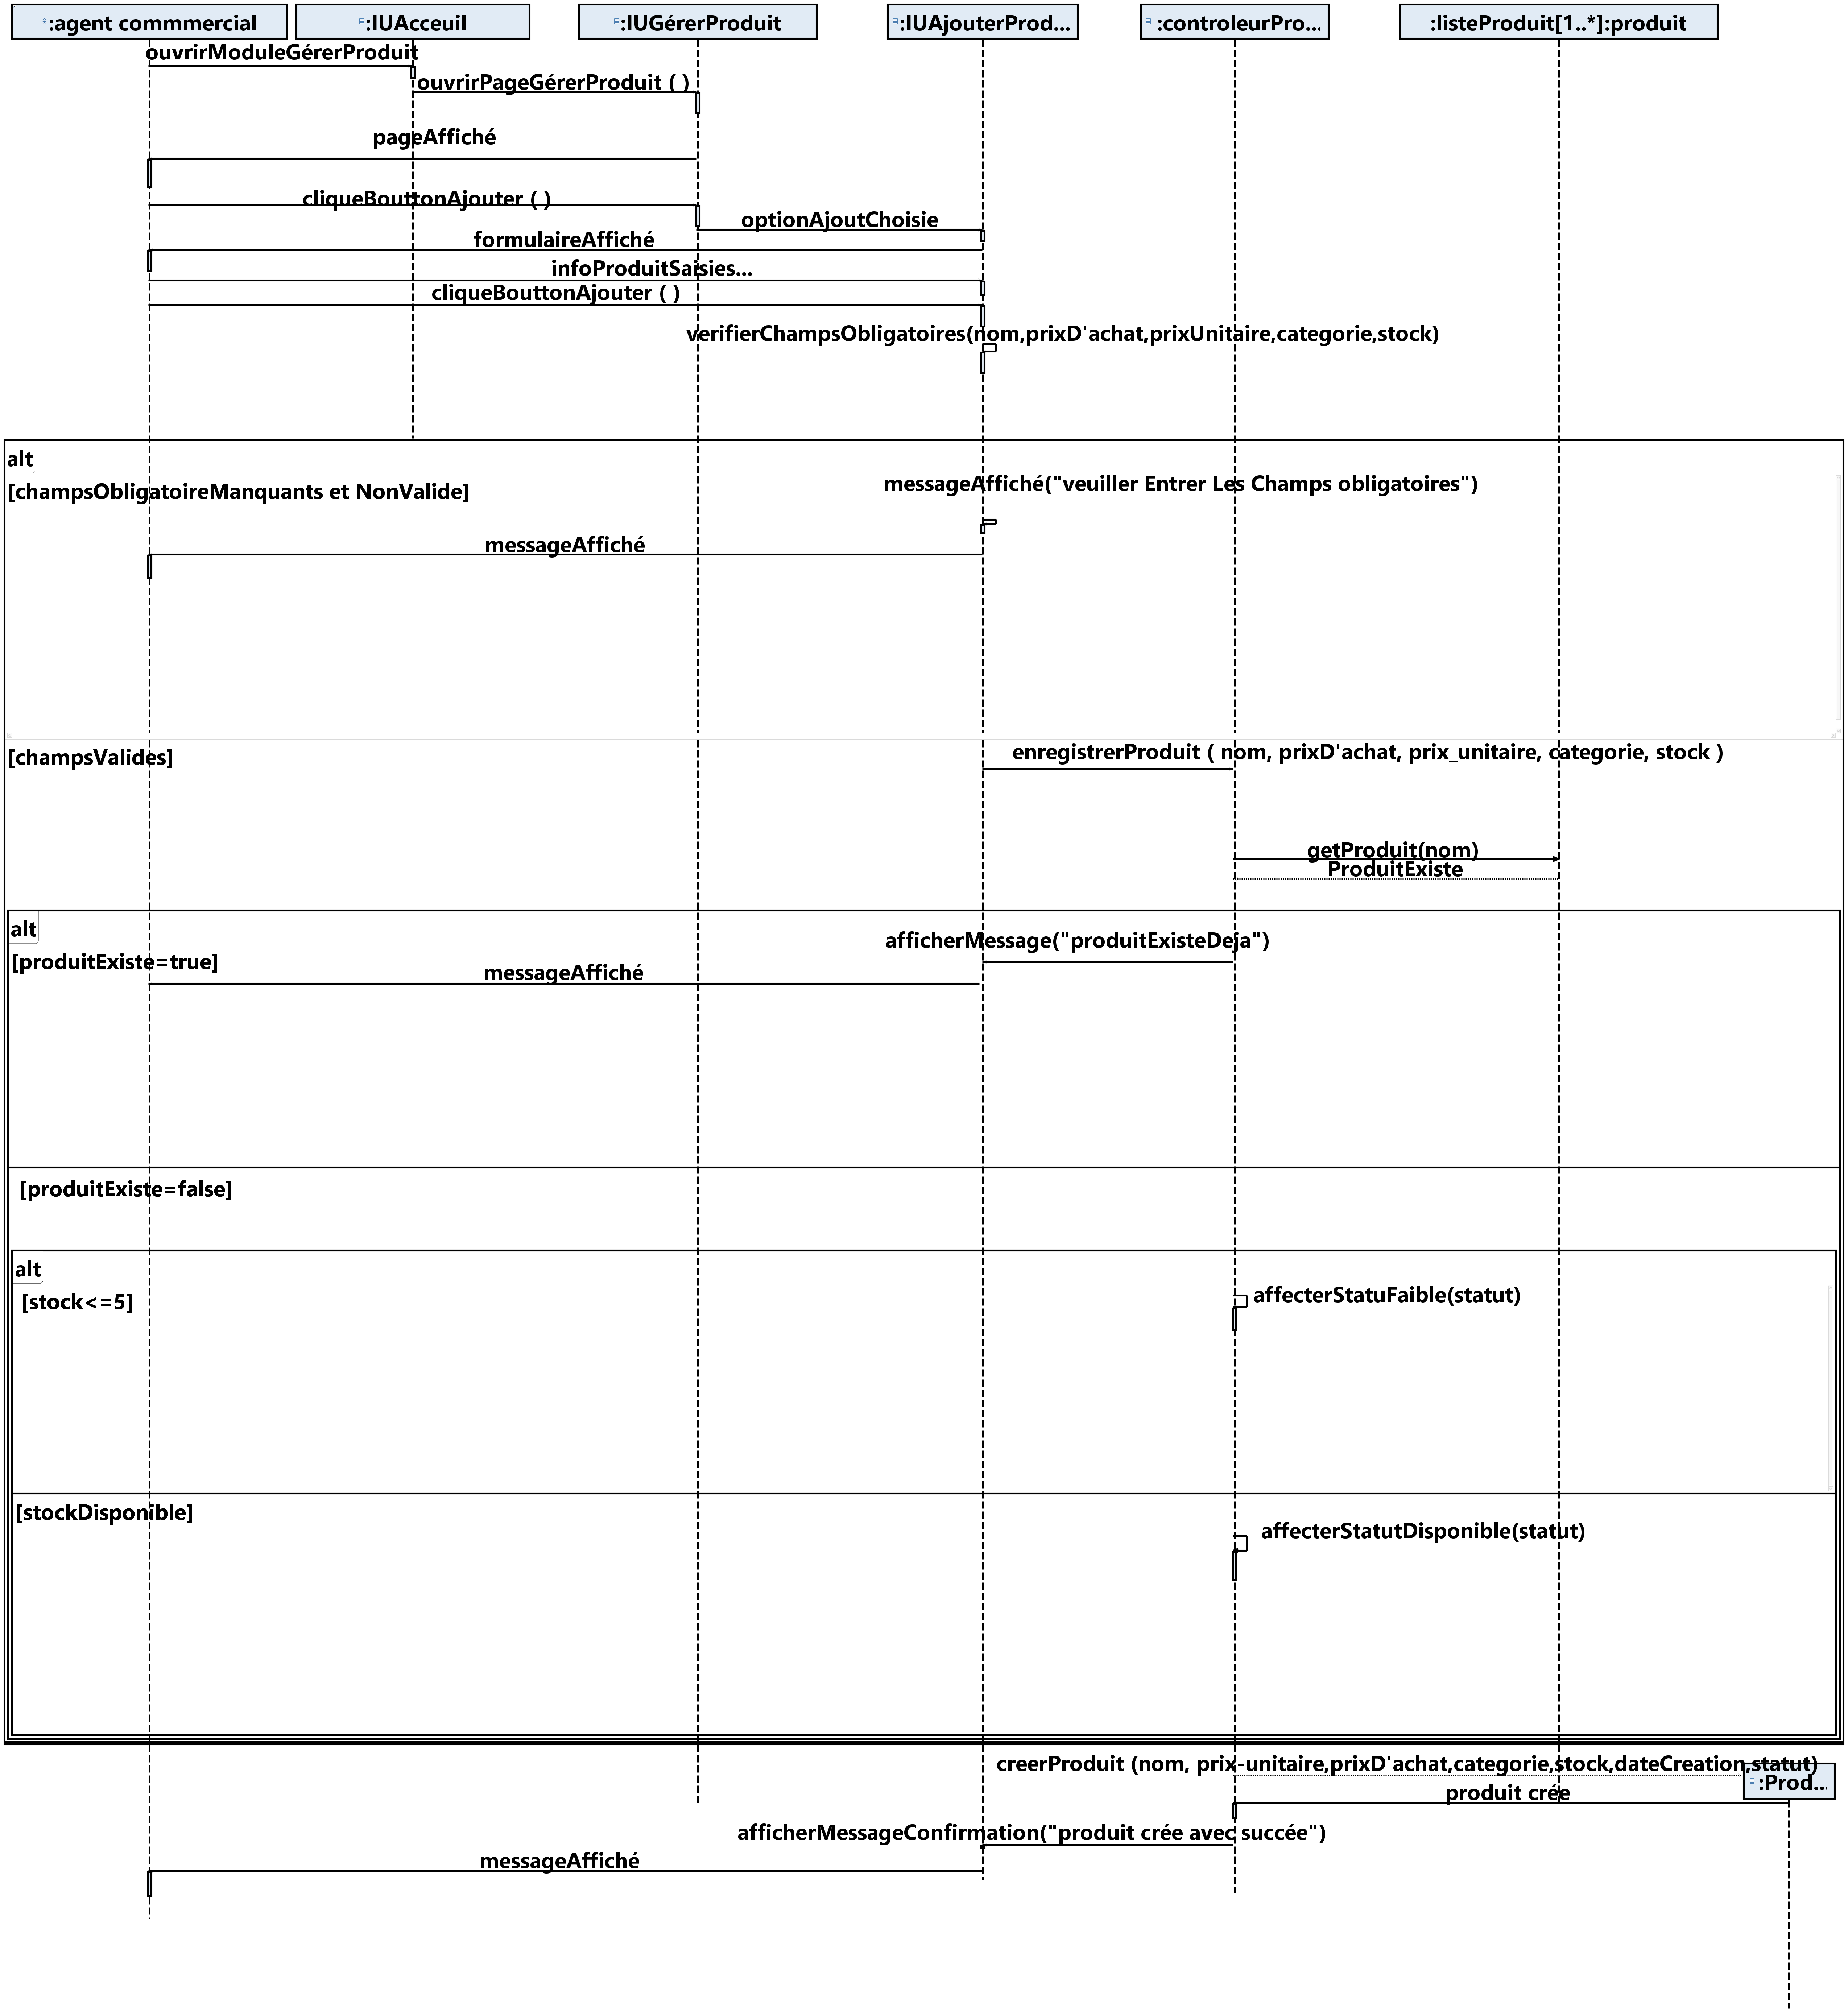
\includegraphics[width=1.15\textwidth, height=0.78\textheight]{images/MC1_DiagrammeSéquenceAjouterProduit_4.png}%
  }
  \caption{Diagramme de séquence pour le cas d'utilisation Ajouter Produit}
  \label{fig:seqAjouterProduit}
\end{figure}

\needspace{0.88\textheight}
\subsection{Diagramme de Séquence du Cas D'utilisation Supprimer Produit}

\begin{figure}[H]
  \centering
  \makebox[\textwidth][c]{%
    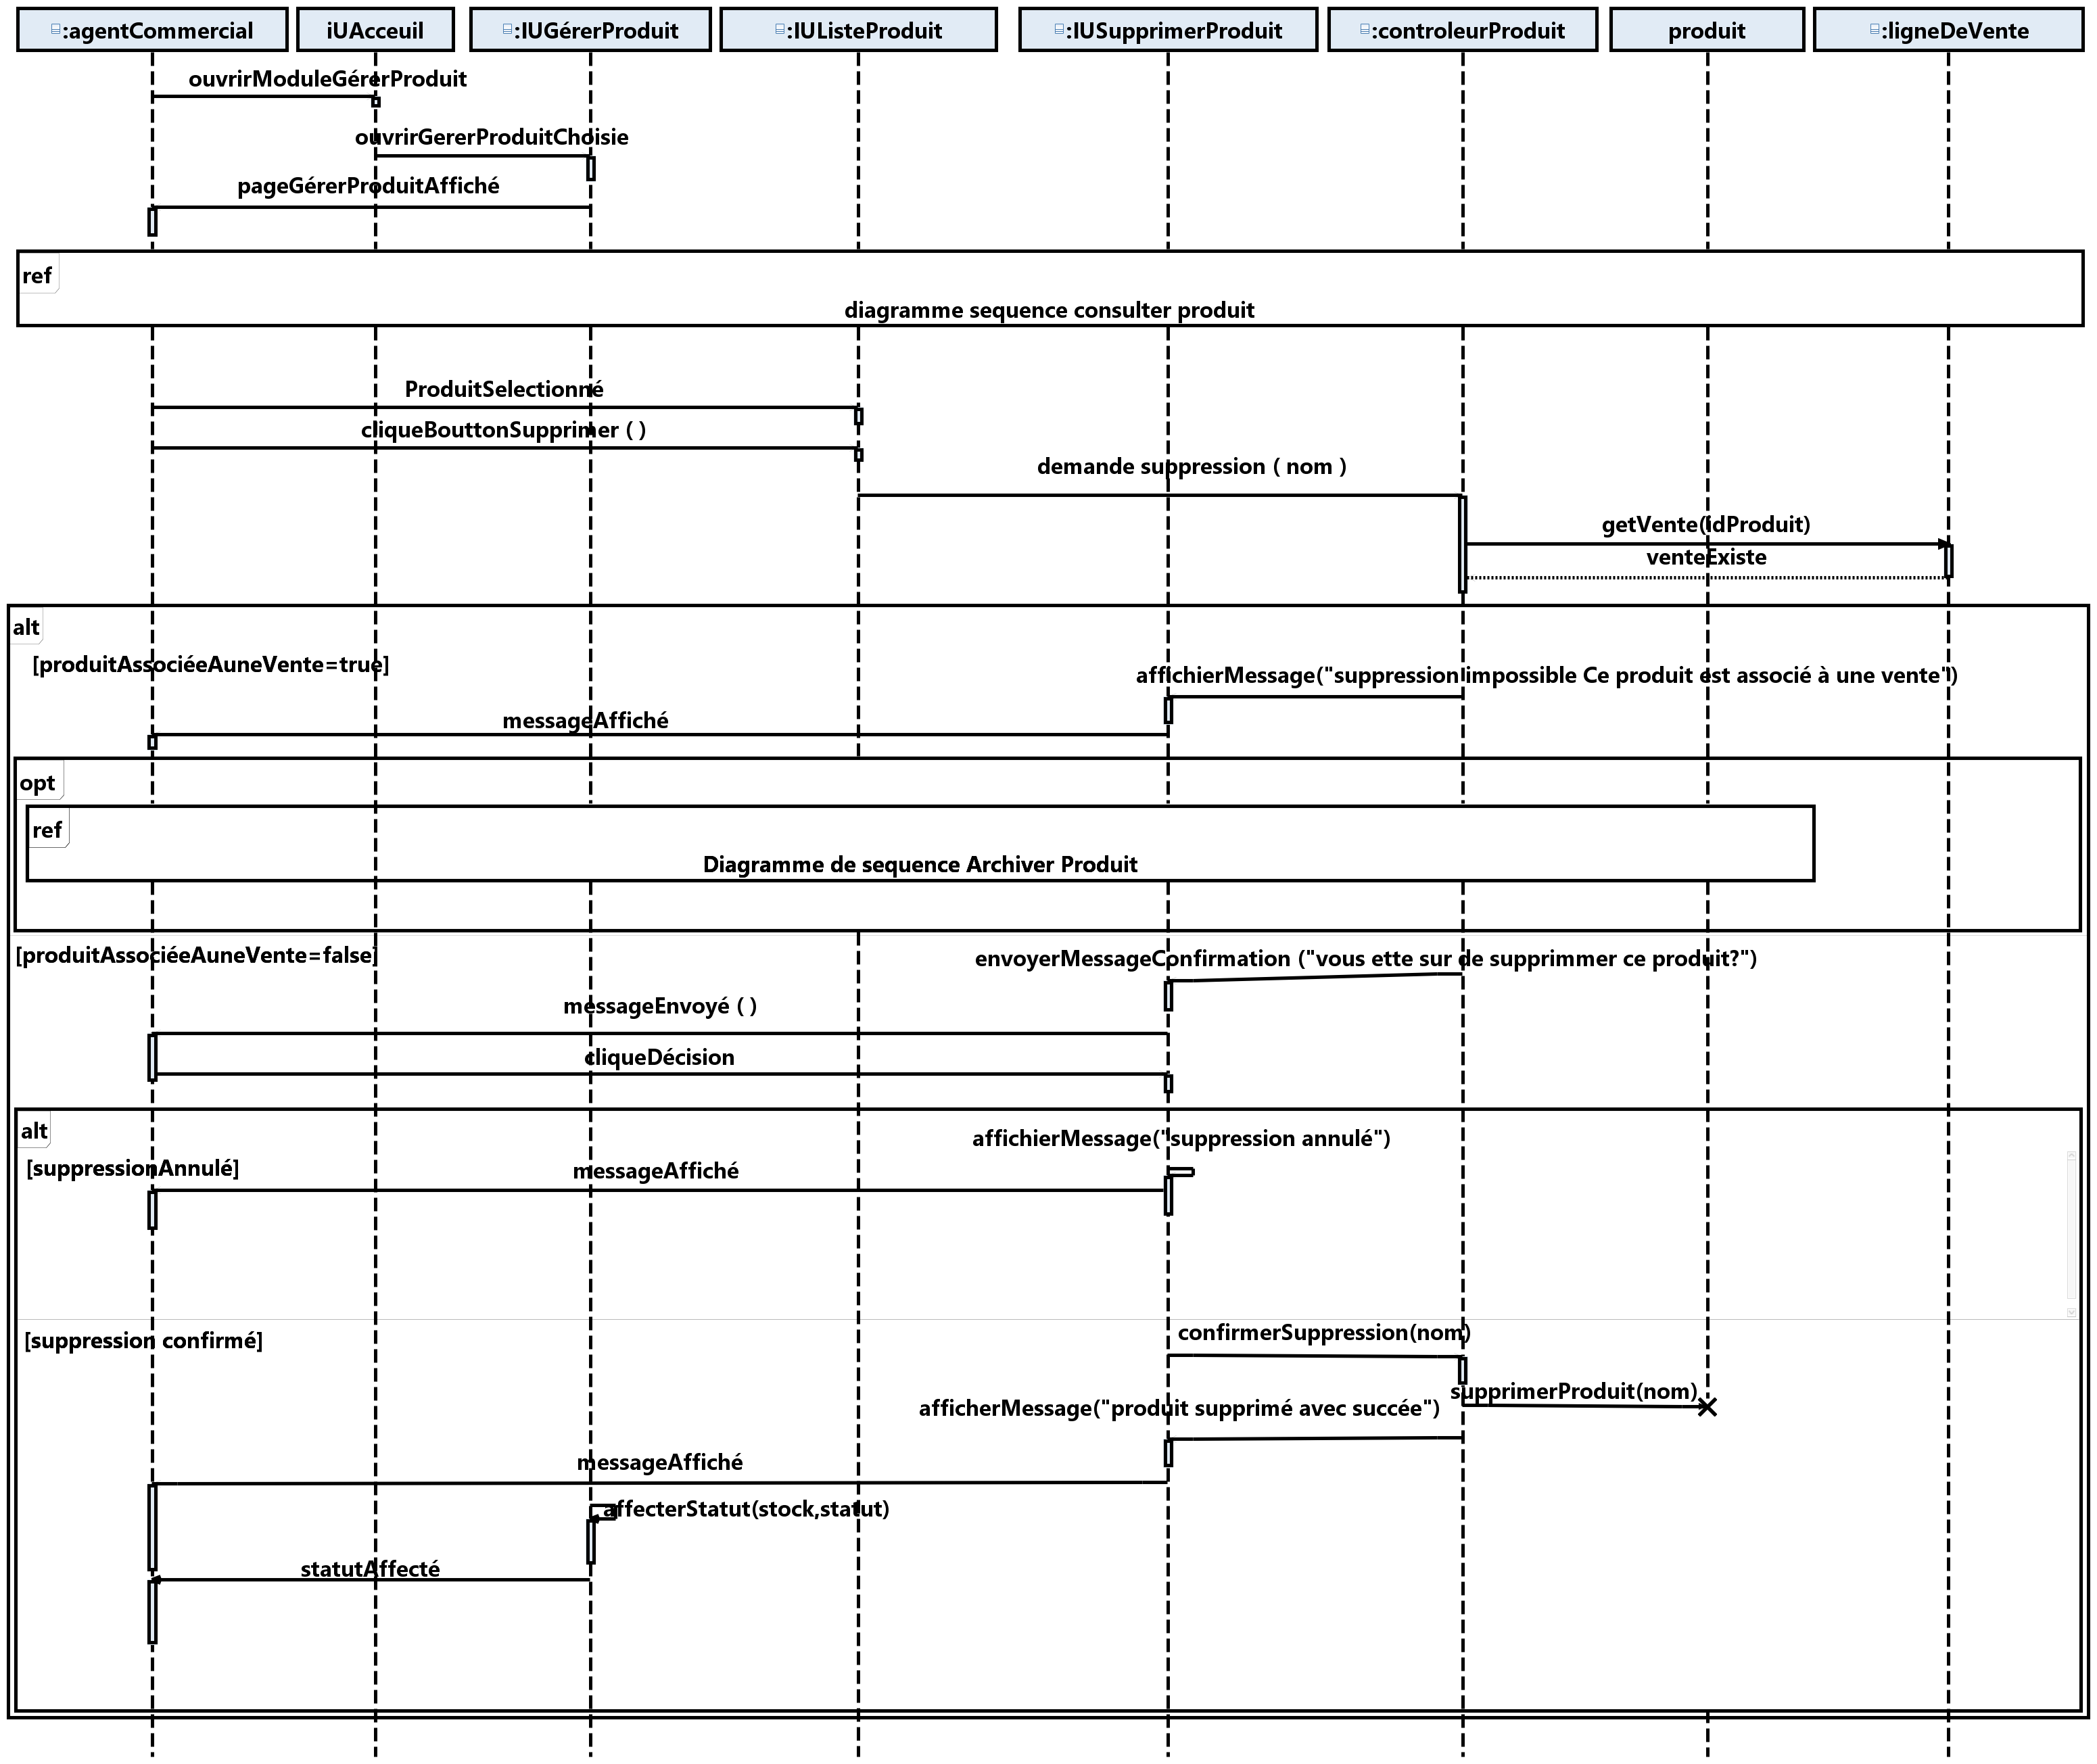
\includegraphics[width=1.15\textwidth, height=0.78\textheight]{images/MC1_DiagrammeSéquenceSupprimerProduit.png}%
  }
  \caption{Diagramme de séquence pour le cas d'utilisation Supprimer Produit}
  \label{fig:seqSupprimerProduit}
\end{figure}

\needspace{0.88\textheight}
\subsection{Diagramme de Séquence du Cas D'utilisation Modifier Produit}

\begin{figure}[H]
  \centering
  \makebox[\textwidth][c]{%
    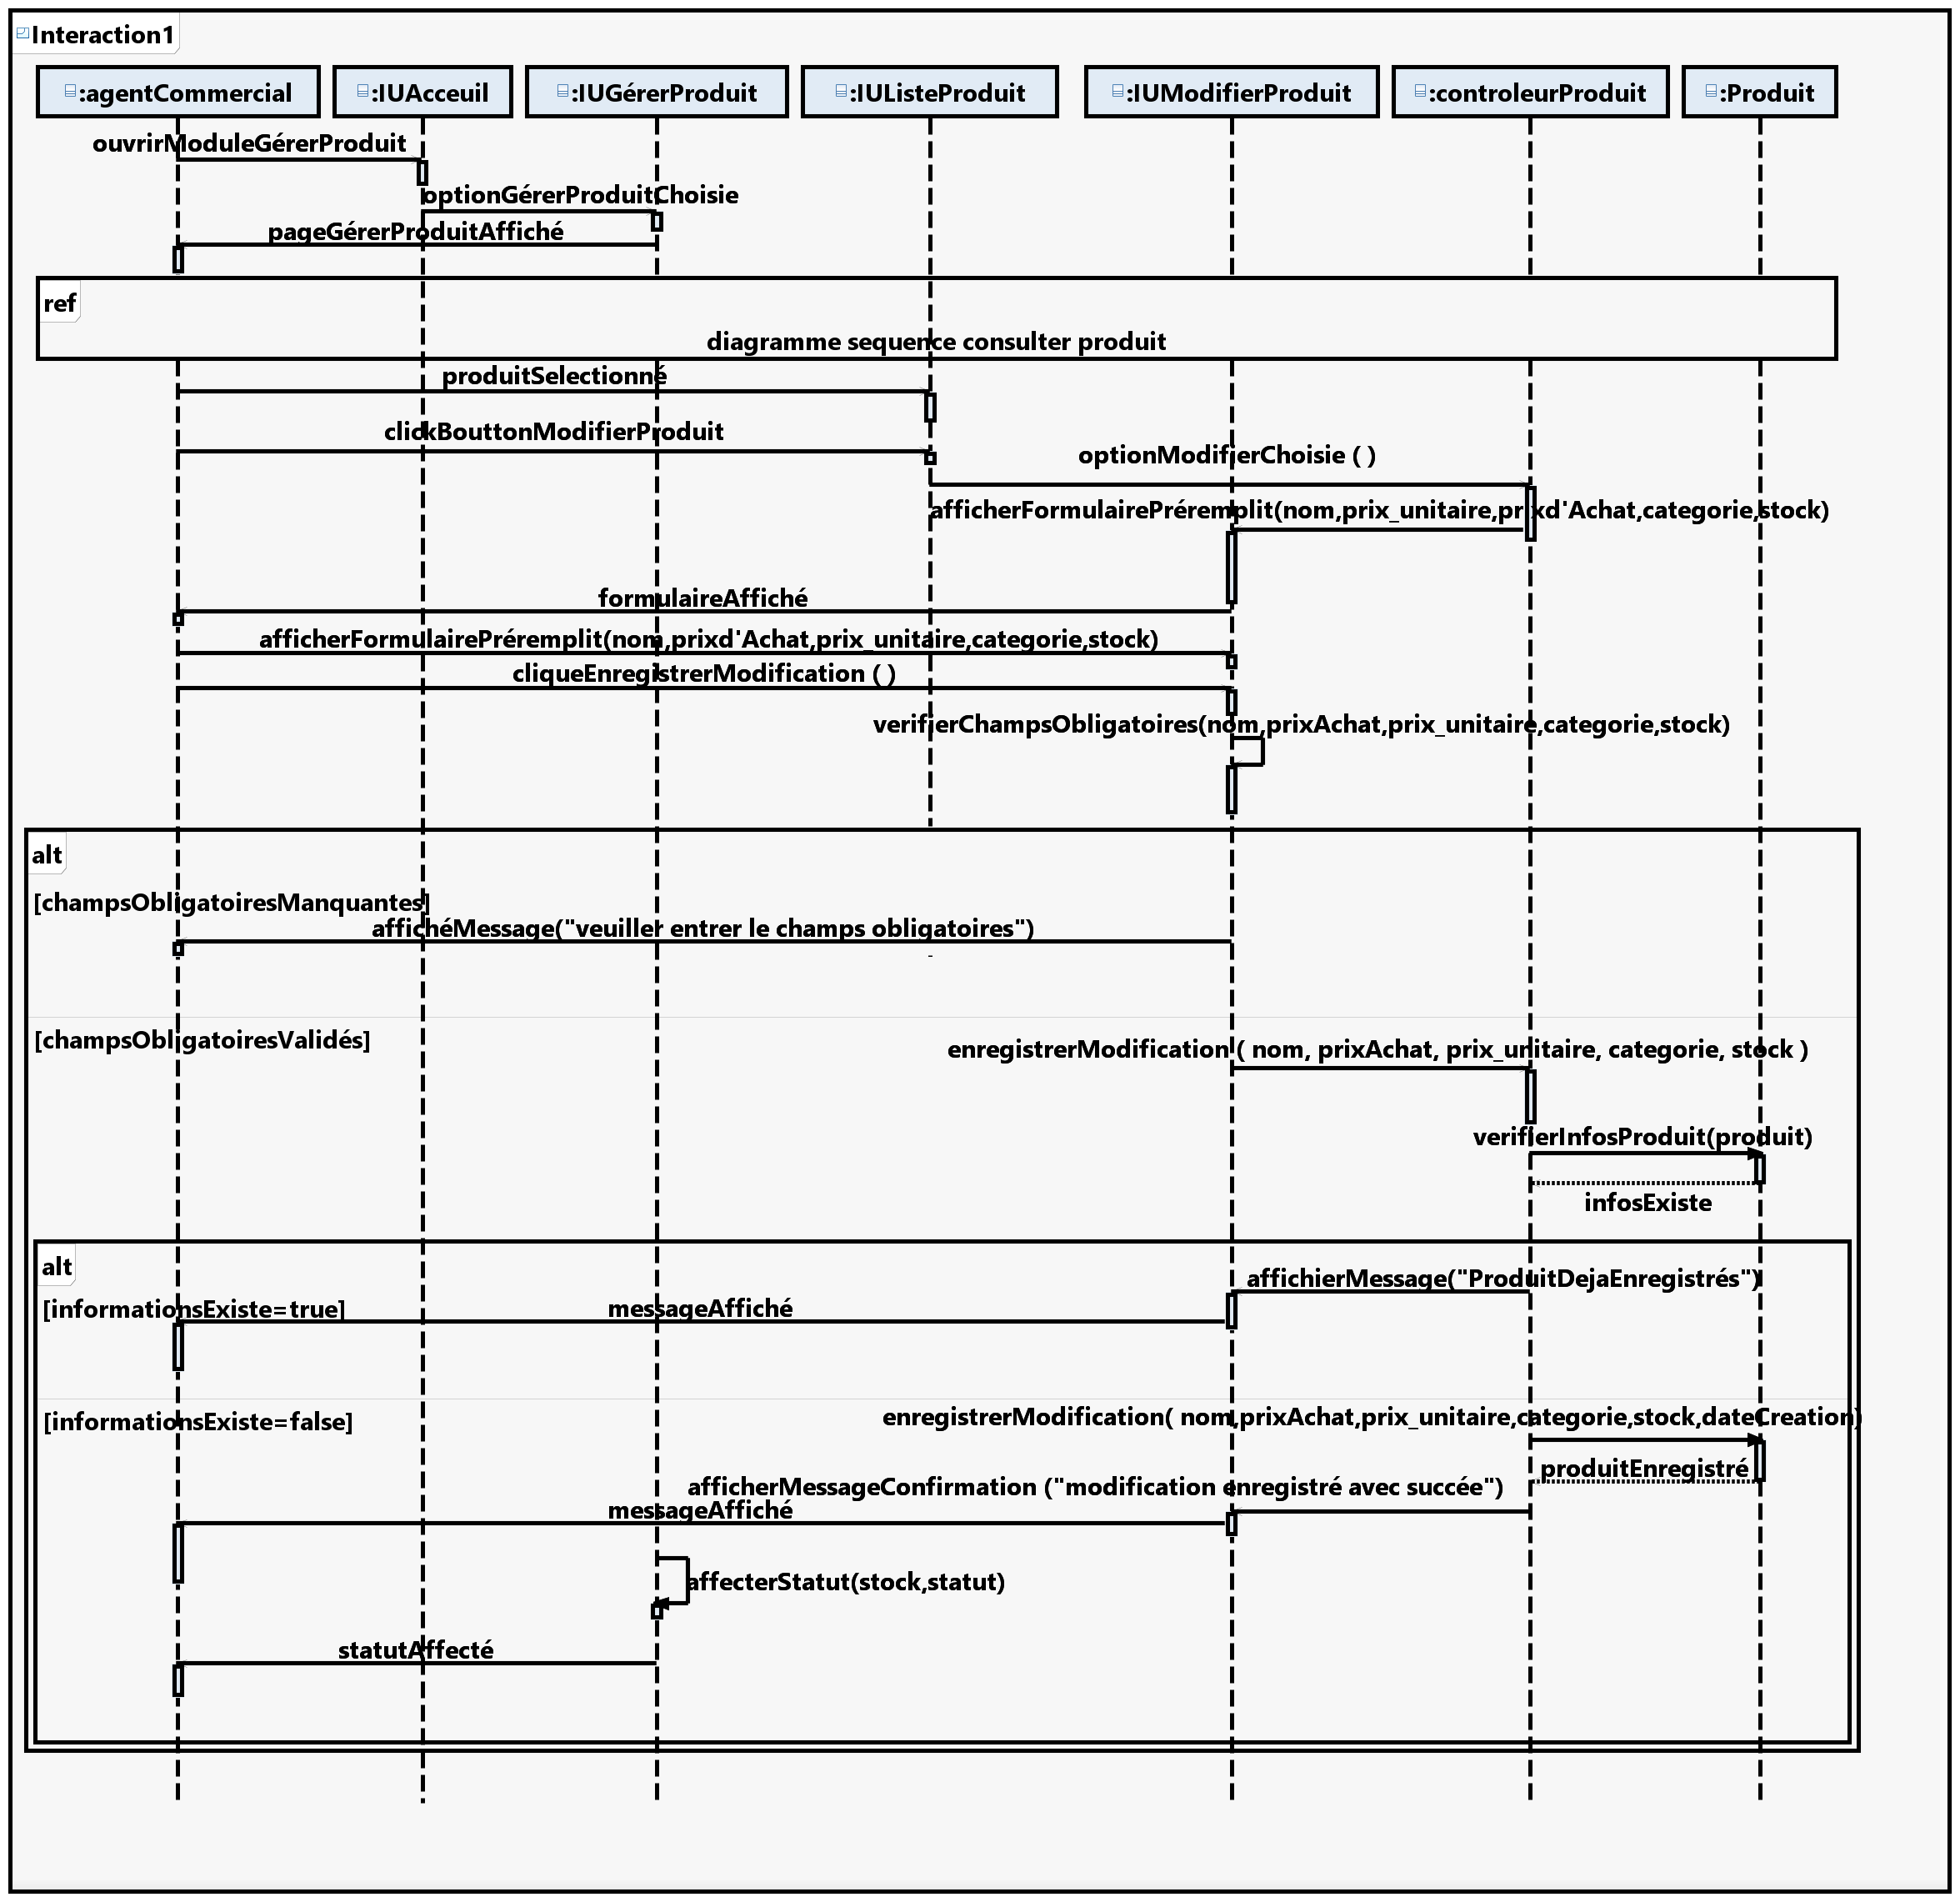
\includegraphics[width=1.15\textwidth, height=0.78\textheight]{images/MC1_DiagrammeSéquenceModifierProduit_2.png}%
  }
  \caption{Diagramme de séquence pour le cas d'utilisation Modifier Produit}
  \label{fig:seqModifierProduit}
\end{figure}

\needspace{0.88\textheight}
\subsection{Diagramme de Séquence du Cas D'utilisation Consulter Produit}

\begin{figure}[H]
  \centering
  \makebox[\textwidth][c]{%
    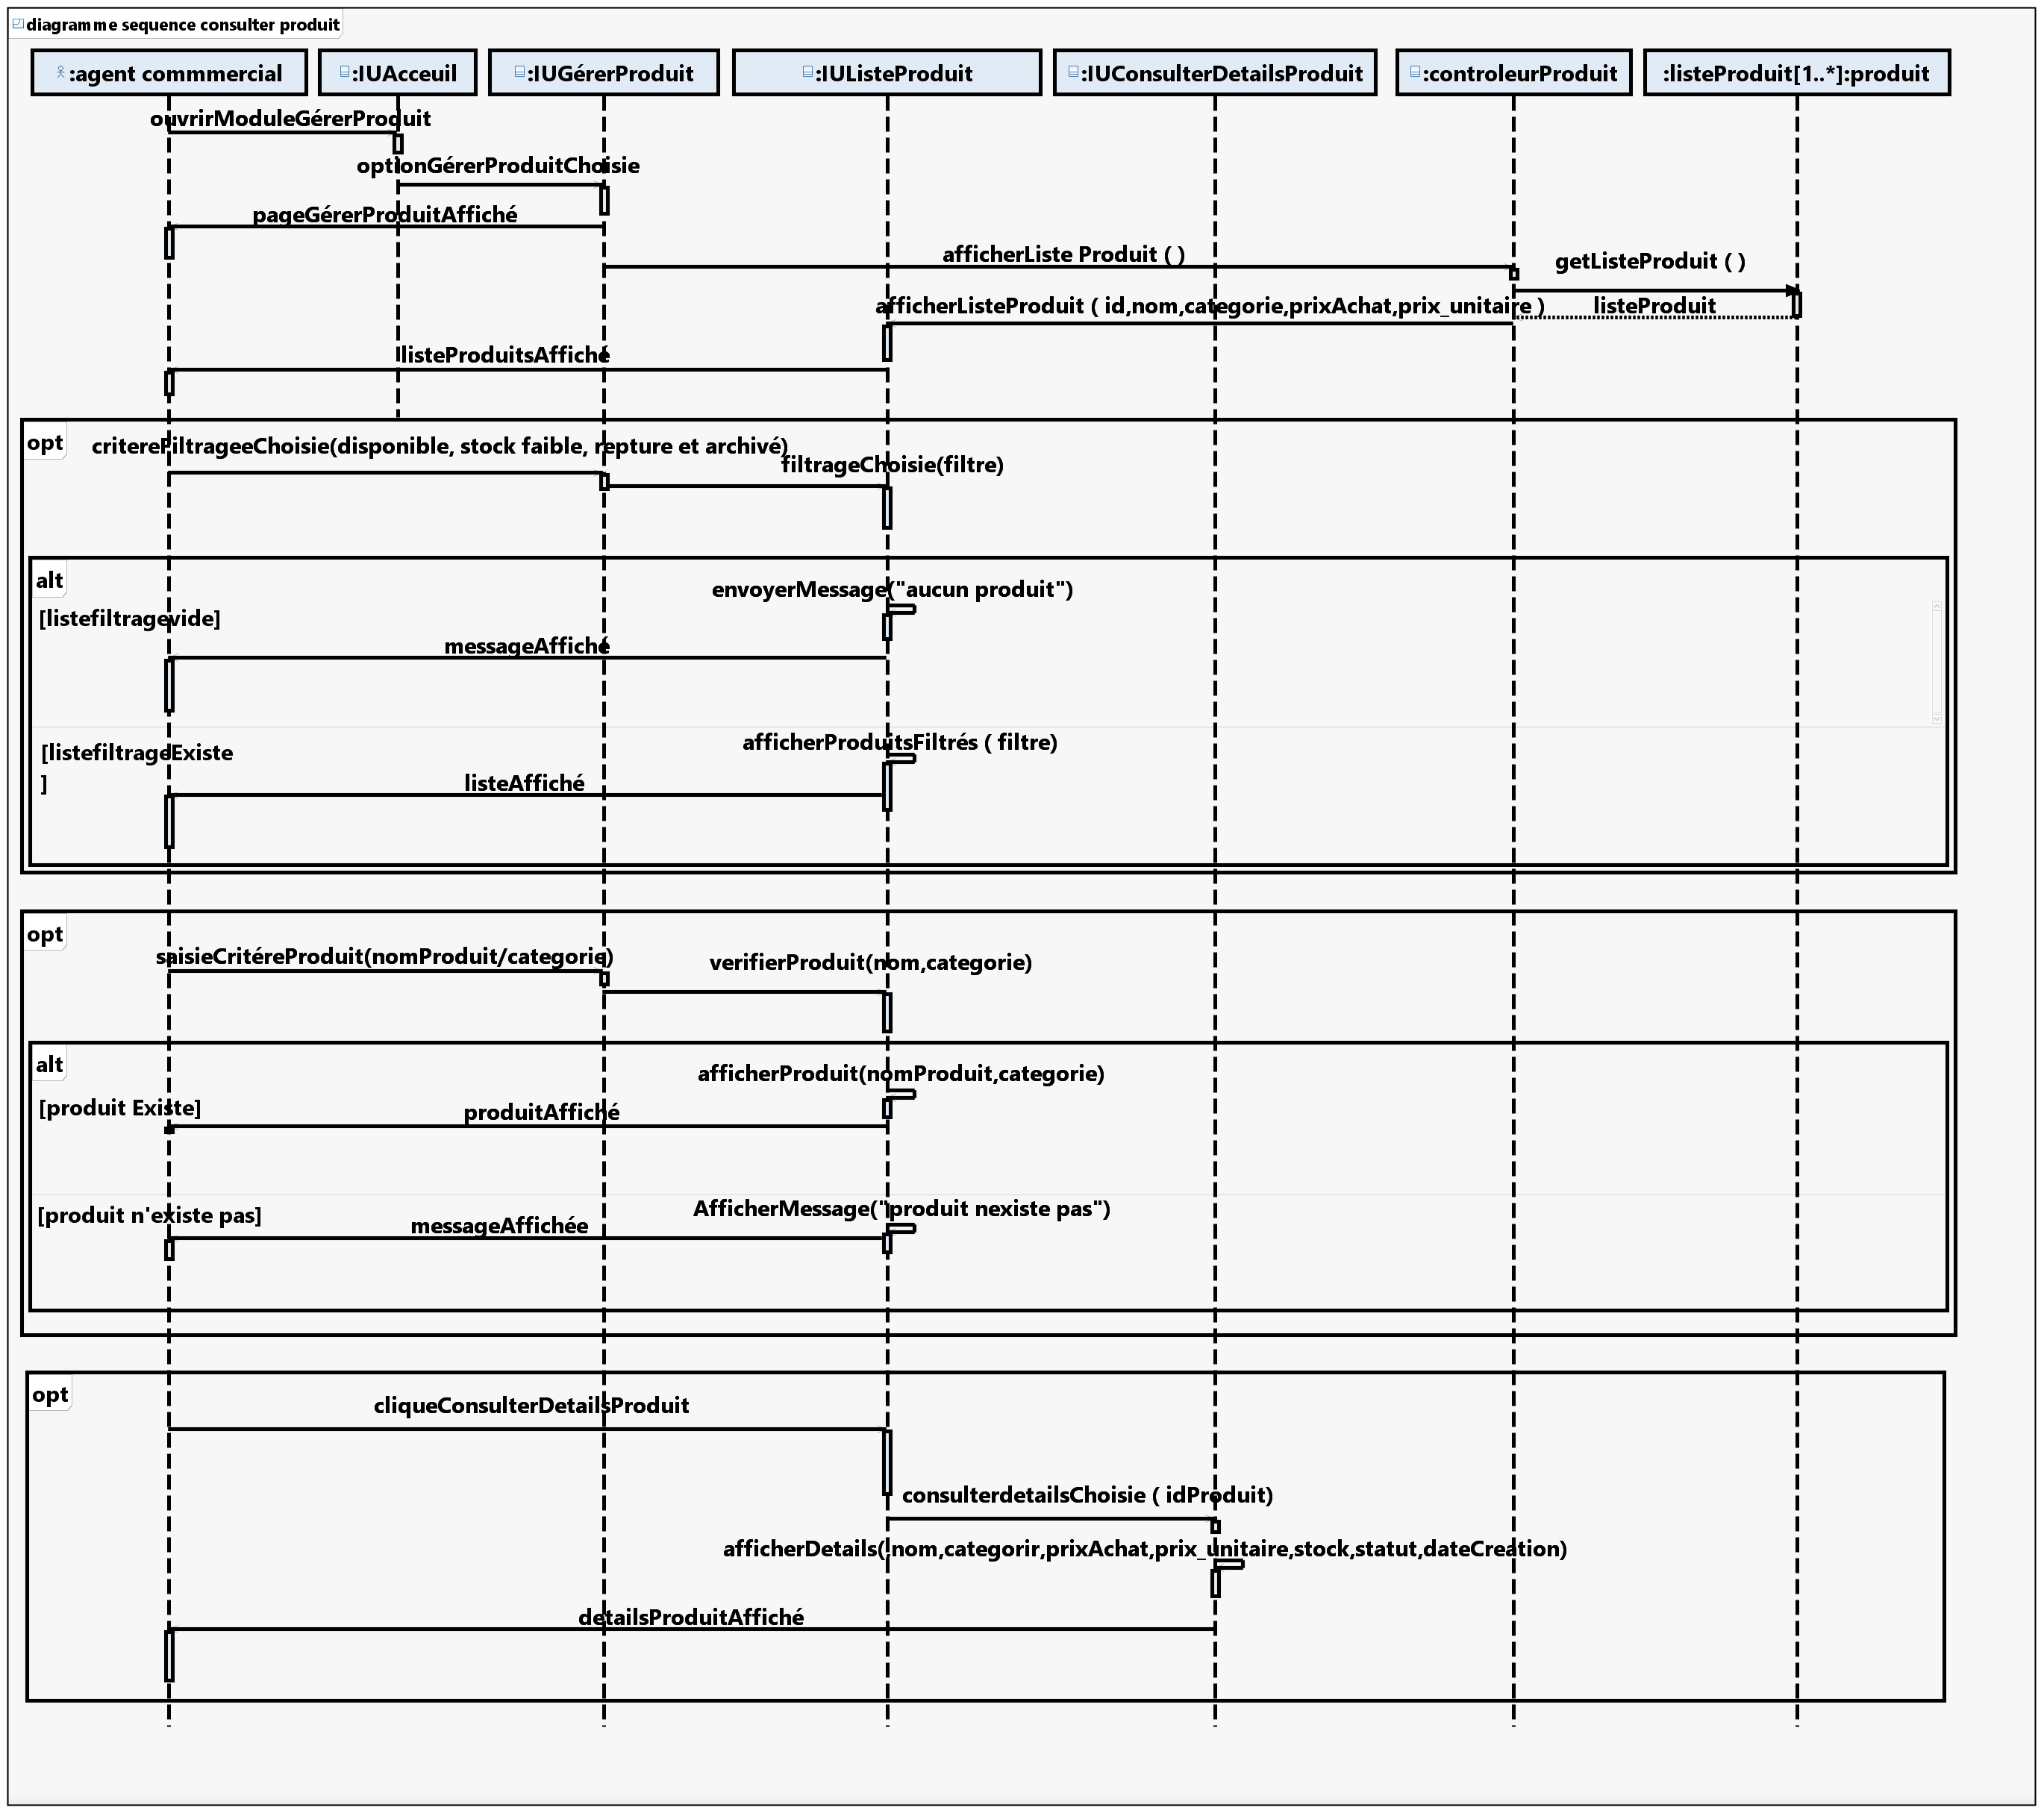
\includegraphics[width=1.15\textwidth, height=0.78\textheight]{images/MC_DiagrammeSéquenceConsulterProduit.png}%
  }
  \caption{Diagramme de séquence pour le cas d'utilisation Consulter Produit}
  \label{fig:seqConsulterProduit}
\end{figure}

\needspace{0.88\textheight}
\subsection{Diagramme de Séquence du Cas D'utilisation Archiver Produit}
Il est à noter que le CEO peut également effectuer les mêmes opérations de gestion des produits que l'agent commercial.
\begin{figure}[H]
  \centering
  \makebox[\textwidth][c]{%
    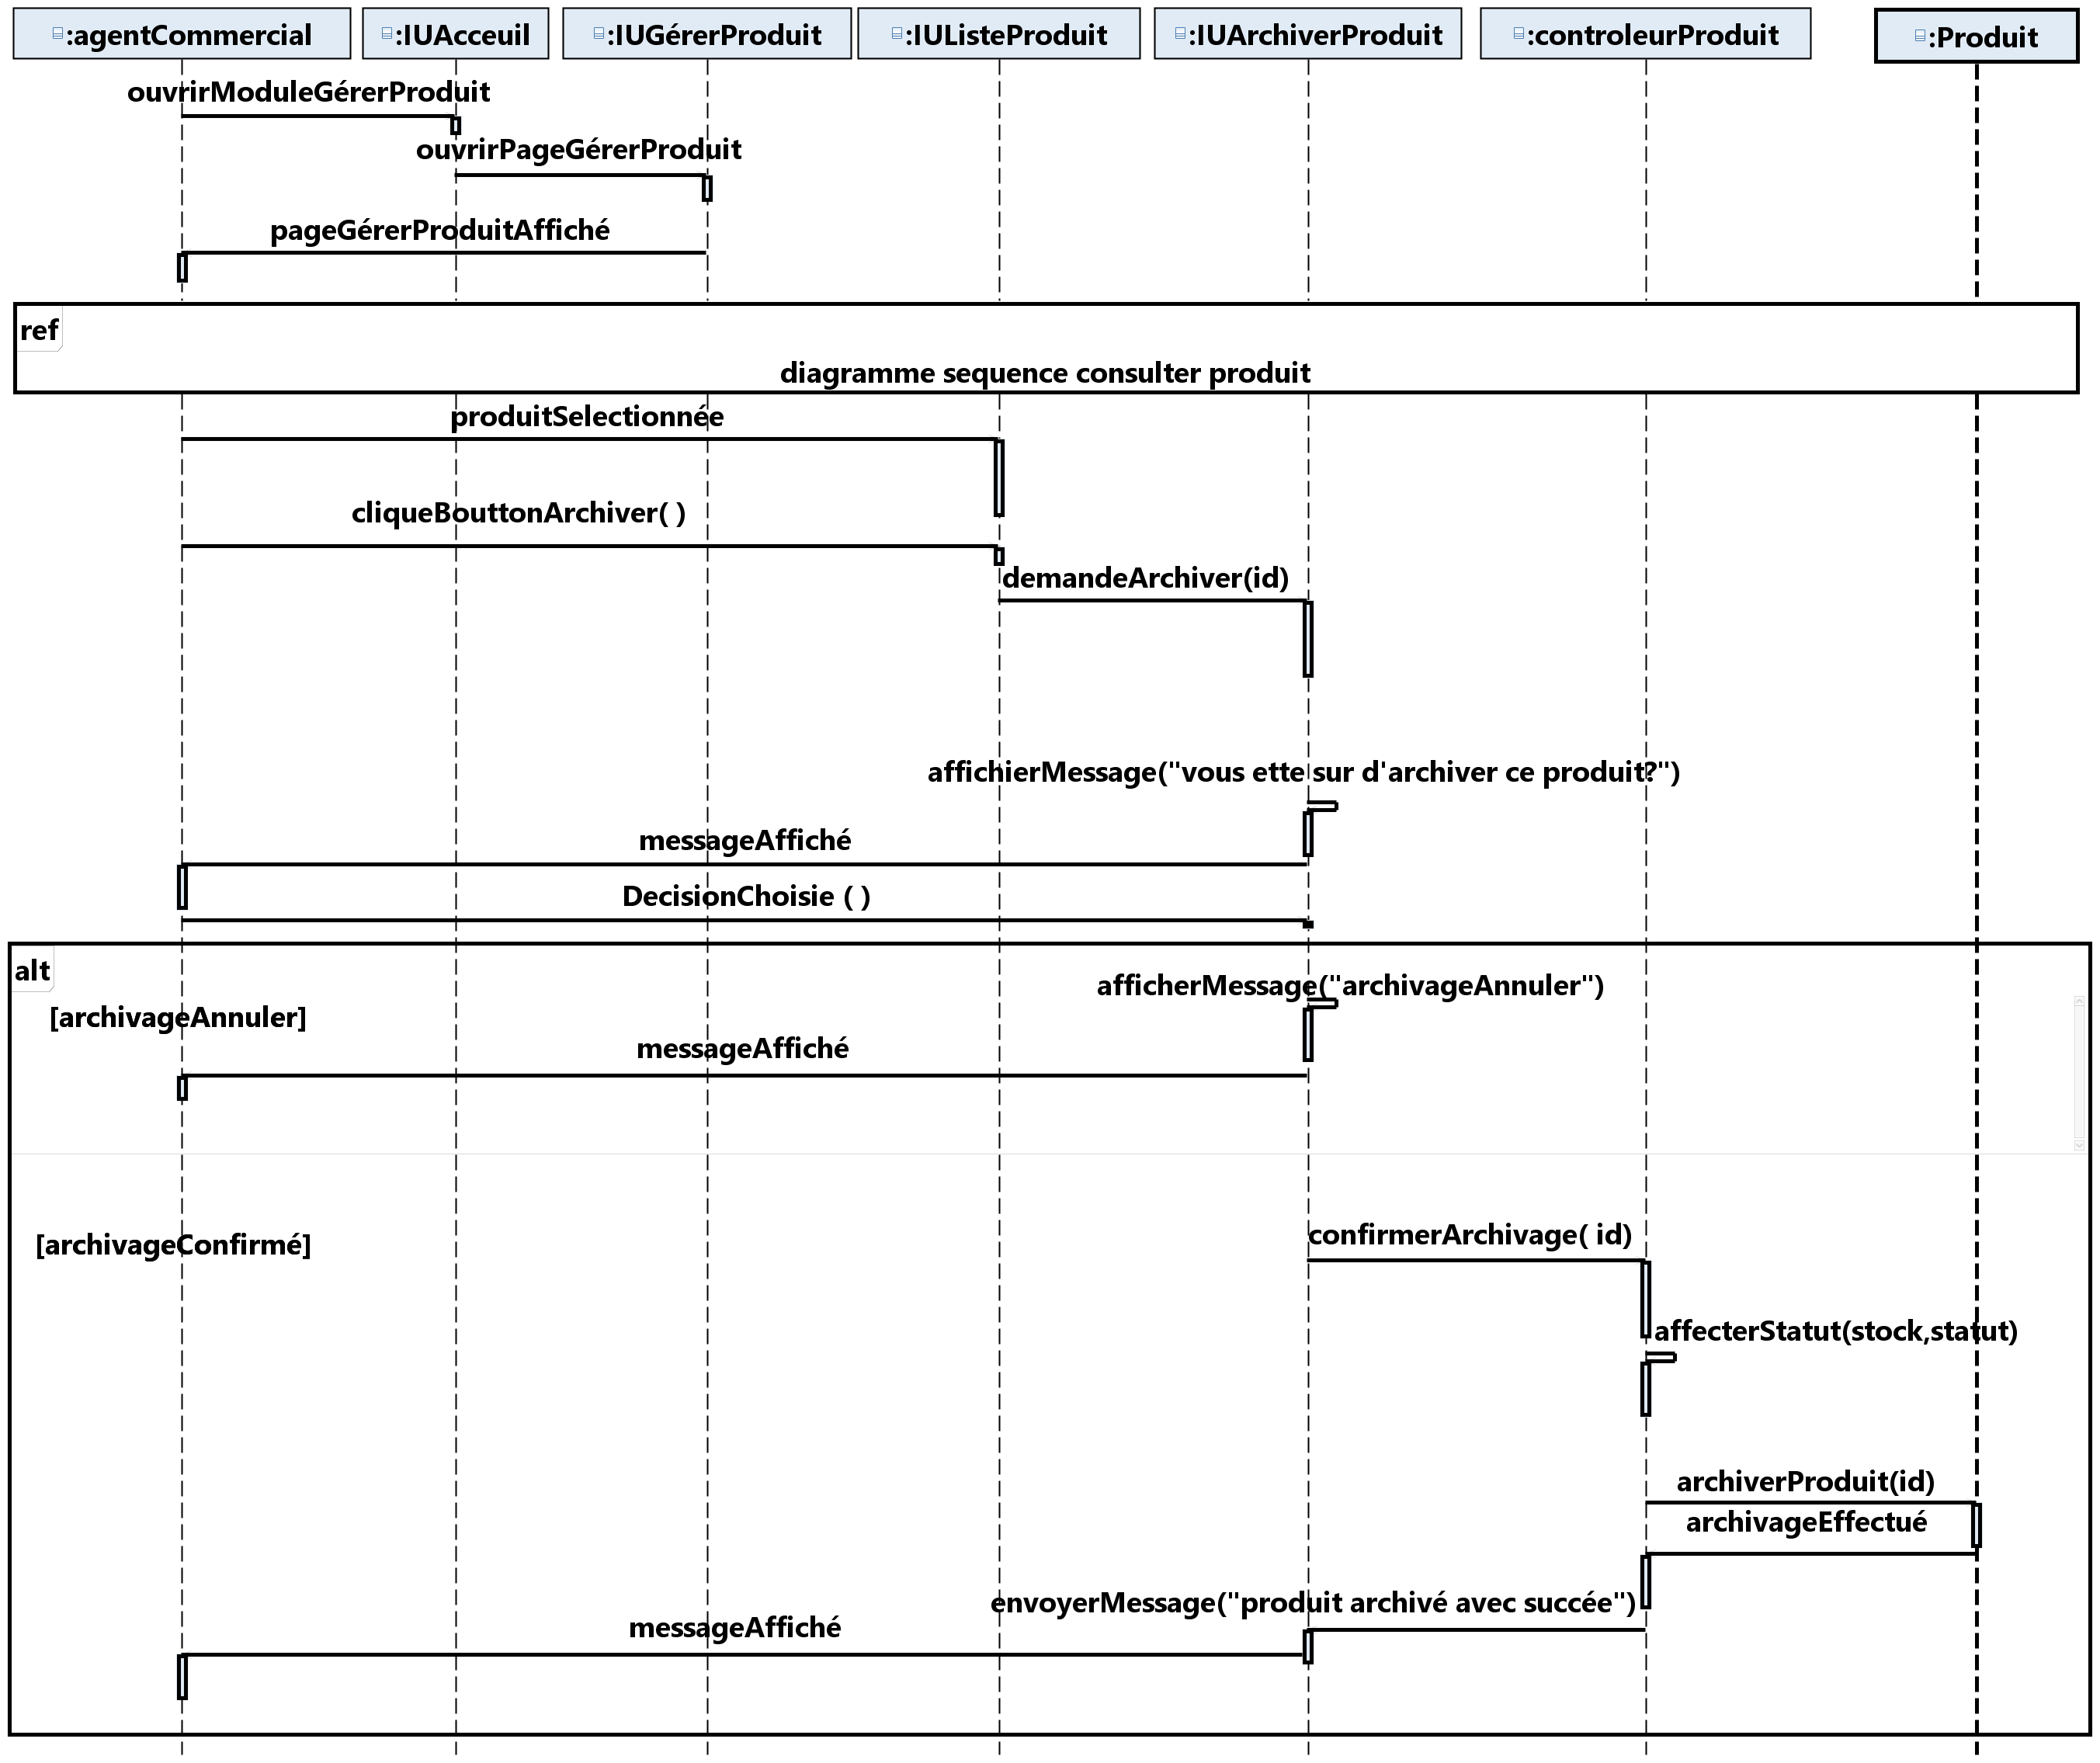
\includegraphics[width=1.15\textwidth, height=0.78\textheight]{images/MC1_DiagrammeSéquenceArchiverProduit_1.png}%
  }
  \caption{Diagramme de séquence pour le cas d'utilisation Archiver Produit}
  \label{fig:seqArchiverProduit} 
\end{figure}
\newpage

\needspace{0.88\textheight}
\subsection{Diagramme de Classe du Cas D'utilisation Gérer Produits}

\begin{figure}[H]
  \centering
  \makebox[\textwidth][c]{%
    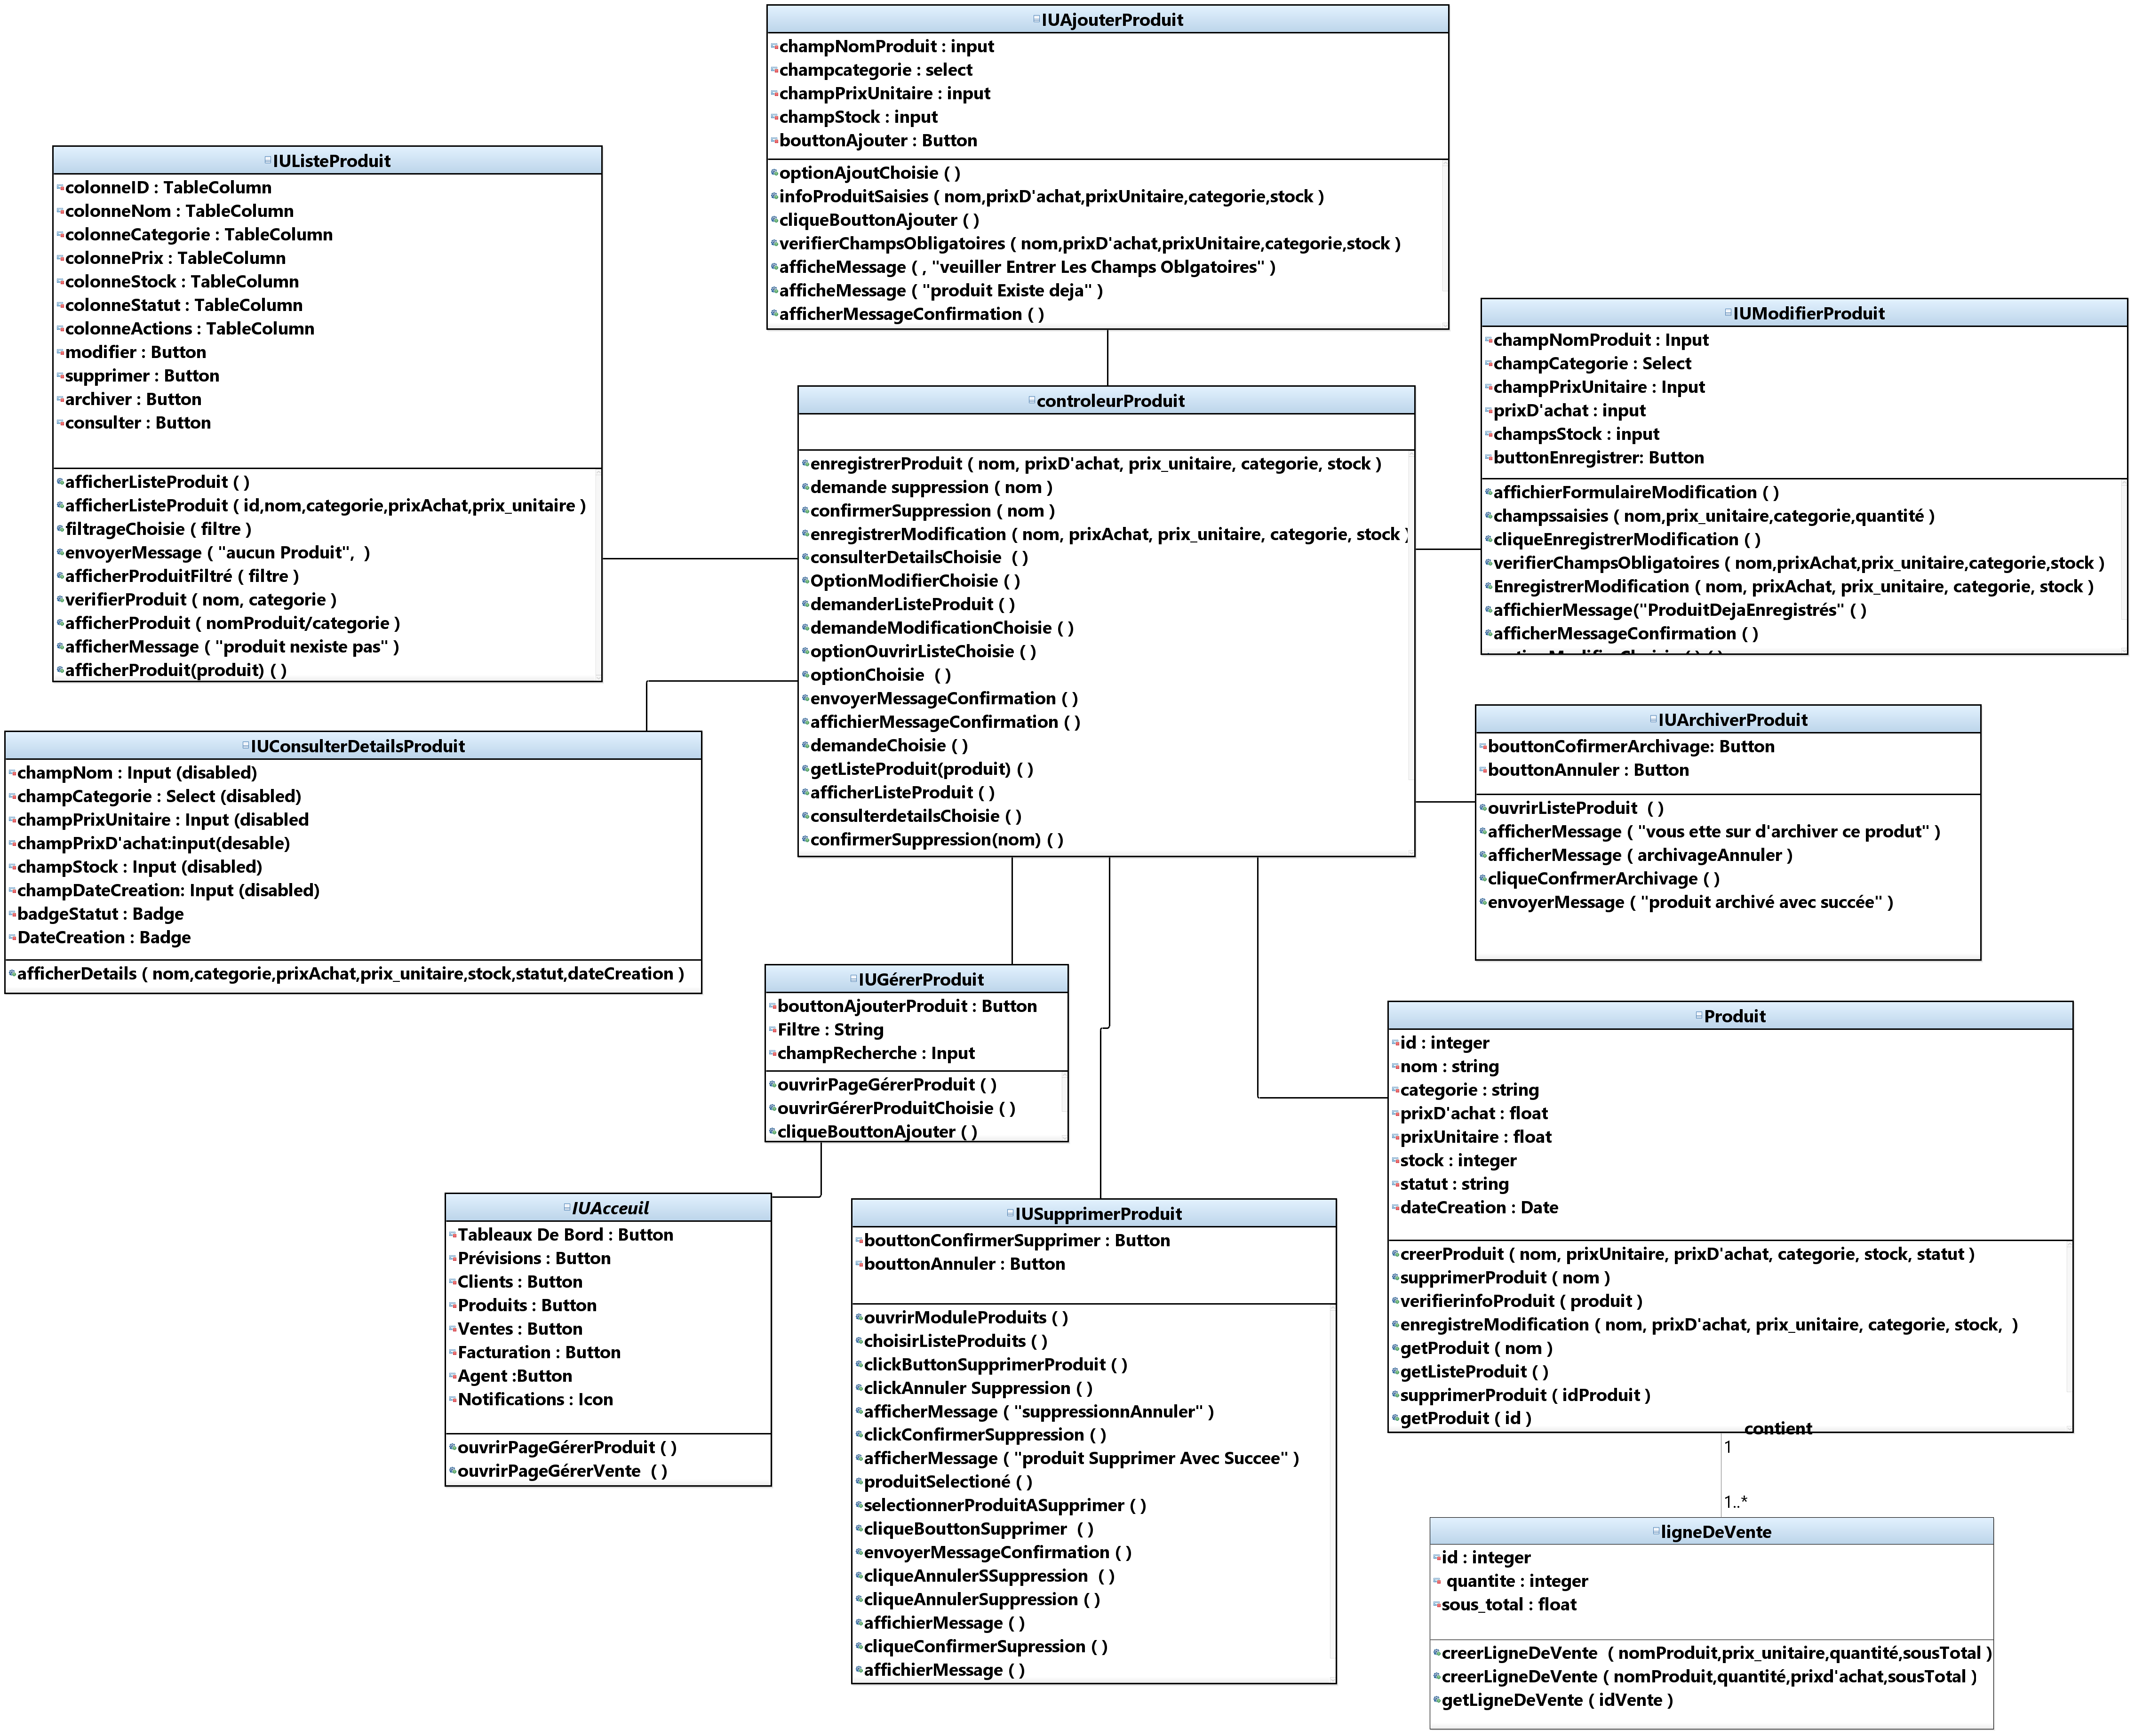
\includegraphics[width=1.15\textwidth, height=0.78\textheight]{images/MC1_DiagrammeClasseGérerProduit.png}%
  }
  \caption{Diagramme de classe pour le cas d'utilisation Gérer Produits}
  \label{fig:classeProduits}
\end{figure}
\newpage

\section{Conception du Cas D'utilisation Gérer Clients}

\needspace{0.88\textheight}
\subsection{Traçabilité MCU/MC pour le Cas D'utilisation Gérer Clients}

\begin{figure}[H]
  \centering
  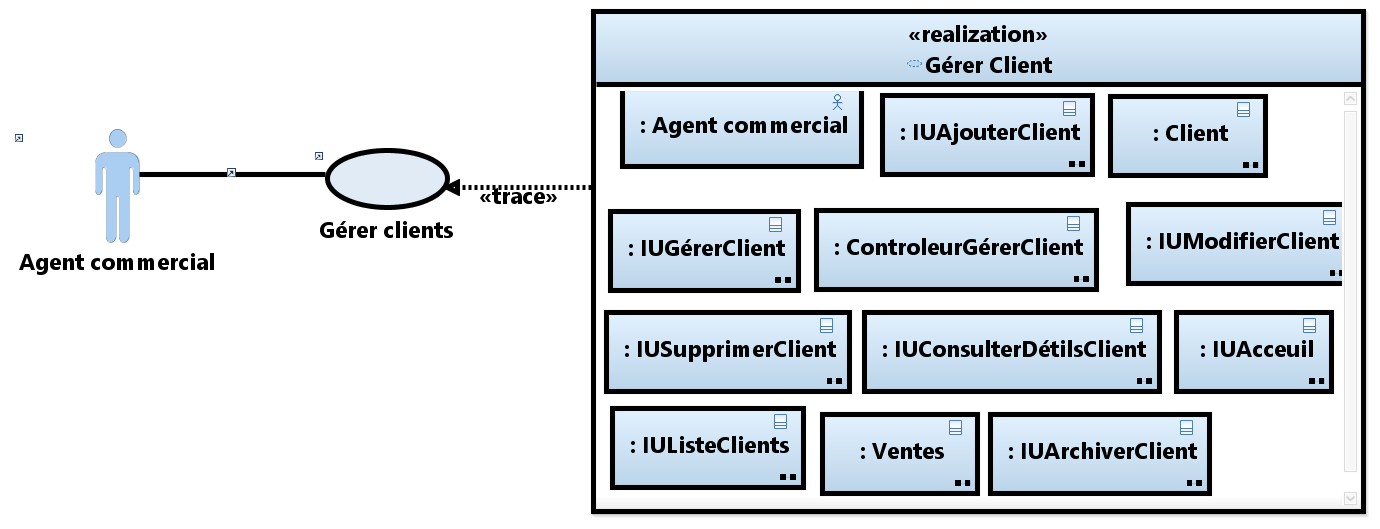
\includegraphics[width=\textwidth]{images/MC_tracabiliteMCUMCGererClient.png}
  \caption{Traçabilité MCU/MC pour le cas d'utilisation Gérer Clients}
\end{figure}

Cette traçabilité montre quels sont les objets instances de classe participant à la réalisation du cas d'utilisation Gérer Clients.

L'acteur et Les classes impliquées dans ce diagramme sont les suivantes :

\begin{itemize}[leftmargin=2em, topsep=4pt, itemsep=4pt]
  \item \textbf{Agent Commercial :} l'acteur qui initie les opérations de gestion des clients
  \item \textbf{IUGérerClient :} l'interface principale qui affiche les options de gestion des clients
  \item \textbf{IUAccueil :} l'interface principale depuis laquelle l'agent accède à la page de gestion des clients
  \item \textbf{IUAjouterClient :} l'interface qui permet à l'agent commercial d'ajouter un nouveau client en définissant son prénom, nom, email, téléphone, ville et adresse
  \item \textbf{IUModifierClient :} l'interface qui permet à l'agent commercial de modifier les informations d'un client existant
  \item \textbf{IUSupprimerClient :} l'interface qui permet à l'agent commercial de confirmer la suppression d'un client du système
  \item \textbf{IUArchiverClient :} l'interface qui permet à l'agent commercial de confirmer l'archivage d'un client
  \item \textbf{IUConsulterDetailsClient :} l'interface qui permet à l'agent commercial de consulter les informations détaillées d'un client sélectionné
  \newpage
  \item \textbf{IUListeClient :} l'interface qui affiche la liste des clients avec les options de recherche et de filtrage
  \item \textbf{ControleurGérerClient :} permet de gérer les flux de contrôle entre l'interface et l'entité client
  \item \textbf{Client :} l'entité du système qui contient les  données et les traitements métier relative aux clients
  \item \textbf{Vente :} l'entité du système qui contient les  données et les traitements métier aux ventes associées à chaque client
\end{itemize}

Il est à noter que le CEO peut également effectuer les mêmes opérations de gestion des clients que l'agent commercial.

\needspace{0.88\textheight}
\subsection{Diagramme de Séquence du Cas D'utilisation Ajouter Client}

\begin{figure}[H]
  \centering
  \makebox[\textwidth][c]{%
    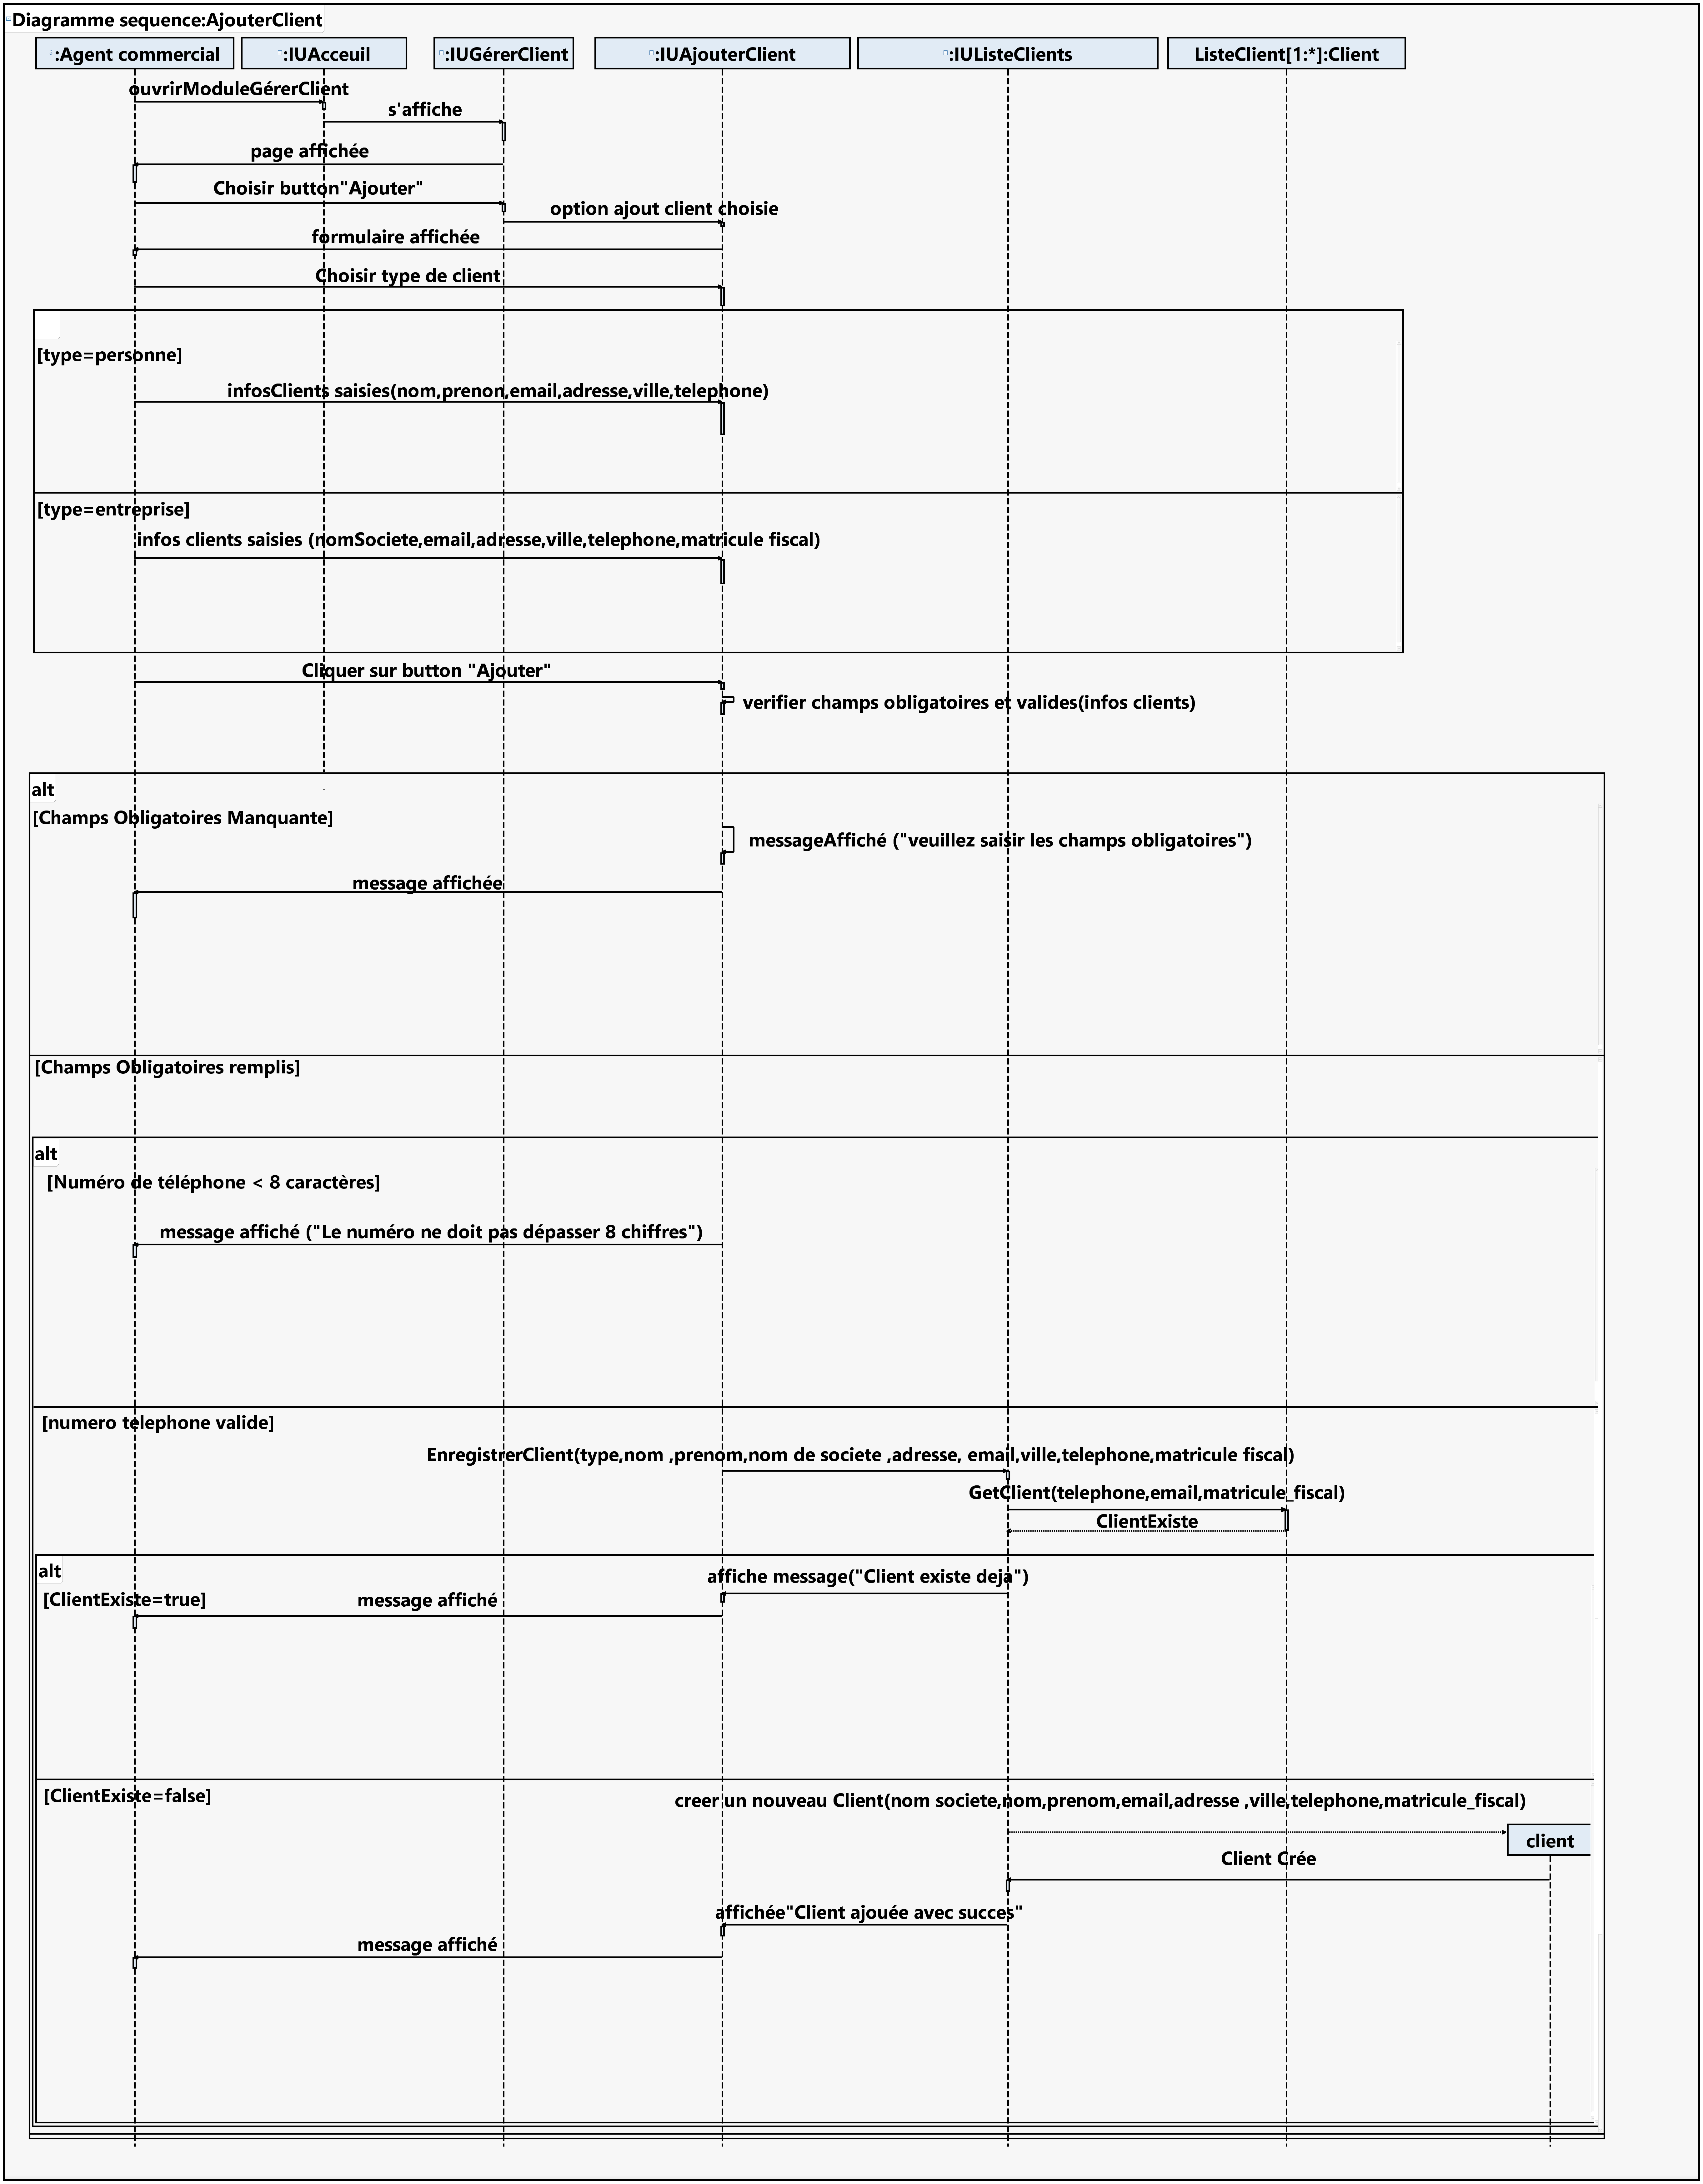
\includegraphics[width=1.15\textwidth, height=0.78\textheight]{images/MC_diagseqAjouterClient_1.png}%
  }
  \caption{Diagramme de séquence pour le cas d'utilisation Ajouter Client}
  \label{fig:seqAjouterClient}
\end{figure}

\needspace{0.88\textheight}
\subsection{Diagramme de Séquence du Cas D'utilisation Modifier Client}

\begin{figure}[H]
  \centering
  \makebox[\textwidth][c]{%
    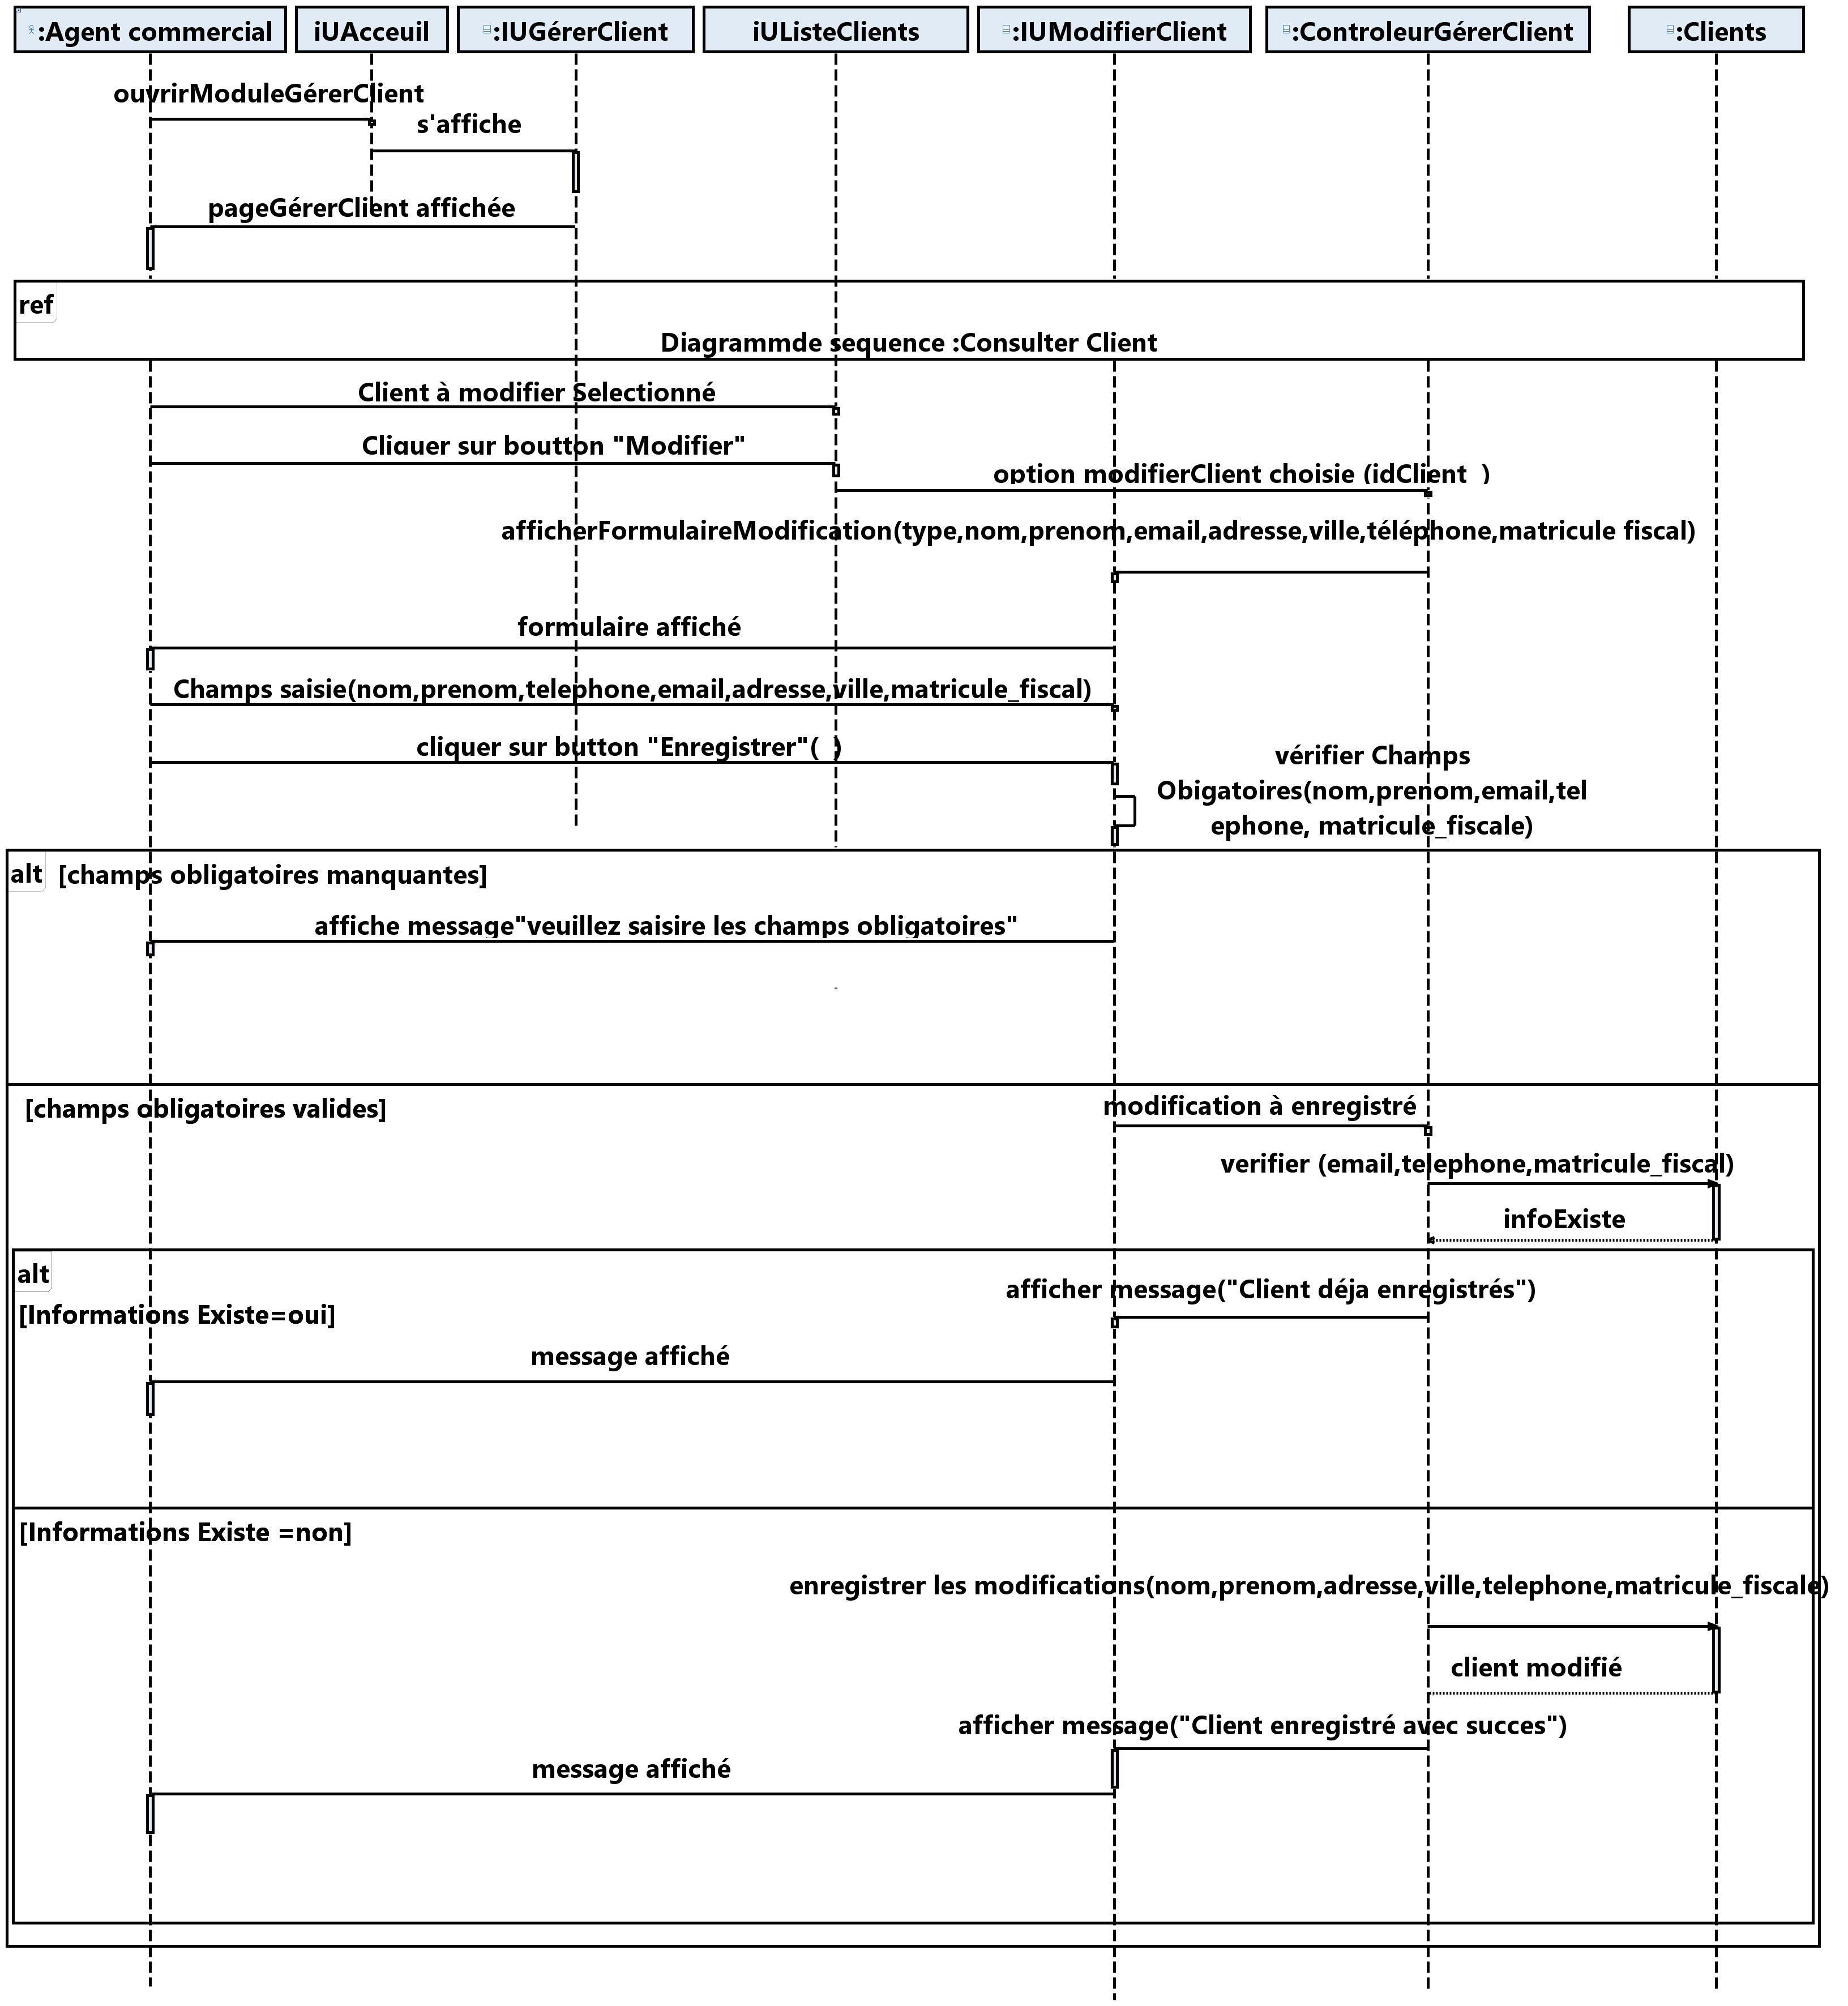
\includegraphics[width=1.15\textwidth, height=0.78\textheight]{images/MC_DiagrammeSéquenceModifierClient_1.png}%
  }
  \caption{Diagramme de séquence pour le cas d'utilisation Modifier Client}
  \label{fig:seqModifierClient}
\end{figure}

\needspace{0.88\textheight}
\subsection{Diagramme de Séquence du Cas D'utilisation Supprimer Client}

\begin{figure}[H]
  \centering
  \makebox[\textwidth][c]{%
    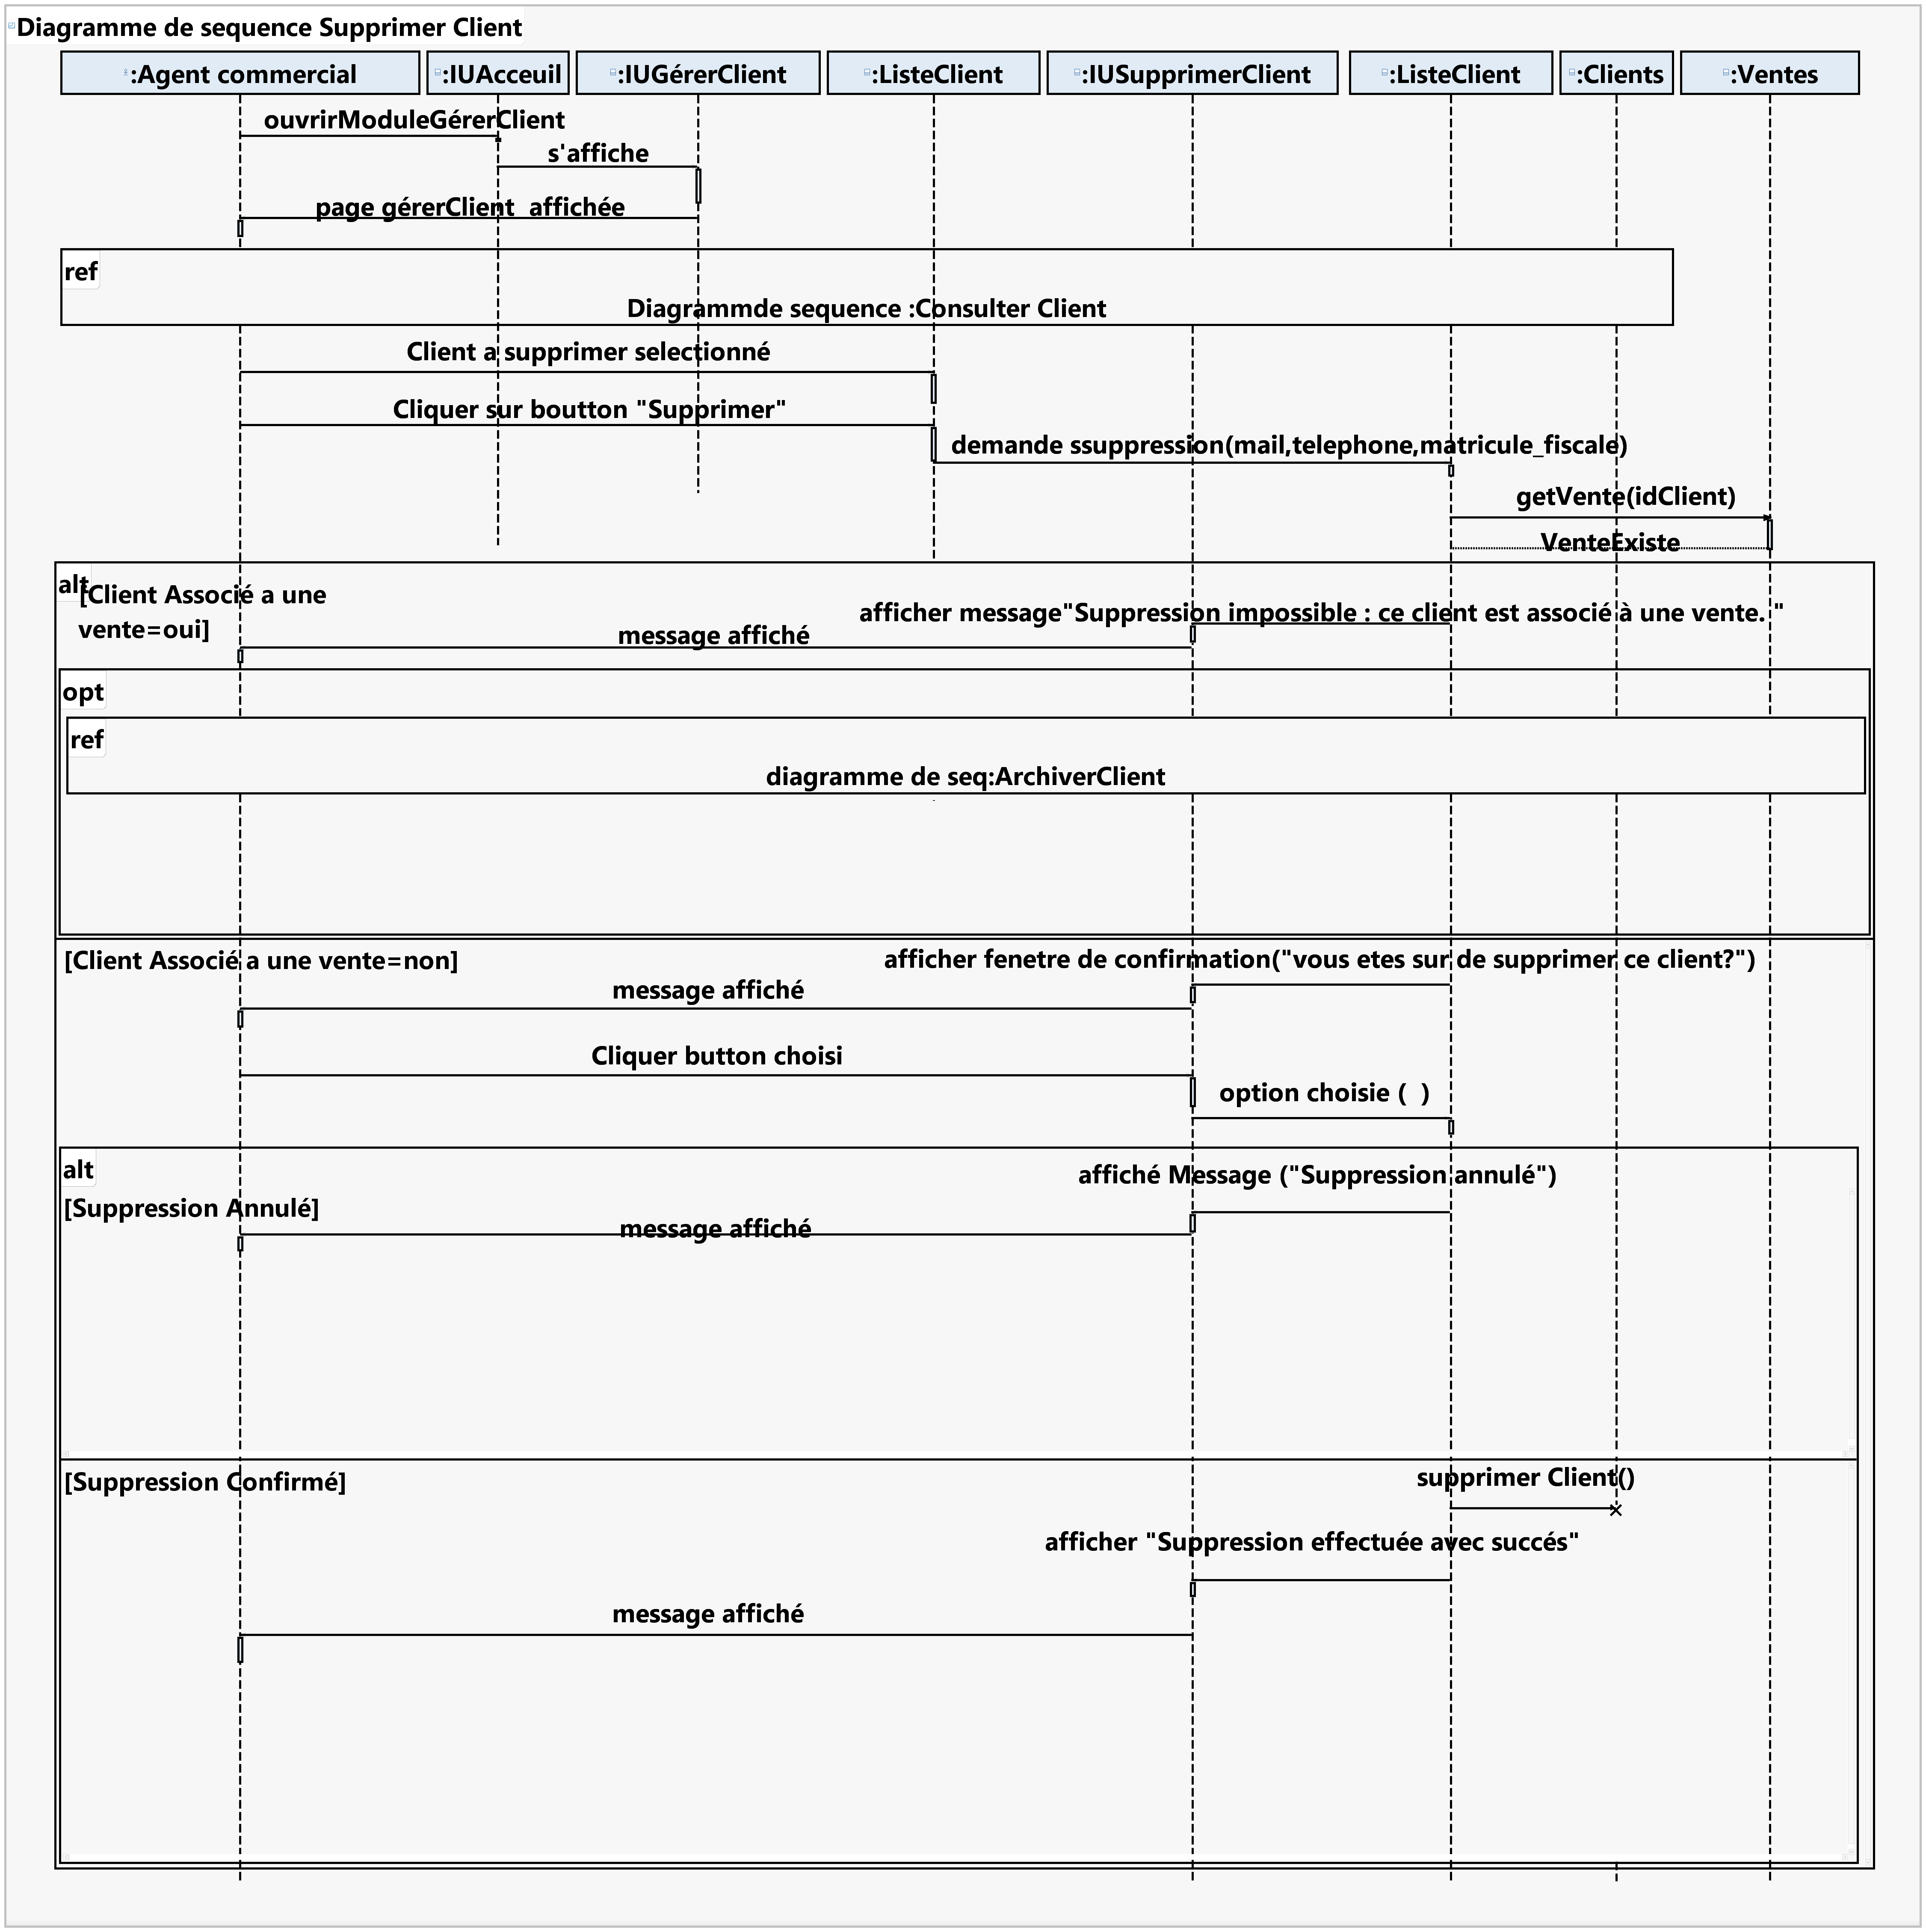
\includegraphics[width=1.15\textwidth, height=0.78\textheight]{images/MC_DiagrammeSéquenceSupprimerClient_2.png}%
  }
  \caption{Diagramme de séquence pour le cas d'utilisation Supprimer Client}
  \label{fig:seqSupprimerClient}
\end{figure}

\needspace{0.88\textheight}
\subsection{Diagramme de Séquence du Cas D'utilisation Consulter Client}

\begin{figure}[H]
  \centering
  \makebox[\textwidth][c]{%
    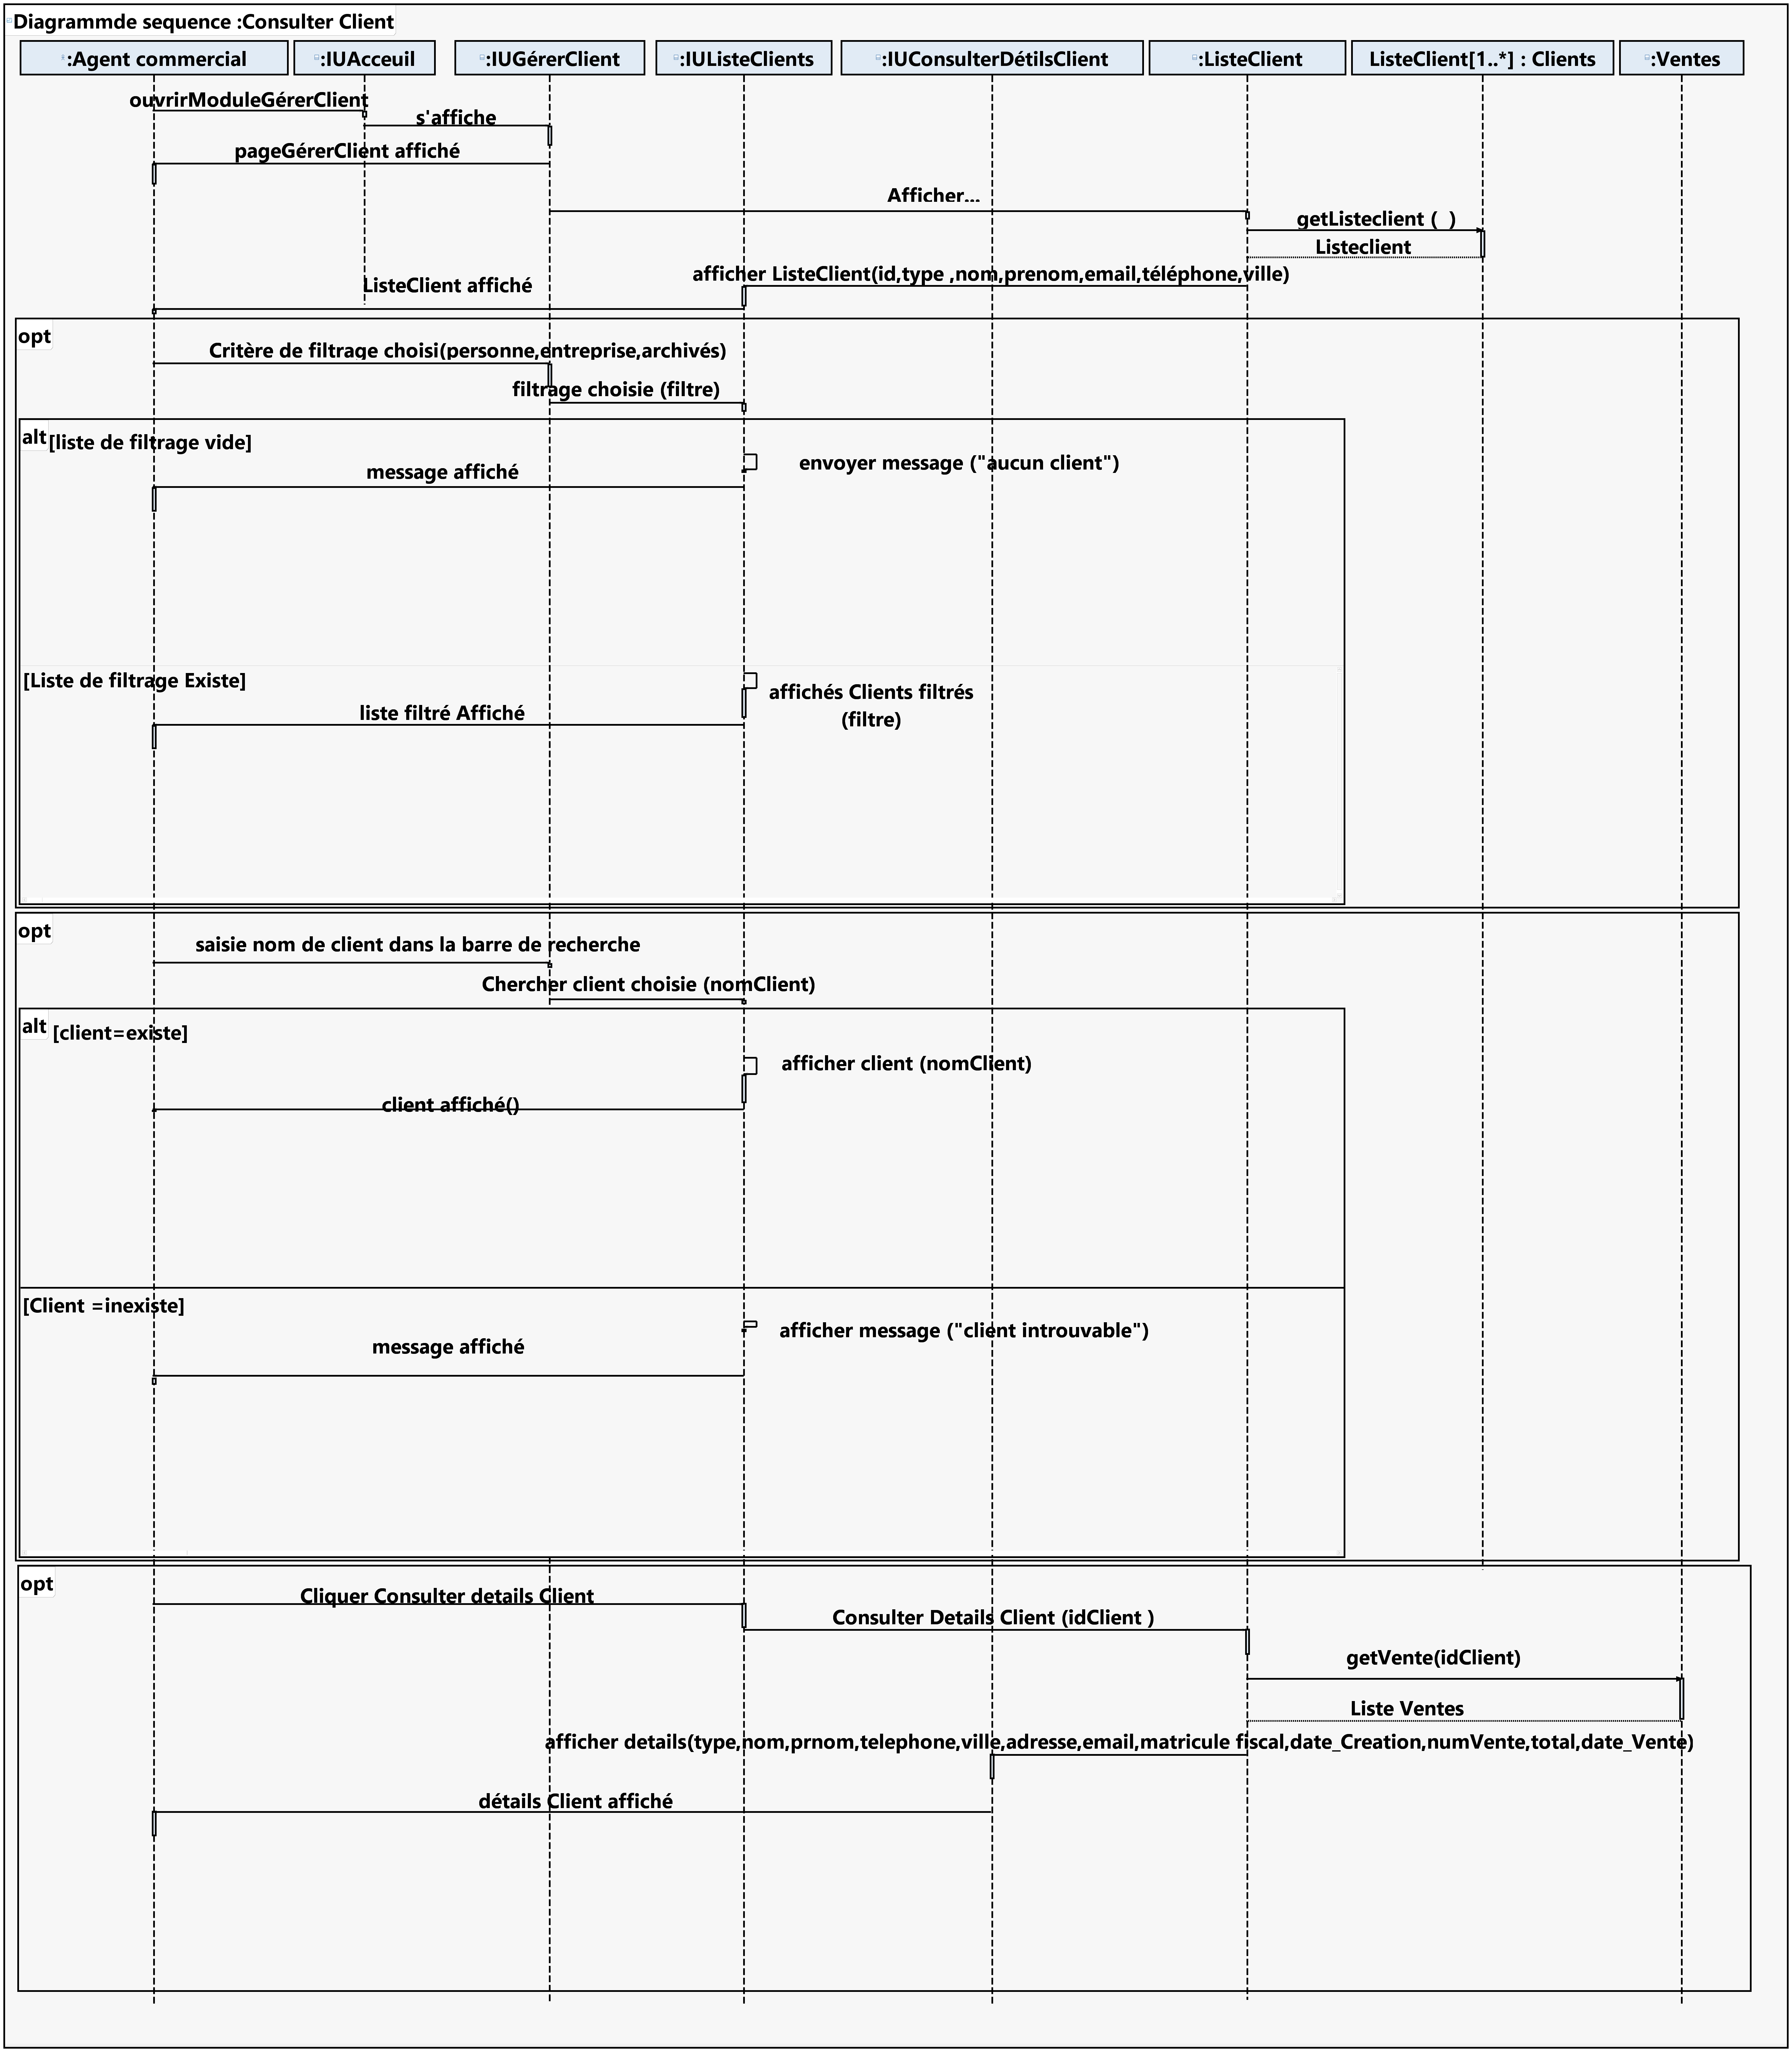
\includegraphics[width=1.15\textwidth, height=0.78\textheight]{images/MC_DiagrammeSéquenceConsulterClient_2.png}%
  }
  \caption{Diagramme de séquence pour le cas d'utilisation Consulter Client}
  \label{fig:seqConsulterClient}
\end{figure}

\needspace{0.88\textheight}
\subsection{Diagramme de Séquence du Cas D'utilisation Archiver Client}

\begin{figure}[H]
  \centering
  \makebox[\textwidth][c]{%
    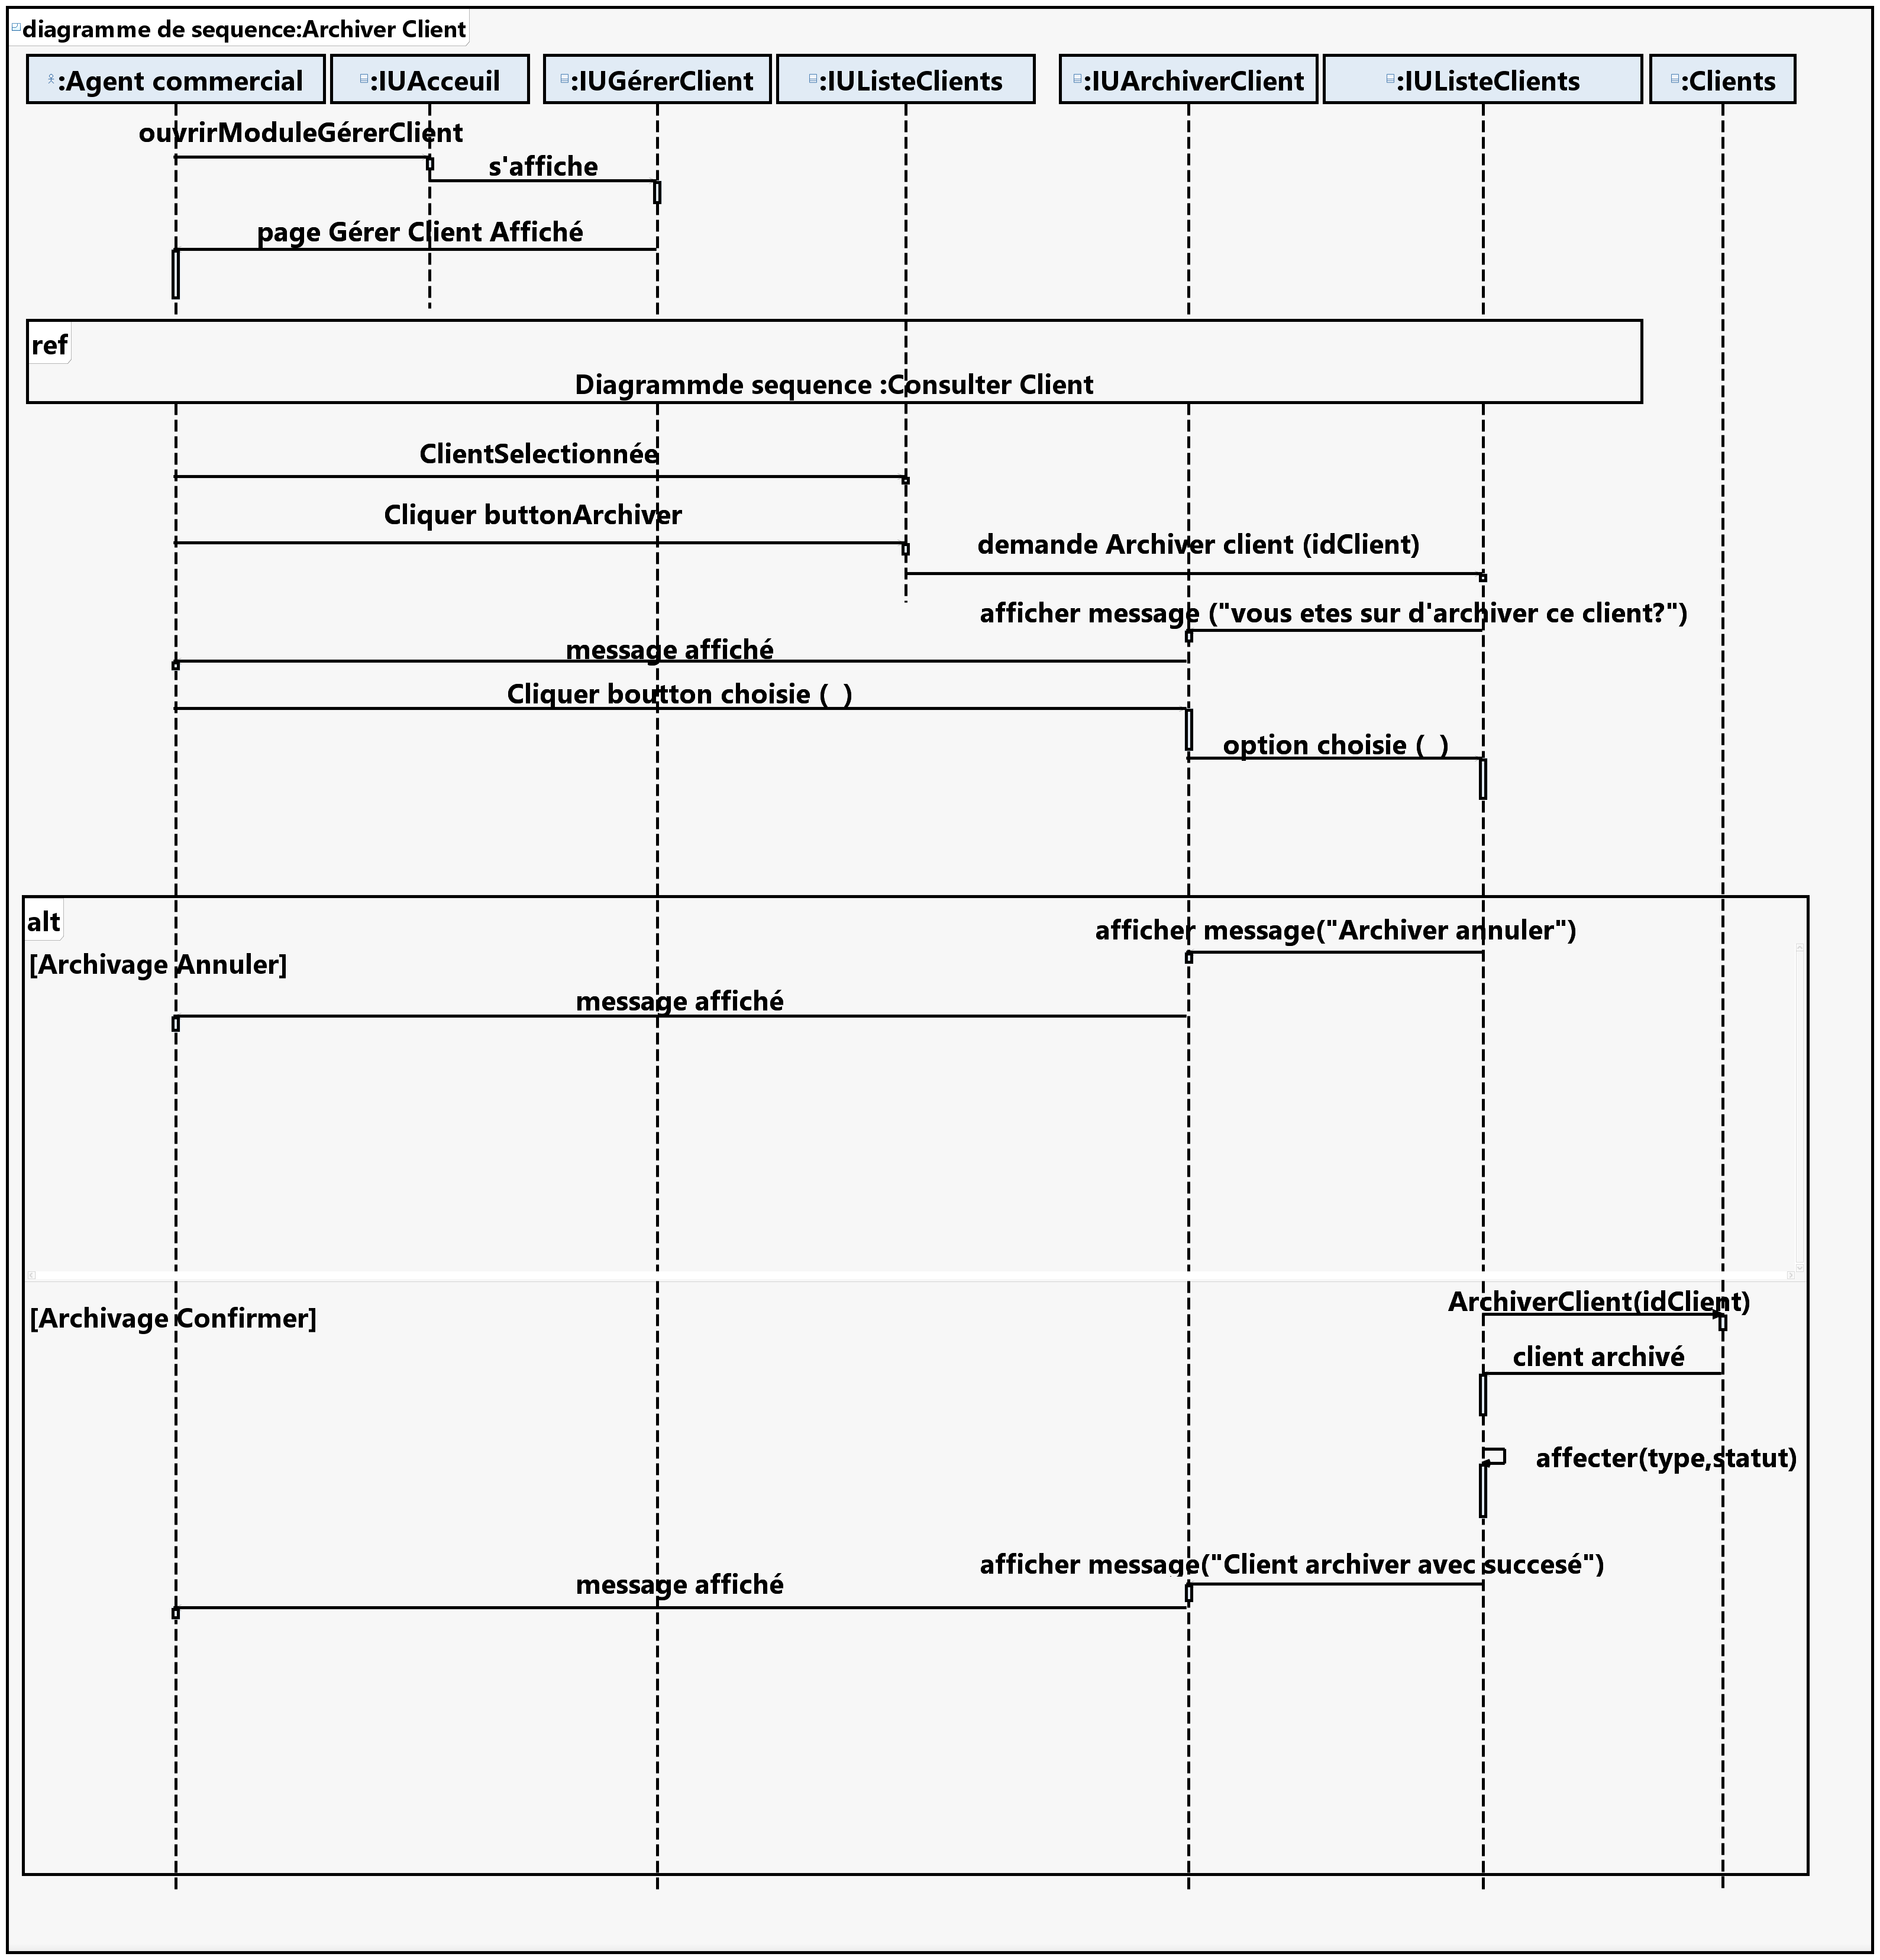
\includegraphics[width=1.15\textwidth, height=0.78\textheight]{images/MC_diagrammedeseqArchiverClient_1.png}%
  }
  \caption{Diagramme de séquence pour le cas d'utilisation Archiver Client}
  \label{fig:seqArchiverClient}
\end{figure}

\needspace{0.88\textheight}
\subsection{Diagramme de Classe du Cas D'utilisation Gérer Clients}

\begin{figure}[H]
  \centering
  \makebox[\textwidth][c]{%
    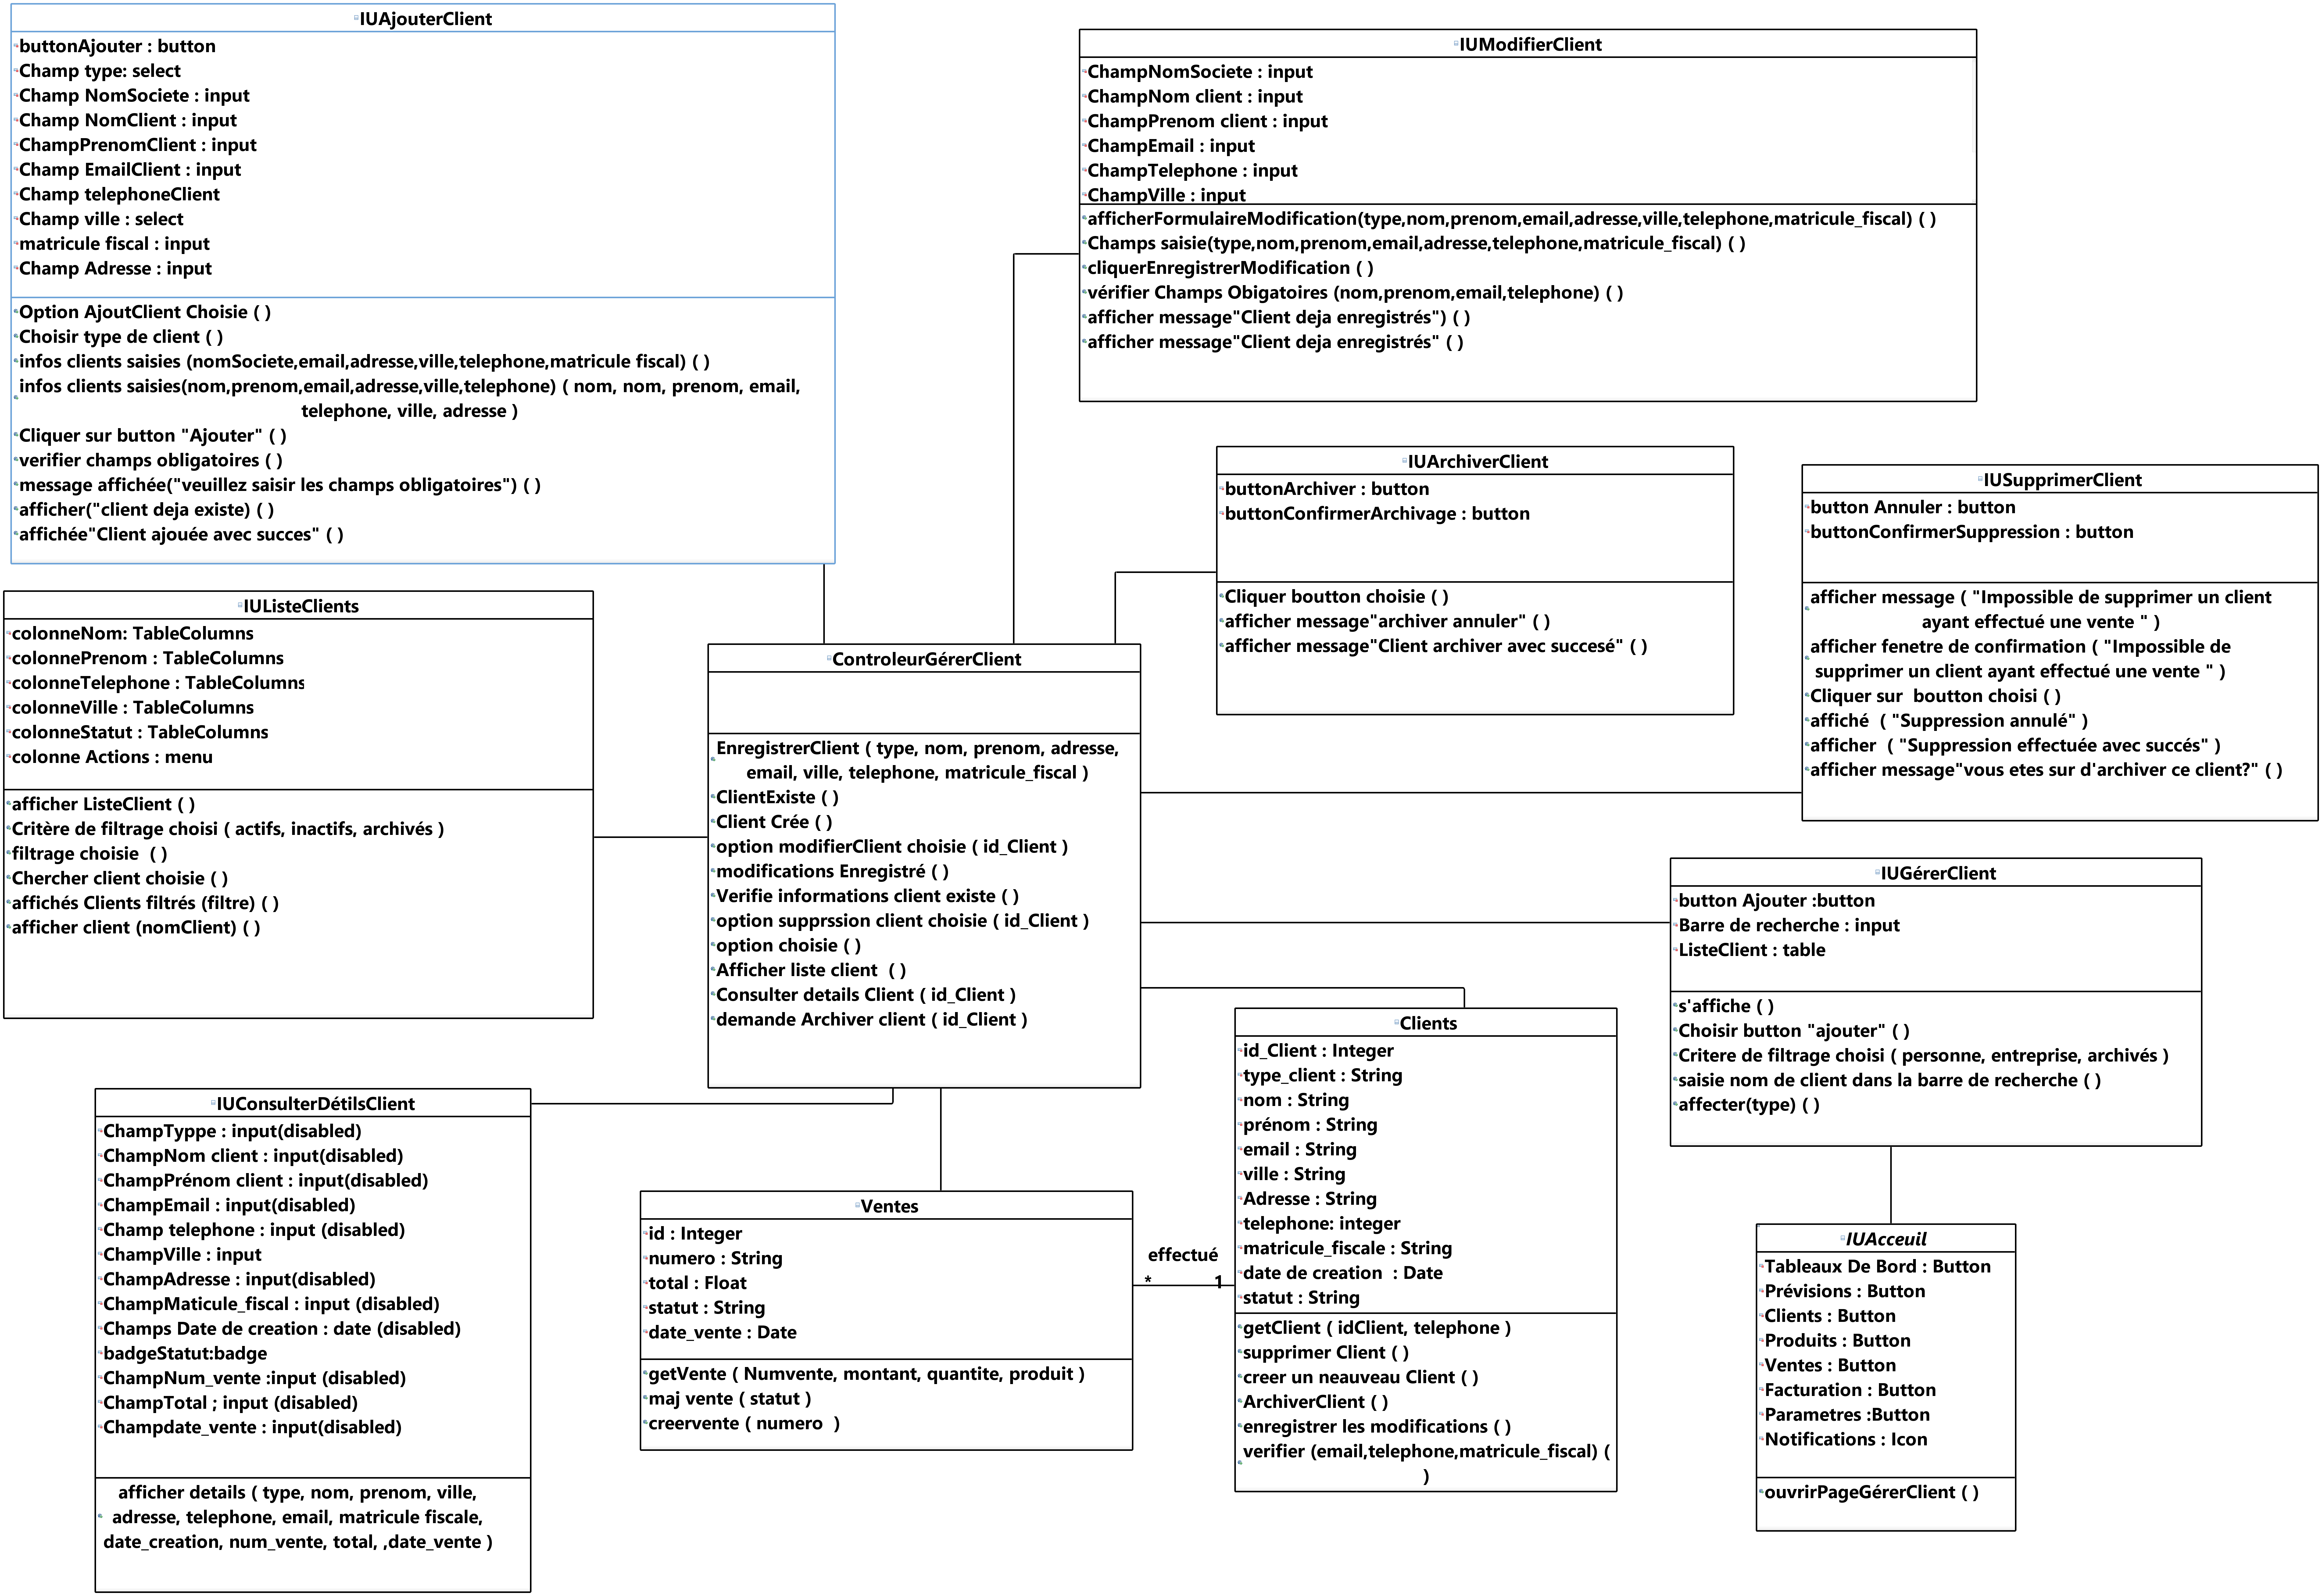
\includegraphics[width=1.15\textwidth, height=0.78\textheight]{images/MC_DiagrammeClasseGererClient_4.png}%
  }
  \caption{Diagramme de classe pour le cas d'utilisation Gérer Clients}
  \label{fig:classeClients}
\end{figure}
\newpage

\section{Conception du Cas D'utilisation Traiter Ventes}

\needspace{0.88\textheight}
\subsection{Traçabilité MCU/MC pour le Cas D'utilisation Traiter Ventes}

\begin{figure}[H]
  \centering
  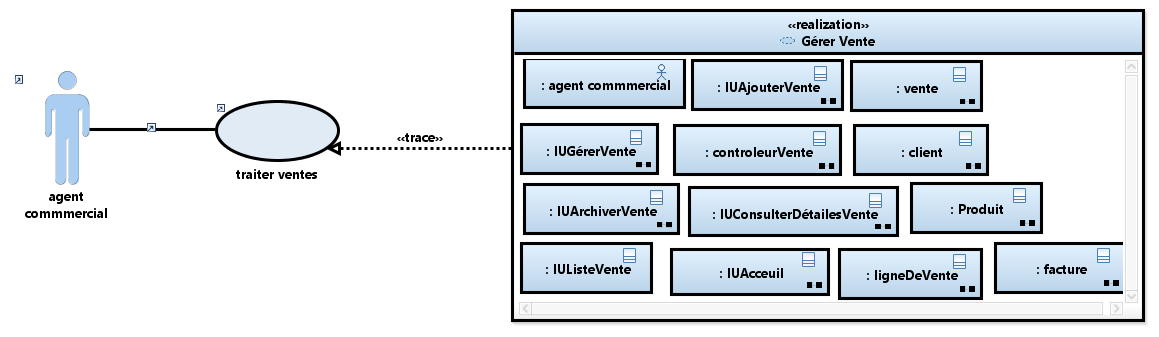
\includegraphics[width=\textwidth]{images/MC_tracabilitéMCMCUVENTE_1.png}
  \caption{Traçabilité MCU/MC pour le cas d'utilisation Traiter Ventes}
\end{figure}

Cette traçabilité montre quels sont les objets instances de classe  participant à la réalisation du cas d'utilisation Traiter Ventes.

L'acteur et Les classes impliquées dans ce diagramme sont les suivantes :

\begin{itemize}[leftmargin=2em, topsep=4pt, itemsep=4pt]
  \item \textbf{Agent Commercial :} l'acteur qui initie les opérations de traitement des ventes
  \item \textbf{IUAccueil :} l'interface principale depuis laquelle l'agent accède à la page de gestion des ventes
  \item \textbf{IUGérerVente :} l'interface principale qui affiche les options de gestion des ventes
  \item \textbf{IUAjouterVente :} l'interface qui permet à l'agent commercial de créer une nouvelle vente en sélectionnant un client et en ajoutant des lignes de produits avec leurs quantités
  \item \textbf{IUArchiverVente :} l'interface qui permet à l'agent commercial de confirmer l'archivage d'une vente
  \item \textbf{IUConsulterDetailsVente :} l'interface qui affiche les détails d'une vente spécifique avec ses lignes de produits
  \item \textbf{IUConsulterListeVente :} l'interface qui affiche la liste des ventes avec les options de recherche et de filtrage
  \item \textbf{ControleurVente :} permet de gérer les flux de contrôle entre l'interface et l'entité
  \newpage
  \item \textbf{Vente :} l'entité du système qui contient la structure de données relative aux ventes
  \item \textbf{Client :} l'entité du système qui contient la structure de données relative aux clients associés à chaque vente
  \item \textbf{Produit :} l'entité du système qui contient la structure de données relative aux produits inclus dans les lignes de vente
  \item \textbf{Facture :} l'entité du système qui contient la structure de données relative aux factures générées à partir des ventes
  \item \textbf{LigneDeVente :} l'entité du système qui contient les données et les  traitements métier relatives aux produits liés à une vente
\end{itemize}

Il est à noter que le CEO peut également effectuer les mêmes opérations de gestion des ventes que l'agent commercial.

\subsection{Diagramme de Séquence du Cas D'utilisation Enregistrer Vente}

\begin{figure}[H]
  \centering
  \makebox[\textwidth][c]{%
    \includegraphics[width=1.15\textwidth, height=0.78\textheight]{images/MC1_DiagrammeSéquenceEnregistrervente_1.png}%
  }
  \caption{Diagramme de séquence pour le cas d'utilisation Enregistrer Vente}
  \label{fig:seqEnregistrerVente}
\end{figure}

\subsection{Diagramme de Séquence du Cas D'utilisation Consulter Vente}

\begin{figure}[H]
  \centering
  \makebox[\textwidth][c]{%
    \includegraphics[width=1.15\textwidth, height=0.78\textheight]{images/MC_DiagrammeSéquenceConsulterVentes_2.png}%
  }
  \caption{Diagramme de séquence pour le cas d'utilisation Consulter Vente}
  \label{fig:seqConsulterVente}
\end{figure}

\needspace{0.88\textheight}
\subsection{Diagramme de Séquence du Cas D'utilisation Archiver Vente}

\begin{figure}[H]
  \centering
  \makebox[\textwidth][c]{%
    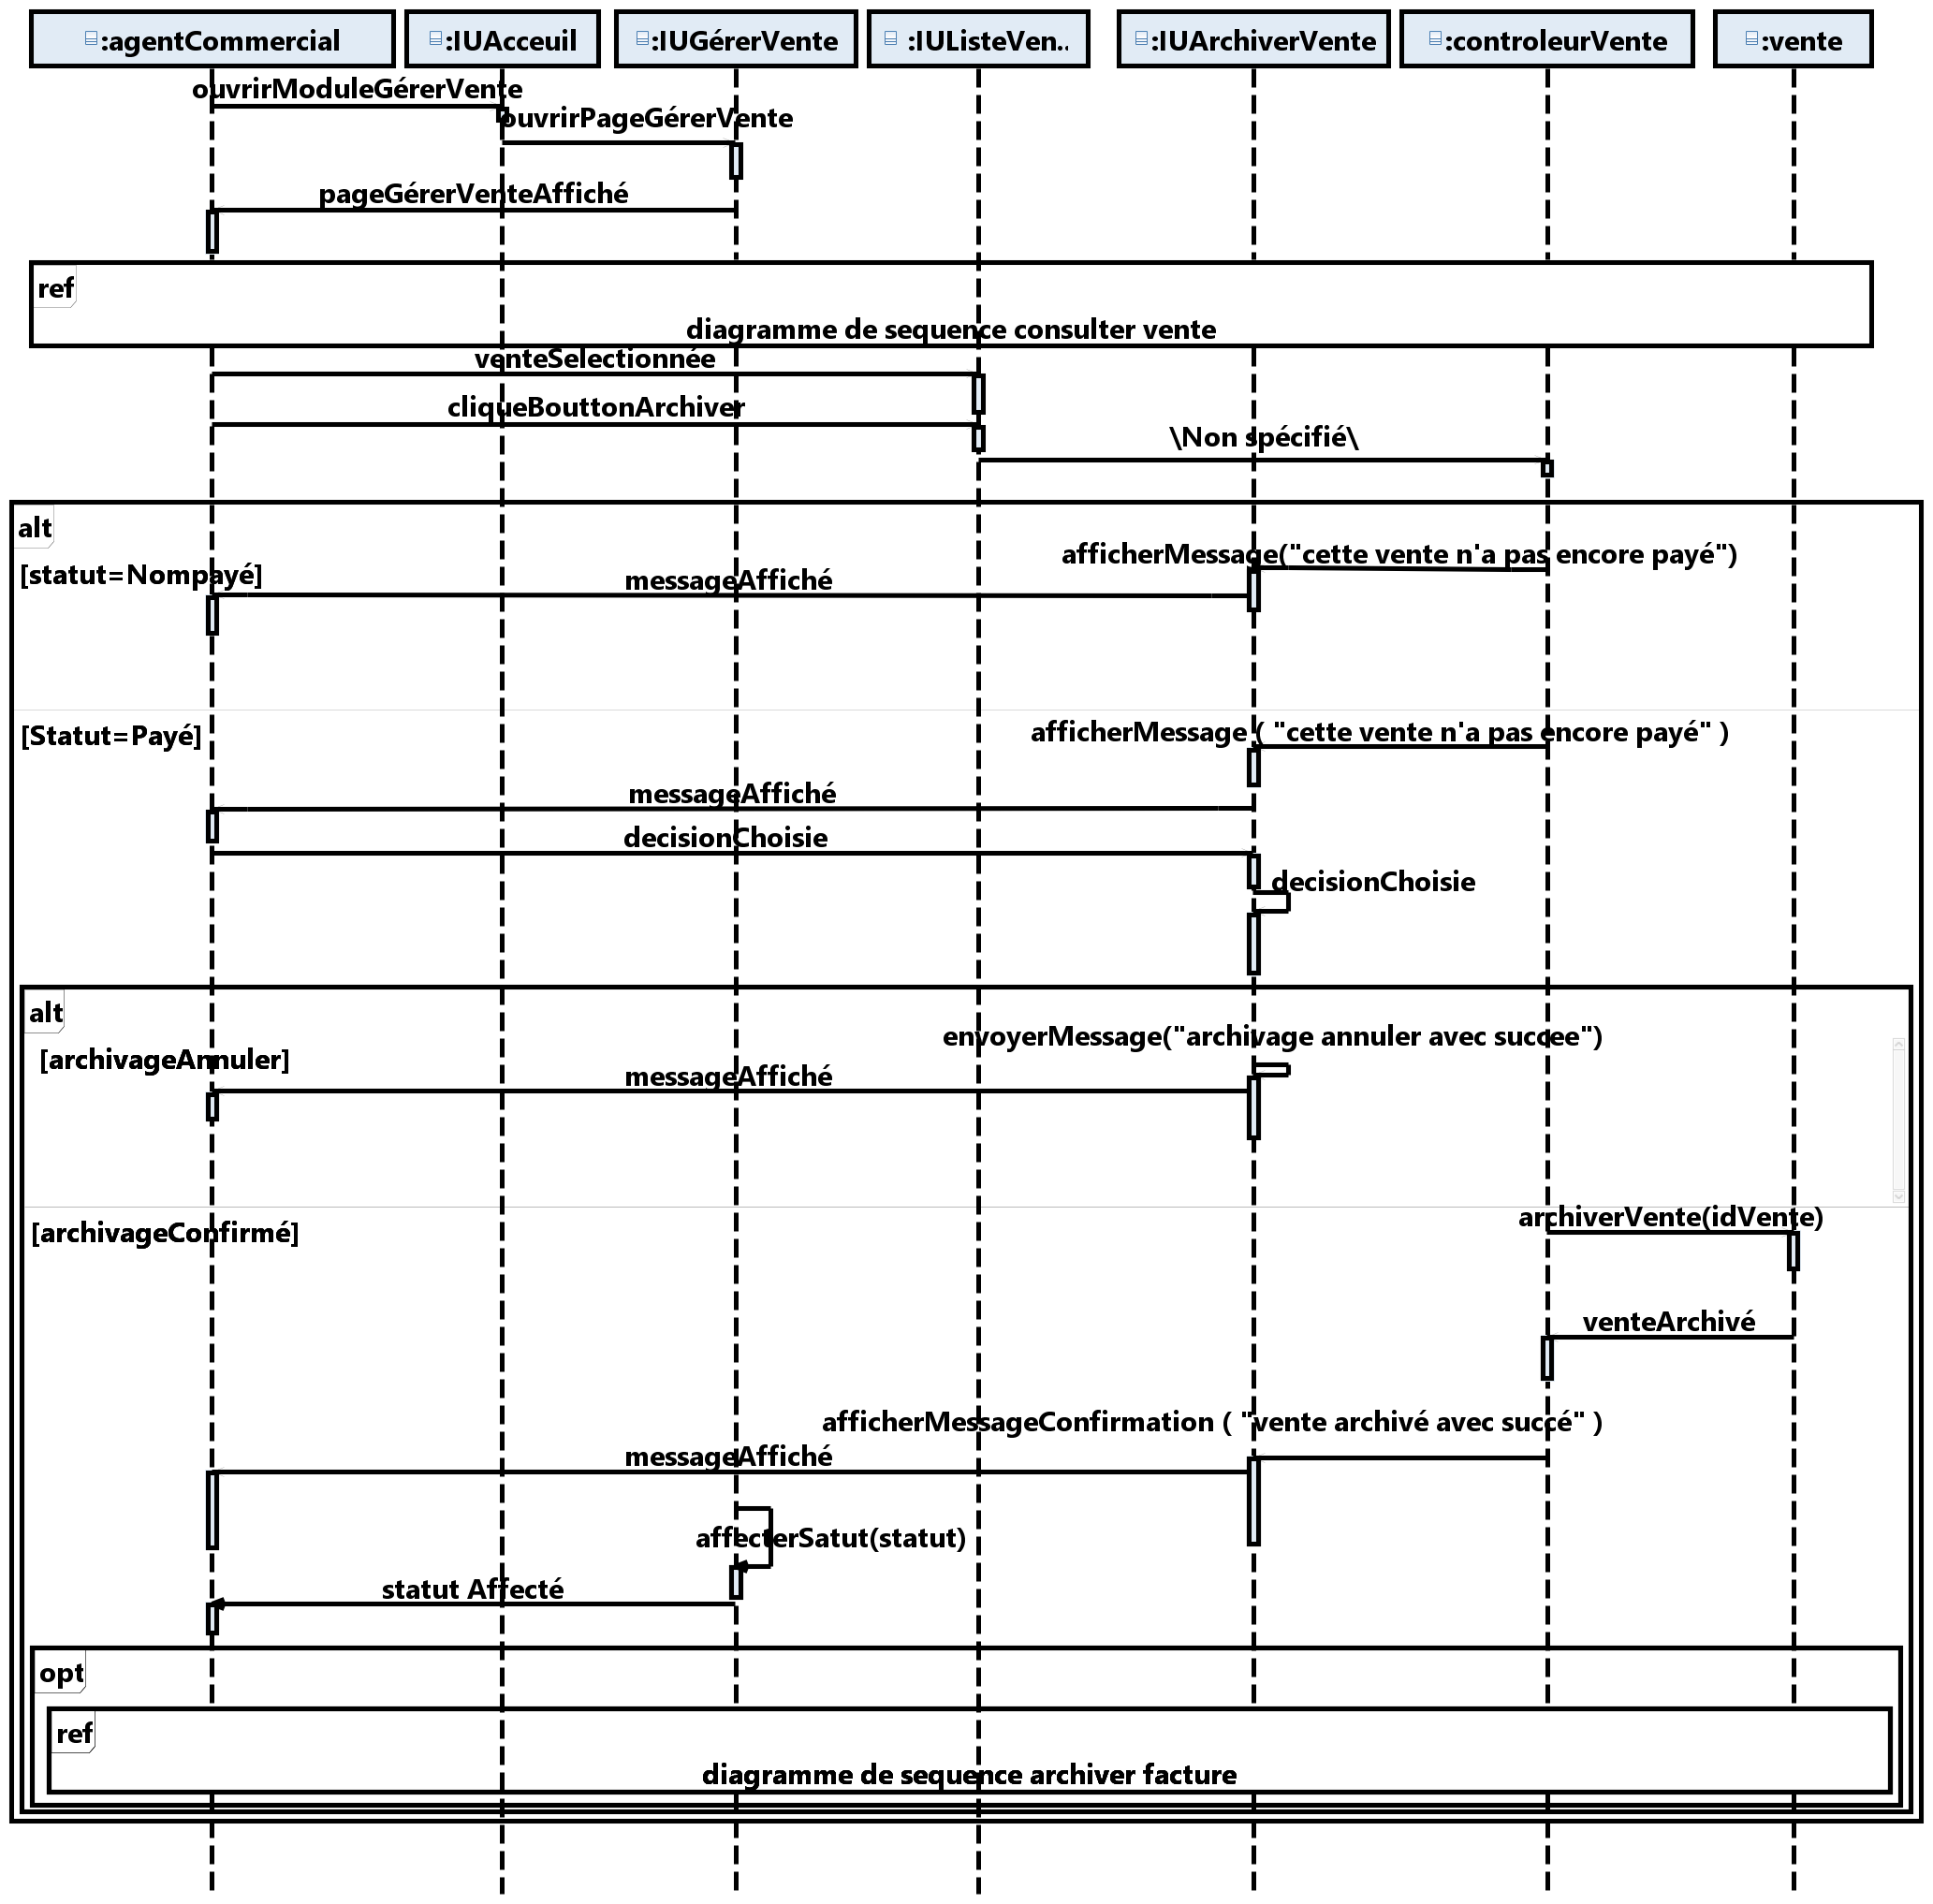
\includegraphics[width=1.15\textwidth, height=0.78\textheight]{images/MC1_DiagrammeSéquenceArchiverVente.png}%
  }
  \caption{Diagramme de séquence pour le cas d'utilisation Archiver Vente}
  \label{fig:seqArchiverVente}
\end{figure}

\needspace{0.88\textheight}
\subsection{Diagramme de Classe du Cas D'utilisation Traiter Ventes}

\begin{figure}[H]
  \centering
  \makebox[\textwidth][c]{%
    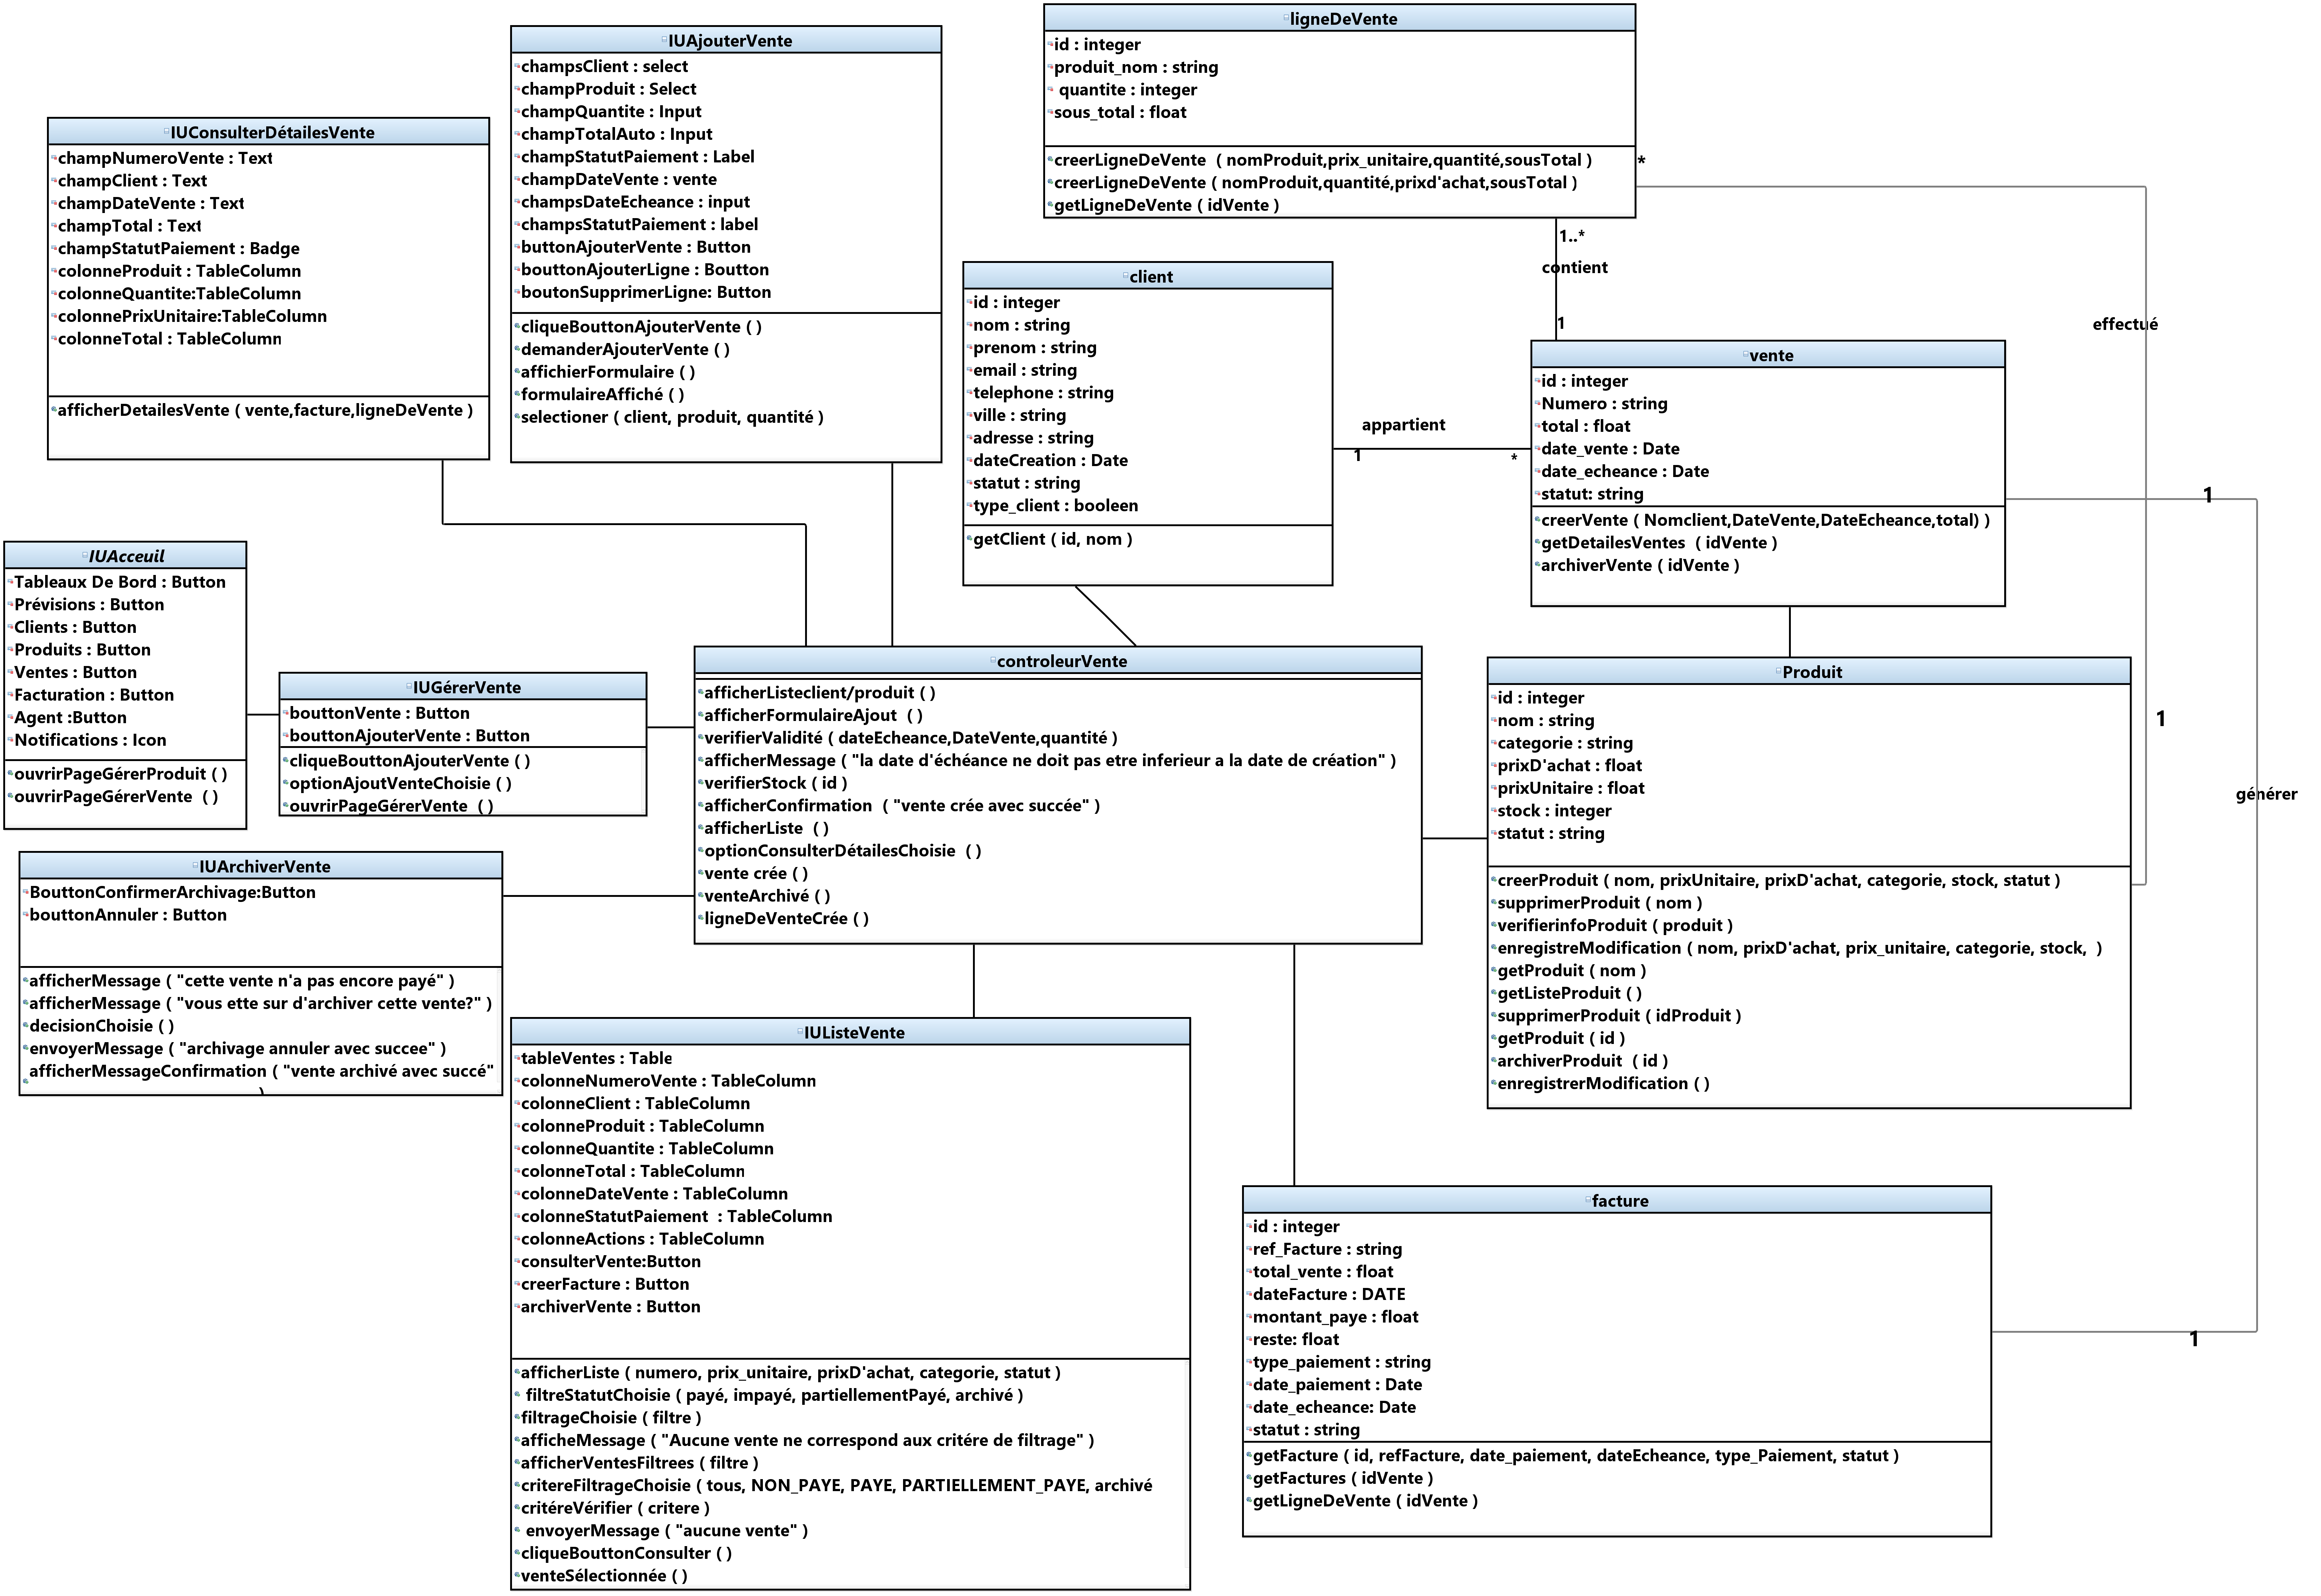
\includegraphics[width=1.15\textwidth, height=0.78\textheight]{images/MC1_DiagrammeDeClasseGérerVente.png}%
  }
  \caption{Diagramme de classe pour le cas d'utilisation Traiter Ventes}
  \label{fig:classeVentes}
\end{figure}

\clearpage
\section{Conception du Cas D'utilisation Gérer Factures}

\subsection{Traçabilité MCU/MC pour le Cas D'utilisation Gérer Factures}

\begin{figure}[H]
  \centering
  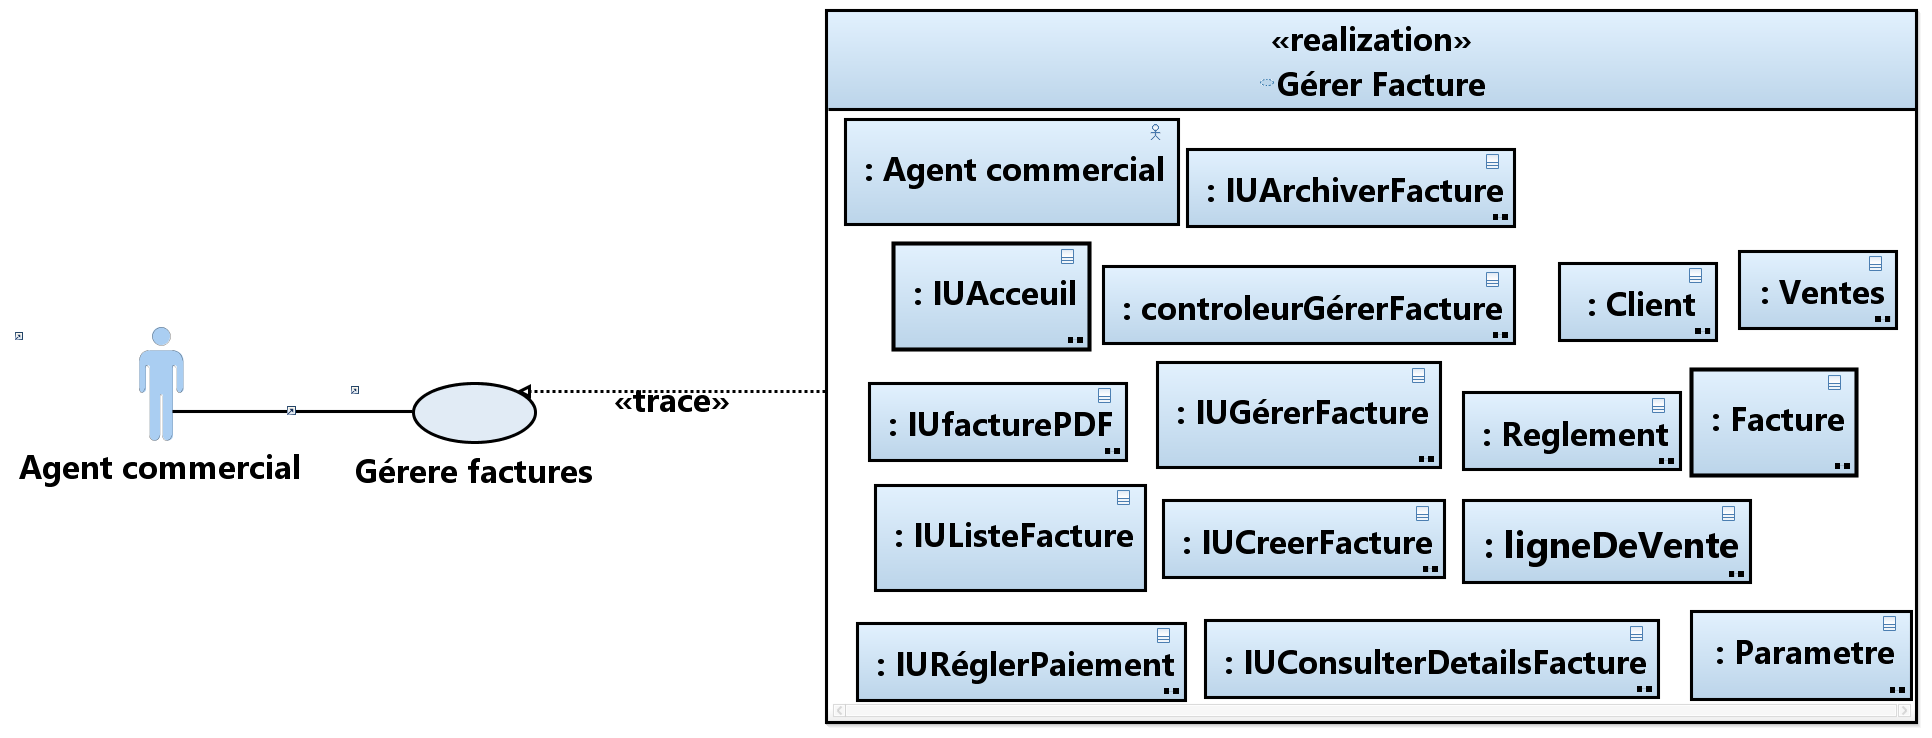
\includegraphics[width=\textwidth]{images/MC_tracabiliteMCUMCGérerFacture_2.png}
  \caption{Traçabilité MCU/MC pour le cas d'utilisation Gérer Factures}
\end{figure}

Cette traçabilité montre quels sont les objets instances de classe participant à la réalisation du cas d'utilisation Gérer Factures.

L'acteur et les classes impliquées dans ce diagramme sont les suivants :

\begin{itemize}[leftmargin=2em, topsep=4pt, itemsep=4pt]
  \item \textbf{Agent Commercial :} l'acteur qui initie les opérations de gestion des factures
  \item \textbf{IUAccueil :} l'interface principale depuis laquelle l'agent accède à la page de gestion des factures
  \item \textbf{IUGérerFacture :} l'interface principale qui affiche les options de gestion des factures
  \item \textbf{IUCreerFacture :} l'interface qui permet à l'agent commercial de créer une nouvelle facture à partir d'une vente
  \item \textbf{IUListeFacture :} l'interface qui affiche la liste des factures avec les options de recherche et de filtrage par statut
  \item \textbf{IUConsulterDetailsFacture :} l'interface qui permet à l'agent commercial de visualiser les informations détaillées d'une facture sélectionnée
  \item \textbf{IURéglerPaiement :} l'interface qui permet à l'agent commercial d'ajouter un règlement à une facture
  \item \textbf{IUArchiverFacture :} l'interface qui permet à l'agent commercial de confirmer l'archivage d'une facture
  \item \textbf{IUFacturePDF :} l'interface qui permet à l'agent commercial de générer et télécharger la facture au format PDF
  \item \textbf{ControleurGérerFacture :} permet de gérer les flux de contrôle entre l'interface et les entités facture, vente, client et règlement
  \item \textbf{Facture :} l'entité du système qui contient la structure de données relative aux factures
  \item \textbf{Règlement :} l'entité qui représente les versements effectués sur une facture
  \item \textbf{Paramètre :} l'entité qui représente les paramètres de la société tels que (société\_nom, adresse, ville, téléphone)
  \item \textbf{LigneDeVente :} l'entité du système qui contient les données et les traitements métier relatives aux produits liés à une vente
  \item \textbf{Vente :} l'entité associée à la facture représentant la vente d'origine
  \item \textbf{Client :} l'entité qui représente le client associé à la facture
\end{itemize}

\needspace{0.88\textheight}
\subsection{Diagramme de Séquence du Cas D'utilisation Créer Facture Via Facture}

\begin{figure}[H]
  \centering
  \makebox[\textwidth][c]{%
    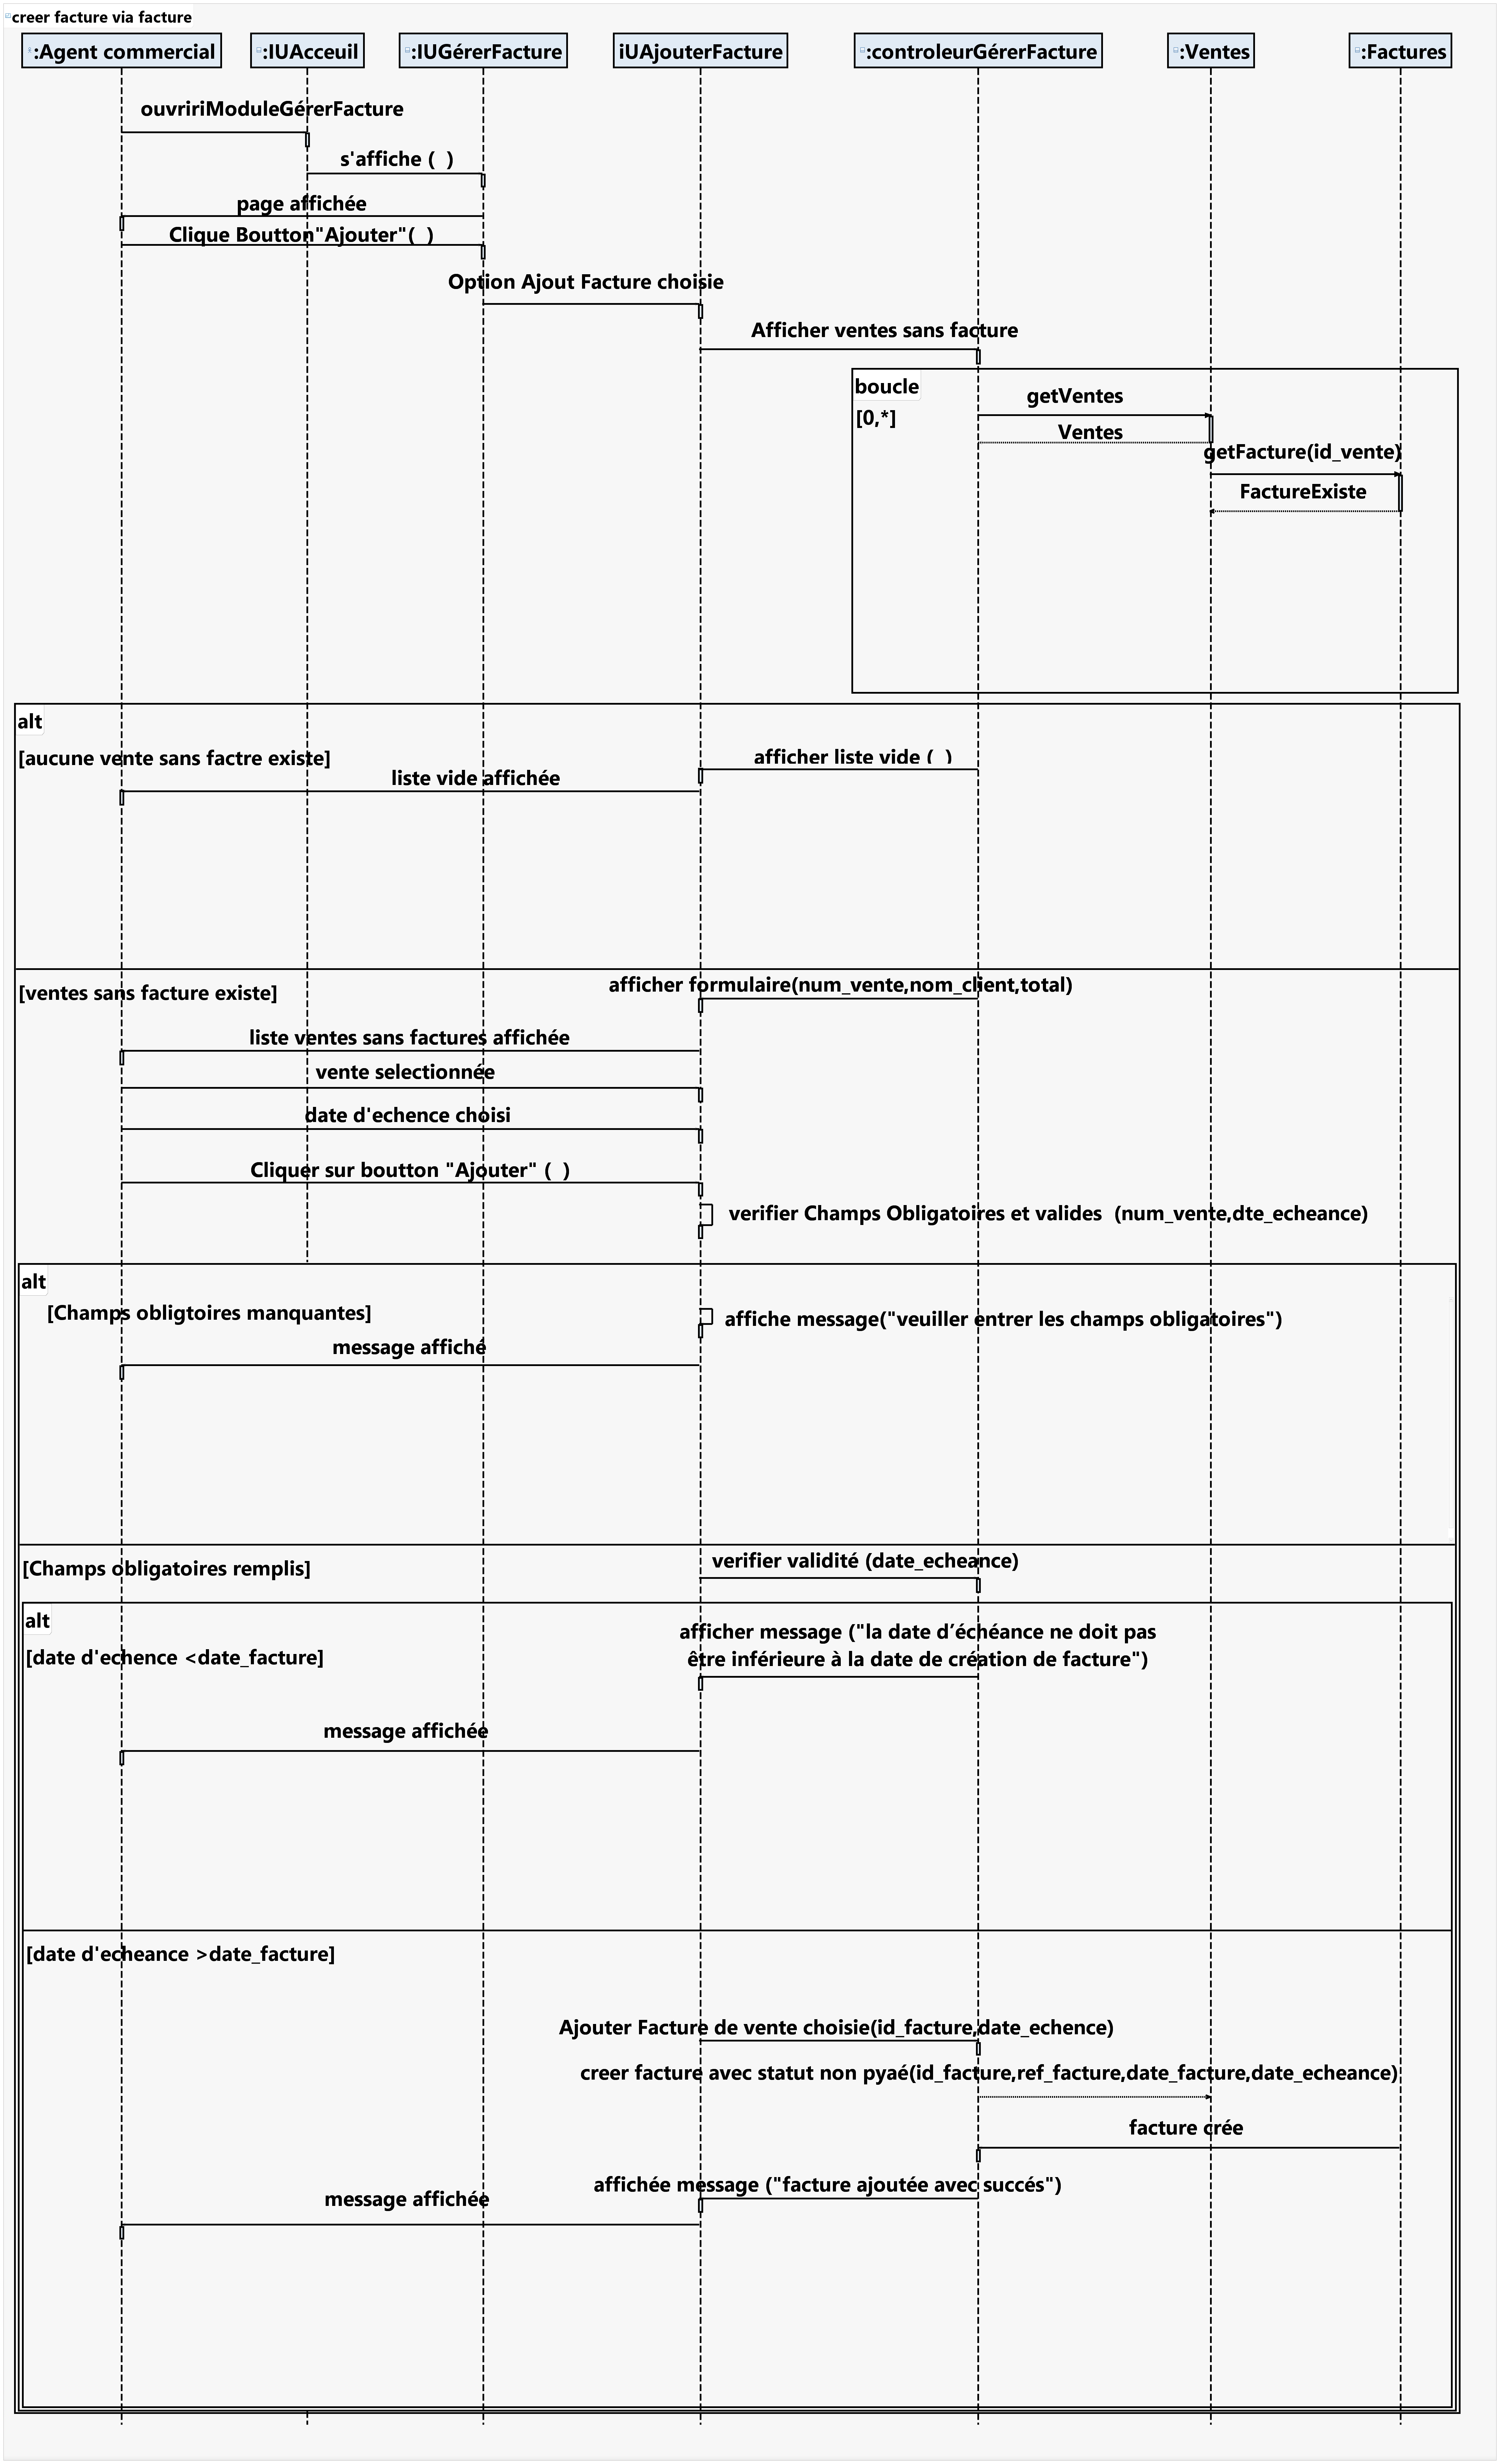
\includegraphics[width=1.15\textwidth, height=0.78\textheight]{images/MC_DiagrammeSéquenceCreerFactureviafacture_2.png}%
  }
  \caption{Diagramme de séquence pour le cas d'utilisation Créer Facture Via Facture}
  \label{fig:seqCreerFactureViaFacture}
\end{figure}

\needspace{0.88\textheight}
\subsection{Diagramme de Séquence du Cas D'utilisation Créer Facture Via Vente}

\begin{figure}[H]
  \centering
  \makebox[\textwidth][c]{%
    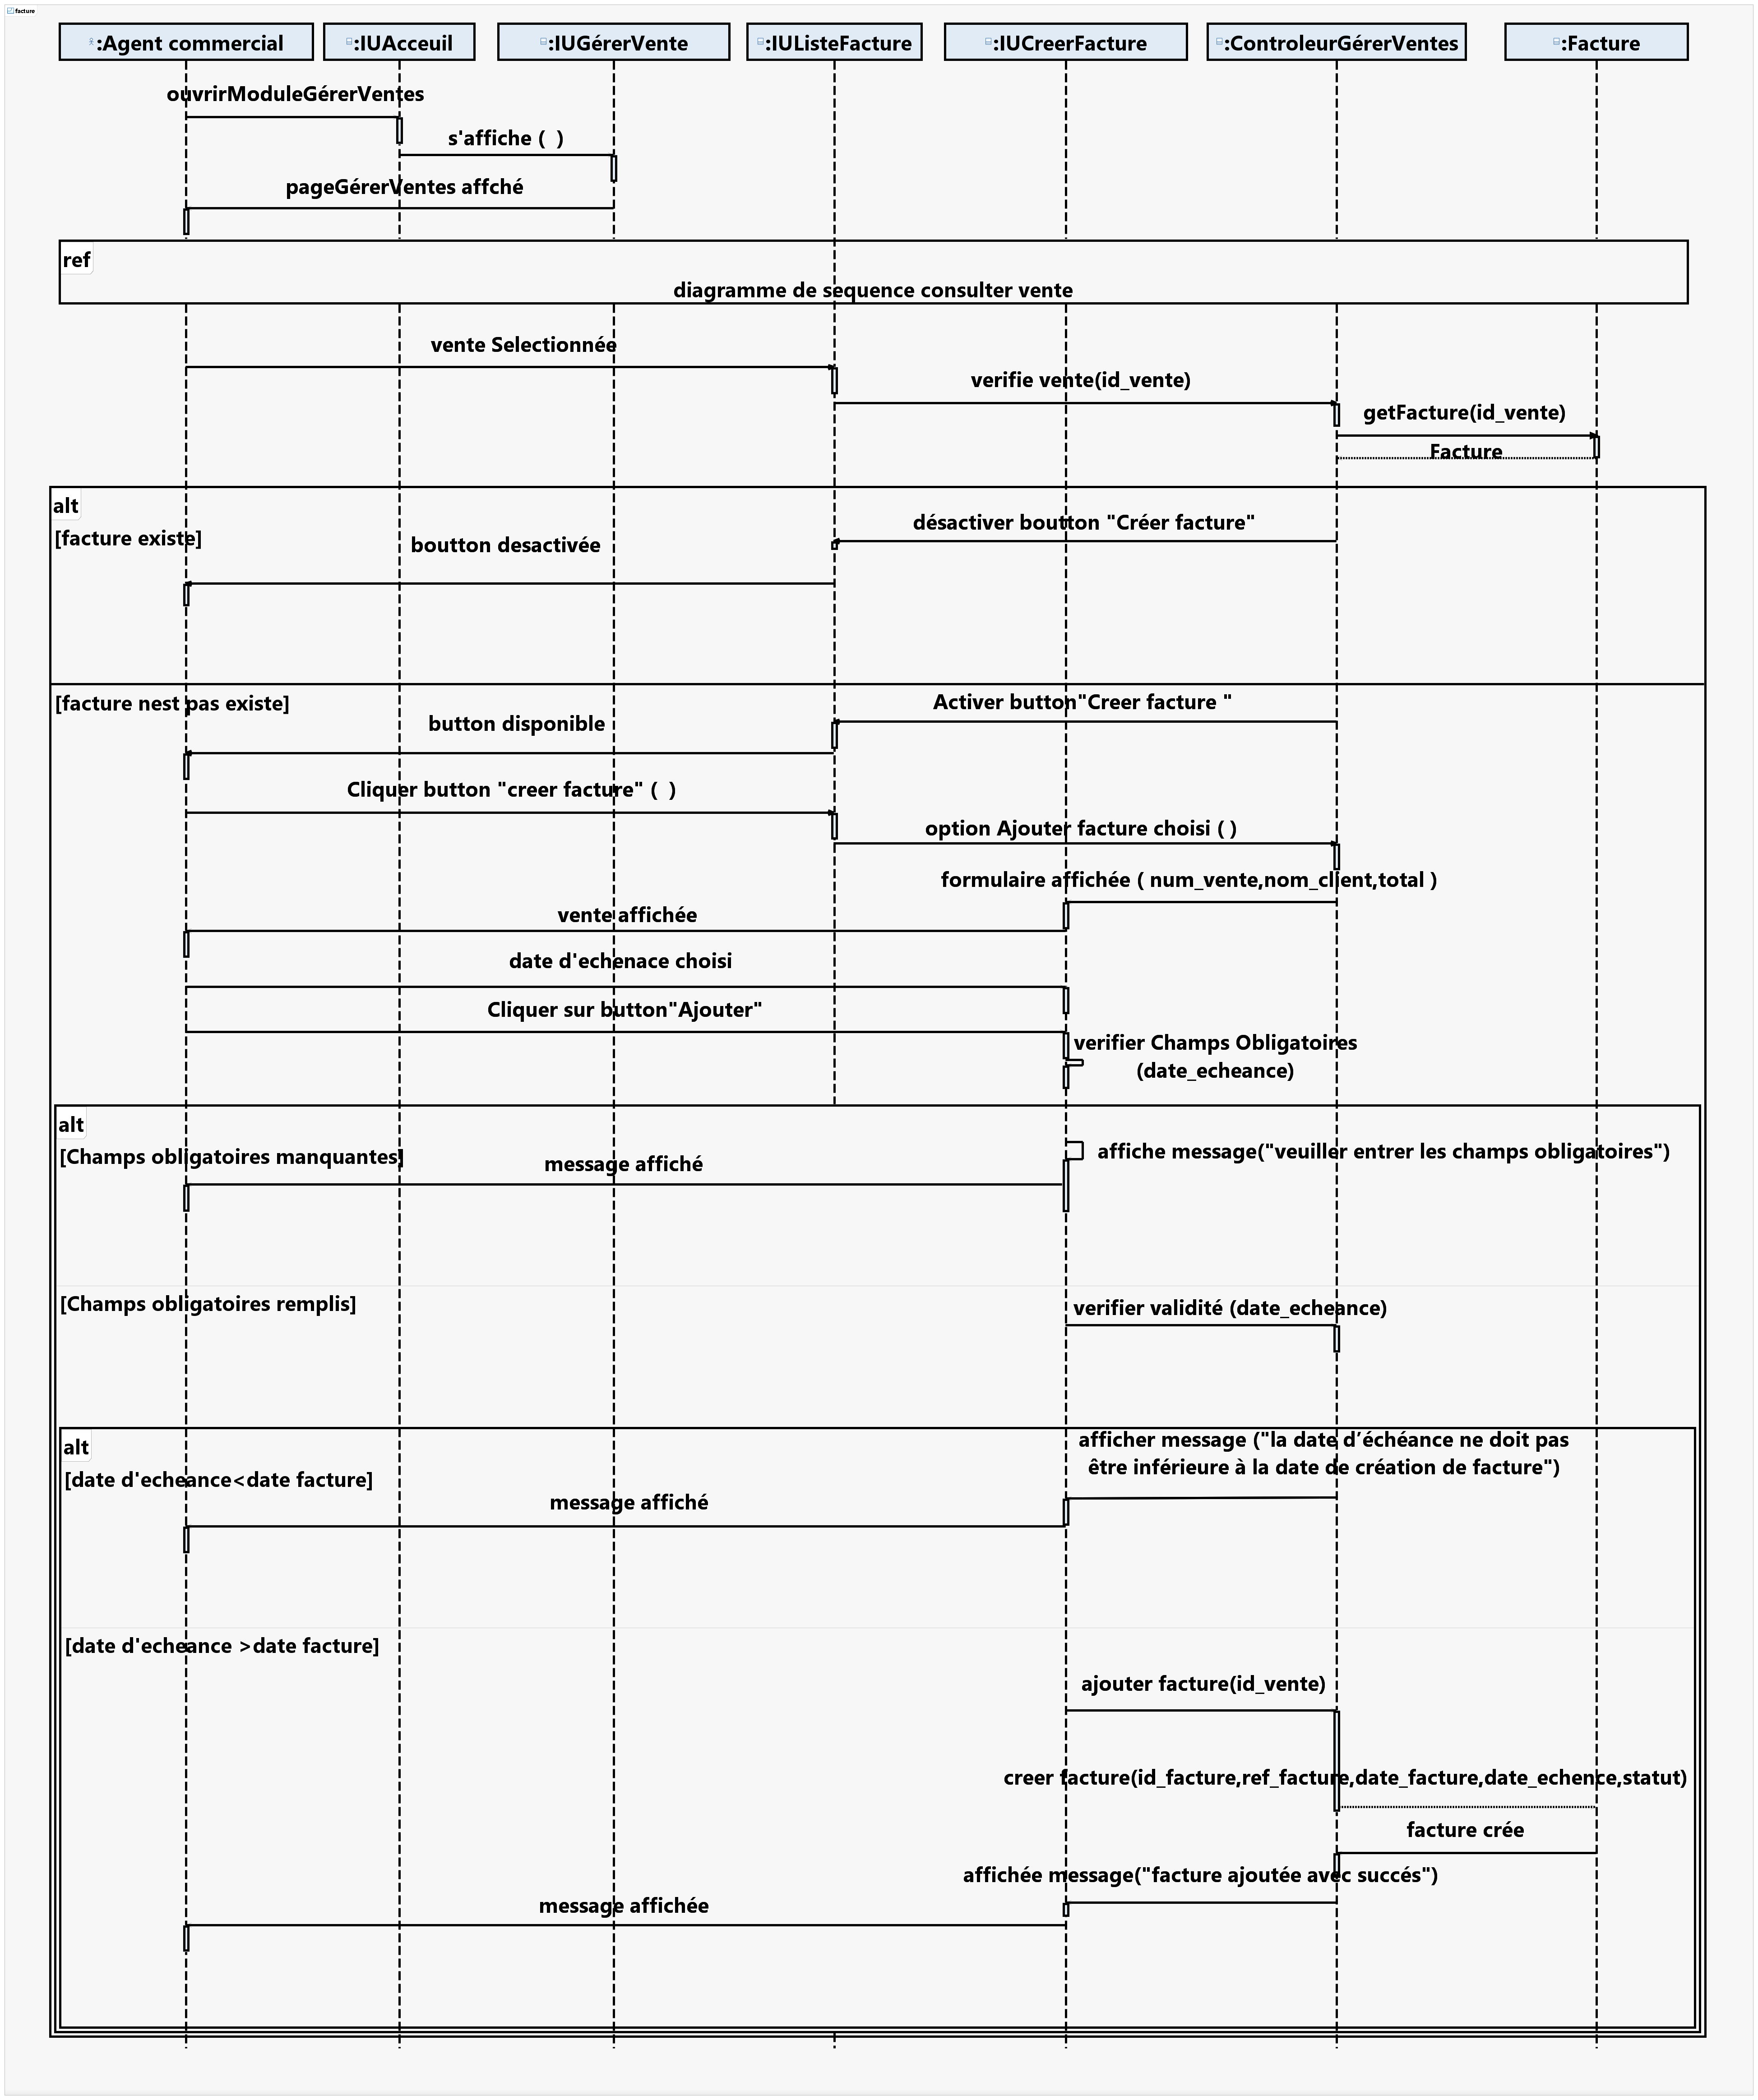
\includegraphics[width=1.15\textwidth, height=0.78\textheight]{images/MC_DiagrammeSéquencecreerfactureviaventes.png}%
  }
  \caption{Diagramme de séquence pour le cas d'utilisation Créer Facture Via Vente}
  \label{fig:seqCreerFactureViaVente}
\end{figure}

\needspace{0.88\textheight}
\subsection{Diagramme de Séquence du Cas D'utilisation Consulter Facture}

\begin{figure}[H]
  \centering
  \makebox[\textwidth][c]{%
    \includegraphics[width=1.15\textwidth, height=0.78\textheight]{images/MC_DiagrammeSéquenceConsulterFacture_4.png}%
  }
  \caption{Diagramme de séquence pour le cas d'utilisation Consulter Facture}
  \label{fig:seqConsulterFacture}
\end{figure}

\needspace{0.88\textheight}
\subsection{Diagramme de Séquence du Cas D'utilisation Enregistrer Règlement}

\begin{figure}[H]
  \centering
  \makebox[\textwidth][c]{%
    \includegraphics[width=1.15\textwidth, height=0.78\textheight]{images/MC_DiagrammeSéquenceEnregistrerRèglement_2.png}%
  }
  \caption{Diagramme de séquence pour le cas d'utilisation Enregistrer Règlement}
  \label{fig:seqEnregistrerReglement}
\end{figure}

\needspace{0.88\textheight}
\subsection{Diagramme de Séquence du Cas D'utilisation Archiver Facture}

\begin{figure}[H]
  \centering
  \makebox[\textwidth][c]{%
    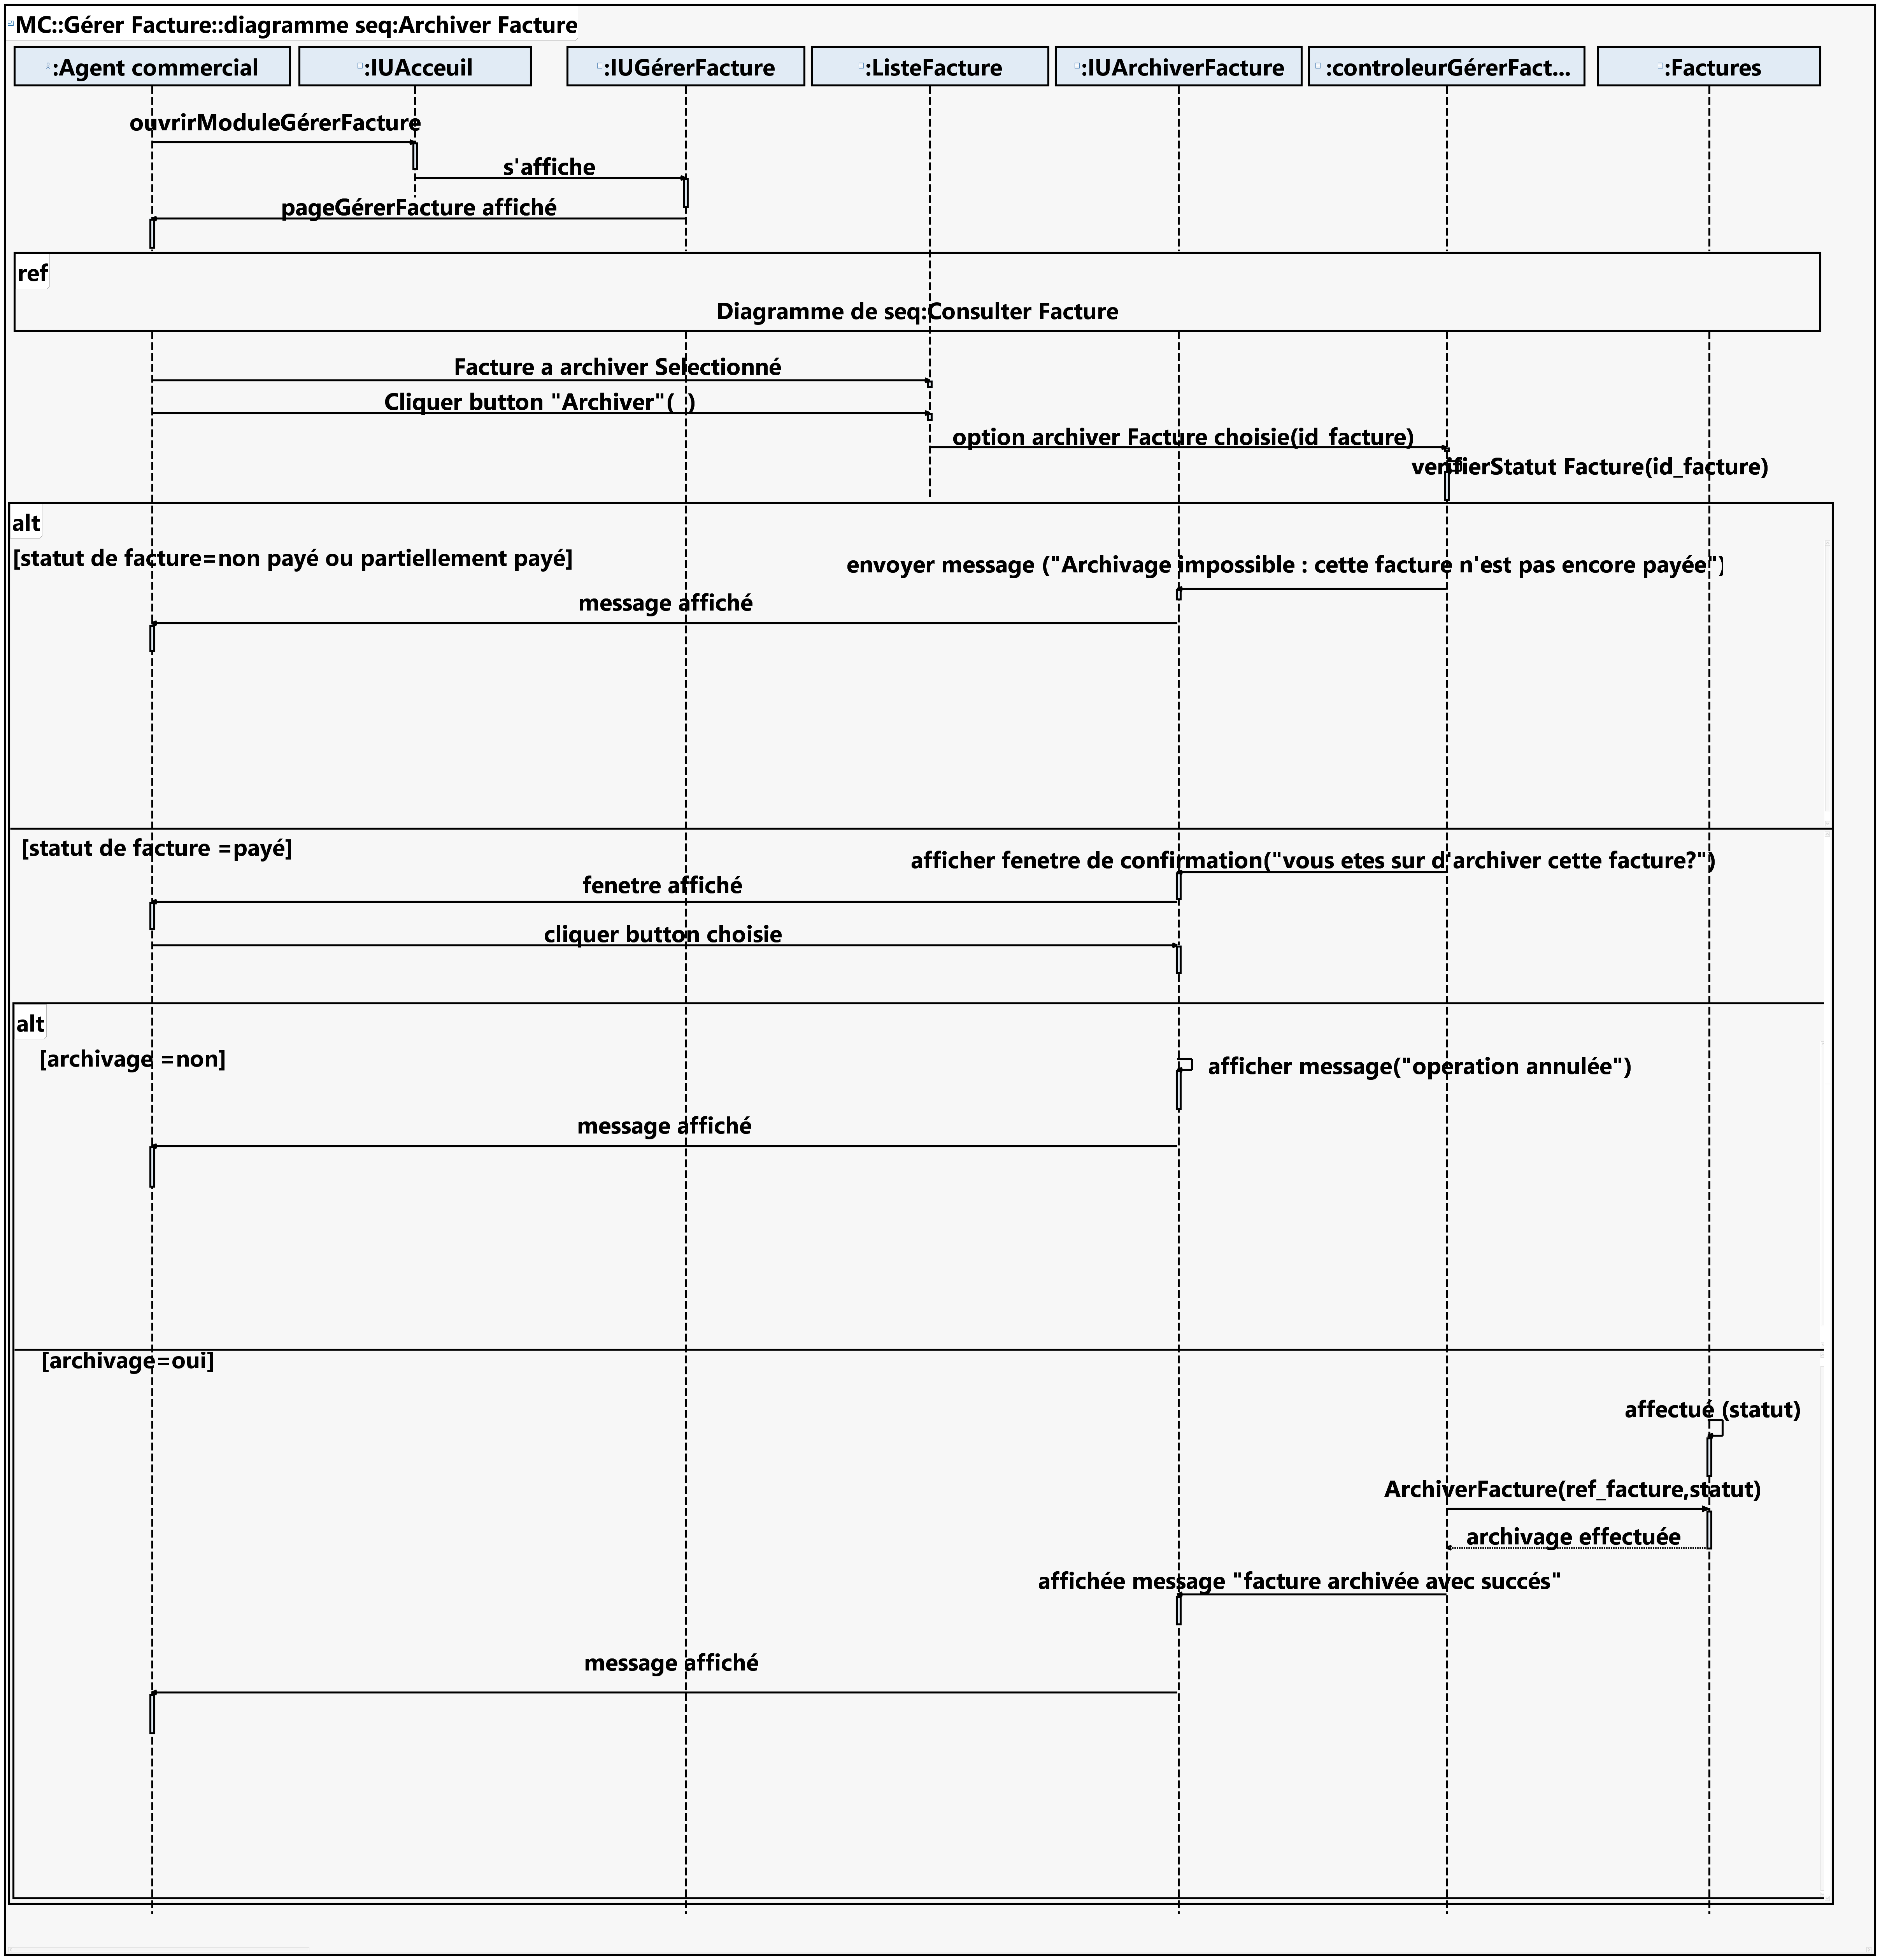
\includegraphics[width=1.15\textwidth, height=0.78\textheight]{images/MC_DiagrammeSéquenceArchiverFacture_2.png}%
  }
  \caption{Diagramme de séquence pour le cas d'utilisation Archiver Facture}
  \label{fig:seqArchiverFacture}
\end{figure}

\needspace{0.88\textheight}
\subsection{Diagramme de Séquence du Cas D'utilisation Imprimer Facture}

\begin{figure}[H]
  \centering
  \makebox[\textwidth][c]{%
    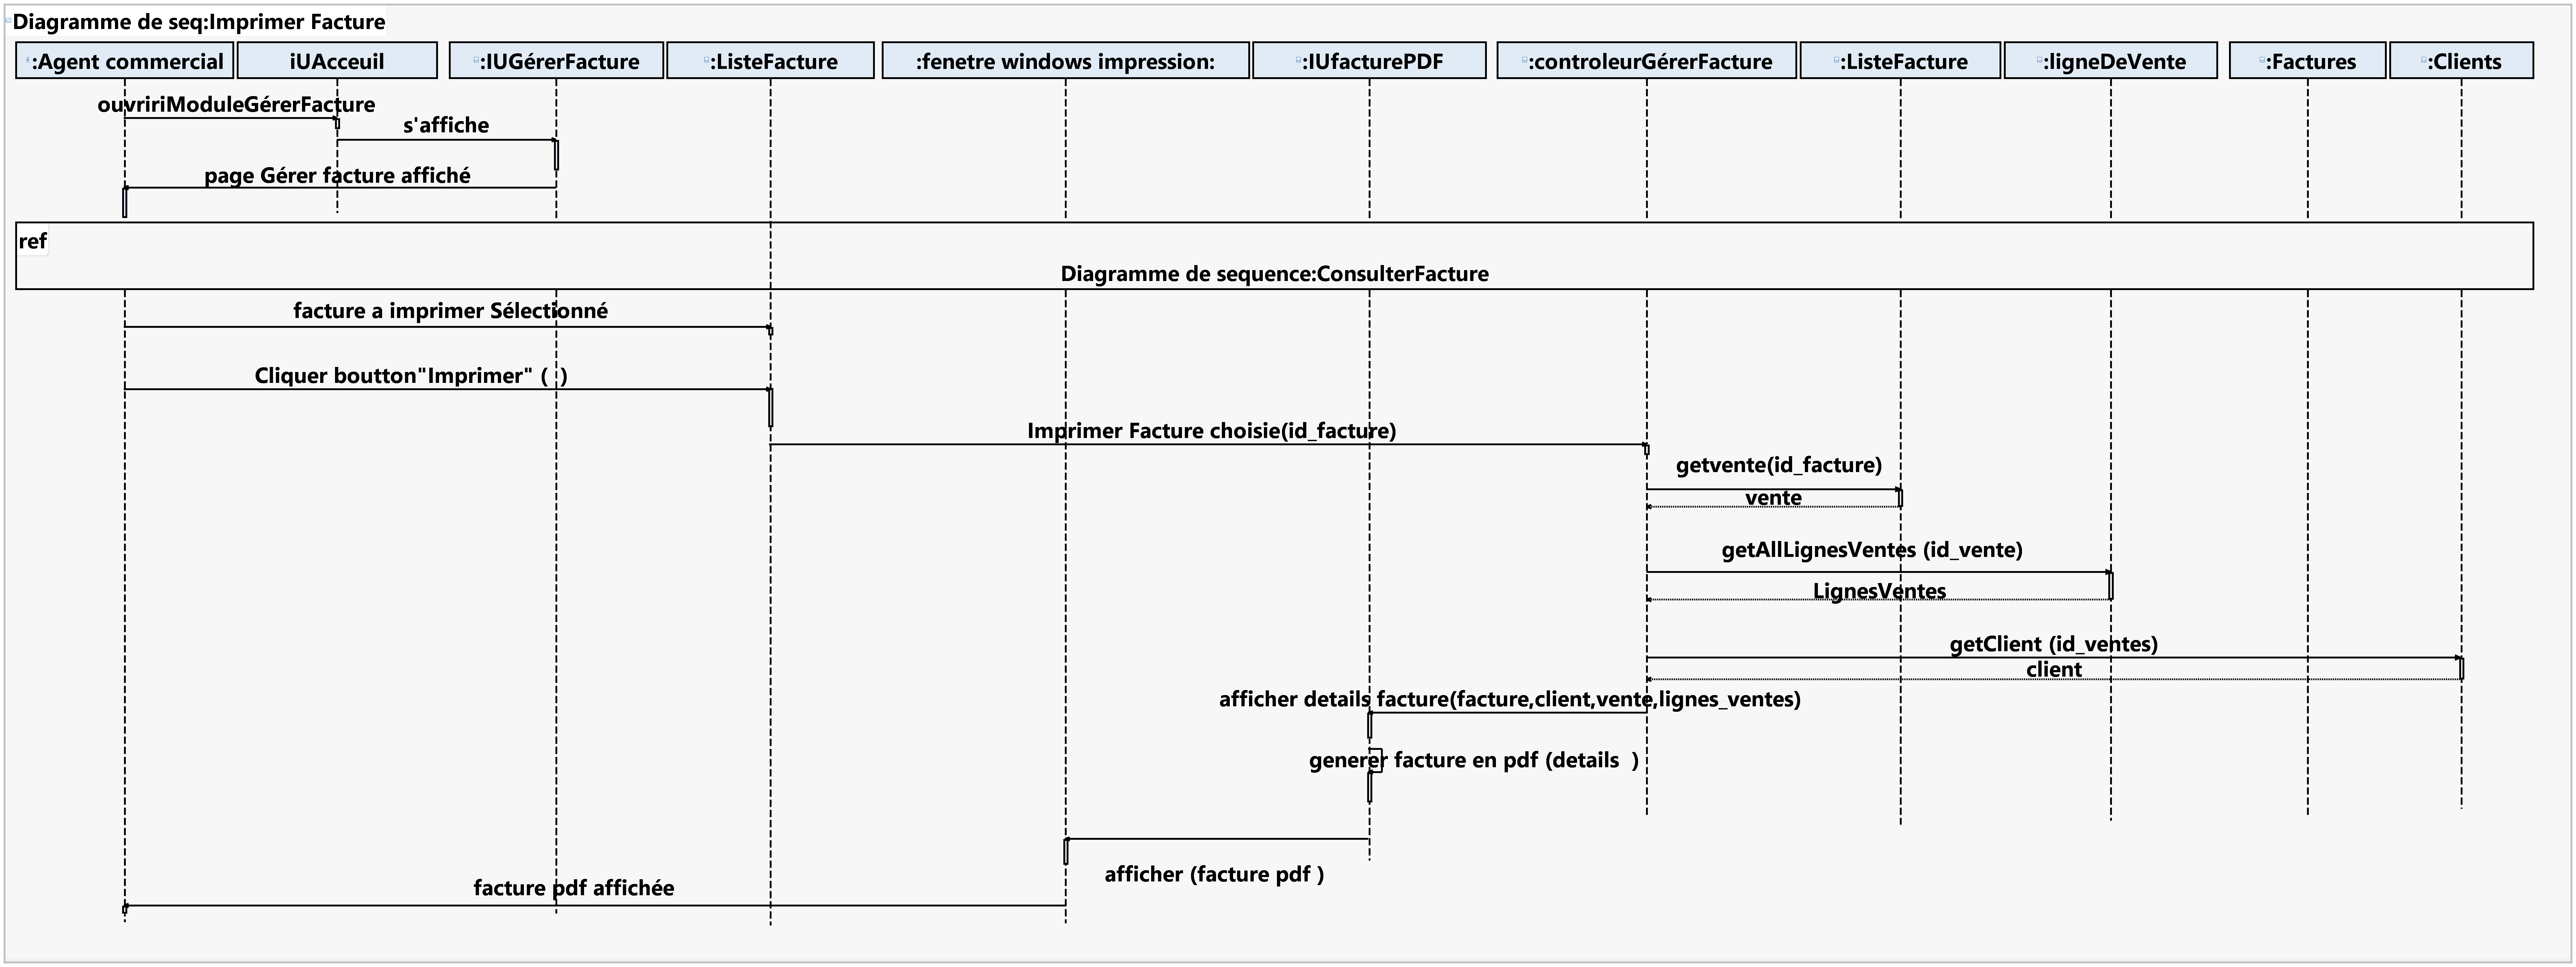
\includegraphics[width=1.15\textwidth, height=0.78\textheight]{images/MC_DiagrammeSéquenceImprimerFacture_1.png}%
  }
  \caption{Diagramme de séquence pour le cas d'utilisation Imprimer Facture}
  \label{fig:seqImprimerFacture}
\end{figure}

\needspace{0.88\textheight}
\subsection{Diagramme de Séquence du Cas D'utilisation Envoyer via WhatsApp}

\begin{figure}[H]
  \centering
  \makebox[\textwidth][c]{%
    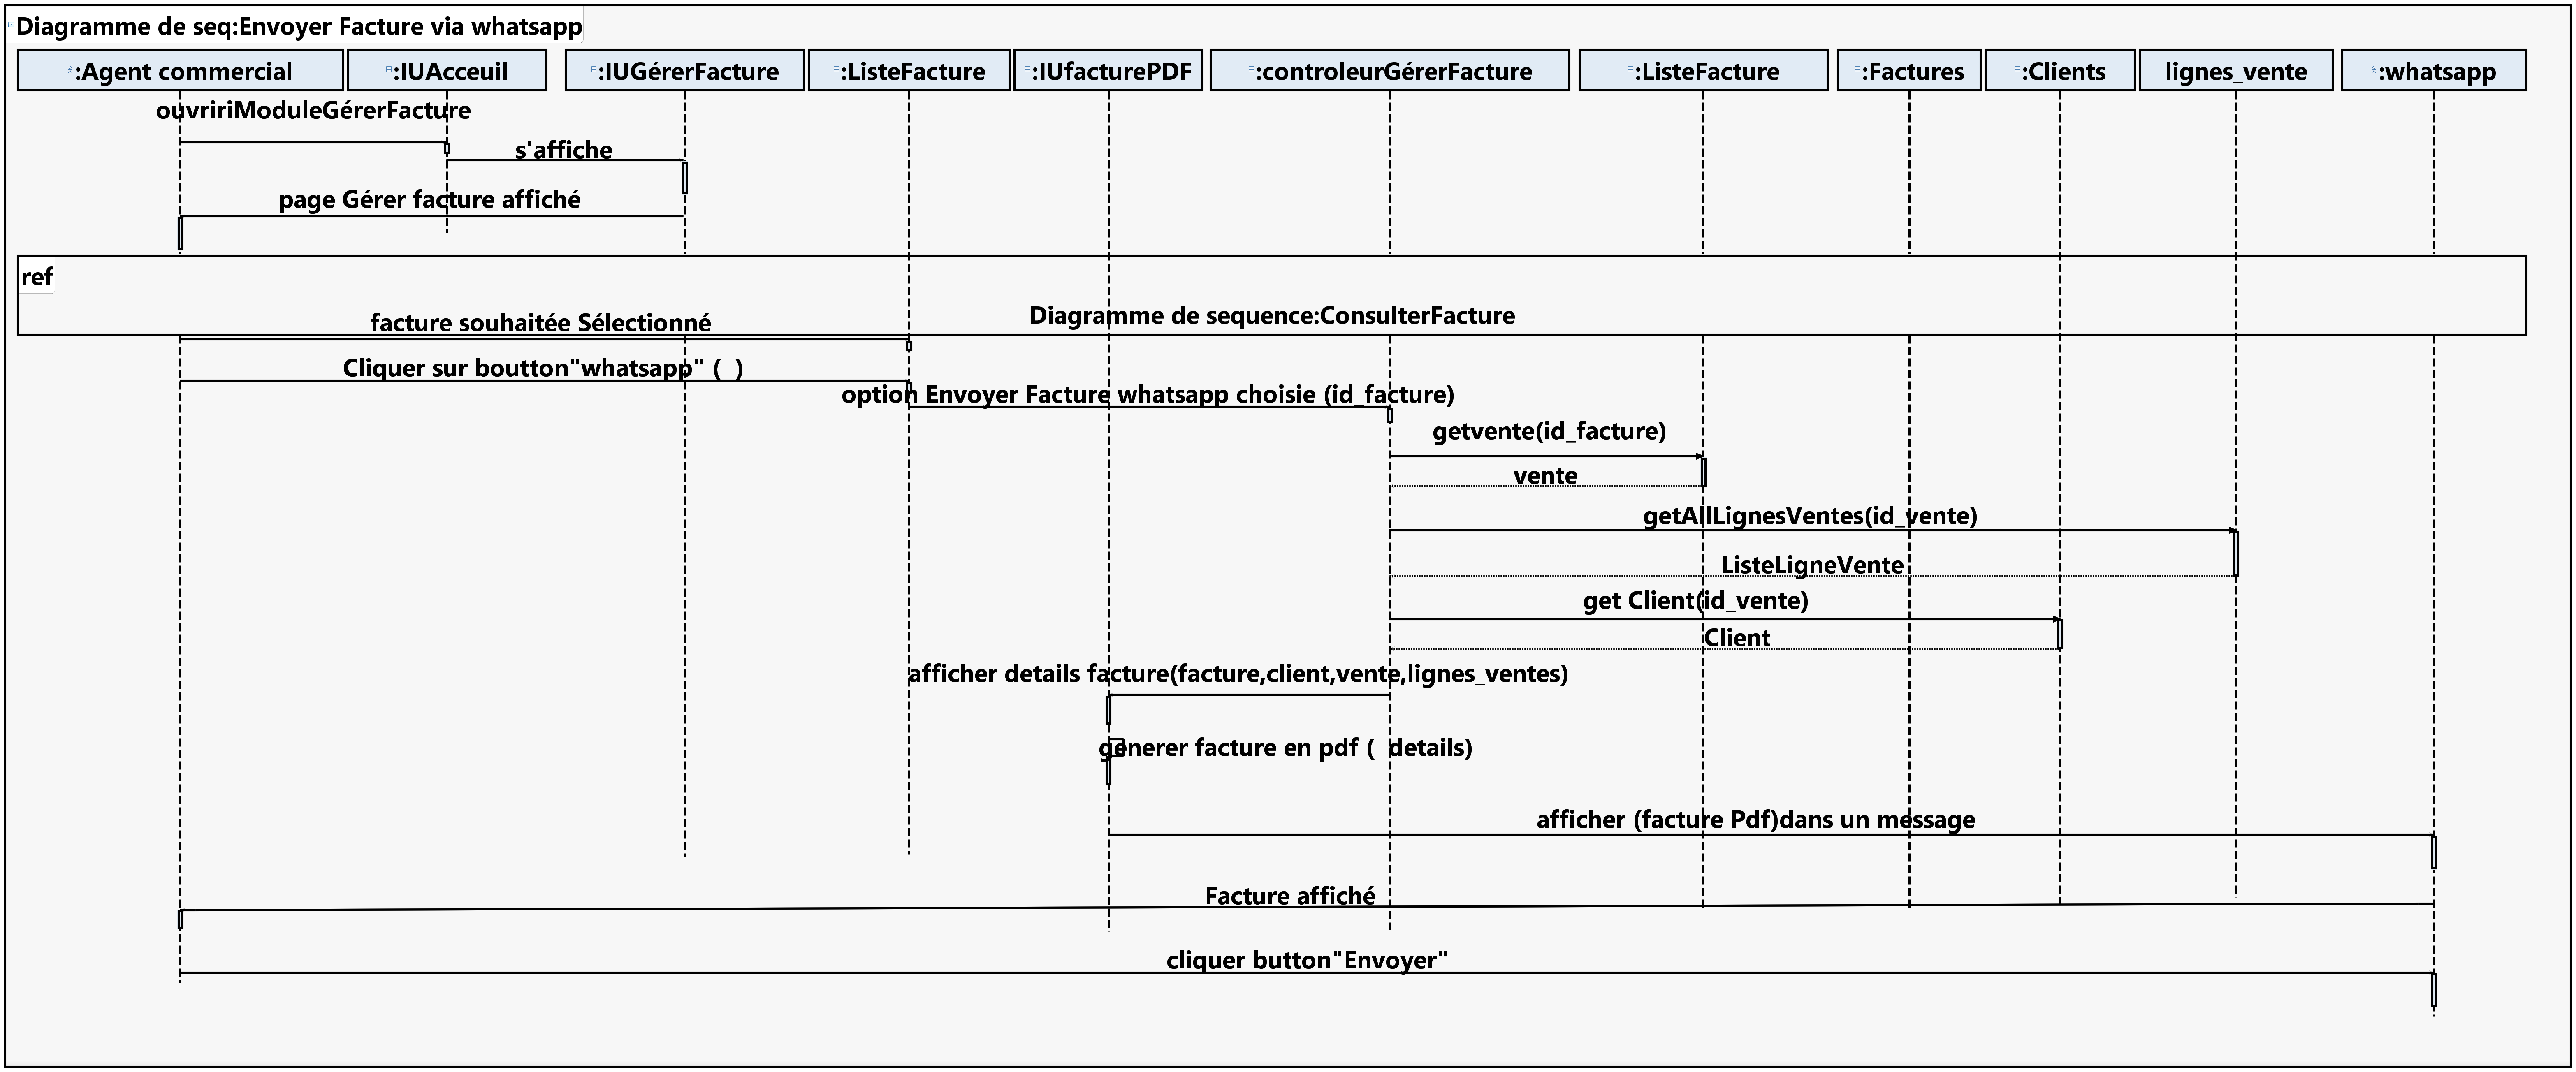
\includegraphics[width=1.15\textwidth, height=0.78\textheight]{images/MC_DiagrammeSéquence1_1.png}%
  }
  \caption{Diagramme de séquence pour le cas d'utilisation Envoyer via WhatsApp}
  \label{fig:seqWhatsApp}
\end{figure}

\needspace{0.88\textheight}
\subsection{Diagramme de Classe du Cas D'utilisation Gérer Factures}

\begin{figure}[H]
  \centering
  \makebox[\textwidth][c]{%
    \includegraphics[width=1.15\textwidth, height=0.78\textheight]{images/MC_DiagrammeClasseGérerFacture_1.png}%
  }
  \caption{Diagramme de classe pour le cas d'utilisation Gérer Factures}
  \label{fig:classeFactures}
\end{figure}
\newpage

\section{Conception du Cas D'utilisation Gérer Notifications}

\needspace{0.88\textheight}
\subsection{Traçabilité MCU/MC pour le Cas D'utilisation Gérer Notifications}

\begin{figure}[H]
  \centering
  \includegraphics[width=\textwidth]{images/image22.png}
  \caption{Traçabilité MCU/MC pour le cas d'utilisation Gérer Notifications}
\end{figure}

Cette traçabilité montre quels sont les objets instances de classe participant à la réalisation du cas d'utilisation Gérer Notifications.

L'acteur et les classes impliquées dans ce diagramme sont les suivants :

\begin{itemize}[leftmargin=2em, topsep=4pt, itemsep=4pt]
  \item \textbf{Agent Commercial :} l'acteur qui initie les opérations de gestion des Notifications
  \item \textbf{IUAccueil :} l'interface principale depuis laquelle l'agent accède à la page de gestion des Notifications
  \item \textbf{:IUListeNotifications :} l'interface qui affiche la liste des notifications et permet à l'agent de les consulter, supprimer et marquer comme lue
  \item \textbf{:controleurGérerNotifications :} le contrôleur qui reçoit les actions de l'interface, traite les requêtes de gestion  des notifications.
  \item \textbf{:Notifications :} l'entité du système qui contient les données et les traitements métier relatives aux notifications
\end{itemize}

Le système génère automatiquement deux types de notifications :

\begin{itemize}[leftmargin=2em, topsep=4pt, itemsep=4pt]
  \item \textbf{Notification de stock :} déclenchée automatiquement après chaque vente enregistrée, lorsque la quantité en stock d'un produit atteint un seuil critique. Elle alerte l'agent commercial afin qu'il prenne les mesures nécessaires pour réapprovisionner.

  \item \textbf{Notification d'échéance de facture :} générée par un \textbf{scheduler} (tâche de fond) qui s'exécute au démarrage du serveur puis toutes les heures. Il vérifie les dates d'échéance de toutes les factures non payées et crée automatiquement une notification pour chaque facture dont l'échéance est dépassée, arrive aujourd'hui ou dans les 3 prochains jours.
\end{itemize}

\needspace{0.88\textheight}
\subsection{Diagramme de Séquence du Cas D'utilisation Consulter Notifications}

\begin{figure}[H]
  \centering
  \makebox[\textwidth][c]{%
    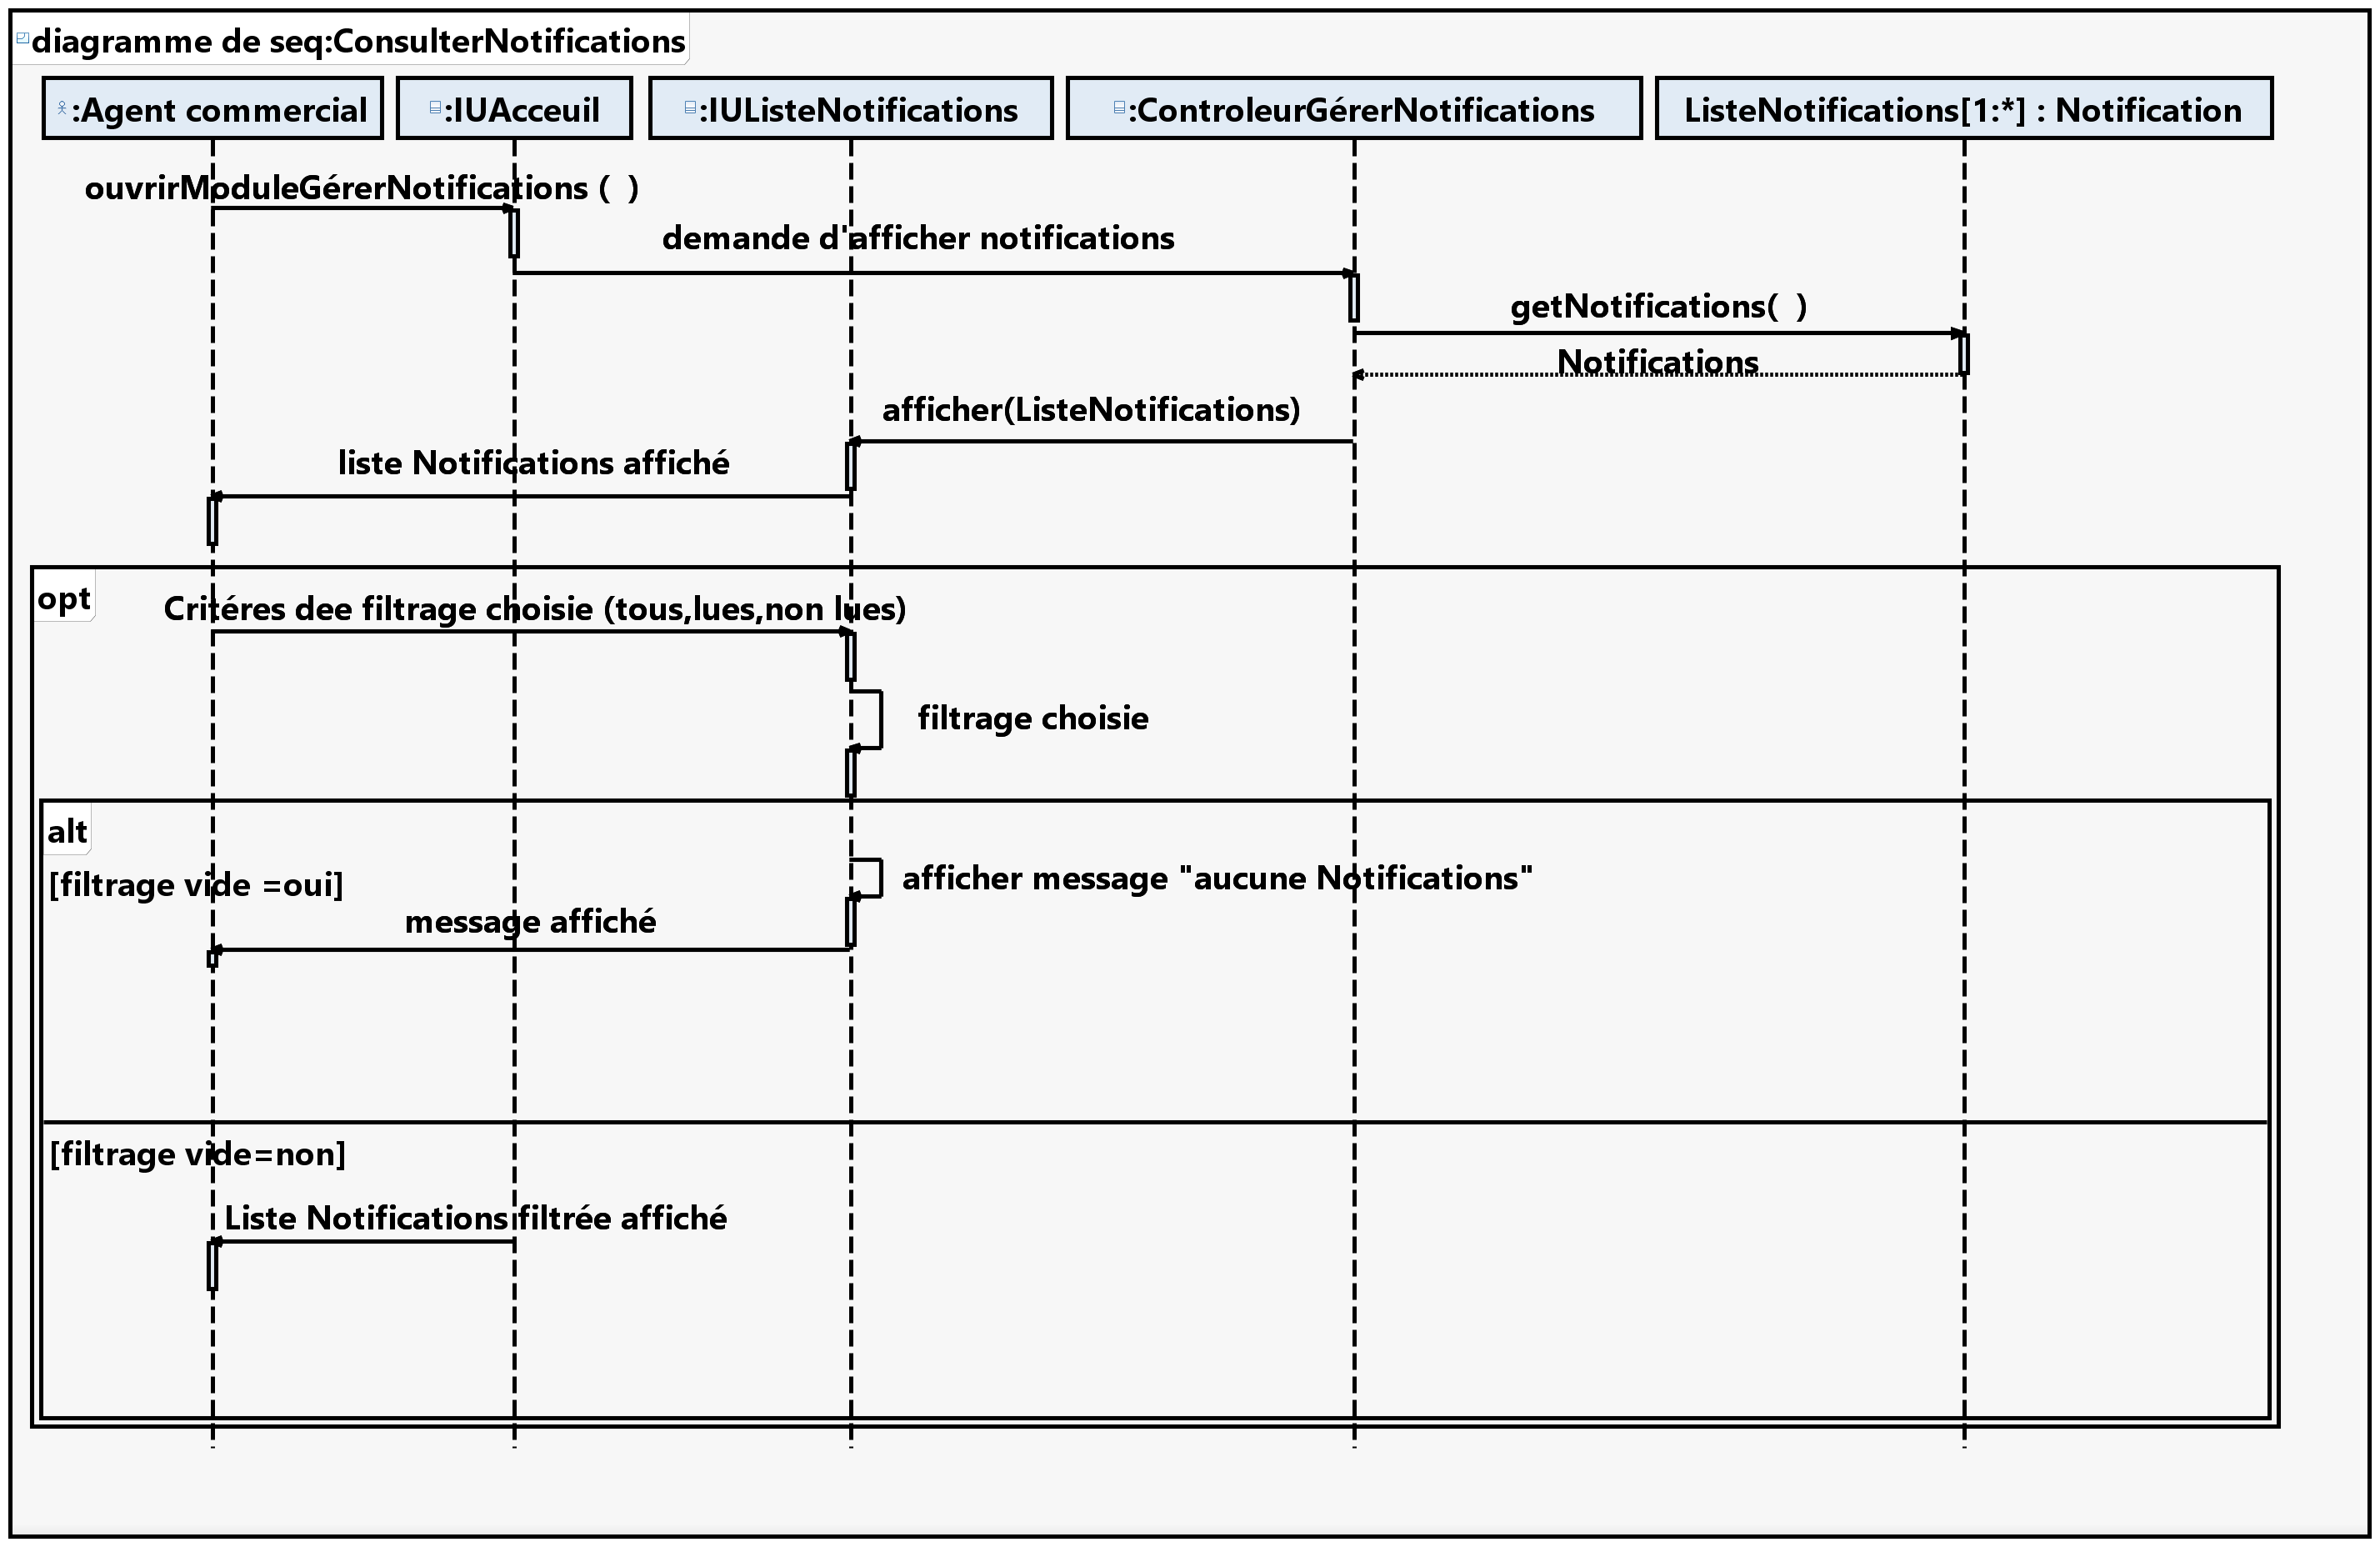
\includegraphics[width=1.15\textwidth, height=0.78\textheight]{images/MC_DiagrammeSéquenceConsulterNotif.png}%
  }
  \caption{Diagramme de séquence pour le cas d'utilisation Consulter Notifications}
  \label{fig:seqConsulterNotif}
\end{figure}

\needspace{0.88\textheight}
\subsection{Diagramme de Séquence du Cas D'utilisation Marquer Notifications Comme Lues}

\begin{figure}[H]
  \centering
  \makebox[\textwidth][c]{%
    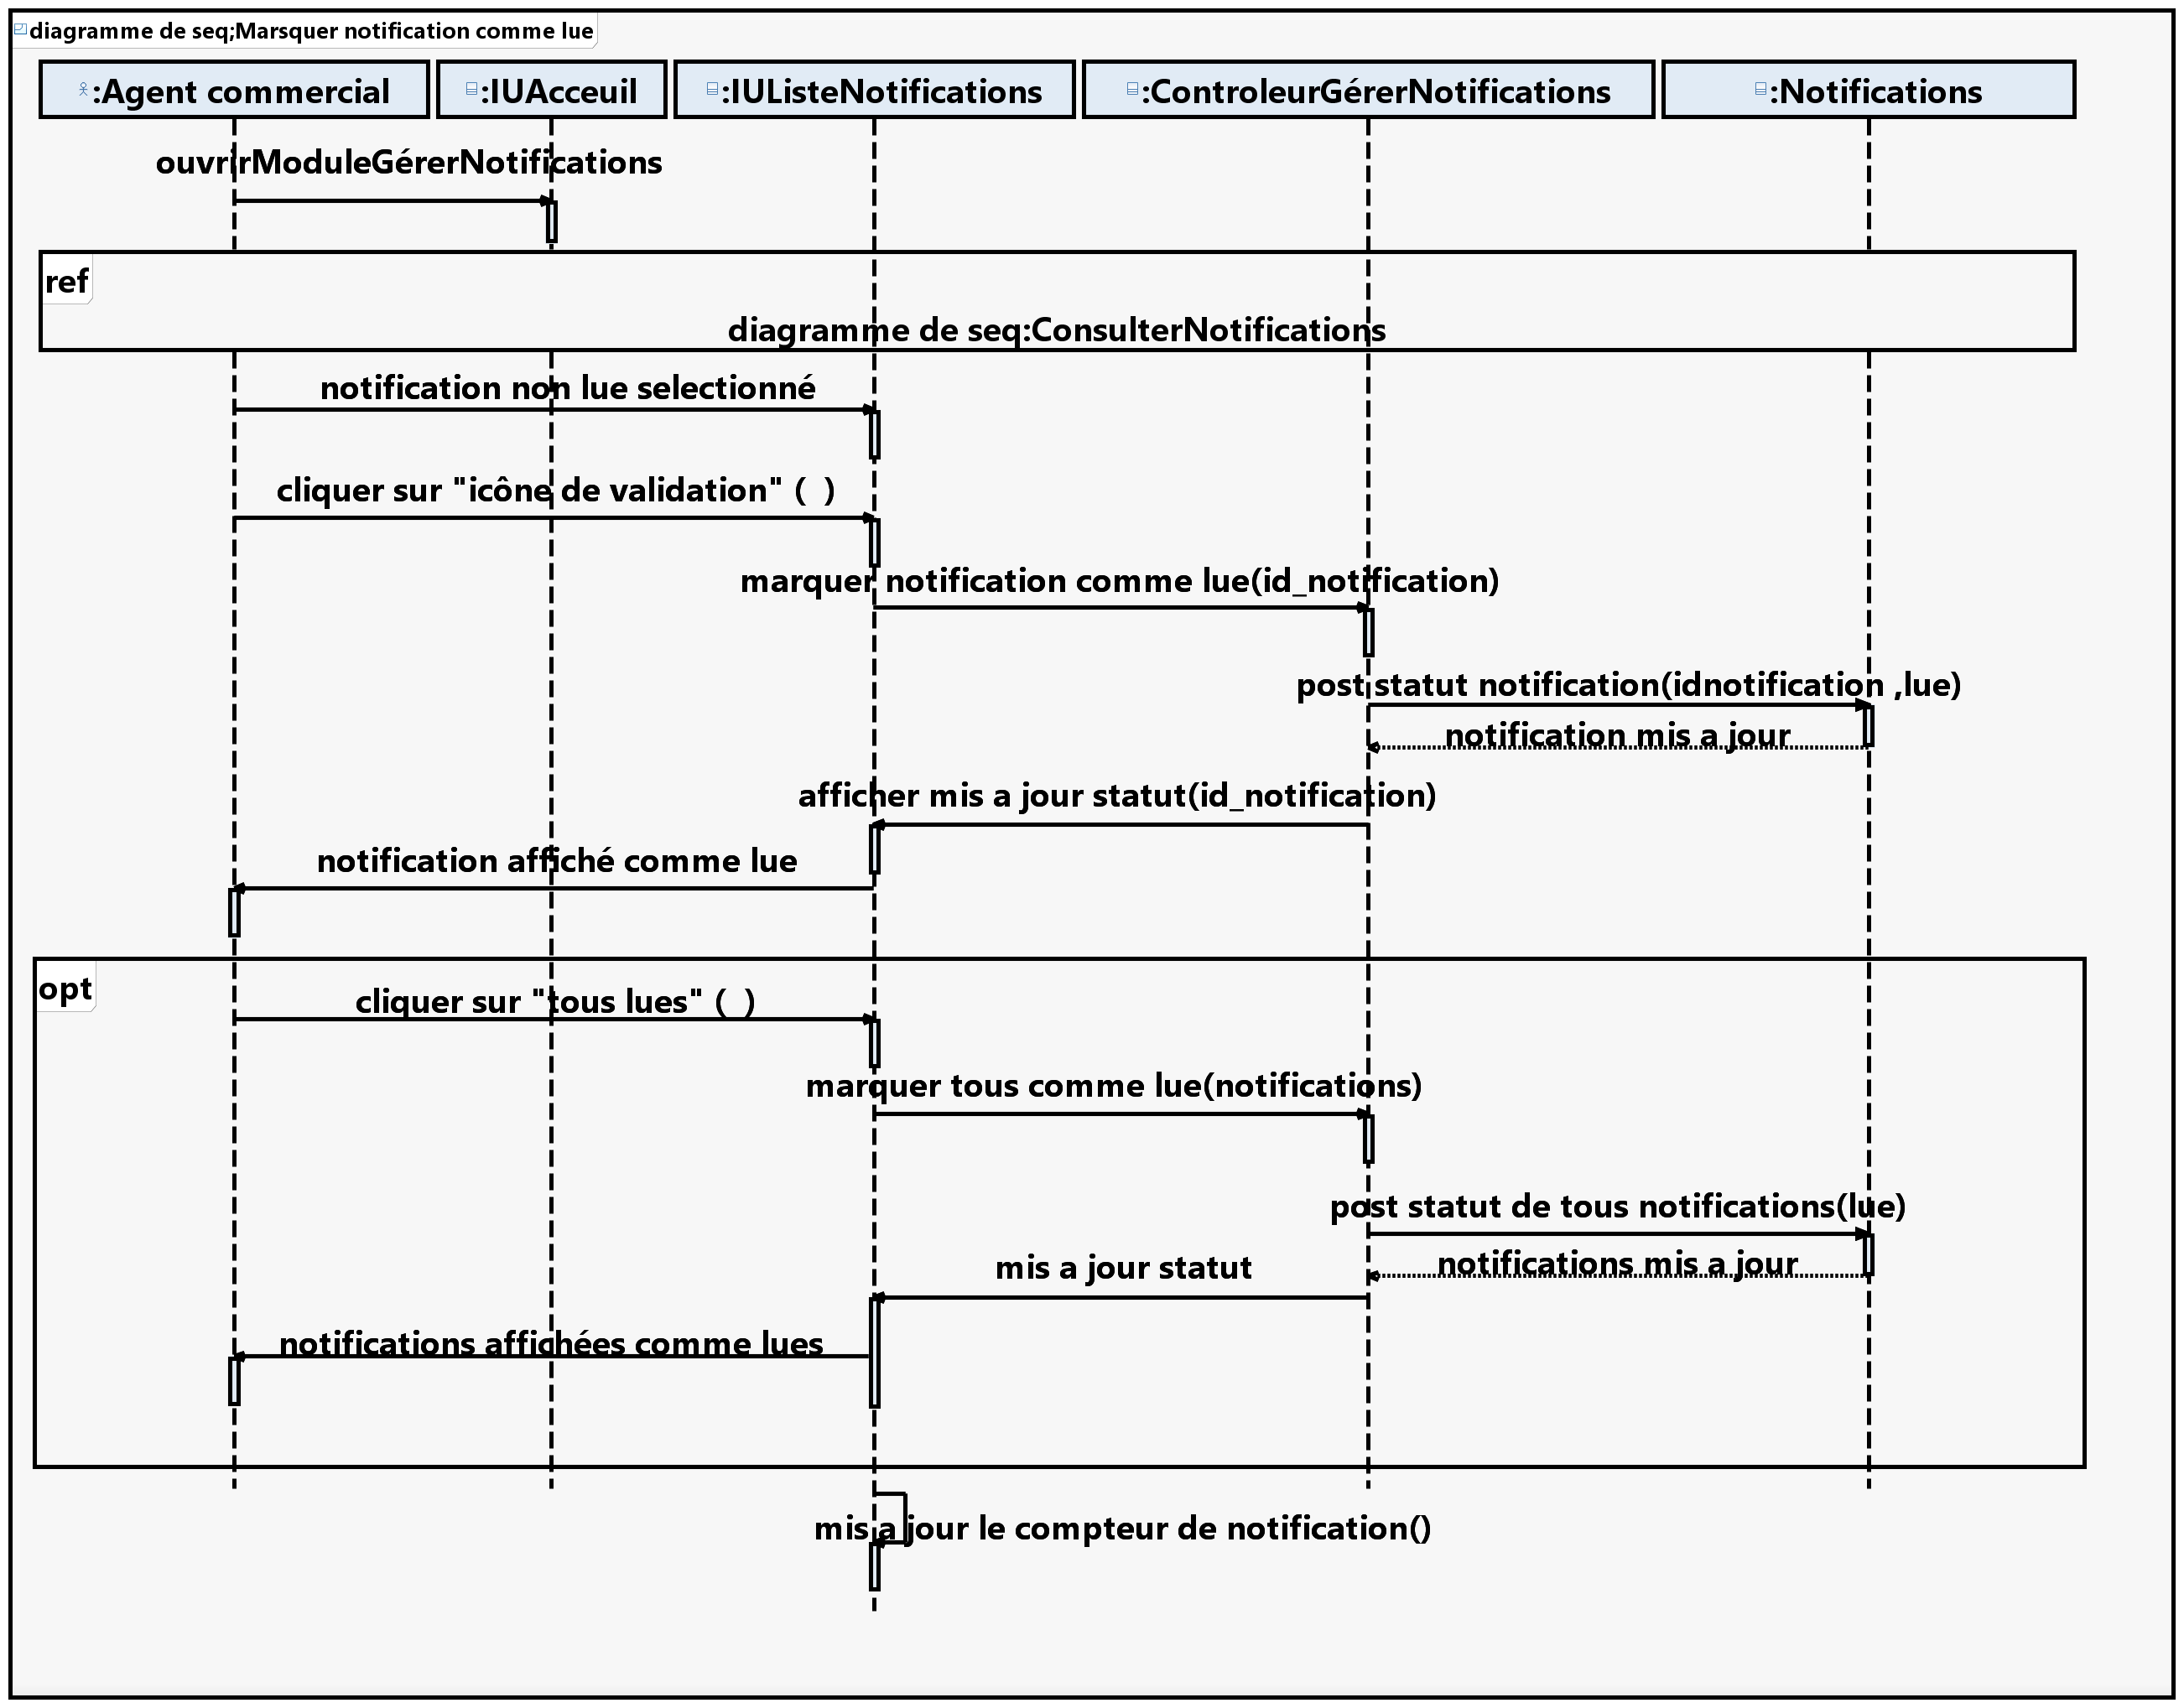
\includegraphics[width=1.15\textwidth, height=0.78\textheight]{images/MC_DiagrammeSéquencemarquercommelue.png}%
  }
  \caption{Diagramme de séquence pour le cas d'utilisation Marquer Notifications Comme Lues}
  \label{fig:seqMarquerLues}
\end{figure}

\needspace{0.88\textheight}
\subsection{Diagramme de Séquence du Cas D'utilisation Supprimer Notifications}

\begin{figure}[H]
  \centering
  \makebox[\textwidth][c]{%
    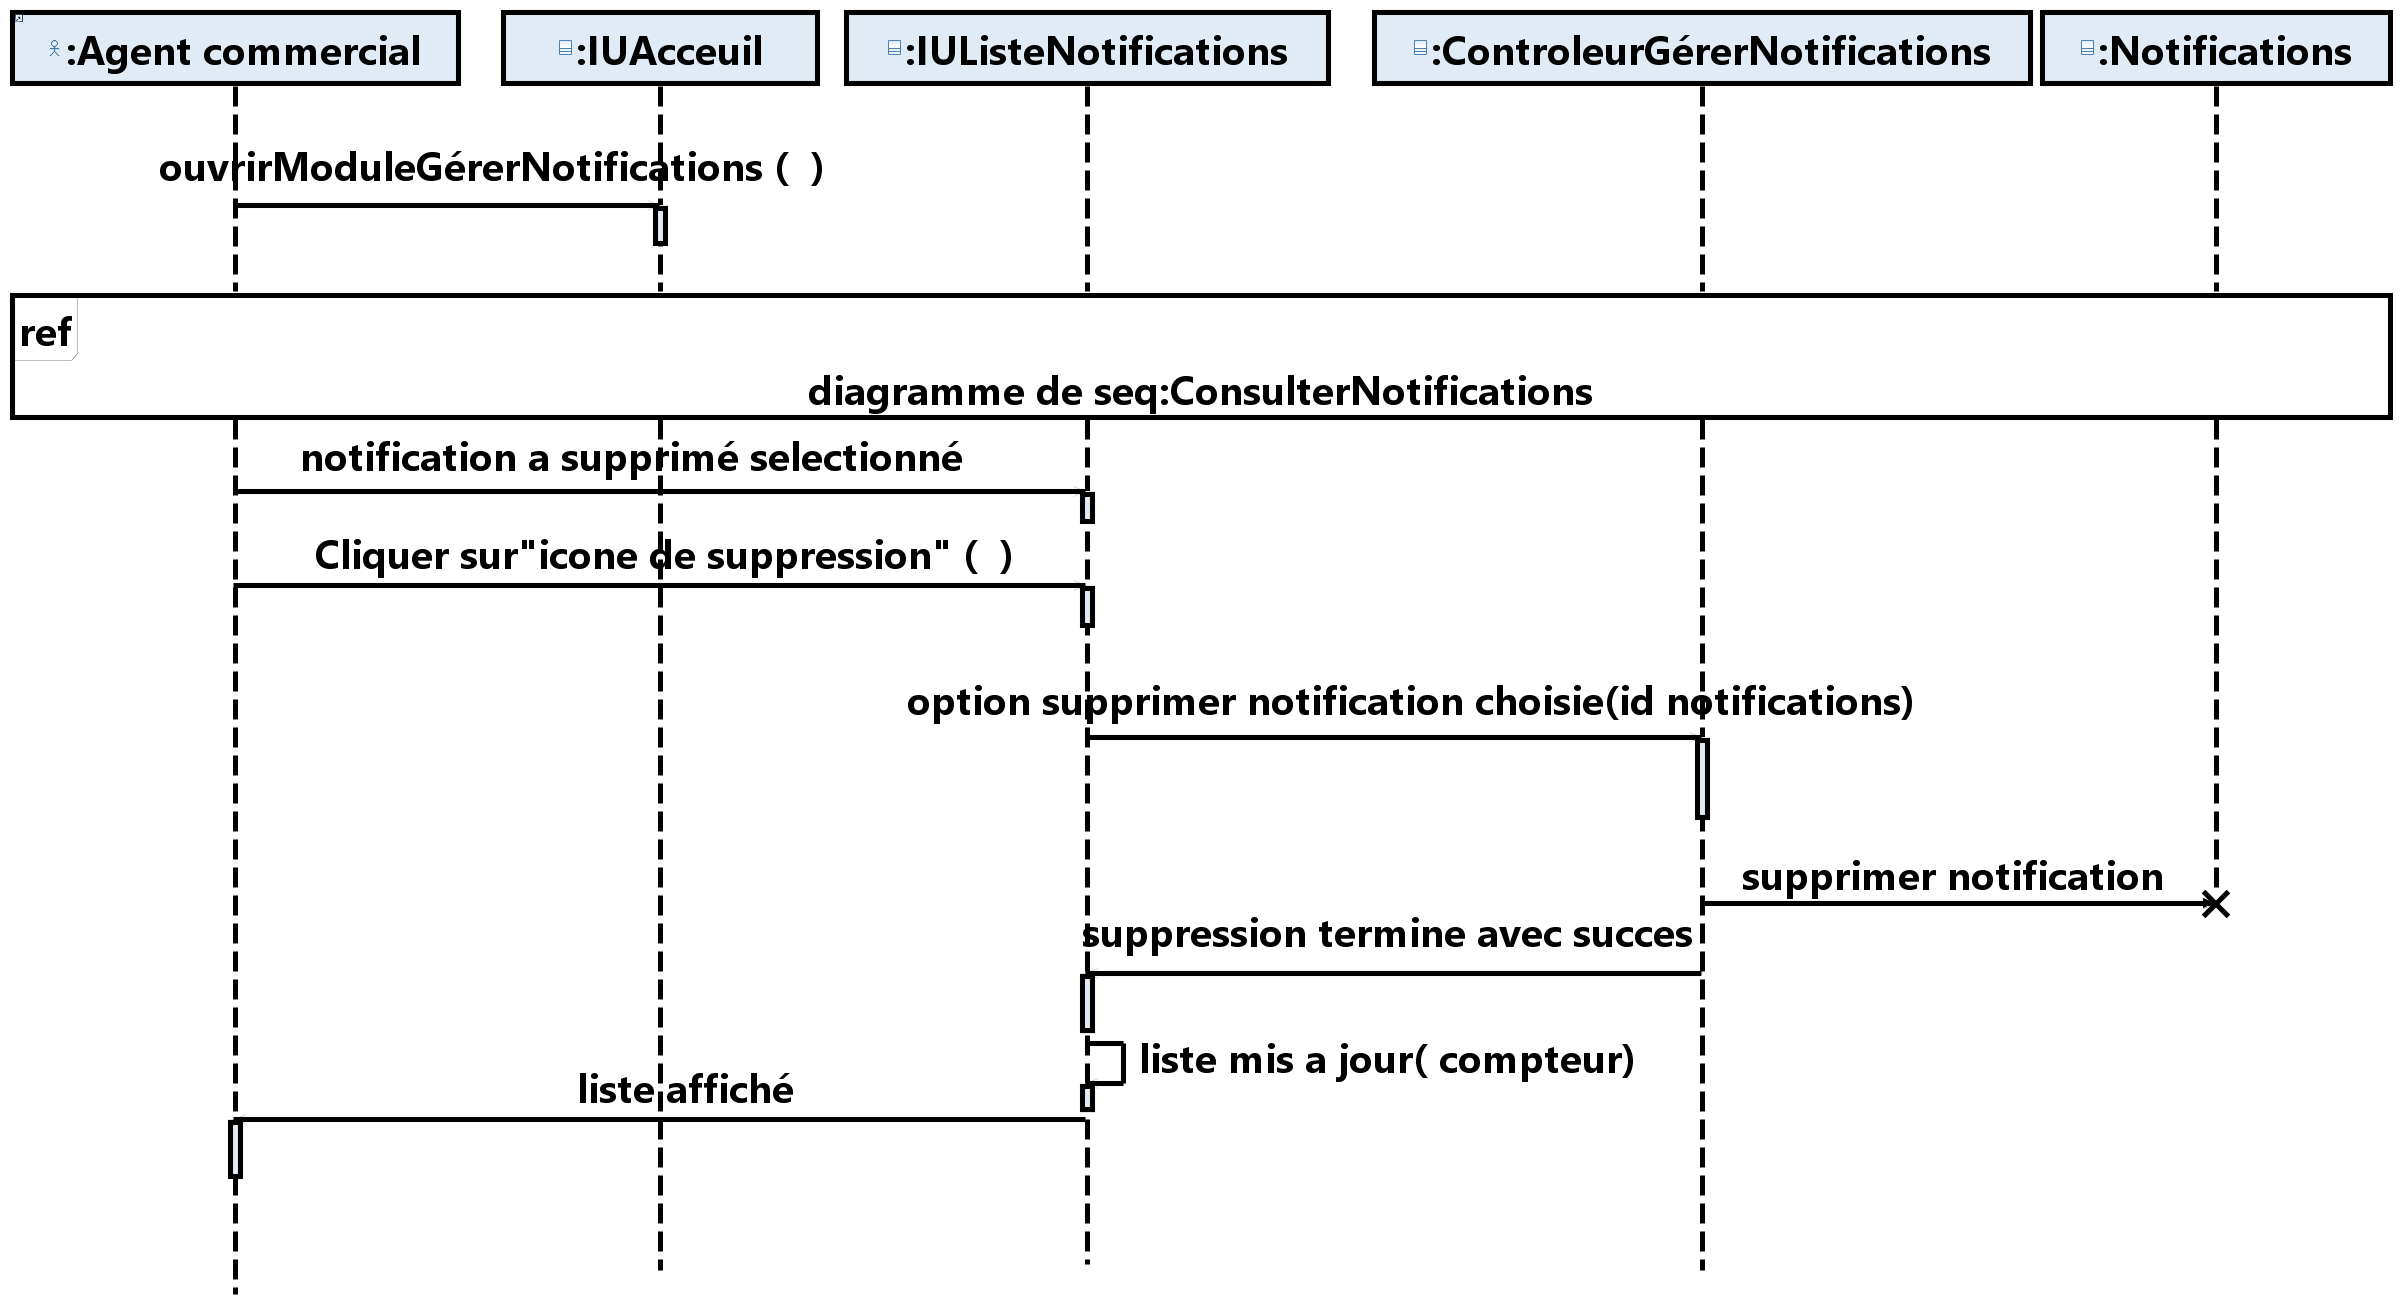
\includegraphics[width=1.15\textwidth, height=0.78\textheight]{images/MC_DiagrammeSéqSupprimerNotifications_1.png}%
  }
  \caption{Diagramme de séquence pour le cas d'utilisation Supprimer Notifications}
  \label{fig:seqSupprimerNotif}
\end{figure}

\needspace{0.88\textheight}
\subsection{Diagramme de Classe du Cas D'utilisation Gérer Notifications}

\begin{figure}[H]
  \centering
  \makebox[\textwidth][c]{%
    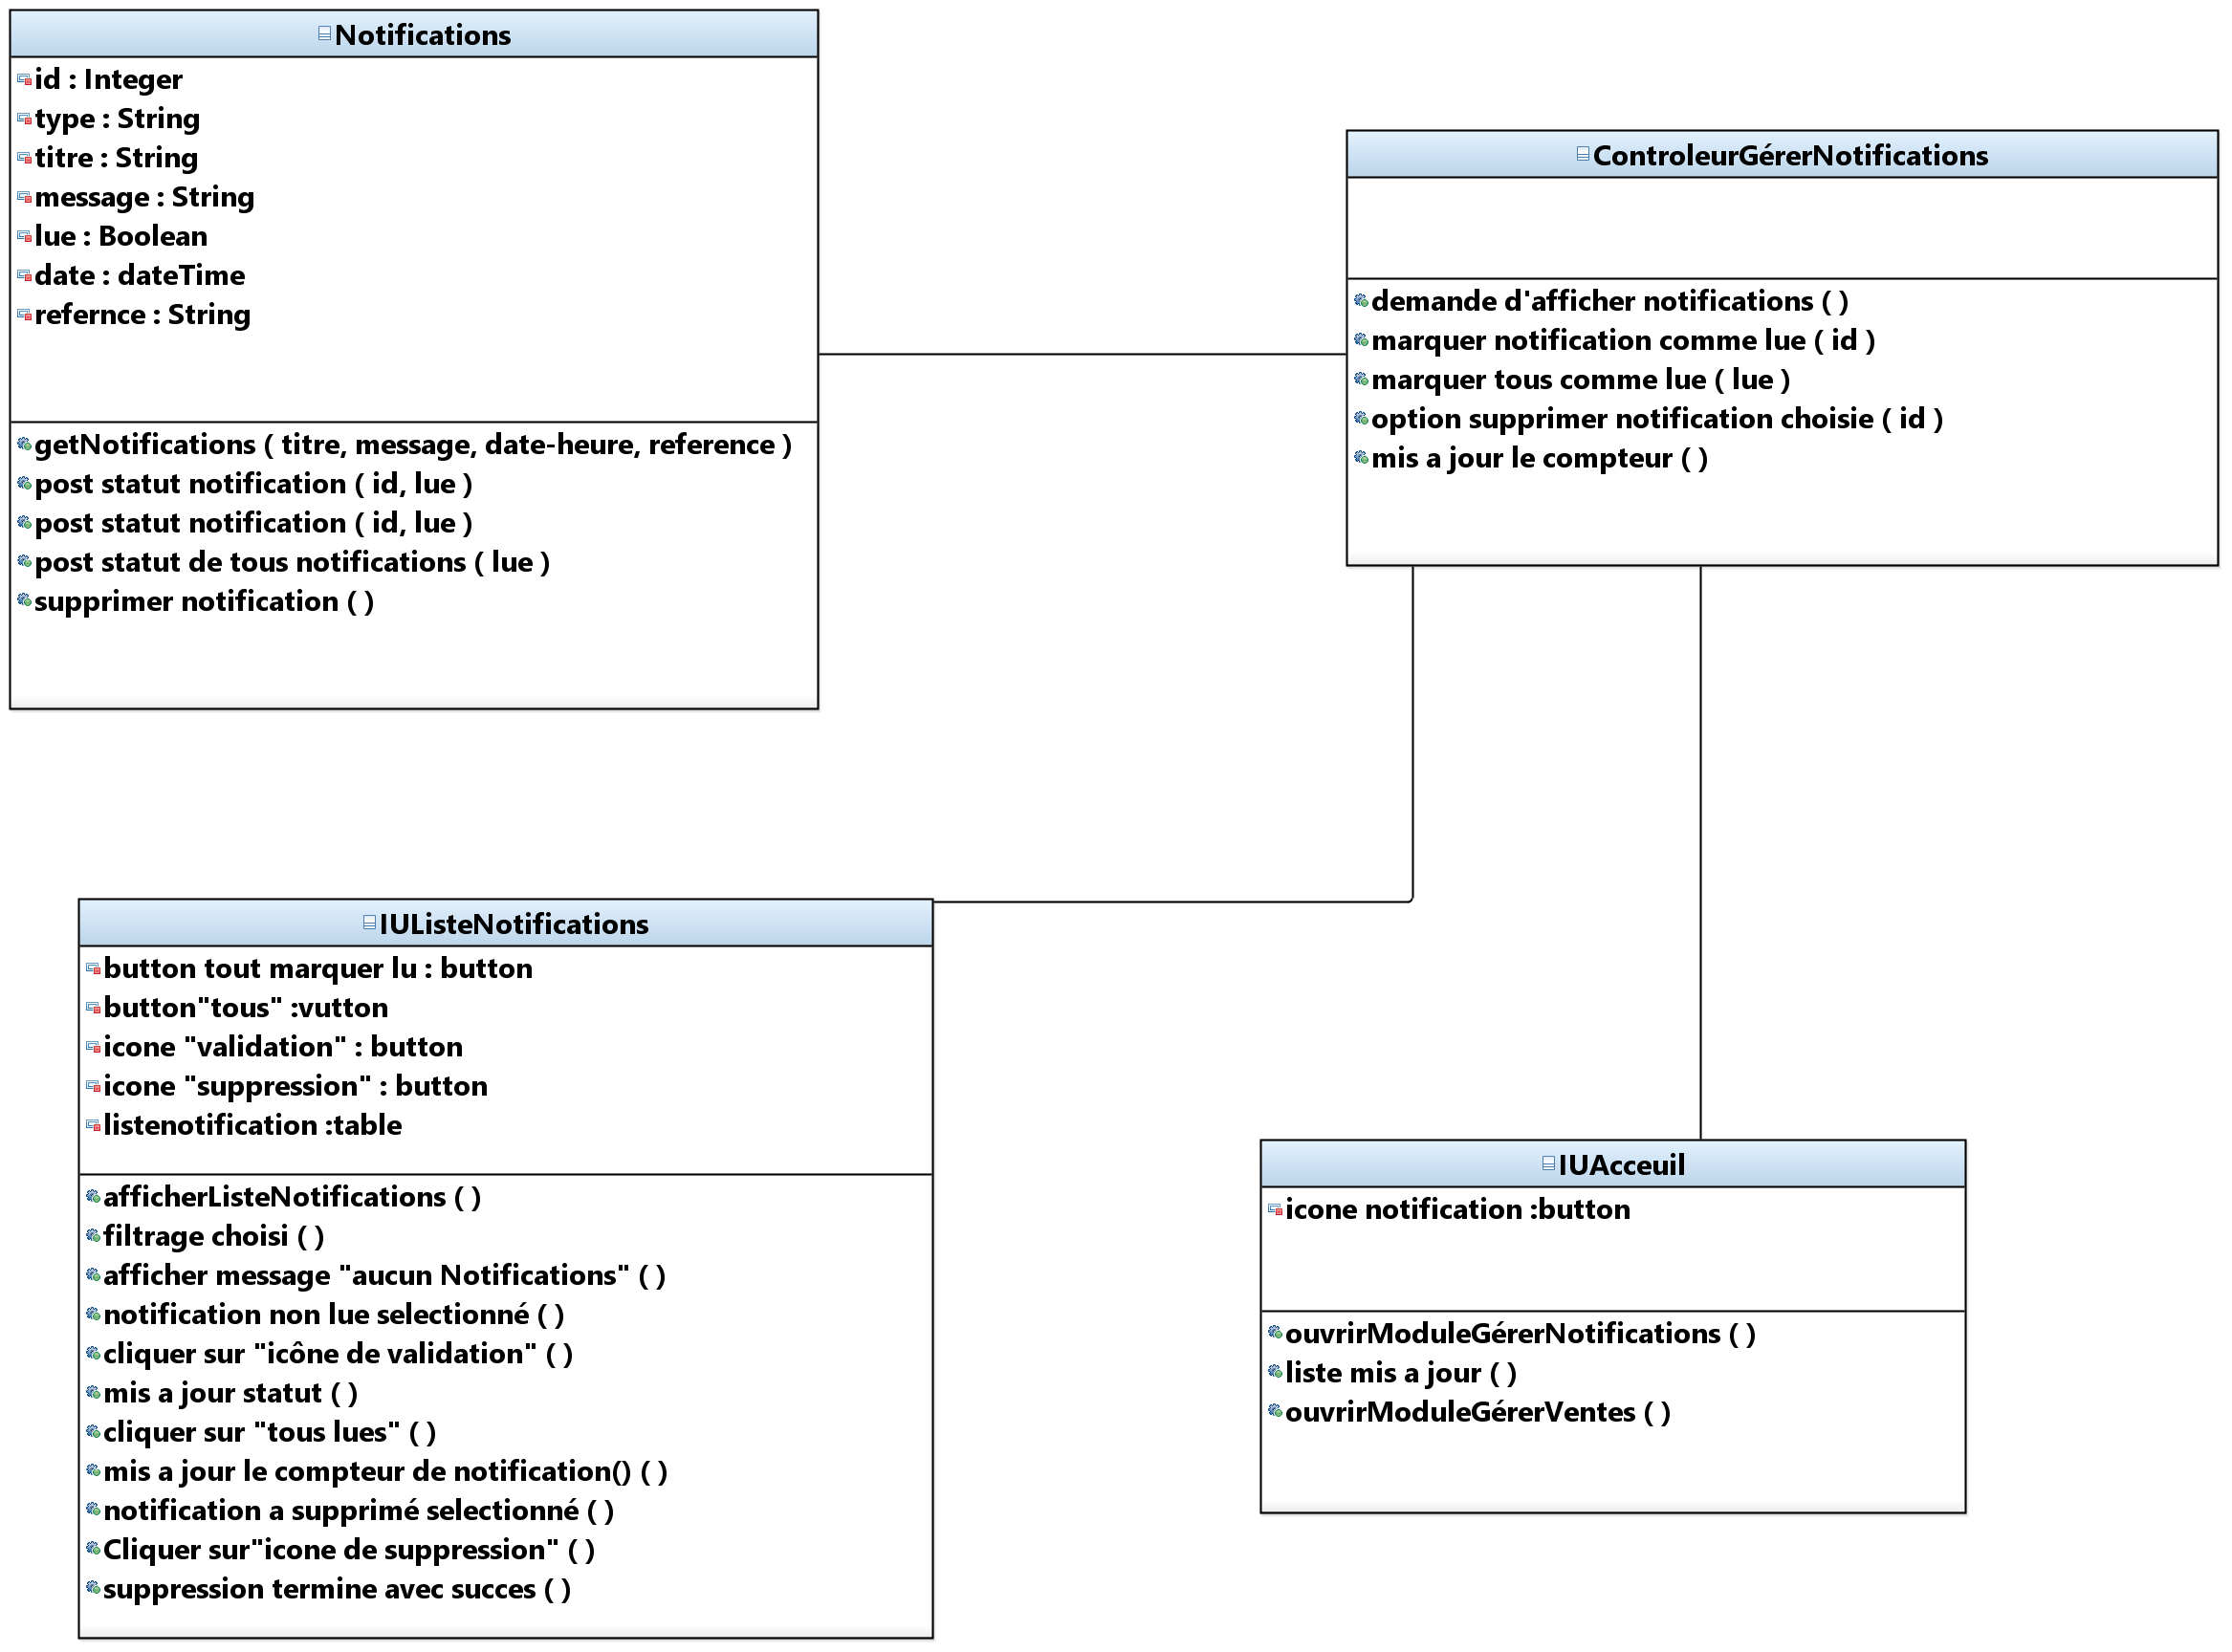
\includegraphics[width=1.05\textwidth, height=0.65\textheight]{images/MC_DiagrammeClasseGérerNotifications.png}%
  }
  \caption{Diagramme de classe pour le cas d'utilisation Gérer Notifications}
  \label{fig:classeNotifications}
\end{figure}
\newpage

\section{Conception des Tableaux de Bord}
\label{sec:ch3:tdb}

\subsection*{Conception de Cas D'utilisation Consulter  Tableaux de Bord}

\begin{figure}[H]
  \centering
  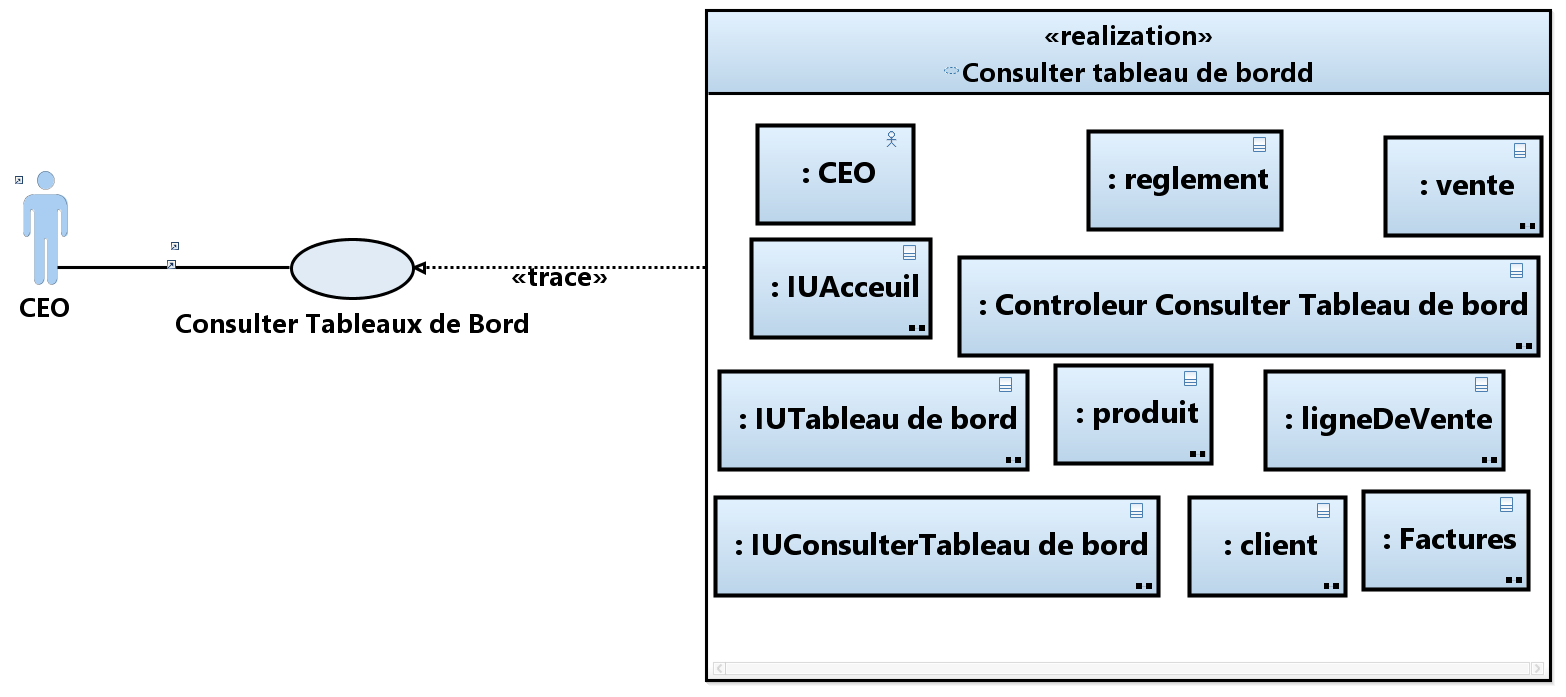
\includegraphics[width=\textwidth]{images/MC_tracabiliteMCUMCConsultertableaudebord_2 (1).png}
  \caption{Traçabilité MCU/MC pour le ca d'utilisation consulter tableaux de bord}
\end{figure}

Cette traçabilité montre quels sont les objets instances de classe participant à la réalisation du cas d'utilisation Consulter Tableaux de Bord.

L'acteur et les classes impliquées dans ce diagramme sont les suivants :

\begin{itemize}[leftmargin=2em, topsep=4pt, itemsep=4pt]
  \item \textbf{CEO :} l'acteur qui initie la consultation des tableaux de bord afin de suivre less indicateurs clés de performances
  \item \textbf{IUAccueil :} l'interface principale depuis laquelle le CEO accède à la page de consultation des tableaux de bord
  \item \textbf{IUConsulterTableauDeBord :} l'interface qui affiche les indicateurs et les  graphiques synthétiques du système,
  \item \textbf{controleur consulterTableaux de bord :} le contrôleur qui reçoit les actions de l'interface, traite les requêtes de consultations et recupére les données apres les calculrer
  \item \textbf{Facture :} l'entité du système qui contient les données et les traitements métier relatives aux factures émises tels que (le montant total,la date de creation,le statut de paiement)
  \item \textbf{Client :} l'entité qui représente le client enregistré dans le systéme utiliser pour calculer les indicateurs tels que (les meilleurs client selon le CA généré,le nombre de vente effectuées par client..)
  \item \textbf{Règlement :} l'entité qui représente les versements total ou partiels effectués sur une facture ,utiliser pour calculer (le montatnt total encaissé,le solde restant du ..)
  \item \textbf{LigneDeVente :} l'entité du système qui contient les données et les traitements métier relatives aux produits liés à une vente,avec sa quantité,son prix de vente et son sous total ,utiliser pour calculer le CA par produitet la marge brute
  \item \textbf{Produit :} l'entité du système qui contient la structure de données et les traitements relative aux produits,utiliser pour nomer et regrouper les lignes de vente par produit ou par catégorie
  \item \textbf{Vente :} l'entité associée à la vente représentant la vente d'origine,utiliser pour calculer les indicateurs d'évolution du CA
\end{itemize}

\clearpage
\subsection{Diagramme de Séquence du Cas D'utilisation Consulter Tableaux de Bord}
\begin{figure}[H]
  \centering
  \makebox[\textwidth][c]{%
    \includegraphics[width=1.15\textwidth, height=0.78\textheight]{images/MC_DiagrammeSéquenceConsulterTableauxdebord.png}%
  }
  \caption{Diagramme de séquence pour le cas d'utilisation Consulter Tableaux de Bord}
  \label{fig:ConsulterTableauxdeBord}
\end{figure}
\clearpage

\subsection{Diagramme de Classe du Cas D'utilisation Consulter Tableaux de Bord}

\begin{figure}[H]
  \centering
  \makebox[\textwidth][c]{%
    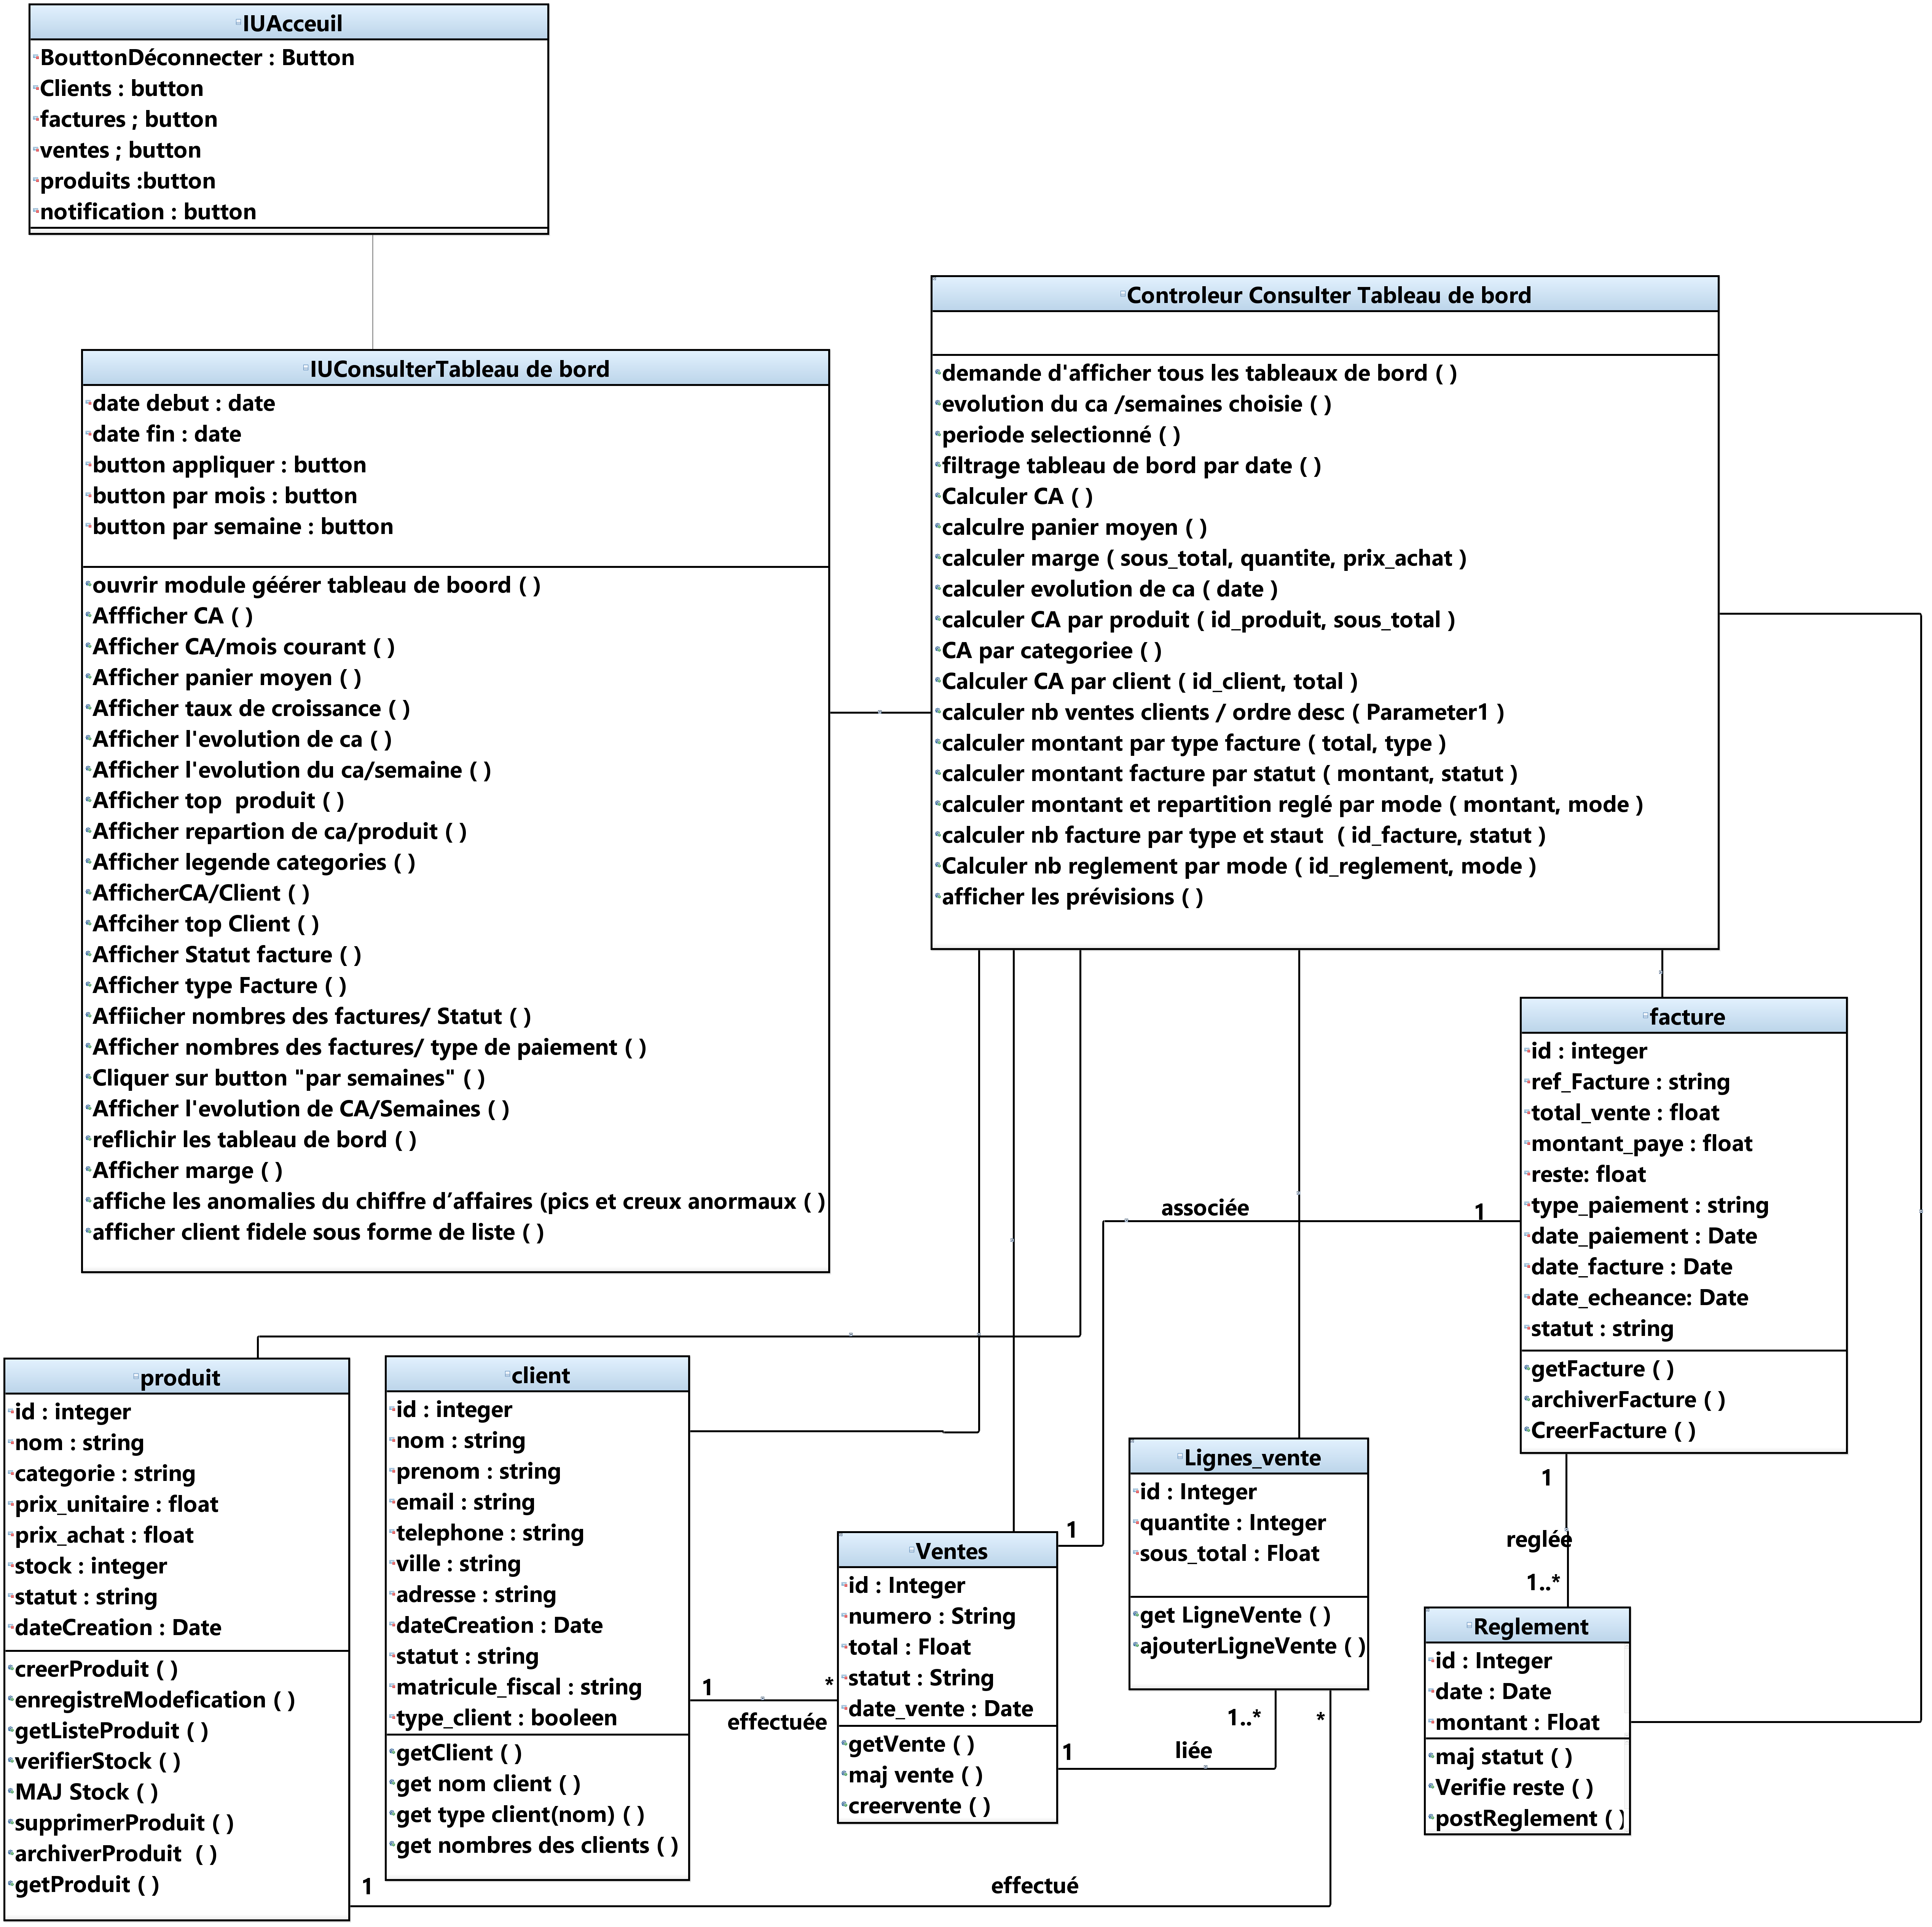
\includegraphics[width=1.05\textwidth, height=0.65\textheight]{images/MC_DiagrammeClasseConsulterTbaleaudebord_1.png}%
  }
  \caption{Diagramme de classe pour le cas d'utilisation Consulter Tableaux de Bord}
  \label{fig:classetableauxdeBord}
\end{figure}

\newpage

%----------------------------------
\section{Processus ETL}
%----------------------------------

Afin d'assurer une migration fluide et fiable des données historiques du client 
vers notre nouveau système, nous avons mis en place un processus ETL structuré 
en trois phases distinctes.

L'ETL (Extract, Transform, Load) est un processus d'intégration de données qui 
combine des données provenant de l'ancien système Odoo utilisé par le client et 
destiné à être remplacé par la solution développée dans le cadre de ce projet, 
exportées sous format CSV, en un ensemble de données unifié, cohérent et adapté 
à notre nouveau système. Ce processus consiste à extraire des données brutes à 
partir des fichiers CSV contenant les informations sur les clients, les produits, 
les ventes et les factures, à les transformer afin de les nettoyer pour répondre 
à des exigences spécifiques, puis à les charger dans un entrepôt de données. 
Il en résulte un référentiel centralisé de données structurées et de haute qualité, 
prêt à être analysées et visualisées dans les tableaux de bord décisionnel 
\cite{etl_ovh}.

\begin{figure}[H]
  \centering
  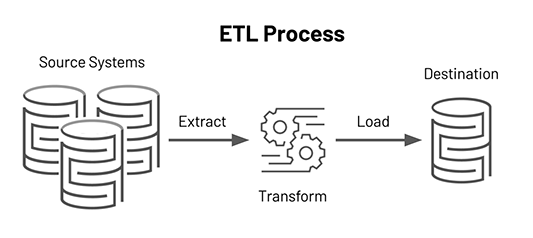
\includegraphics[width=0.75\textwidth]{images/etl.png}
  \caption{Schéma du processus ETL}
  \label{fig:etl-process}
\end{figure}

\subsection{Extraction}

La phase d'extraction dans notre système est conçue pour lire les données brutes 
issues des fichiers CSV exportés depuis l'ancien système (Odoo), représentant 
l'historique de la société. Cette extraction n'effectue aucune modification sur 
les données sources ; elle garantit la préservation de leur état original ainsi 
que l'intégrité de la migration.

\subsection{Transformation}

La phase de transformation dans notre système consiste à appliquer des règles de 
nettoyage et de conformité nécessaires à l'intégration des données. Ce processus 
implique le filtrage des données non pertinentes, la normalisation des dates et 
des formats, ainsi que la séparation des champs.

\subsection{Chargement}

La phase de chargement consiste à charger les données transformées dans la base 
de données de notre système. Ces données, désormais organisées, nettoyées et 
conformes à la structure des tables actuelles, sont prêtes à être exploitées 
pour l'analyse et le reporting.

\clearpage
\subsection*{Conception de Cas D'utilisation Consulter Prévisions}

\begin{figure}[H]
  \centering
  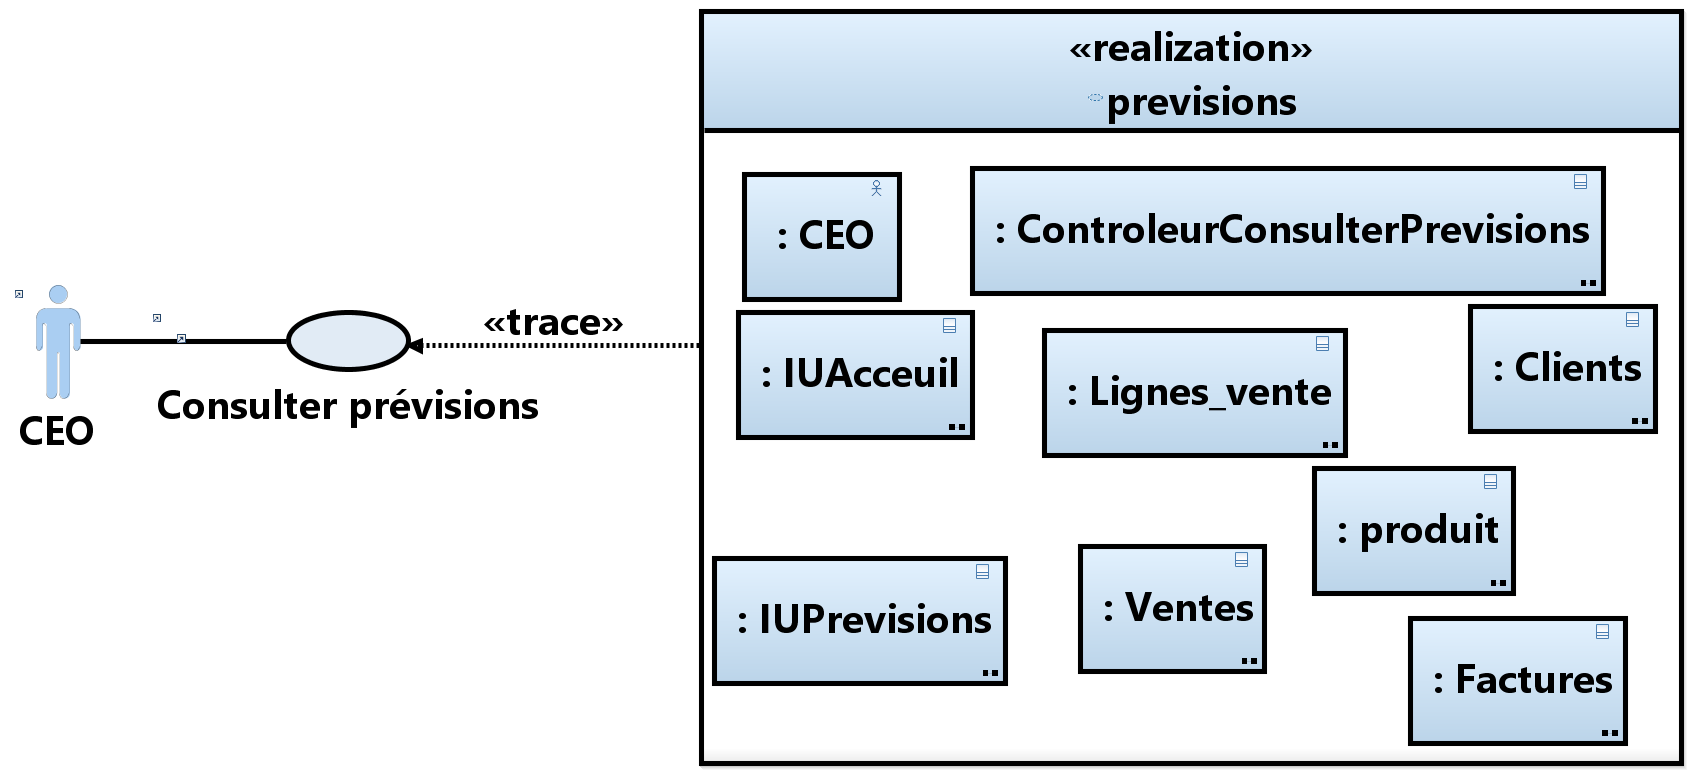
\includegraphics[width=\textwidth]{images/MC_tracabilitéMCUMCConsulterPrevision.png}
  \caption{Traçabilité MCU/MC pour le cas d'utilisation Consulter Prévisions}
\end{figure}

Cette traçabilité montre quels sont les objets instances de classe participant à la réalisation du cas d'utilisation  Consulter Prévisions

L'acteur et les classes impliquées dans ce diagramme sont les suivants :

\begin{itemize}[leftmargin=2em, topsep=4pt, itemsep=4pt]
  \item \textbf{CEO :} l'acteur qui initie la consultation des
  \item \textbf{IUAccueil :} l'interface principale depuis laquelle l'agent accède à la page de gestion des
  \item \textbf{IU Prévisions :} l'interface qui affiche les résultats des prévisions sous forme de graphiques et d'indicateurs synthétiques
  \item \textbf{controleur Consulter prévisions :} le contrôleur qui reçoit les actions de l'interface , applique les algorithmes de prévision et retourne les projections calculées à l'interface pour affichage.
  \item \textbf{Facture :} utilisée pour analyser les historiques de facturation et d'encaissement, afin de prévoir les flux de trésorerie futurs et estimer le taux de recouvrement attendu sur les périodes à venir.
  \item \textbf{Client :} l'entité utilisée pour segmenter les prévisions par client, identifier les clients à potentiel élevé et anticiper l'évolution du chiffre d'affaires généré par chaque client sur les périodes futures.
  \item \textbf{LigneDeVente :} l'entité du système qui contient les données et les traitements métier relatives aux produits liés à une ventepour calculer les tendances de vente par produit et alimenter les modèles de prévision.
  \item \textbf{Produit :} l'entité du système qui contient la structure de données et les traitements relative aux produits, utiliser pour identifier les produits les plus performants et prévoir leur évolution future et projeter l'évolution future du volume et du chiffre d'affaires
\end{itemize}

\needspace{0.88\textheight}
\subsection{Diagramme de Séquence du Cas D'utilisation Consulter Prévisions}

\begin{figure}[H]
  \centering
  \makebox[\textwidth][c]{%
    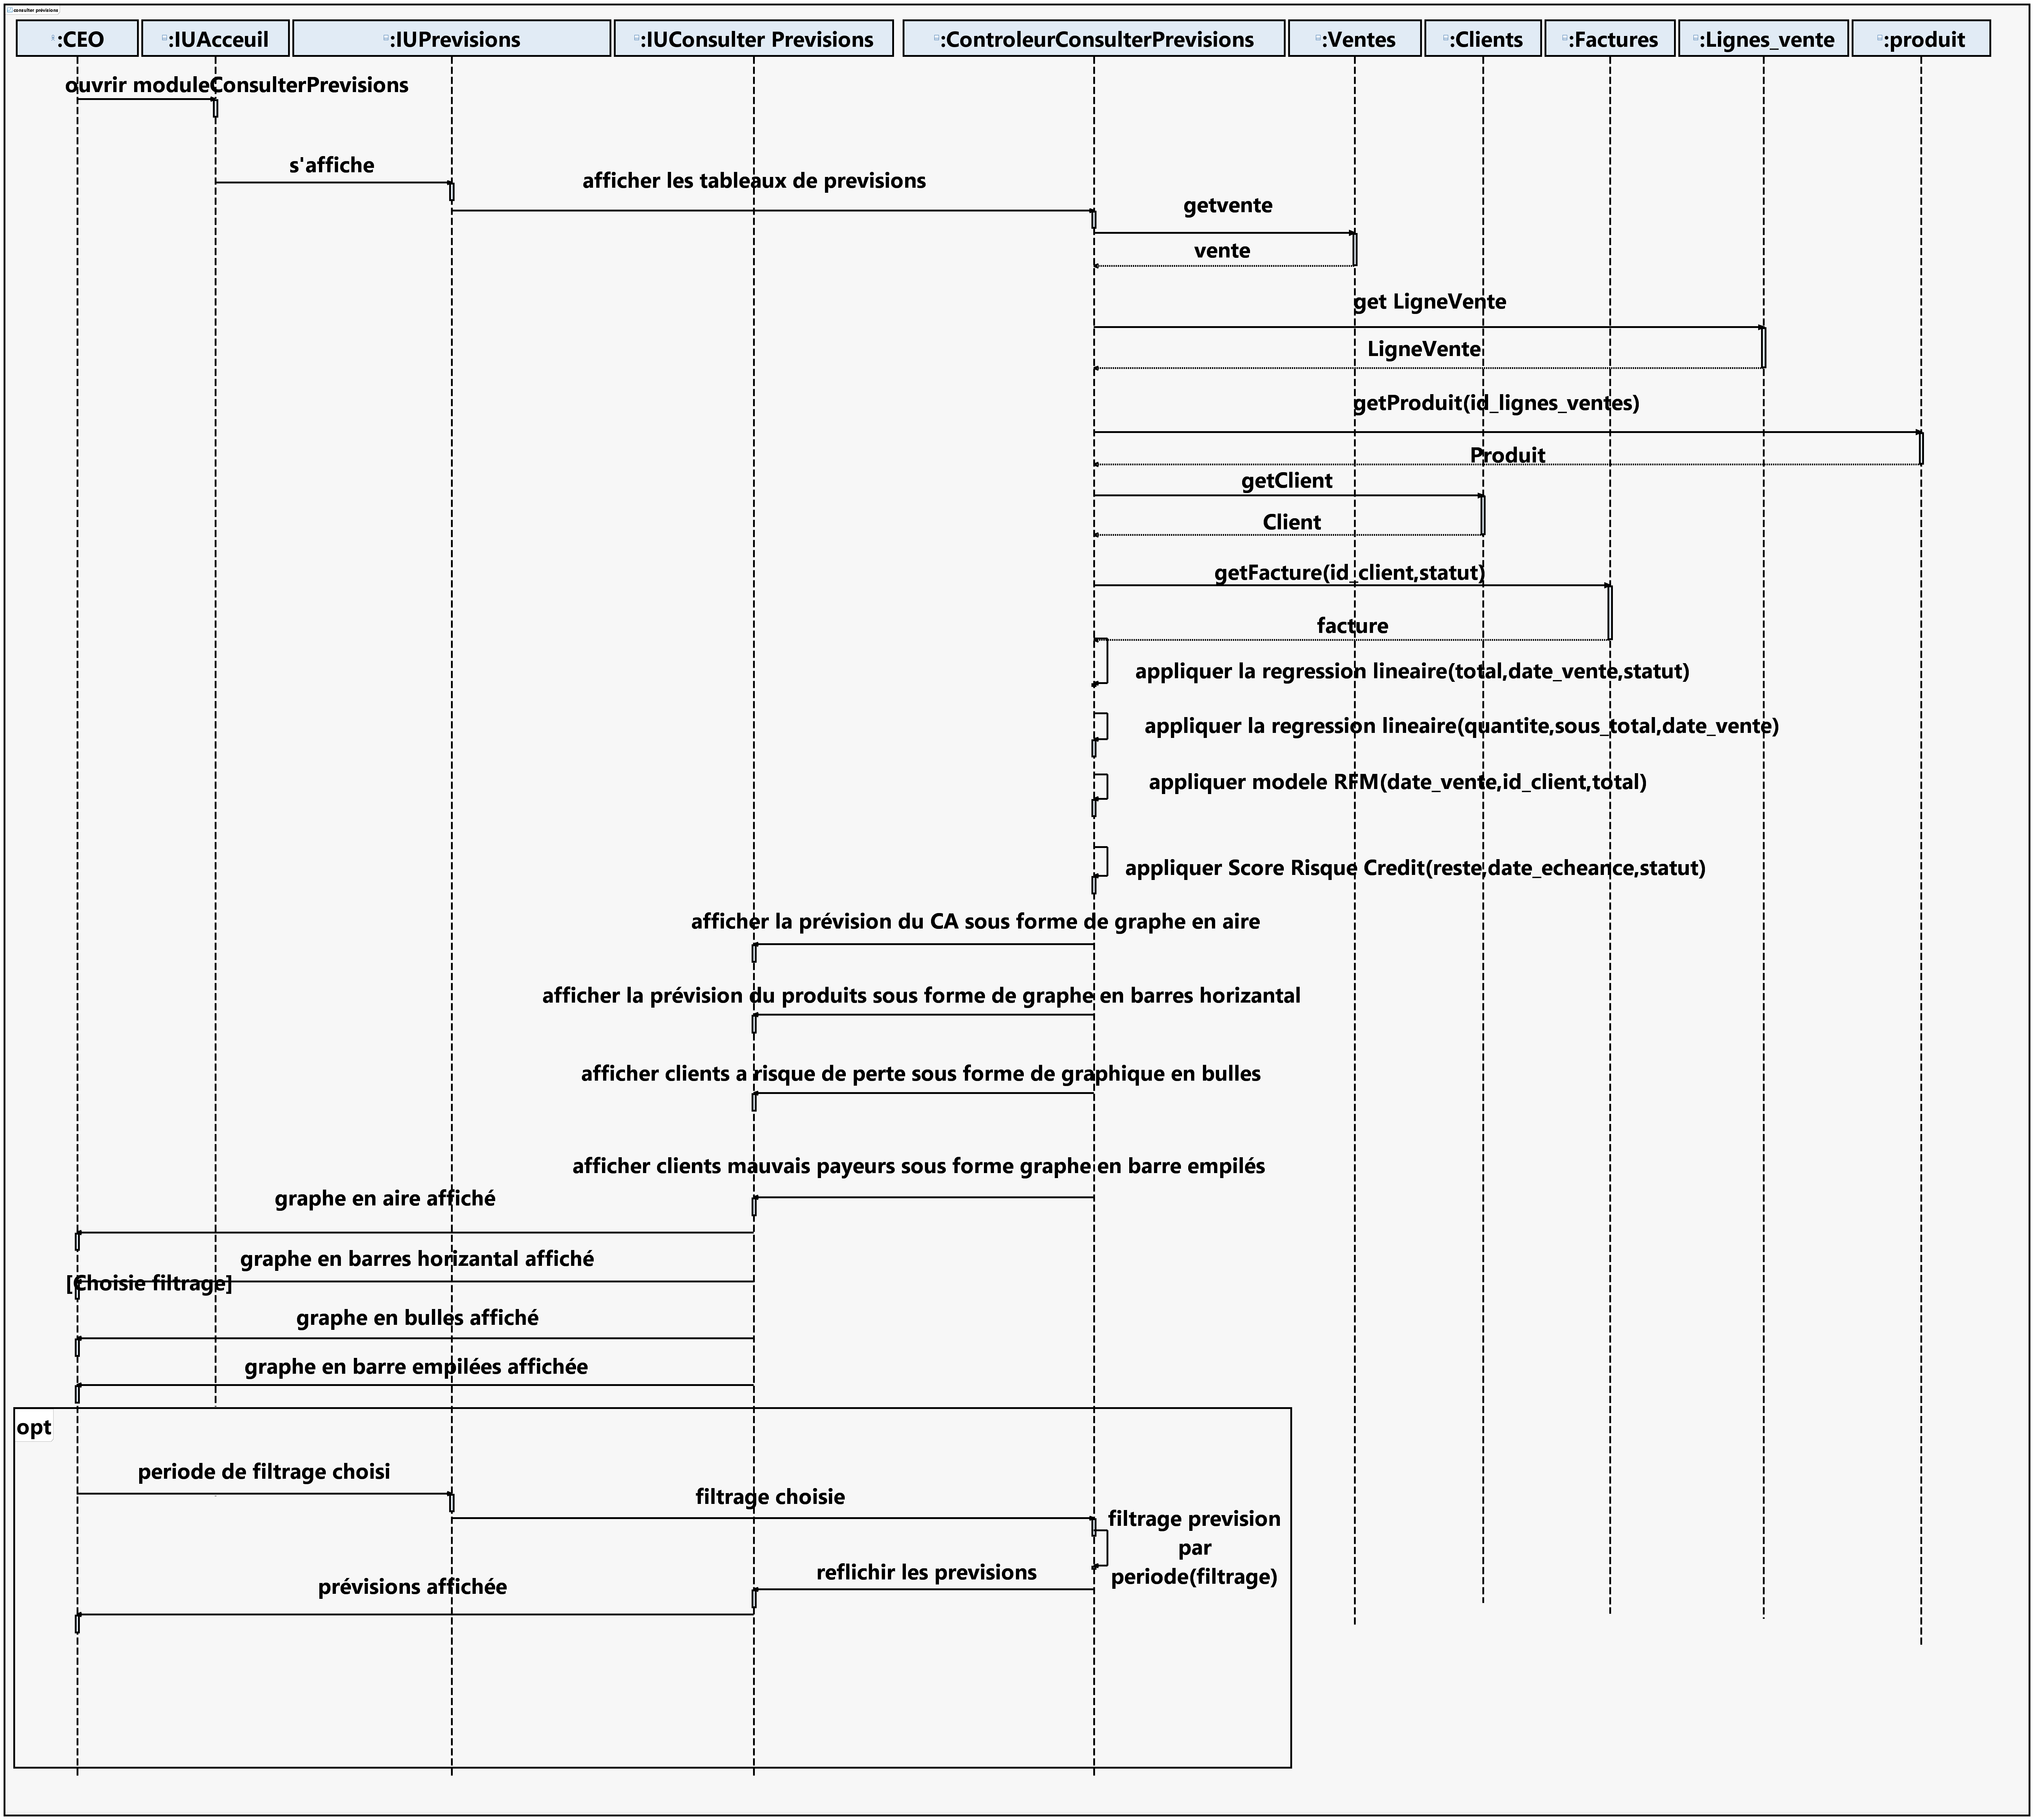
\includegraphics[width=1.15\textwidth, height=0.78\textheight]{images/MC_DiagrammeSéquenceConsulterprevisions_1.png}%
  }
  \caption{Diagramme de séquence pour le cas d'utilisation Consulter prévisions}
  \label{fig:Consulterprévisions}
\end{figure}

\needspace{0.88\textheight}
\subsection{Diagramme de Classe du Cas D'utilisation Consulter prévisions}

\begin{figure}[H]
  \centering
  \makebox[\textwidth][c]{%
    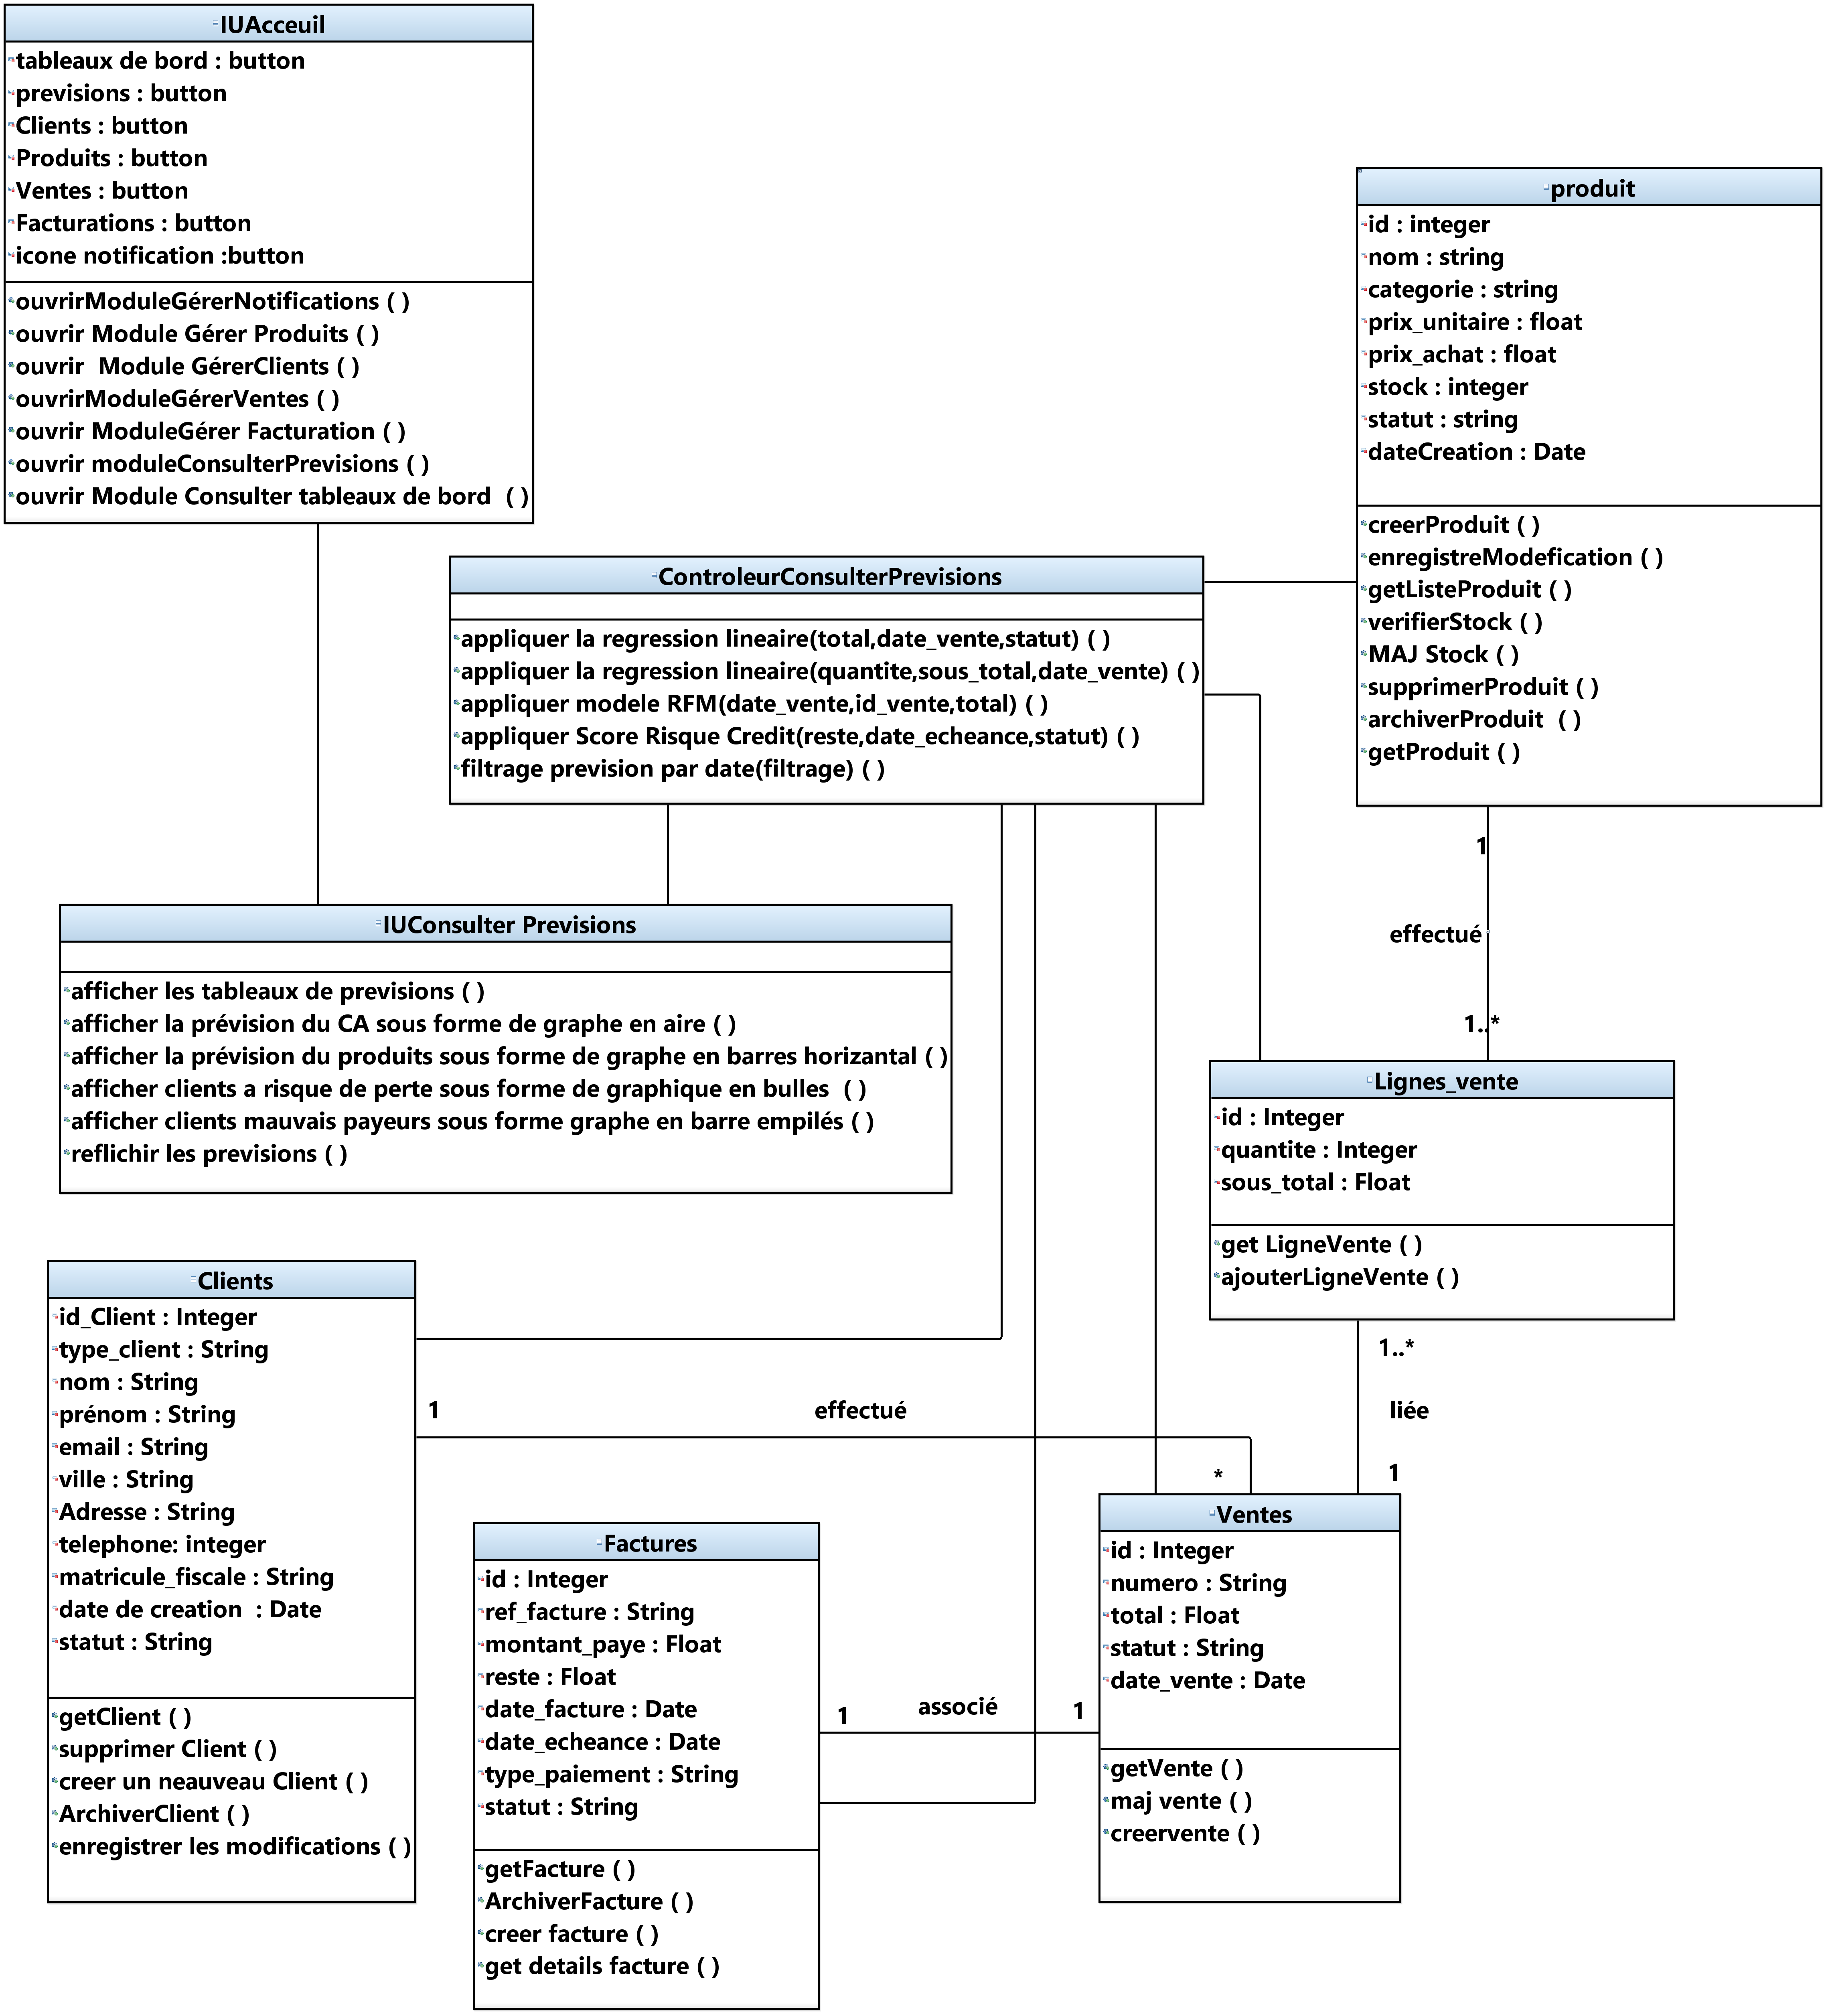
\includegraphics[width=1.05\textwidth, height=0.85\textheight]{images/MC_DiagrammeClasseConsulterPrévisions (1).png}%
  }
  \caption{Diagramme de classe pour le cas d'utilisation Consulter prévisions}
  \label{fig:classeprévisions}
\end{figure}

\newpage

\section{Diagramme de Classes Entité du systéme }
\begin{figure}[H]
  \centering
  \makebox[\textwidth][c]{%
    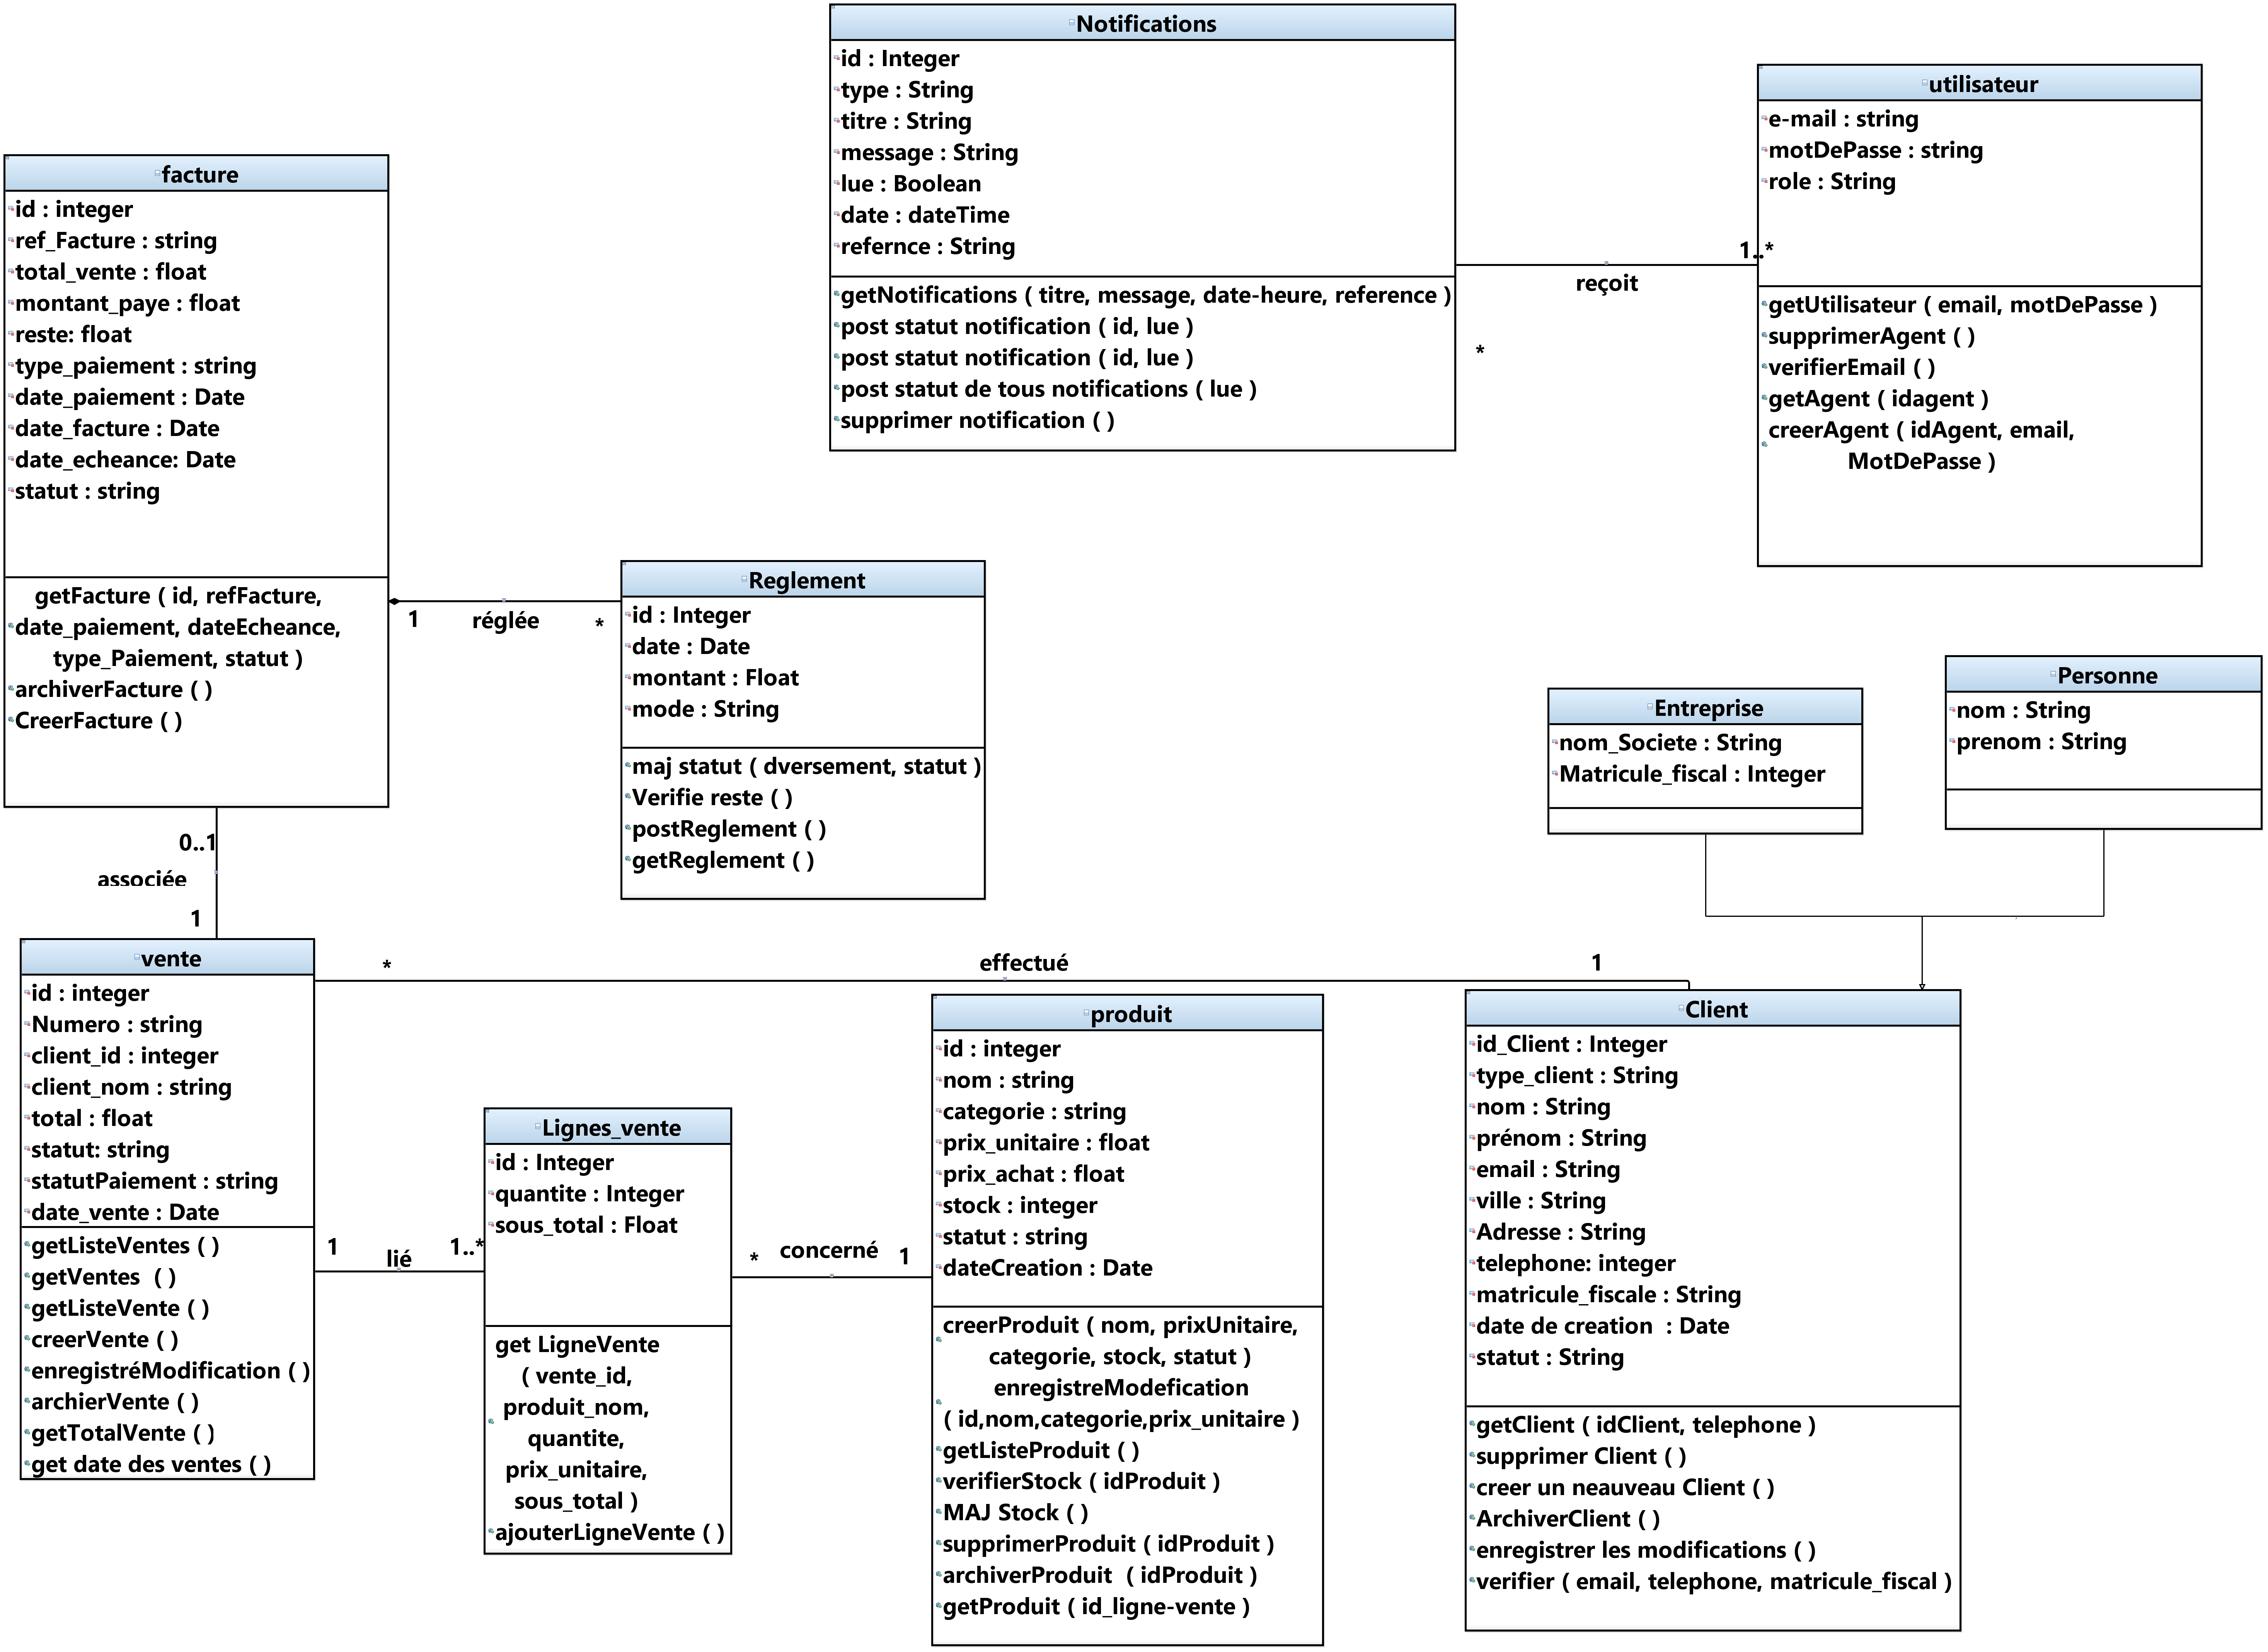
\includegraphics[width=1.05\textwidth, height=0.85\textheight]{images/Packagevierge_DiagrammeClasse.png}%
  }
  \caption{Diagramme de classes}
  \label{fig:diagrammeClasse}
\end{figure}

\newpage

\section{Schéma de la Base de Données}

\sloppy

\noindent\textbf{Utilisateur (}\underline{id}, email, mot\_de\_passe, role\textbf{)}

\vspace{6pt}
\noindent\textbf{Clients (}\underline{id}, type\_client, nom, prenom, email, telephone, ville, adresse, matricule\_fiscal, date\_creation, statut\textbf{)}

\vspace{6pt}
\noindent\textbf{Produits (}\underline{id}, nom, categories, prix\_achat, prix\_vente, stock, date\_creation, statut\textbf{)}

\vspace{6pt}
\noindent\textbf{Ventes (}\underline{id}, numero, total, date\_vente, statut, \#id\_client\textbf{)}

\vspace{6pt}
\noindent\textbf{Ligne\_vente (}\underline{id}, sous\_total, quantite, \#id\_produit, \#id\_vente\textbf{)}

\vspace{6pt}
\noindent\textbf{Facturations (}\underline{id}, ref\_facture, total, montant\_paye, reste,date\_facture, date\_echeance,
date\_paiement, type\_paiement, statut, \#id\_vente\textbf{)}

\vspace{6pt}
\noindent\textbf{Reglements (}\underline{id}, numero, date\_reglement, montant, mode, \#id\_facturation\textbf{)}

\vspace{6pt}
\noindent\textbf{Notifications (}\underline{id}, type, titre, message, lue, date, reference\textbf{)}

\vspace{6pt}
\noindent\textbf{ligne\_notif(}\underline{id}, id\_notifications, id\_utilisateur\textbf{)}

\fussy

\newpage

\section{Diagramme de Déploiement}

\begin{figure}[H]
  \centering
  \makebox[\textwidth][c]{%
    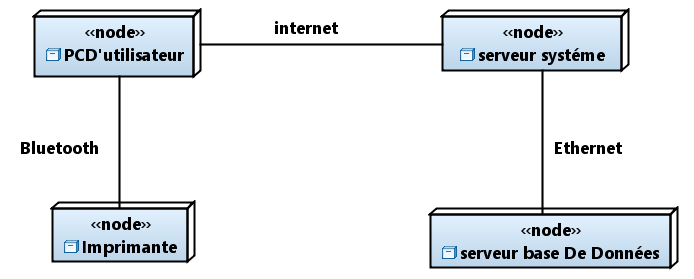
\includegraphics[width=1.2\textwidth, keepaspectratio]{images/MC1_DiagrammeDéploiement_1.png}%
  }
  \caption{Diagramme de déploiement}
  \label{fig:diagramme-deploiement}
\end{figure}

\noindent
Ce diagramme de déploiement présente l'architecture physique du notre système. Il est composé de quatre nœuds : le \textbf{PC de l'utilisateur}, le \textbf{serveur système}, le \textbf{serveur de base de données} et l'\textbf{imprimante}. Le PC de l'utilisateur communique avec le serveur système via \textbf{Internet}, le serveur système est relié au serveur de base de données via \textbf{Ethernet}, et le PC de l'utilisateur est connecté à l'imprimante via \textbf{Bluetooth}.

\section*{Conclusion}
Ce chapitre a exposé la conception de notre systéme , en incluant l'architecture logique adopté, les diagrammes de séquence, les diagrammes de  Classes, les indicateurs clés de performance, ainsi que le schéma de la base.
tous ces éléments constituent une base solide pour Les détails sur l'implémentation de l'application seront fournis dans le chapitre suivant.


\mychapter{Exploitation des données}
%----------------------------------
\section{Introduction}
%----------------------------------

Dans ce chapitre, nous présentons les deux composantes analytiques de notre système :
la Business Intelligence (BI) et l'Intelligence Artificielle (IA). La BI regroupe
l'ensemble des tableaux de bord interactifs et des indicateurs de performance permettant
le pilotage de l'activité commerciale en temps réel. L'IA, quant à elle, est mise en
œuvre à travers un module de prévision des ventes basé sur la régression linéaire,
visant à anticiper les tendances futures de l'activité.

%----------------------------------
\section{Business Intelligence}
%----------------------------------

Face à la concurrence croissante et à la complexité des marchés, les entreprises
ne peuvent plus se contenter de gérer leurs données a posteriori. L'analyse prédictive
est devenue un levier essentiel pour anticiper les tendances, identifier les risques
et optimiser la prise de décision.

\subsection{Définition}

La Business Intelligence (BI) est un processus technologique d'analyse des données
et de présentation d'informations pour aider à prendre des décisions sures,
Dans le cadre de notre système, la BI englobe l'ensemble des outils et méthodologies
mis en place des modules de ventes, clients, produits et facturation. Ces données
sont ensuite traitées et préparées pour l'analyse, afin de créer des tableaux de bord
interactifs, des indicateurs de performance (KPIs) et des graphiques de visualisation,
afin de prendre des décisions basées sur des données concrètes \cite{oracle_bi}.

%----------------------------------
\subsection{Application de la méthode GIMSI}
%----------------------------------

La structure de notre partie BI s'appuie sur la méthode GIMSI, dont nous avons
appliqué 7 étapes réparties sur 3 phases. Chacune de ces étapes a été traitée
dans les différents chapitres du présent rapport, comme détaillé dans le
tableau~\ref{tab:gimsi}.

\vspace{6pt}

\begin{longtable}{|>{\centering\arraybackslash}p{3cm}|>{\centering\arraybackslash}p{0.8cm}|>{\bfseries\raggedright\arraybackslash}p{3.5cm}|>{\raggedright\arraybackslash}p{5cm}|}
\hline
\rowcolor{blue!20}
\textcolor{black}{\textbf{Phase}} &
\textcolor{black}{\textbf{Étape}} &
\textcolor{black}{\textbf{Intitulé}} &
\textcolor{black}{\textbf{Description}} \\
\hline
\endfirsthead
\hline
\rowcolor{blue!20}
\textcolor{black}{\textbf{Phase}} &
\textcolor{black}{\textbf{Étape}} &
\textcolor{black}{\textbf{Intitulé}} &
\textcolor{black}{\textbf{Description}} \\
\hline
\endhead
\multirow{2}{3cm}{\centering\textbf{Phase 1}\\\textbf{Identification}} &
1 & Environnement de l'entreprise &
Analyse de l'environnement économique et de la stratégie afin de définir le périmètre
et la portée du projet (voir Chapitre~1). \\
\cline{2-4}
& 2 & Identification de l'entreprise &
Identification des structures, processus, activités et acteurs concernés
(voir Chapitres~1 et~2). \\
\hline
\multirow{3}{3cm}{\centering\textbf{Phase 2}\\\textbf{Conception}} &
3 & Définition des objectifs &
Définition des objectifs décisionnels en lien avec les besoins stratégiques
(voir Chapitre~2). \\
\cline{2-4}
& 4 & Construction du tableau de bord &
Conception des tableaux de bord adaptés aux besoins de chaque acteur
(voir Chapitre~3). \\
\cline{2-4}
& 5 & Choix des indicateurs &
Sélection des indicateurs clés de performance (KPIs) en fonction des objectifs
et du contexte de l'entreprise (voir Chapitre~4). \\
\cline{2-4}
& 7 & Système de tableaux de bord &
Construction et intégration du système complet de tableaux de bord interactifs
(voir Chapitre~4). \\
\hline
\textbf{Phase 3}\newline\textbf{Mise en œuvre} &
9 & Intégration et déploiement &
Déploiement de la solution complète au sein de l'environnement de l'entreprise
(voir Chapitre~5). \\
\hline
\caption{Application de la méthode GIMSI}
\label{tab:gimsi}
\end{longtable}

\subsection*{Conception des Indicateurs Clés de Performances}
\label{sec:ch3:kpi}
\addcontentsline{toc}{subsection}{Conception des Indicateurs Clés de Performances}

\vspace{6pt}

\begin{longtable}{|>{\centering\arraybackslash\bfseries}p{2.5cm}|>{\raggedright\arraybackslash}p{4cm}|>{\raggedright\arraybackslash}p{4cm}|>{\centering\arraybackslash}p{1.8cm}|>{\centering\arraybackslash}p{1.5cm}|}
\hline
\rowcolor{blue!20}
\textcolor{black}{\textbf{KPI}} &
\textcolor{black}{\textbf{Description}} &
\textcolor{black}{\textbf{Formule}} &
\textcolor{black}{\textbf{Graphique}} &
\textcolor{black}{\textbf{Couleur}} \\
\hline
\endfirsthead
\hline
\rowcolor{blue!20}
\textcolor{black}{\textbf{KPI}} &
\textcolor{black}{\textbf{Description}} &
\textcolor{black}{\textbf{Formule}} &
\textcolor{black}{\textbf{Graphique}} &
\textcolor{black}{\textbf{Couleur}} \\
\hline
\endhead
Chiffres d'affaires total &
Cet indicateur est chargé d'afficher le montant global de l'ensemble des ventes actives. &
CA total = Somme des ventes actives &
Carte avec icône &
\colorswatch{blue!70!black} \\
\hline
Chiffres d'affaires mensuel &
Cet indicateur est chargé d'afficher le montant des ventes effectuées dans le mois souhaité. &
CA mensuel = Somme des ventes du mois souhaité &
Carte avec icône &
\colorswatch{blue!50} \\
\hline
Panier Moyen &
Cet indicateur est chargé de mesurer le revenu moyen généré par chaque vente effectuée. &
Panier moyen = CA Total / Nombre de ventes &
Carte avec icône &
\colorswatch{violet} \\
\hline
\textcolor{blue!70!black}{Taux de Croissance} &
Cet indicateur est chargé de mesurer la variance du chiffre d'affaires par rapport au mois précédent. &
Croissance = [CA(n) - CA(n-1)] / CA(n-1) x 100 &
Carte avec icône &
\begin{tabular}[c]{@{}c@{}}
\colorswatch{green!60!black}\\[-2pt]
{\tiny Vert si positif}\\[4pt]
\colorswatch{red!70}\\[-2pt]
{\tiny Rouge si négatif}\\[4pt]
\colorswatch{gray!50}\\[-2pt]
{\tiny Gris si nul}
\end{tabular} \\
\hline
\textcolor{blue!70!black}{Taux de marge} &
Cet indicateur est chargé de mesurer le gain réalisé sur les ventes enregistrées, correspondant à la différence entre le chiffre d'affaires et le coût d'achat. &
Marge brute = quantité x (prix\_vente - prix\_achat)

\vspace{4pt}
Taux de marge = marge brute / (quantité x prix\_vente) x 100 &
Carte avec icône &
\colorswatch{orange!80!black} \\
\hline
\caption{Conception des Indicateurs Clés de Performances}
\label{tab:kpi-generaux}
\end{longtable}

\newpage

\subsection*{Conception des KPIs — Tableau de Bord Chiffre d'Affaires}
\addcontentsline{toc}{subsection}{Conception des KPIs — Tableau de Bord Chiffre d'Affaires}

\begin{longtable}{|>{\centering\arraybackslash\bfseries}p{2.5cm}|>{\raggedright\arraybackslash}p{3.5cm}|>{\raggedright\arraybackslash}p{4cm}|>{\centering\arraybackslash}p{1.8cm}|>{\centering\arraybackslash}p{1.5cm}|}
\hline
\rowcolor{blue!20}
\textcolor{black}{\textbf{KPI}} &
\textcolor{black}{\textbf{Description}} &
\textcolor{black}{\textbf{Formule}} &
\textcolor{black}{\textbf{Graphique}} &
\textcolor{black}{\textbf{Couleur}} \\
\hline
\endfirsthead
\hline
\rowcolor{blue!20}
\textcolor{black}{\textbf{KPI}} &
\textcolor{black}{\textbf{Description}} &
\textcolor{black}{\textbf{Formule}} &
\textcolor{black}{\textbf{Graphique}} &
\textcolor{black}{\textbf{Couleur}} \\
\hline
\endhead
Évolution du chiffre d'affaires &
Ce graphique est chargé d'afficher l'évolution du chiffre d'affaires et du volume de ventes enregistrés mois par mois ou semaine par semaine. &
Chiffres d'affaire = Somme de total (par mois/par semaine)

\vspace{4pt}
Nombres des ventes = Count nombre ventes (par mois/par semaine) &
Graphique combiné (Barres + Aires)

\vspace{4pt}
\textit{Info\_bulle} (affiche le CA et nombre de ventes) &
\begin{tabular}[c]{@{}c@{}}
\colorswatch{blue!70!black}\\[-2pt]
{\tiny Barres}\\[6pt]
\colorswatch{blue!30}\\[-2pt]
{\tiny Aire}
\end{tabular} \\
\hline
Anomalies CA &
Est chargé d'afficher les jours anormaux du chiffre d'affaires détectés sur la période. &
Moyenne = CA/jour / nombre-jour

\vspace{4pt}
Ecart\_type = racine( somme(CA\_jour - Moyenne)\textsuperscript{2} / n )

\vspace{4pt}
Z\_score = (CA/jour - moyenne) / ecart\_type &
Graphique en aires &
\begin{tabular}[c]{@{}c@{}}
\colorswatch{blue!30}\\[-2pt]
{\tiny Aire normale}\\[4pt]
\colorswatch{red!80}\\[-2pt]
{\tiny Pic anormal}\\[4pt]
\colorswatch{orange!80}\\[-2pt]
{\tiny Creux anormal}
\end{tabular} \\
\hline
Top 5 Produits par Chiffre d'affaires &
Cette section est chargée de classer et afficher les 5 produit ayant généré plus de chiffres d'affaires. &
CA Total d'affaire par produit = Somme de sous total (par produit)

\vspace{4pt}
Trié en ordre décroissant (5 premiers résultats) &
Liste classée &
\\
\hline
Répartition du CA Par produit/Catégorie &
Cette section est chargée d'afficher la contribution proportionnelle de chaque produit au chiffre d'affaires regroupé par catégories. &
Répartition du CA d'affaire par produit = CA par produit / CA total

\vspace{4pt}
Répartition du CA d'affaires par Catégories = CA par catégories / CA total &
Diagramme en secteurs

\vspace{4pt}
\textit{Info\_bulle} (affiche nom de produit + CA en TND)

\vspace{4pt}
\textit{Panneau de légende} (affiche nom de catégorie + CA + répartition) &
\begin{tabular}[c]{@{}c@{}}
\colorswatch{blue!70!black}\\[-2pt]
{\tiny Rang 1}\\[4pt]
\colorswatch{blue!55}\\[-2pt]
{\tiny Rang 2}\\[4pt]
\colorswatch{blue!40}\\[-2pt]
{\tiny Rang 3}\\[4pt]
\colorswatch{blue!25}\\[-2pt]
{\tiny Rang 4}\\[4pt]
\colorswatch{blue!10}\\[-2pt]
{\tiny Rang 5}
\end{tabular} \\
\hline
\caption{Conception des KPIs — Tableau de Bord Chiffre d'Affaires}
\label{tab:kpi-ca}
\end{longtable}

\newpage

\subsection*{Conception des KPIs — Tableau de Bord Clients}
\addcontentsline{toc}{subsection}{Conception des KPIs — Tableau de Bord Clients}

\begin{longtable}{|>{\centering\arraybackslash\bfseries}p{2.5cm}|>{\raggedright\arraybackslash}p{3.5cm}|>{\raggedright\arraybackslash}p{4cm}|>{\centering\arraybackslash}p{1.8cm}|>{\centering\arraybackslash}p{1.5cm}|}
\hline
\rowcolor{blue!20}
\textcolor{black}{\textbf{KPI}} &
\textcolor{black}{\textbf{Description}} &
\textcolor{black}{\textbf{Formule}} &
\textcolor{black}{\textbf{Graphique}} &
\textcolor{black}{\textbf{Couleur}} \\
\hline
\endfirsthead
\hline
\rowcolor{blue!20}
\textcolor{black}{\textbf{KPI}} &
\textcolor{black}{\textbf{Description}} &
\textcolor{black}{\textbf{Formule}} &
\textcolor{black}{\textbf{Graphique}} &
\textcolor{black}{\textbf{Couleur}} \\
\hline
\endhead
Top 5 clients par Chiffre d'affaires &
Cette section est chargée de classer et afficher les 5 clients ayant généré plus de chiffres d'affaires. &
CA Total d'affaire par clients = Somme de total (par clients)

\vspace{4pt}
Trié en ordre décroissant (5 premiers résultats) &
Liste classée &
\\
\hline
Répartition du CA Par Client/Type &
Cette section est chargée d'afficher la contribution proportionnelle de chaque client au chiffre d'affaires segmenté par type de client. &
Répartition du CA d'affaire par client = CA par client / CA total

\vspace{4pt}
Répartition du CA d'affaires par types = CA par types / CA total &
Diagramme en secteurs

\vspace{4pt}
\textit{Info\_bulle} (affiche nom de client + CA en TND)

\vspace{4pt}
\textit{Panneau de légende} (affiche nom de type + CA + répartition) &
\begin{tabular}[c]{@{}c@{}}
\colorswatch{blue!70!black}\\[-2pt]
{\tiny Rang 1}\\[4pt]
\colorswatch{blue!55}\\[-2pt]
{\tiny Rang 2}\\[4pt]
\colorswatch{blue!40}\\[-2pt]
{\tiny Rang 3}\\[4pt]
\colorswatch{blue!25}\\[-2pt]
{\tiny Rang 4}\\[4pt]
\colorswatch{blue!10}\\[-2pt]
{\tiny Rang 5}
\end{tabular} \\
\hline
\caption{Conception des KPIs — Tableau de Bord Clients}
\label{tab:kpi-clients}
\end{longtable}

\newpage

\subsection*{Conception des KPIs — Tableau de Bord Facturation}
\addcontentsline{toc}{subsection}{Conception des KPIs — Tableau de Bord Facturation}

\begin{longtable}{|>{\centering\arraybackslash\bfseries}p{2.5cm}|>{\raggedright\arraybackslash}p{3.5cm}|>{\raggedright\arraybackslash}p{4cm}|>{\centering\arraybackslash}p{1.8cm}|>{\centering\arraybackslash}p{1.5cm}|}
\hline
\rowcolor{blue!20}
\textcolor{black}{\textbf{KPI}} &
\textcolor{black}{\textbf{Description}} &
\textcolor{black}{\textbf{Formule}} &
\textcolor{black}{\textbf{Graphique}} &
\textcolor{black}{\textbf{Couleur}} \\
\hline
\endfirsthead
\hline
\rowcolor{blue!20}
\textcolor{black}{\textbf{KPI}} &
\textcolor{black}{\textbf{Description}} &
\textcolor{black}{\textbf{Formule}} &
\textcolor{black}{\textbf{Graphique}} &
\textcolor{black}{\textbf{Couleur}} \\
\hline
\endhead
Répartition des factures par Statut &
Cet indicateur est chargé de visualiser la distribution des factures selon leur statut de paiement (payé/non payé/Partiellement payé). &
Montant des factures par statut = Somme des factures par statut

\vspace{4pt}
Part des factures par statut = (Montant par statut / Montant total des factures) x 100

\vspace{4pt}
Nombre de factures par type = Count factures (par statut) &
Graphique en anneau (donut chart)

\vspace{4pt}
\textit{Centre de graphique} affiche le nombre total de factures + montant total en TND

\vspace{4pt}
\textit{Info\_bulle} (affiche nom de statut + montant + nombre) &
\begin{tabular}[c]{@{}c@{}}
\colorswatch{green!60!black}\\[-2pt]
{\tiny payé}\\[6pt]
\colorswatch{orange!80}\\[-2pt]
{\tiny partiellement\_payé}\\[6pt]
\colorswatch{red!70}\\[-2pt]
{\tiny non payé}
\end{tabular} \\
\hline
Répartition des factures par Type &
Cet indicateur est chargé d'afficher la répartition entre les paiements en Comptant et en Facilité sur l'ensemble des factures. &
Montant des factures par type = Somme des factures par type

\vspace{4pt}
Part des factures par type = (Montant par type / Montant total des factures) x 100

\vspace{4pt}
Nombre de factures (avec au moins un paiement enregistré) par type = Count facture (par type) &
Graphique en anneau (donut chart)

\vspace{4pt}
\textit{Centre de graphique} affiche le nombre de factures + montant total en TND

\vspace{4pt}
\textit{Info\_bulle} (affiche nom de type + montant + nombre) &
\colorswatch{green!60!black} \\
\hline
Répartition des règlements par mode &
Cet indicateur est chargé d'afficher la distribution des règlements selon le mode de paiement (Espèces, Chèque, Virement, Carte bancaire, etc.). &
Montant des règlements par mode = Somme des règlements par mode

\vspace{4pt}
Part des règlements par mode = (Montant par mode / Montant total des règlements) x 100

\vspace{4pt}
Nombre de règlements par mode = Count règlements (par mode) &
Graphique en anneau (donut chart)

\vspace{4pt}
\textit{Centre de graphique} affiche le nombre de règlements + montant total en TND

\vspace{4pt}
\textit{Info\_bulle} (affiche nom de mode + montant + nombre) &
\begin{tabular}[c]{@{}c@{}}
\colorswatch{green!60!black}\\[-2pt]
{\tiny vert si Espèces}\\[4pt]
\colorswatch{blue!60}\\[-2pt]
{\tiny bleu si carte bancaire}\\[4pt]
\colorswatch{orange!80}\\[-2pt]
{\tiny orange si chèque}\\[4pt]
\colorswatch{violet}\\[-2pt]
{\tiny violet si virement}
\end{tabular} \\
\hline
Total encaissé &
Est chargé d'afficher le montant des paiements effectivement reçus (réglées). &
Total encaissé = Somme des factures payé + partie encaissée de partiellement payé &
Panneau de légende &
\colorswatch{green!60!black} \\
\hline
Total attendu &
Est chargé d'afficher le montant des paiements non encore reçus (attente de règlements). &
Total attendu = Somme des factures non payé + solde restant de partiellement payé &
Panneau de légende &
\colorswatch{orange!80} \\
\hline
Top 5 Clients fidèles &
Cette section est chargée de classer et afficher les clients fidèles ayant généré le plus nombres de ventes. &
Clients fidèles = Count nombre des ventes (par client)

\vspace{4pt}
Trié en ordre décroissant (5 premiers résultats) &
Liste classée &
\begin{tabular}[c]{@{}c@{}}
\colorswatch{blue!70!black}\\[-2pt]
{\tiny rang1}\\[4pt]
\colorswatch{blue!55}\\[-2pt]
{\tiny rang2}\\[4pt]
\colorswatch{blue!40}\\[-2pt]
{\tiny rang3}\\[4pt]
\colorswatch{blue!25}\\[-2pt]
{\tiny rang4}\\[4pt]
\colorswatch{blue!10}\\[-2pt]
{\tiny rang5}
\end{tabular} \\
\hline
\caption{Conception des KPIs — Tableau de Bord Facturation}
\label{tab:kpi-facturation}
\end{longtable}

\newpage

\subsection*{Conception des KPIs — Tableau de Bord Prévisions}
\addcontentsline{toc}{subsection}{Conception des KPIs — Tableau de Bord Prévisions}

\begin{longtable}{|>{\centering\arraybackslash\bfseries}p{2cm}|>{\raggedright\arraybackslash}p{3cm}|>{\raggedright\arraybackslash}p{2.8cm}|>{\centering\arraybackslash}p{2cm}|>{\centering\arraybackslash}p{2cm}|>{\centering\arraybackslash}p{1.5cm}|}
\hline
\rowcolor{blue!20}
\textcolor{black}{\textbf{KPI}} &
\textcolor{black}{\textbf{Description}} &
\textcolor{black}{\textbf{Algorithme}} &
\textcolor{black}{\textbf{Type IA}} &
\textcolor{black}{\textbf{Graphique}} &
\textcolor{black}{\textbf{Couleur}} \\
\hline
\endfirsthead
\hline
\rowcolor{blue!20}
\textcolor{black}{\textbf{KPI}} &
\textcolor{black}{\textbf{Description}} &
\textcolor{black}{\textbf{Algorithme}} &
\textcolor{black}{\textbf{Type IA}} &
\textcolor{black}{\textbf{Graphique}} &
\textcolor{black}{\textbf{Couleur}} \\
\hline
\endhead
Prévision CA &
Cette section est chargée d'afficher les prévisions futures du CA basées sur les tendances historiques. &
Régression Linéaire &
ML supervisé &
Graphique en courbe aires &
\\
\hline
Prévision ventes par produit &
Cette section est chargée de prédire la quantité et le CA pour chaque produit à partir de son historique. &
Régression Linéaire &
ML supervisé &
Graphique en barres horizontales &
\\
\hline
Clients à risque de perte &
Cette section permet d'identifier les clients inactifs ou en baisse. &
Modèle RFM (Récence, Fréquence, Montant) &
ML non supervisé (scoring) &
Graphique en bulles &
\begin{tabular}[c]{@{}c@{}}
\colorswatch{red!80}\\[-2pt]
{\tiny Risque}\\[4pt]
\colorswatch{orange!80}\\[-2pt]
{\tiny Critique}\\[4pt]
\colorswatch{green!60!black}\\[-2pt]
{\tiny Actif}
\end{tabular} \\
\hline
Clients mauvais payeurs &
Cette section est chargée de calculer et d'afficher le score pour chaque client ayant des factures en retard de paiement. &
Score crédit pondéré &
Scoring expert &
Graphique en barres empilées &
\begin{tabular}[c]{@{}c@{}}
\colorswatch{red!80}\\[-2pt]
{\tiny Critique}\\[4pt]
\colorswatch{orange!80}\\[-2pt]
{\tiny Élevé}\\[4pt]
\colorswatch{yellow!80!black}\\[-2pt]
{\tiny Faible}
\end{tabular} \\
\hline
\caption{Conception des KPIs — Tableau de Bord Prévisions}
\label{tab:kpi-previsions}
\end{longtable}

\newpage

\textbf{Étape 7 --- Système de tableaux de bord :}
Dans cette étape, nous avons construit et intégré le système complet de tableaux de
bord interactifs, en assurant la cohérence globale des indicateurs et des
visualisations. Nous présentons ci-dessous des exemples représentatifs des graphiques
utilisés dans chaque tableau de bord.

%--- Tableau de bord CA ---
\subsubsection*{Tableau de bord — Chiffre d'affaires}

\begin{figure}[H]
  \centering
  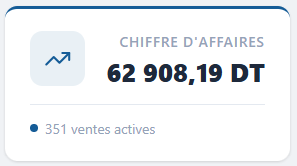
\includegraphics[width=0.6\textwidth]{images/tdb_ca_card.png}
  \caption{Indicateur KPI — Chiffre d'affaires total}
\end{figure}

Nous avons opté pour une \textbf{carte avec icône} pour afficher les indicateurs
synthétiques tels que le chiffre d'affaires total, le panier moyen et le taux de
croissance. Ce format permet une lecture immédiate des valeurs clés sans interprétation
visuelle supplémentaire.

\begin{figure}[H]
  \centering
  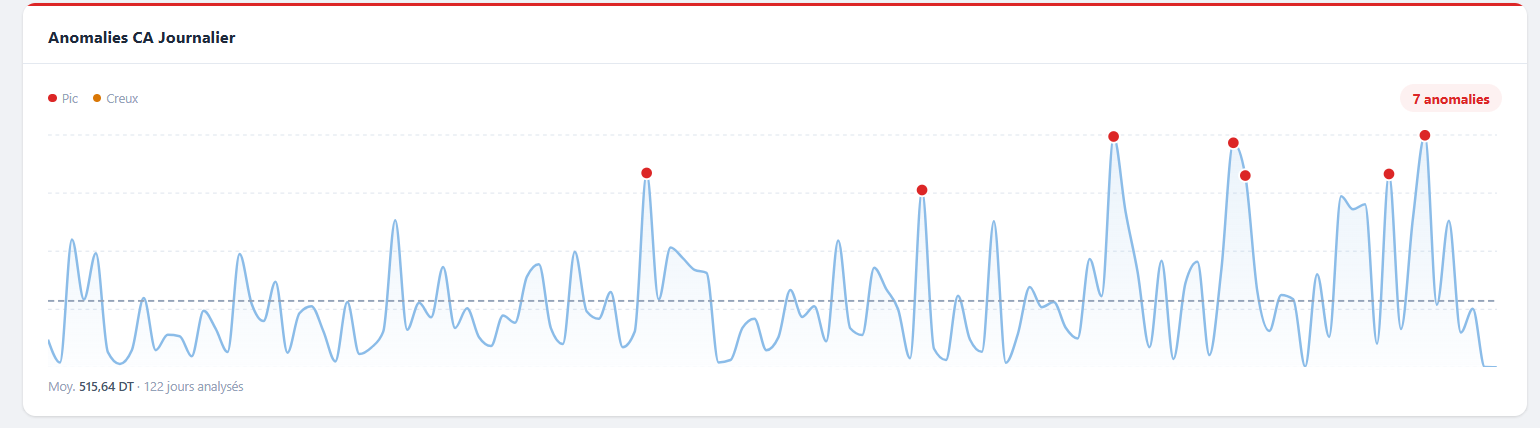
\includegraphics[width=\textwidth]{images/tdb_ca_anomalies.png}
  \caption{Anomalies CA Journalier — Graphique en courbe avec détection de pics}
\end{figure}

Nous avons choisi un \textbf{graphique en courbe} pour les anomalies du CA journalier,
car il permet de visualiser l'évolution continue des ventes et de mettre en évidence
les pics anormaux (en rouge) détectés par le Z-score, avec la moyenne affichée en
ligne pointillée comme référence.

\begin{figure}[H]
  \centering
  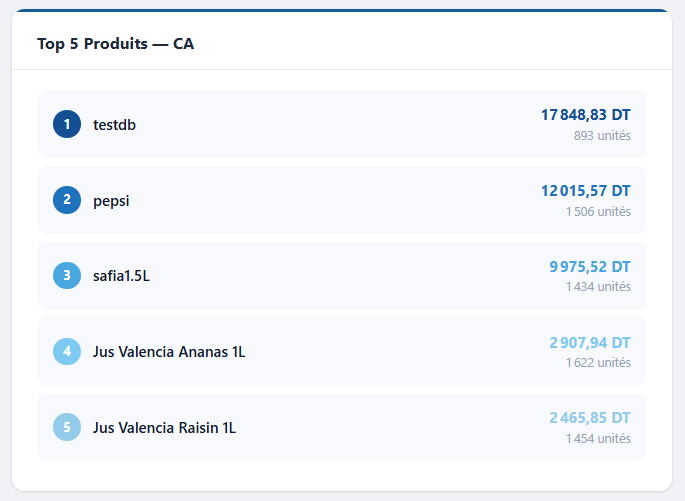
\includegraphics[width=0.65\textwidth]{images/tdb_ca_top5.png}
  \caption{Top 5 Produits par Chiffre d'affaires — Liste classée}
\end{figure}

Nous avons opté pour une \textbf{liste classée} pour le Top 5 des produits, car elle
offre une lecture directe du classement avec le CA et le nombre d'unités vendues pour
chaque produit, sans nécessiter d'interprétation graphique.

\begin{figure}[H]
  \centering
  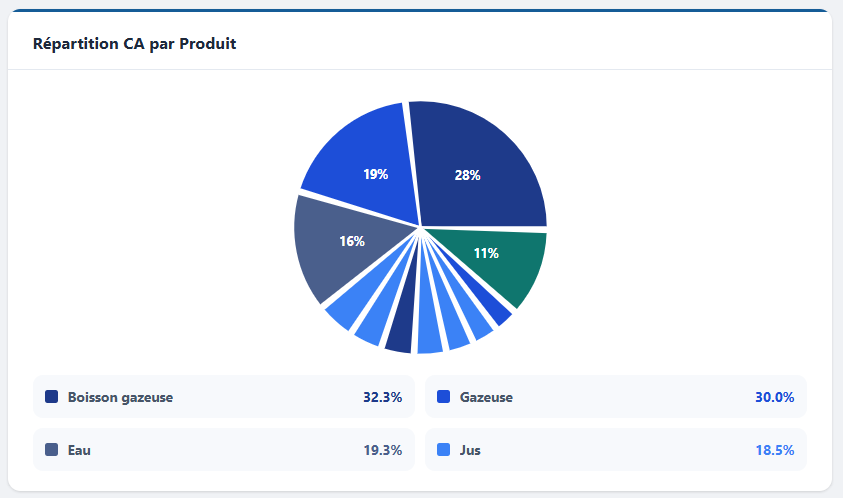
\includegraphics[width=0.65\textwidth]{images/tdb_ca_repartition_produit.png}
  \caption{Répartition du CA par Produit — Diagramme en secteurs}
\end{figure}

Nous avons sélectionné un \textbf{diagramme en secteurs} pour la répartition du CA
par produit et catégorie, car il illustre clairement la contribution proportionnelle
de chaque catégorie (Boisson gazeuse, Gazeuse, Eau, Jus) au chiffre d'affaires global.

%--- Tableau de bord Clients ---
\subsubsection*{Tableau de bord — Clients}

\begin{figure}[H]
  \centering
  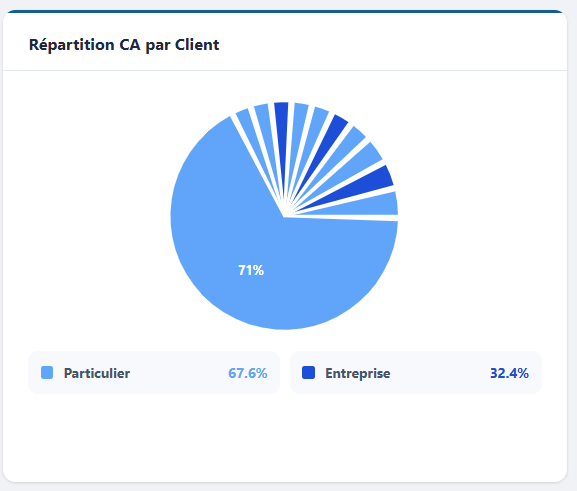
\includegraphics[width=0.65\textwidth]{images/tdb_clients_repartition.png}
  \caption{Répartition du CA par Client — Diagramme en secteurs}
\end{figure}

Nous avons opté pour un \textbf{diagramme en secteurs} pour la répartition du CA par
client et type (Particulier / Entreprise), car il représente efficacement la part de
chaque segment dans le chiffre d'affaires global et permet d'identifier rapidement
les types de clientèle les plus contributifs.

%--- Tableau de bord Facturation ---
\subsubsection*{Tableau de bord — Facturation}

\begin{figure}[H]
  \centering
  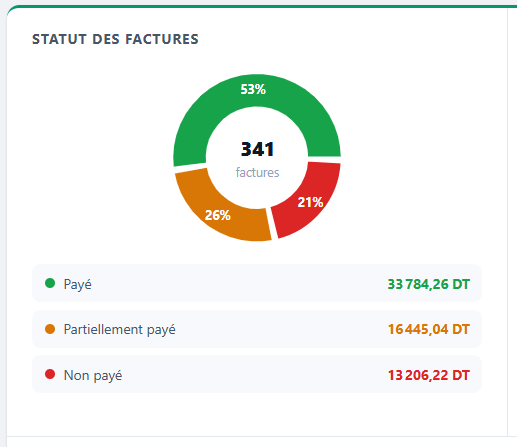
\includegraphics[width=0.55\textwidth]{images/tdb_fact_statut.png}
  \caption{Statut des Factures — Graphique en anneau (donut)}
\end{figure}

Nous avons sélectionné un \textbf{graphique en anneau (donut)} pour le statut des
factures, car il permet d'afficher simultanément le nombre total de factures au centre
(341 factures) et la répartition par statut — Payé (53\%), Partiellement payé (26\%),
Non payé (21\%) — en segments colorés immédiatement lisibles.

\begin{figure}[H]
  \centering
  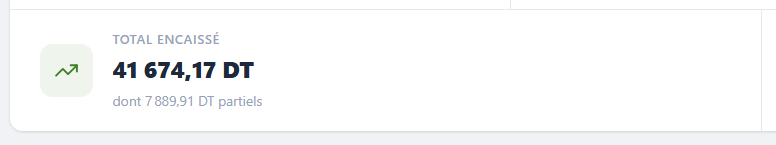
\includegraphics[width=0.65\textwidth]{images/tdb_fact_encaisse.png}
  \caption{Total Encaissé — Carte KPI}
\end{figure}

Nous avons opté pour une \textbf{carte KPI} pour les indicateurs financiers agrégés
tels que le total encaissé et le total attendu, car ce format met en valeur les
montants clés et leur détail (dont la part partielle) de manière synthétique et lisible.


\subsubsection*{Phase 3 : Mise en œuvre}

\textbf{Étape 9 --- Intégration et déploiement de la solution :}
Dans cette étape, nous avons déployé la solution complète au sein de
l'environnement de l'entreprise, en intégrant l'ensemble des modules développés
(voir Chapitre~5, page~\pageref{sec:ch5:impl}).

\newpage

%----------------------------------
\section{Module de Prévision et d'Analyse Intelligente}
%----------------------------------

\subsection{Fondements théoriques}

\subsubsection{L'apprentissage automatique}

L'apprentissage automatique (Machine Learning) est une branche de l'intelligence
artificielle (IA) qui se concentre sur le développement d'algorithmes informatiques
qui s'améliorent automatiquement grâce à l'expérience et à l'utilisation de données.
Il permet à un système d'apprendre à partir de données et de prendre des décisions
ou de faire des prédictions sans avoir été explicitement programmé pour le faire
\cite{datacamp_ml}.

Dans notre projet, il constitue le socle du module de prévision, permettant d'anticiper
le chiffre d'affaires, de segmenter les clients et de détecter les risques de non-paiement.
Les méthodes d'apprentissage se divisent en deux grandes catégories.

\subsubsection{Apprentissage supervisé}

L'apprentissage supervisé est une approche de machine learning qui se définit par
l'utilisation d'ensembles de données étiquetés. Ces jeux de données sont conçus pour
entraîner ou « superviser » les algorithmes afin qu'ils classifient les données ou
prédisent les résultats avec précision. Cette approche a été appliquée dans notre
projet pour prévoir le chiffre d'affaires et les ventes par produit \cite{ibm_supervised}.

\subsubsection{Apprentissage non supervisé}

L'apprentissage non supervisé utilise des algorithmes de machine learning pour analyser
et regrouper des ensembles de données non étiquetés. Ces algorithmes découvrent des
modèles cachés dans les données sans avoir besoin d'intervention humaine
\cite{ibm_supervised}.
Dans ce projet, cette approche permet de détecter les clients à risque et les mauvais
payeurs.

\subsubsection{Outils d'analyse intelligente}

Le tableau~\ref{tab:algorithmes} présente les principaux algorithmes mis en œuvre
dans notre module de prévision et d'analyse intelligente.

\vspace{6pt}

\begin{longtable}{|>{\bfseries\raggedright\arraybackslash}p{3.5cm}|>{\raggedright\arraybackslash}p{9cm}|}
\hline
\rowcolor{blue!20}
\textcolor{black}{\textbf{Algorithme}} &
\textcolor{black}{\textbf{Description}} \\
\hline
\endfirsthead
\hline
\rowcolor{blue!20}
\textcolor{black}{\textbf{Algorithme}} &
\textcolor{black}{\textbf{Description}} \\
\hline
\endhead
Régression Linéaire Simple &
La régression linéaire est une technique d'analyse de données qui prédit la valeur
de données inconnues en utilisant une autre valeur de données apparentée et connue.
Elle modélise mathématiquement la variable dépendante et la variable indépendante
sous forme d'équation linéaire \cite{aws_regression}. \\
\hline
K-Means &
Le clustering k-means est un algorithme d'apprentissage non supervisé utilisé dans
le partitionnement de données, qui regroupe les points de données non étiquetés
en groupes ou clusters \cite{ibm_kmeans}. \\
\hline
RFM &
La segmentation RFM est une approche de classification des clients basée sur la
Récence de leur dernier achat, la Fréquence des transactions et le Montant total
dépensé \cite{dinmo_rfm}. \\
\hline
Isolation Forest &
Isolation Forest est un algorithme de machine learning non supervisé qui identifie
les anomalies dans les données en les isolant via des partitionnements aléatoires
au sein d'un ensemble d'arbres de décision \cite{datacamp_iforest}. \\
\hline
\caption{Outils d'analyse intelligente}
\label{tab:algorithmes}
\end{longtable}


\input{chapitre5}



% ===== WEBOGRAPHIE =====
\renewcommand{\bibname}{Webographie}
\begin{thebibliography}{99}
\raggedright

\bibitem{uml}
Scribd,
\textit{Processus Unifié},
Disponible sur : \url{https://fr.scribd.com/document/682789373/processuc-unifie-2},
Consulté le : avril 2025.

\bibitem{vscode}
Comment Coder,
\textit{Visual Studio Code},
Disponible sur : \url{https://www.commentcoder.com/visual-studio-code/},
Consulté le : 06 février 2026.

\bibitem{github}
GitHub Documentation,
\textit{À propos de GitHub et Git},
Disponible sur : \url{https://docs.github.com/fr/get-started/start-your-journey/about-github-and-git},
Consulté le : 06 février 2026.

\bibitem{reactjs}
Hostinger,
\textit{Outils de développement web},
Disponible sur : \url{https://www.hostinger.com/fr/tutoriels/outils-developpement-web},
Consulté le : 07 février 2026.

\bibitem{fastapi}
DataCamp,
\textit{Introduction à FastAPI},
Disponible sur : \url{https://www.datacamp.com/fr/tutorial/introduction-fastapi-tutorial},
Consulté le : 11 février 2026.

\bibitem{recharts}
IronPDF,
\textit{Recharts NPM},
Disponible sur : \url{https://ironpdf.com/fr/nodejs/blog/node-help/recharts-npm/},
Consulté le : 07 février 2026.

\bibitem{tailwind}
LinkedIn,
\textit{Tailwind CSS},
Disponible sur : \url{https://www.linkedin.com/posts/agence-tbd_tailwind-css},
Consulté le : 07 février 2026.

\bibitem{python}
Python Documentation,
\textit{Tutoriel Python},
Disponible sur : \url{https://docs.python.org/fr/3/tutorial/},
Consulté le : 07 février 2026.

\bibitem{javascript}
ITG,
\textit{JavaScript},
Disponible sur : \url{https://www.itg.fr/portage-salarial/informatique/programmation-informatique/javascript},
Consulté le : 08 février 2026.

\bibitem{sqlite}
Stéphane Robert,
\textit{SQLite : base légère pour admins systèmes},
Disponible sur : \url{https://blog.stephane-robert.info/docs/services/bdd/relationnelles/sqlite/},
Consulté le : 11 février 2026.

\bibitem{sqlalchemy}
Liora.io,
\textit{SQLAlchemy -- Tout savoir},
Disponible sur : \url{https://liora.io/sqlalchemy-tout-savoir},
Consulté le : 06 mai 2026.

\bibitem{ibm}
IBM Rational Software Architect Designer,
Disponible sur : \url{https://ibm-rational-software-architect-designer.software.informer.com},
Consulté le : 11 février 2026.

\bibitem{jwt}
IONOS,
\textit{JSON Web Token (JWT)},
Disponible sur : \url{https://www.ionos.fr/digitalguide/sites-internet/developpement-web/json-web-token-jwt/},
Consulté le : 20 février 2026.

% ===== AJOUT LATEX =====
\bibitem{latex}
Université de Montréal,
\textit{LaTeX -- Fonctionnement général},
Disponible sur : \url{https://dms.umontreal.ca/wiki/index.php/LaTeX#Fonctionnement_g%C3%A9n%C3%A9ral},
Consulté le : 15 mai 2026.

\bibitem{mdn_mvc}
MDN Web Docs,
\textit{MVC},
Disponible sur : \url{https://developer.mozilla.org/fr/docs/Glossary/MVC},
Consulté le : 30 avril 2026.

\bibitem{fastapi_sqlalchemy}
FastAPI Documentation,
\textit{SQL (Relational) Databases},
Disponible sur : \url{https://fastapi.tiangolo.com/tutorial/sql-databases/},
Consulté le : 06 mai 2026.

\bibitem{pydantic_doc}
Pydantic Documentation,
\textit{Pydantic -- Data Validation},
Disponible sur : \url{https://docs.pydantic.dev/latest/},
Consulté le : 06 mai 2026.

\bibitem{fastapi_services}
Zhanymkanov,
\textit{FastAPI Best Practices},
Disponible sur : \url{https://github.com/zhanymkanov/fastapi-best-practices},
Consulté le : 06 mai 2026.

\bibitem{fastapi_router}
FastAPI Documentation,
\textit{Bigger Applications -- Multiple Files},
Disponible sur : \url{https://fastapi.tiangolo.com/tutorial/bigger-applications/},
Consulté le : 06 mai 2026.

\bibitem{fastapi_errors}
FastAPI Documentation,
\textit{Handling Errors},
Disponible sur : \url{https://fastapi.tiangolo.com/tutorial/handling-errors/},
Consulté le : 06 mai 2026.

\bibitem{fastapi_mvc}
ViktorViskov,
\textit{FastAPI MVC -- Model View Controller Pattern},
Disponible sur : \url{https://github.com/ViktorViskov/fastapi-mvc},
Consulté le : 06 mai 2026.

\bibitem{react_hooks}
React Documentation,
\textit{Hooks -- React},
Disponible sur : \url{https://react.dev/reference/react},
Consulté le : 06 mai 2026.

\bibitem{axios_doc}
Axios Documentation,
\textit{Axios -- Promise based HTTP client},
Disponible sur : \url{https://axios-http.com/docs/intro},
Consulté le : 06 mai 2026.

\bibitem{fastapi_background}
FastAPI Documentation,
\textit{Background Tasks},
Disponible sur : \url{https://fastapi.tiangolo.com/tutorial/background-tasks/},
Consulté le : 06 mai 2026.

\bibitem{guibert_uml}
Guibert, Nicolas,
\textit{UML -- Unified Modeling Language},
Université de Bordeaux, LaBRI,
Disponible sur : \url{https://www.labri.fr/perso/guibert/DocumentsEnseignement/UML.pdf},
Consulté le : mai 2025.

\bibitem{audibert_usecase}
Audibert, Laurent,
\textit{Cours UML -- Diagramme de cas d'utilisation},
Disponible sur : \url{https://laurent-audibert.developpez.com/Cours-UML/?page=diagramme-cas-utilisation},
Consulté le : 20 février 2026.

\bibitem{audibert_classes}
Audibert, Laurent,
\textit{Cours UML -- Diagramme de classes},
Disponible sur : \url{https://laurent-audibert.developpez.com/Cours-UML/?page=diagramme-classes},
Consulté le : 20 février 2026.

\bibitem{ibm_sequence}
IBM Documentation,
\textit{Diagrammes de séquence -- UML},
Disponible sur : \url{https://www.ibm.com/docs/fr/rsas/7.5.0?topic=uml-sequence-diagrams},
Consulté le : 20 février 2026.

\bibitem{ibm_deploiement}
IBM Documentation,
\textit{Diagrammes de déploiement},
Disponible sur : \url{https://www.ibm.com/docs/fr/rsas/7.5.0?topic=topologies-deployment-diagrams},
Consulté le : 20 février 2026.

\bibitem{wiki_composants}
Wikipedia,
\textit{Component diagram},
Disponible sur : \url{https://en.wikipedia.org/wiki/Component_diagram},
Consulté le : 20 février 2026.

\bibitem{gimsi}
Piloter.org,
\textit{Méthode GIMSI -- Les 10 points},
Disponible sur : \url{https://www.piloter.org/mesurer/methode/methode-gimsi-10-points.htm},
Consulté le : 20 février 2026.

\bibitem{gimsi_phases}
Piloter.org,
\textit{Méthode GIMSI -- Description des phases},
Disponible sur : \url{https://www.piloter.org/mesurer/methode/methode-GIMSI-phases.htm},
Consulté le : mai 2026.

\bibitem{sklearn}
Liora.io,
\textit{Cinq fonctions de Scikit-learn},
Disponible sur : \url{https://liora.io/cinq-fonctions-de-scikit-learn},
Consulté le : 06 mai 2026.

\bibitem{mvc_architecture}
Neha Goel,
\textit{MVC Architecture},
Medium,
Disponible sur :
\url{https://medium.com/@nehagoel66/mvc-architecture-d09fa2439d07},
Consulté le : 14 mai 2026.

\bibitem{oracle_bi}
Oracle,
\textit{Définition de la Business Intelligence},
Disponible sur : \url{https://www.oracle.com/fr/database/business-intelligence-definition/},
Consulté le : mai 2026.

\bibitem{datacamp_ml}
DataCamp,
\textit{Qu'est-ce que le Machine Learning ?},
Disponible sur : \url{https://www.datacamp.com/fr/blog/what-is-machine-learning},
Consulté le : mai 2026.

\bibitem{ibm_supervised}
IBM,
\textit{Apprentissage supervisé vs non supervisé},
Disponible sur : \url{https://www.ibm.com/fr-fr/think/topics/supervised-vs-unsupervised-learning},
Consulté le : mai 2026.

\bibitem{aws_regression}
Amazon Web Services,
\textit{Qu'est-ce que la régression linéaire ?},
Disponible sur : \url{https://aws.amazon.com/fr/what-is/linear-regression/},
Consulté le : mai 2026.

\bibitem{ibm_kmeans}
IBM,
\textit{Qu'est-ce que le clustering k-means ?},
Disponible sur : \url{https://www.ibm.com/fr-fr/think/topics/k-means-clustering},
Consulté le : mai 2026.

\bibitem{dinmo_rfm}
Dinmo,
\textit{Segmentation RFM},
Disponible sur : \url{https://www.dinmo.com/fr/segmentation-client/segmentation-rfm/},
Consulté le : mai 2026.

\bibitem{datacamp_iforest}
DataCamp,
\textit{Isolation Forest — Tutoriel},
Disponible sur : \url{https://www.datacamp.com/fr/tutorial/isolation-forest},
Consulté le : mai 2026.

\end{thebibliography}
\end{document}
